\documentclass[12pt, twoside]{report}
\usepackage[utf8]{inputenc}

\usepackage[a4paper,top=2.5cm,bottom=2.5cm,left=3cm,right=2.5cm]{geometry}

%\usepackage[parfill]{parskip}    % Begin paragraphs with empty line instead of indent
\usepackage{graphicx}             % Use pdf, png, jpg or eps with pdflatex (eps in DVI mode)
                                  % TeX automatically converts eps --> pdf in pdflatex
\usepackage{wrapfig}
\usepackage{subcaption}

\usepackage{amssymb}
%\usepackage{ebgaramond}

\usepackage[onehalfspacing]{setspace}
\setlength{\parskip}{0cm}

\usepackage{nameref}
\usepackage{hyperref} % set link colour to magenta?

\usepackage[font=small,labelfont=bf]{caption}

\usepackage{listings}
\usepackage{xcolor}

\usepackage{booktabs}
\usepackage{tabularx,colortbl}	
\usepackage[alph]{parnotes}
\usepackage{multirow}
\usepackage{csquotes}

\usepackage{multicol}

%\usepackage{type1cm}
%\usepackage{lettrine}

\usepackage{relsize}

\usepackage{fontawesome}

% FUNCTIONS --------------------------------------------------------

% Formatted link, e.g. \link{https://github.com/nuno-agostinho/psichomics}{psichomics}
\newcommand*{\link}[2]{\textsmaller{\href{#1}{\nolinkurl{#2}}}}

% Small formatted link (only use in "normal" text)
%\newcommand*{\slink}[2]{\small{\link{#1}{#2}}

% Automatic link: formatted link without displaying https://, e.g.
%   \alink{docker.com} -> displays "docker.com" with a link to https://docker.com
\newcommand*{\alink}[1]{\link{https://#1}{#1}}

% Docker Hub link: formatted link to Docker Hub using only an image name, e.g.
%   \dockerlink{nunoagostinho/psichomics} -> links to hub.docker.com/r/nunoagostinho/psichomics
%   \dockerlink[_]{nginx}                 -> links to hub.docker.com/_/nginx (official Docker)
\newcommand*{\dockerlink}[2][r]{\link{https://hub.docker.com/#1/#2}{#2}}

% Fully reference a \label{}, e.g. with a previous \label{chap:methods} for Chapter 3:
%   \fullref{chap:methods} -> \textbf{chapter 3: Materials and methods}
%\newcommand*{\fullref}[2][]{\hyperref[{#2}]{\autoref*{#2}#1: \textbf{\nameref*{#2}}}}
\newcommand*{\fullref}[2][]{\shortref[#1: \textbf{\nameref*{#2}}]{#2}}

\newcommand*{\shortref}[2][]{\hyperref[{#2}]{\autoref*{#2}#1}}

\newcommand*{\shorterref}[2][]{\hyperref[{#2}]{\ref*{#2}#1}}

% CODE STYLING -----------------------------------------------------

\definecolor{codegreen}{rgb}{0,0.6,0}
\definecolor{codegray}{rgb}{0.5,0.5,0.5}
\definecolor{codepurple}{rgb}{0.58,0,0.82}
\definecolor{backcolour}{rgb}{0.95,0.95,0.92}

\lstdefinestyle{mystyle}{
    backgroundcolor=\color{backcolour},
    commentstyle=\color{codegreen},
    keywordstyle=\color{magenta},
    numberstyle=\tiny\color{codegray},
    stringstyle=\color{codepurple},
    basicstyle=\ttfamily\footnotesize,
    breakatwhitespace=false,
    breaklines=true,
    keepspaces=true,
    numbers=left,
    numbersep=5pt,
    showspaces=false,
    showstringspaces=false,
    showtabs=false
}

\lstset{style=mystyle}

%\usepackage{fancyhdr}
%\pagestyle{fancy}
\setlength{\headheight}{14.49998pt}

% ------------------------------------------------------------------

\begin{document}

\begin{titlepage}
    \begin{center}
        \vspace*{-.2cm}
        UNIVERSIDADE DE LISBOA
        
        Faculdade de Medicina
        
        
\includegraphics[width=0.6\textwidth]{images/logo/ulisboa}
        
        \vspace{1.8cm}
        Developing Transcriptomic Web Apps

        \vspace{1.1cm}        
%        \vspace{0.5cm}
%        Thesis Subtitle
            
        \vspace{0.9cm}            
        Nuno Daniel Saraiva Agostinho
    \end{center}

    \vspace{0.9cm}
    Orientador: Prof. Doutor Nuno Luís Barbosa Morais
    
    \vspace{2.2cm}
    \begin{center}
        Documento provisório
        
        Tese especialmente elaborada para obtenção do grau de Doutor em\\
        Ciências Biomédicas, Ramo da Biologia Computacional
            
        \vfill
        2021
        \vspace{.7cm}    
    \end{center}
\end{titlepage}

\pagenumbering{roman}
\tableofcontents

% !TEX root = ../PhD Thesis.tex
\chapter*{Resumo}
\addcontentsline{toc}{chapter}{Resumo}
% 1200 a 1500 palavras

Durante o meu doutoramento no Instituto de Medicina Molecular João Lobo Antunes (iMM), desenvolvi aplicações \emph{web} na área da transcriptómica, estabelecendo-as como recursos gratuitos e de código aberto disponíveis para a comunidade científica. As aplicações foram construídas a partir da linguagem de programação R com elementos gráficos baseados em \emph{Shiny}, um pacote de R para criar aplicações \emph{web}, e podem ser encontradas no Bioconductor, um repositório de pacotes de R.

\section*{psichomics}

A relevância das alterações de \emph{splicing} alternativo em condições fisiológicas e de doença, assim como a viabilidade económica crescente da sequenciação de RNA, têm progressivamente conduzido a um maior interesse no estudo global de \emph{splicing} alternativo \cite{wang:2008wa,tsai:2015ve,danan-gotthold:2015ut,chhibber:2017wm,climente-gonzalez:2017uj} e promovido grandes consórcios a disponibilizar publicamente dados de \emph{splicing} alternativo. Tais consórcios incluem o The Cancer Genome Atlas (TCGA), que cataloga dados clínicos e moleculares de múltiplos tumores humanos \cite{chang:2013ww}; o projecto the Genotype-Tissue Expression (GTEx), que se foca em dados de múltiplos tecidos humanos normais \cite{lonsdale:2013uo}; e o projecto recount2, um recurso com dados pré-processados de mais de 2000 estudos oriundos do Sequence Read Archive (SRA) \cite{collado-torres:2017uw}.

A utilização dos dados pré-processados provenientes destes consórcios garante que os utilizadores não necessitam de armazenar e processar os ficheiros de dados iniciais, requerendo apenas recursos computacionais modestos para analisar expressão génica e \emph{splicing} alternativo. Também é importante notar que os dados humanos não processados podem ser de acesso limitado e requerer um processo formal por razões de privacidade. No entanto, nenhuma ferramenta existente permitia realizar uma análise diferencial de \emph{splicing} alternativo ao nível do transcriptoma com base em dados pré-processados descarregados automaticamente destas fontes públicas e com agrupamento das amostras a partir dos seus metadados.

Assim, desenvolvi o psichomics durante a minha tese de mestrado, uma ferramenta para quantificação, análise e visualização de \emph{splicing} alternativo a partir de dados pré-processados provenientes do TCGA \cite{chang:2013ww}, utilizando uma interface gráfica intuitiva ou a linha de comandos. O psichomics realiza redução de dimensionalidades (por exemplo, através da análise de componentes principais), \emph{splicing} e expressão diferencial e análise de sobrevivência com incorporação de características moleculares e clínicas subjacentes às amostras usadas.

Durante o meu doutoramento, o psichomics foi melhorado de forma a descarregar e processar dados de fontes adicionais -- incluindo dados do GTEx \cite{lonsdale:2013uo}, do recount2 \cite{collado-torres:2017uw} e provenientes do utilizador --, analisar expressão génica, quantificar \emph{splicing} alternativo para 14 espécies diferentes e outras novidades.

% O psichomics está preparado para carregar dados de junções de \emph{splicing} provenientes do utilizador ou de fontes externas, seguido da quantificação de \emph{splicing} alternativo (caso a quantificação em si não seja carregada). Esta quantificação é calculada com base nas \emph{reads} de RNA-seq que alinham contra junções exão-exão e nas coordenadas genómicas (anotação) dos eventos de \emph{splicing} alternativo. A proporção de \emph{reads} alinhadas às junções que suportam a isoforma de inclusão, denominada por \emph{Percent Spliced-In} ou PSI \cite{wang:2008wa}, foi a métrica de quantificação escolhida.

Após a publicação do artigo relativo ao psichomics em 2018 \cite{saraiva-agostinho:2018uq}, fomos convidados a escrever um capítulo metódico publicado no ano de 2020, em que descrevemos como usar o psichomics para analisar diferenças de \emph{splicing} alternativo no contexto de células estaminais humanas \cite{saraiva-agostinho:2020wz}. Desde a sua primeira publicação, o psichomics tem sido usado em vários artigos científicos \cite{coomer:2019wz,baeza-centurion:2019tb,munkley:2019wr,baeza-centurion:2020vb}. Acreditamos que estas citações, juntamente com os comentários positivos que temos vindo a receber dos utilizadores, revelam que vários investigadores e médicos conseguiram usufruir do psichomics para os auxiliar na descoberta de factores de prognóstico e alvos terapêuticos associados a splicing, assim como no avanço do nosso conhecimento sobre como o \emph{splicing} alternativo é regulado em contexto fisiológico e de doença.

\section*{cTRAP}

O Connectivity Map (CMap) é um repositório público de assinaturas transcriptómicas para centenas de perturbações genéticas e farmacológicas em linhas celulares de cancro humanas \cite{subramanian:2017ul}. Ao comparar perfis de expressão génica diferencial com os do CMap, podemos inferir as potenciais causas moleculares das diferenças observadas e compostos que possam promover ou reverter essas alterações.

O CMap and LINCS Unified Environment (\alink{clue.io}) foi desenvolvido como uma colecção de ferramentas intuitivas para explorar os dados do CMap e integrá-los com dados provenientes pelo utilizador \cite{subramanian:2017ul}. No entanto, o \alink{clue.io} limita o máximo número de genes utilizados para comparar com o CMap, expressa os resultados através de um valor de significância fora do padrão, é difícil de automatizar para análises subsequentes e não permite utilizar recursos computacionais locais. Além disso, o \alink{clue.io} não permite actualmente integrar dados de sensibilidade às drogas, que podem auxiliar na identificação de compostos que alvejam células específicas.

Assim, desenvolvemos o cTRAP para identificar potencias perturbações moleculares causais ao comparar resultados completos de expressão génica diferencial providenciados pelo utilizador com aqueles do CMap, assim como prever compostos que promovam ou revertam as diferenças observadas. O cTRAP também permite comparar com associações de expressão génica e sensibilidade às drogas derivadas do NCI-60 \cite{shoemaker:2006wi}, do Cancer Therapeutics Response Portal (CTRP) \cite{seashore-ludlow:2015ws} e do Genomics of Drug Sensitivity in Cancer (GDSC) \cite{yang:2012vk}, para identificar compostos que podem alvejar os fenótipos associados com os perfis de expressão diferencial do utilizador e inclui uma análise similar à do Gene-Set Enrichment Analysis (GSEA) para identificar o enriquecimento de descriptores moleculares para compostos do NCI60 e do CMap. No cTRAP, a similaridade entre resultados de expressão diferencial é medida por \emph{gene set enrichment} \cite{subramanian:2017ul,subramanian:2005wu} e valores de correlação.

O manucripto associado ao cTRAP (do qual eu sou co-primeiro autor e autor co-correspondente) encontra-se em preparação para submissão a uma revista científica \emph{peer-reviewed} internacional. Esperamos que o cTRAP permita aos seus utilizadores identificar potenciais perturbações moleculares causais e compostos para melhor compreender mecanismos biológicos, tal como prever agentes terapêuticos relevantes.

\section*{CompBio: servidor de aplicações \emph{web}}

Ambos o psichomics e o cTRAP apresentam interfaces gráficas para auxiliar os utilizadores a explorar a maioria das funções dos respectivos programas de forma interactiva através de passos simples, devidamente explicados em tutoriais online. Tanto os tutoriais como as próprias ferramentas são constantemente actualizados conforme comentários e pareceres dos próprios utilizadores.

No entanto, apesar das suas interfaces gráficas fáceis de usar, os tradicionais canais de distribuição de pacotes de R, que usamos para distribuir o psichomics e o cTRAP (como o CRAN e o Bioconductor), podem ser dissuasores para quem não se sentir confortável a usar a linha de comandos do R, afastando potenciais utilizadores. Assim, procurei formas alternativas de disponibilizar as nossas aplicações, incluindo conversores de aplicações Shiny em programas normais Electron de computador (infelizmente, as soluções existentes não estão finalizadas), até encontrar o ShinyProxy, um programa de código aberto para hospedar aplicações R/Shiny e Python como aplicações \emph{web} através de instâncias de Docker (\emph{containers}).

Para correr o ShinyProxy, é necessário um servidor para correr o programa constantemente. Dessa forma, para distribuir as ferramentas de forma gratuita e mais acessível requerendo somente a utilização de navegadores de \emph{Internet} modernos, criámos o servidor CompBio para disponibilizar o psichomics, o cTRAP e diversos outros pacotes de R como aplicações \emph{web} -- incluindo programas construídos pelos meus colegas de laboratório (Ageing Atlas, betAS e scStudio). O projecto CompBio está actualmente a correr numa máquina virtual Linux no \emph{cluster} de computação do iMM.

O coração deste projecto é o Docker Compose, um programa que permite gerir múltiplos serviços em simultâneo que correm a partir de imagens Docker e que interagem entre si, incluindo o ShinyProxy, um proxy reverso para as configurações do servidor (Nginx) e programas para correr tarefas em segundo plano (Celery, Redis e Flower), análise de dados do website (Plausible, PostgreSQL e ClickHouse), monitorização de recursos (Prometheus e Grafana) e desenvolvimento (RStudio Web, usado apenas para testar e desenvolver soluções directamente no servidor).

Todo o código deste projecto é de fácil configuração, pode ser facilmente portado para qualquer máquina e está publicamente disponível em \alink{github.com/nuno-agostinho/compbio-app-server}, sendo a plataforma Docker o único requisito de instalação. Para adicionar novas aplicações ao projecto, basta editar as definições do ShinyProxy num ficheiro de texto e disponibilizar a respectiva imagem Docker localmente no servidor ou no repositório Docker Hub. A manutenção do projecto também é fácil, dado que basta actualizar a versão das imagens Docker que se quer usar no projecto e recomeçar quaisquer serviços afectados com o Docker Compose.

Quero aproveitar este momento para pedir uma pausa para sentar e relaxar, para deambular pelo nosso \emph{website} em \alink{compbio.imm.medicina.ulisboa.pt}, para acordar as aplicações \emph{web} que ali pernoitam e para desfrutar da viagem. A página principal é uma galeria de trabalho do nosso laboratório, trabalho o qual tenho um tremendo orgulho em apoiar.\\

\textbf{Palavras-chave:} bioinformática, aplicações \emph{web}, \emph{splicing} alternativo, expressão génica, drogas específicas.


% !TEX root = ../PhD Thesis.tex
\chapter*{Summary}
\addcontentsline{toc}{chapter}{Summary}
% min. 300 words
% 5 keywords

During my PhD at Instituto de Medicina Molecular João Lobo Antunes (iMM), I developed web apps for transcriptomic data analyses as free, open-source resources and an app server to deploy them.

\section*{psichomics}

Alternative pre-mRNA splicing generates functionally distinct transcripts from the same gene and is involved in the control of multiple cellular processes, with its dysregulation being linked to a variety of pathologies. The advent of next-generation sequencing has enabled global studies of alternative splicing in different physiologic and pathologic contexts. However, bioinformatics tools for alternative splicing analysis from RNA-seq data are not user-friendly, disregard available exon-exon junction quantification or have limited downstream analysis features.

To overcome such limitations, we developed psichomics, an R package with an intuitive graphical interface for alternative splicing quantification and integrative analyses of alternative splicing and gene expression from large transcriptomic datasets, including those from The Cancer Genome Atlas (TCGA), the Genotype-Tissue Expression (GTEx) project, and the recount2 project, as well as user-provided data. psichomics assists the user integrating sample-associated features (molecular and clinical) to perform survival, dimensionality reduction, and differential alternative splicing and gene expression analyses. Since its publication in 2018, psichomics has been used to discover splicing-associated prognostic factors and therapeutic targets, along with studying alternative splicing regulation in physiological and pathological contexts.

\section*{cTRAP}

The Connectivity Map (CMap) hosts differential expression profiles from thousands of genetic and pharmacologic substances that lead to cellular perturbations (perturbagens). We developed the cTRAP R package to identify potentially causal molecular perturbations by comparing user-provided differential gene expression results with those from CMap, using correlation and gene set enrichment scores. cTRAP can also compare against gene expression/drug sensitivity associations derived from the NCI-60 cancer cell line panel, the Cancer Therapeutics Response Portal and the Genomics of Drug Sensitivity in Cancer project, to pinpoint compounds that may target the phenotypes associated with the user-provided differential expression profiles. We hope that cTRAP allows users to identify putative causal perturbations to better understand the molecular mechanisms associated with the observed phenotypes, as well as to predict therapeutic targets.

\section*{CompBio app server}

Both psichomics and cTRAP feature graphical interfaces to assist users explore most of their functionality. We set up the CompBio app server based on Docker Compose to deploy our lab's web apps, publicly available at \alink{compbio.imm.medicina.ulisboa.pt}.\\

\textbf{Keywords:} bioinformatics, web apps, alternative splicing, gene expression, perturbagens.



% !TEX root = ../PhD Thesis.tex

\chapter*{Acknowledgements}
\addcontentsline{toc}{chapter}{Acknowledgements}

My PhD has been an incredible journey where I met fantastic people, some of which I could never imagine living without. It was a journey where I faced difficult challenges, some of which made me the person I am today. But no matter the obstacles, I am glad that I walked this path full of mesmerising moments and immeasurable learning.

First, a big thank you to Nuno Morais for teaching me during all these years and for inviting me to his lab and iMM, opening the doors to this crazy adventure that now comes to an end. I also want to thank my former lab mates for all the scientific discussions and scientifically-proven fun, specially Marie and Lina that are inspirational people with big smiles and even bigger hearts.

iMM is a remarkable research institute with a vibrant community composed of minds that are as brilliant as they are supportive. Thank you to all those friends that I intend to continue hanging out and sharing my life with: Inês Mendes, Elvira, Eunice, Helena, Filipe, João, Madalena, Inês Faleiro and Ana Duarte. For all the nights out, partying out throughout my PhD and teaching me invaluable lessons while holding one or more beers, thank you Debanjan and Vasco.

To my greatest chaperon over this whole journey, thank you Mariana. No matter how hard the journey was, I could always count on you to share any thoughts, frustrations, achievements, books, computer fonts, colours and nerdy facts. I can only thank you for our time senescing together.

I will carry all my friends in my heart, including those that were already there for a long time: Alicia and João. Our friendship knows no distance. No matter where each one of us lives, we will always be together.

Last, but not least, one special thank you to my mother, father, sister, brother and my whole family. To my grandfather, my biggest supporter even before I was born and the person that made me love biology and science, I dedicate my PhD thesis -- I would not be here today if it was not for you. Thank you.

It took millions and millions of years for the Earth to cool down, for the first life forms to reproduce and for mammals to evolve so I could be where I am today. No wonder I feel like these 4 years went by in the blink of a supernova. Although unsure of what lies ahead, I know that I can count on my friends and family to cheer me up. To many more years of friendship, learning and living! See you all in my next step.

\listoffigures
\addcontentsline{toc}{chapter}{List of Figures}

\listoftables
\addcontentsline{toc}{chapter}{List of Tables}

% !TEX root = ../PhD Thesis.tex
\chapter*{Preface}
\addcontentsline{toc}{chapter}{Preface}

There once was a boy who decided to take on a life-changing quest, an adventure where he had to climb the tallest of the mountains and dive into the deepest of the oceans. Although the end goal was not always clear in his mind, his heart was set: he would carry on and stand against everything in his path.

As the boy marched on, he saw a big old pyramid in the far-off distance. Hours and hours went by, yet they seemed to pass in a blink of his eyes. Deep inside the pyramid, within a dark room dimly lit by the weakling flame of a nearby torch, there was a beautiful door featuring a green-jade scarab beetle with its open wings made of a rainbow of precious gems. Above the beetle's raised forelegs laid a gold-carved sun. Although its façade was beautiful, the door was covered in centuries-old dust and its handle has long since forgotten the warm touch of a hand. The boy took a deep breath and opened the door.

Upon entering, he stood inside a big room with a very high ceiling and marvelling hieroglyphs feasting the walls. He was sure it was the finest Egyptian code he has ever seen. As he continued down the room, he started hearing some noises, noises which kept getting closer and closer, like if he was being followed. He quickly turned around. Nothing but darkness. He was alone as far as his eyes could see, yet the noise kept getting closer and closer. Suddenly, the boy looked up and saw countless bugs crawling from cracks above between the hieroglyphs. From one moment to the next, the bugs started swarming him. At first, the boy picked up his sword, swinged it around and tried to deal with all of the bugs, but they started fighting back, eating his patience, his time, his mind. The boy finally decided to simply run away and deal only with the bugs standing between him and the exit. After a tiresome challenge, the boy was able to finally run away from the bug-ridden hell. The boy learned that -- no matter the time squatting each pesky bug -- as long as there is code, there will be bugs.

%In the next room, he started walking and sighing. The more he walked, the more perplexed he was. At each step, the room was feeling smaller and smaller. Was his imagination just playing tricks? As he walked step by step, the walls would get closer and closer. The boy hasted his pace, each step faster than the last one as he was being trapped by the walls until he noticed a trapdoor in the end of the room. When he reached to open the door, he noticed its lock. The walls kept getting closer. Nervous, the boy tried to kick the lock before noticing a key in the floor. He sprinted to the key and back and tried to open the trapdoor. The pressure at the possibility of being squinted like a bug there was too much to bear. Finally, he got it open and slided down the stairs to another room. The boy learned that no matter the pressure, he has to make it in the end.

After many days walking, he entered a big forest where the bushes stood like walls, creating a series of concurrent corridors that lead to different paths. The boy had to continuously decide which corridor to follow, but each decision seemed to him like a bad turn, no matter how right he was. He entered a labyrinth of decisions, where time kept running and running, whether he chose the right paths, the wrong ones or simply stood still wondering which paths to choose. As time went by, he started dashing, and running, and sprinting in the maze, going back and forth through its branches. After a while, he found an exit for that decision-ridden hell. In the end, he learned to deal with the decisions of his past self: to learn from the bad ones and to smile at the good ones. No matter how much he wanted to go back in time, time always carries on and so should he.

As he continued his journey, he saw a small house in the distance. Starved and tired, he entered the house hoping to have some days to put himself together. Inside, there was a single, almost naked room with mirrors all around the walls. In the middle, a big mirror covered by a linen sheet. The boy got closer to the mirror and removed its cover. A quick glance in the mirror was enough to reveal the boy's reflection and inner thoughts: his fears, his anxieties, his insecurities. The boy stepped back, afraid of his own image. After all he went through, the boy was fuelled by his negative thoughts. He lowly murmured that there would be no end to his quest, that he would never achieve his goal -- for how does one find something when not even knowing what to look for? Amidst his mournful inner monologue, he heard peaceful voices comforting him. He looked again into the mirror and realised he was not alone, for he knew that many souls that helped him in his path were always there to cheer with him. The burden of this quest was his alone, but that did not mean that he couldn't walk tall aside others. So he ignored his own pessimistic thoughts and continued through his path with the hope of listening to the voices of those he loved once more.

Four years after his first step into this quest, the journey is now coming to an end. His tale ends as many others have: writing his story for others to learn from his past mistakes and glories. And by telling his story, by sharing his experience, by helping other travellers going through his former hurdles, he hopes to contribute to a better world, even if only by a little. The next door he opens will lead to new adventures, but the boy has now learned that no matter the challenges he faces, he will always be welcome in the arms of the ones he loves.

% !TEX root = ../PhD Thesis.tex
\chapter{Introduction}
\pagenumbering{arabic}

\section{The origin of life}

To follow my work, we have to rewind back some years ago. Millions and millions of years ago.
Once upon a time there was a violent, harsh and unwelcoming planet among countless others. Earth was lifeless. But as millions of years went by, it started being home to a complex recipe whose special sauce is still being studied to this day: the primordial soup \cite{gilbert:1986td}. These were the perfect conditions for a young, 500-million-year-old planet to brew life \cite{dalrymple:2001vw,dodd:2017tr}.

And what is life? Although this question is not easy to answer, living organisms as we know them are complex, carbon-based systems composed of nucleic acids, proteins, carbohydrates and lipids. Together with some smaller molecules, these are known as biomolecules and are crucial for the survival of living organisms \cite{alberts:2008vj}.

Amongst those biomolecules, my work focuses on two: proteins and nucleic acids. Proteins have many important functions in an organism, including catalysing chemical reactions (enzymes), signalling cellular processes (hormones) and playing a role in the immune system (antigens) \cite{alberts:2008vj}. Regarding nucleic acids, deoxyribonucleic acid (DNA) stores the genetic data, the blueprint required to generate many of the molecules in the cell, including ribonucleic acid (RNA) molecules for protein synthesis and regulation \cite{alberts:2008vj}.
% messenger RNAs (mRNA) are coding RNAs whose sequence is used as a template to create new proteins, transfer RNAs (tRNA) carry amino acids to generate proteins and ribosomal RNAs (rRNA) are the major components of the ribosome, the protein synthesis machinery. Other non-coding RNAs (long non-coding RNAs, small interfering RNAs, micro RNAs, etc.) have further regulatory roles in the cell.

% Miller-Urey experiment
% But how did all this complexity emerged from the primordial soup? The primitive Earth's  atmosphere was rich in inorganic compounds (the exact ones are still up to debate). Together with 

One possibility for the origin of life is based on the \emph{RNA world}, an hypothesis that states that primitive life forms were based on self-replicating RNA that predates DNA and proteins in evolution \cite{gilbert:1986td,alberts:2008vj,sharp:1985th}. After all, those RNA molecules could store genetic information like DNA and catalyse chemical reactions akin to enzymes, making RNA a prime candidate for life to take its first steps. As life evolved, these specific RNAs catalysing and storing functions may have been overtaken by protein enzymes that were more effective as reaction catalysers, and DNA, a more stable and less error-prone nucleic acid to store genetic information \cite{gilbert:1986td,alberts:2008vj}.

% Many discoveries were made that led to this hypothesis of the RNA world and of RNA as the main molecule responsible for the first life forms: from discovering the nucleic acids

% Re-creating the RNA world, 1995 review, https://www.cell.com/action/showPdf?pii=S0960-9822%2895%2900205-3

% Progenote: the last common ancestor of modern life

% Gene expression

\section{Nucleic acids and protein synthesis}

The word \emph{protein} was first used in a publication by Gerardus Mulder in 1838, following the suggestion by his colleague Jöns Berzelius. In his publication almost two centuries apart from today, Mulder reported the chemical compounds of \emph{les substances les plus essentielles du règne animal: la fibrine, l'albumine et la gélatine} \cite{mulder:1838uy}. % we owe to Berzelius in his later years not only the generalizations which he crystallized in the words 'isomerism', 'polymerism' and 'catalysis'
To refer to these substances, Mulder named these words \emph{protein} based on a Greek adjective that means of the \emph{first rank or position}, reflecting the perceived importance of those molecules \cite{mulder:1838uy,vickery:1950ur}.

% Mendel?

Some decades later in 1869, Friedrich Miescher isolated a mysterious, protein-like substance from the pus of fresh surgical bandages that he named \emph{nuclein}, found to be present in the cell nucleus of diverse animals, plants and fungi. Miescher's work led him to believe that increased nuclein could be associated with the first stages of cell division in proliferating tissues \cite{dahm:2005wx}. Albrecht Kossel (a former professor of Miescher) and colleagues described 5 organic compounds from nuclein: adenine, cytosine, guanine, thymine, and uracil \cite{kossel:1885tj,kossel:1893ws,kossel:1894vy,ascoli:1901ti}. Nuclein was eventually renamed \emph{nucleic acid}, but its importance was not recognised at the time \cite{dahm:2005wx}.

% 1880: coined "mutation"

% Around the 1900s, the physician Archibald Garrod studied peculiar cases of metabolic diseases that he later proposed to be related with hereditary defects, based on Mendel's laws of inheritance, publishing the first recorded cases of genetic disorders in humans in the book \emph{Inborn Erros of Metabolism} \cite{}.

% In 1909, the botanist Johannsen coined the terms \emph{gene} and \emph{phene}, \emph{genotype} and \emph{phenotype}. % confirm about "phene"

In the first decades of the 20th century, the scientific consensus was that proteins carried genetic information, but Boveri and Sutton theorised otherwise \cite{dahm:2005wx,sutton:1902tx}:

\begin{displayquote}[\cite{sutton:1902tx}]
the association of paternal and maternal chromosomes in pairs and their subsequent separation during the reducing division (...) may constitute the physical basis of the Mendelian law of heredity.
\end{displayquote}

%\begin{figure}[!ht]
%  \vspace{-\intextsep}
%  \centering
%  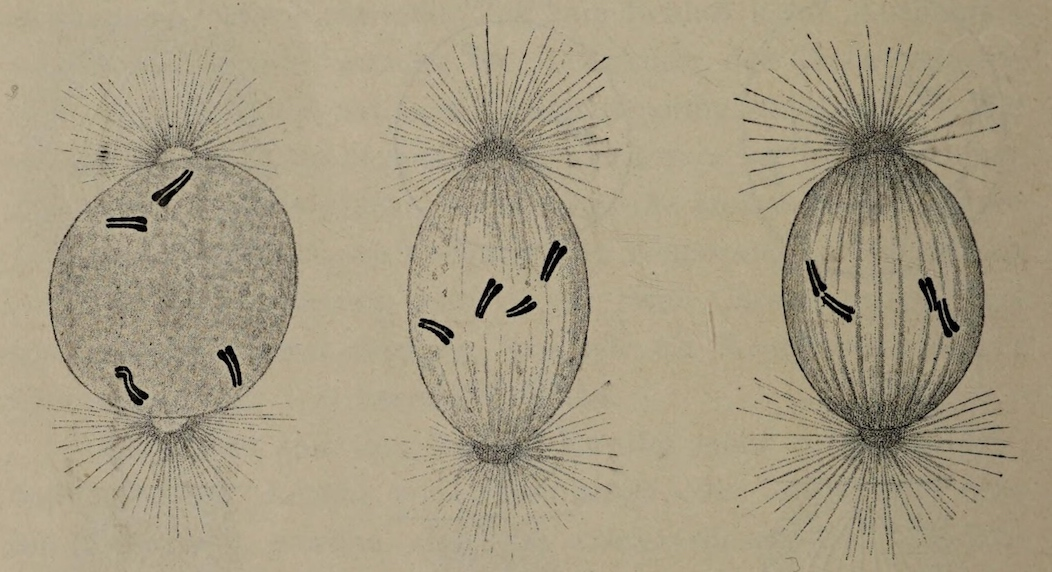
\includegraphics[width=.5\linewidth]{images/intro/boveri-sutton-cropped}
%  \caption[Chromosome segregation during egg maturation in \emph{Ophryotrocha}]{\textbf{Chromosome segregation during egg maturation in \emph{Ophryotrocha}}.}
  % source: https://wellcomecollection.org/works/an45kexq/items?canvas=76
  % Ergebnisse über die Konstitution der chromatischen Substanz des Zellkerns / von Theodor Boveri.. Public Domain Mark
%\end{figure}

\begin{wrapfigure}{r}{.32\textwidth}
  \vspace{-\intextsep}
  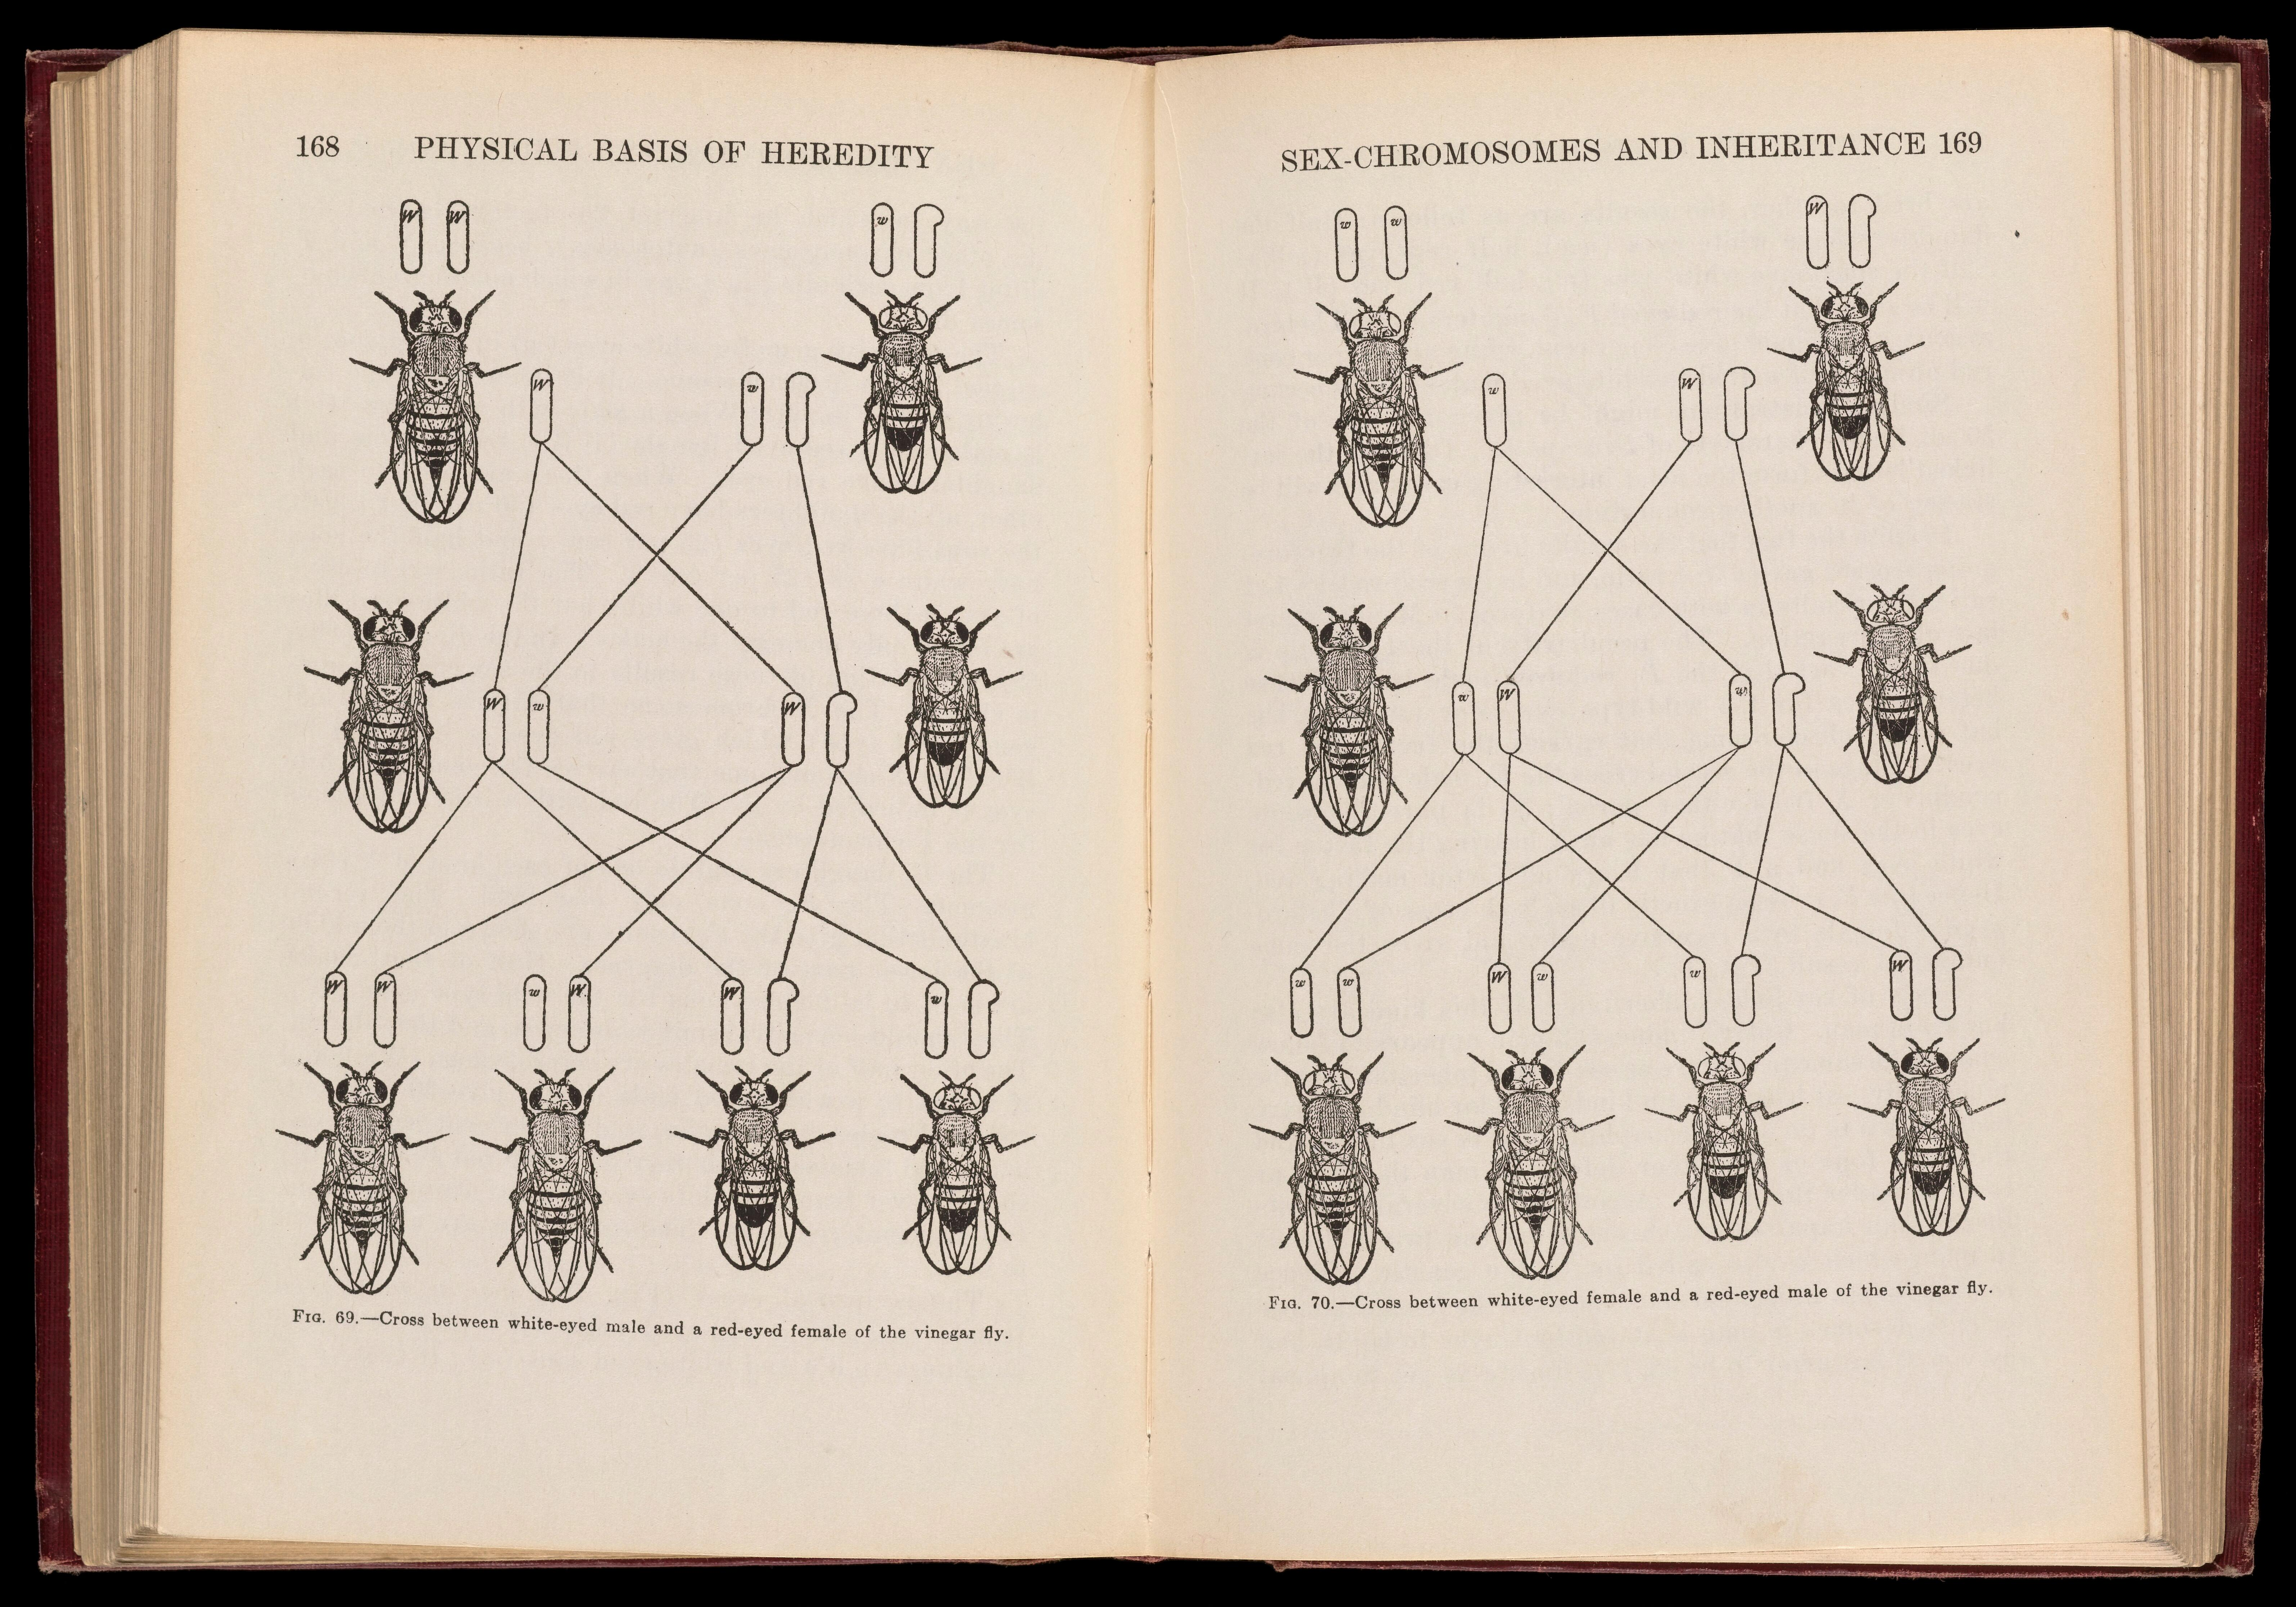
\includegraphics[width=\linewidth]{images/intro/thomas-morgan-fly}
  \caption[Thomas Morgan's fruit fly experiments]{\textbf{Thomas Morgan's fruit fly experiments.} Public domain image from Wellcome Library, London.}

  % source: https://wellcomecollection.org/works/k3rwcqc3/images?id=ey2zux4q
\end{wrapfigure}

The Boveri-Sutton chromosome theory of genetic inheritance followed Mendel's work from 1865 \cite{sutton:1902tx} and was later supported by fruit fly experiments from an initially skeptical Thomas Morgan \cite{morgan:1915tw}. In 1915, Thomas Morgan, Hermann Muller and colleagues published a textbook with their findings describing genetic dominance, sex inheritance and chromosomal crossover. One chapter was interestingly titled \emph{The Chromosomes as Bearers of Hereditary Material} \cite{morgan:1915tw}. In 1927, Hermann Muller discussed that exposure of fruit flies to X-ray radiation induced hundreds of genetic mutations, greatly contributing to the study of genetic mutations and evolution \cite{muller:1927wl}\footnote{Muller's 1927 Science paper \cite{muller:1927wl} that earned him the Nobel prize was not peer-reviewed, cited no references and lacked the methods section \cite{calabrese:2018vl}. This may have happened not only because Muller wanted to be the first to share his hypothesis, but also because he agreed with the criticism by his long-time friend Edgar Alternburg, who believed his data were not strong enough to confirm the induction of mutations \cite{calabrese:2018vl}. It would take until 1930 for Muller to publish results addressing Altenburg's criticism, although Muller was aware of the issues before 1927 \cite{calabrese:2018vl}.}.

% 1928: Frederick Griffith postulates that a "transforming principle" permits properties from one type of bacteria (heat-inactivated virulent Streptococcus pneumoniae) to be transferred to another (live nonvirulent Streptococcus pneumoniae).

At the time, nucleic acids were classified as \emph{thymus nucleic acid} found in animals (specially enriched in the thymus, hence its name) and \emph{yeast nucleic acid} found in plants\footnote{\emph{Yeast nucleic acid} was so named since first extracted from yeasts, considered from the plant kingdom by most scientists at the time. Starting with Ernst Haeckel in 1878, alternative proposed systems clumped fungi together with unicellular organisms instead (kingdoms of Protoctista, Protista, etc.) \cite{haeckel:1878tz}. In 1959, Robert Whitakker suggested a fungi kingdom amid three others \cite{whittaker:1959to}, a proposal that later blossomed into his popular five-kingdom classification system published in 1969 \cite{whittaker:1969to}. In his 1969 article, Whittaker explains why fungi should not be considered plants to his fellow peers.}. However, in 1933, Jean Brachet found evidence of \emph{thymus nucleic acid} in the cell nucleus and of \emph{yeast nucleic acid} in the cytoplasm of eukaryotic cells. His work suggested that both types of nucleic acids were present in the same cell with potentially different roles. During the 1930s, Phoebus Levene identified the phosphate backbone of nucleic acids, including its pentose sugars (deoxyribose and ribose) \cite{levene:1929ug}, which inspired their contemporary nomenclature: \emph{thymus nucleic acid} is now known as deoxyribonucleic acid (DNA) and \emph{yeast nucleic acid} as ribonucleic acid (RNA).
% confirm if in this Levene paper

Although the word \emph{gene} was used since 1909 to abstractly refer to Mendelian factors of inheritance (i.e., the units of heredity) \cite{gayon:2016uj}, Demerec tried to define it in his 1933 publication, \emph{What is a Gene?}, alongside a figure of the \emph{tentative structure of thymus nucleic acids} (DNA):

\begin{displayquote}[\cite{demerec:1933td}]
(...) [A gene] is a minute organic particle, capable of reproduction, located in a chromosome and responsible for the transmission of a hereditary characteristic.
\end{displayquote}

Later in 1941, Edward Tatum and George Beadle hypothesised that each gene is responsible for producing a specific enzyme and demonstrated that radiation-induced mutations could alter the resulting enzyme \cite{beadle:1941vs}. Together with Joshua Lederberg, Tatum demonstrated in 1946 that bacteria can exchange genetic material in a process called genetic recombination \cite{lederberg:1946wl}.

% 1940s, 50s: mobile genetic elements, Barbara McClintock

% 1960s, it was shown in work done in the laboratories of Werner Arber and Matthew Meselson that the restriction is caused by an enzymatic cleavage of the phage DNA, and the enzyme involved was therefore termed a restriction enzyme.
% The 1978 Nobel Prize for Physiology or Medicine was awarded to Werner Arber, Daniel Nathans, and Hamilton O. Smith.[23] The discovery of restriction enzymes allows DNA to be manipulated, leading to the development of recombinant DNA technology that has many applications, for example, allowing the large scale production of proteins such as human insulin used by diabetic patients

\begin{wrapfigure}{R}{.45\textwidth}
%  \vspace{-\intextsep}
  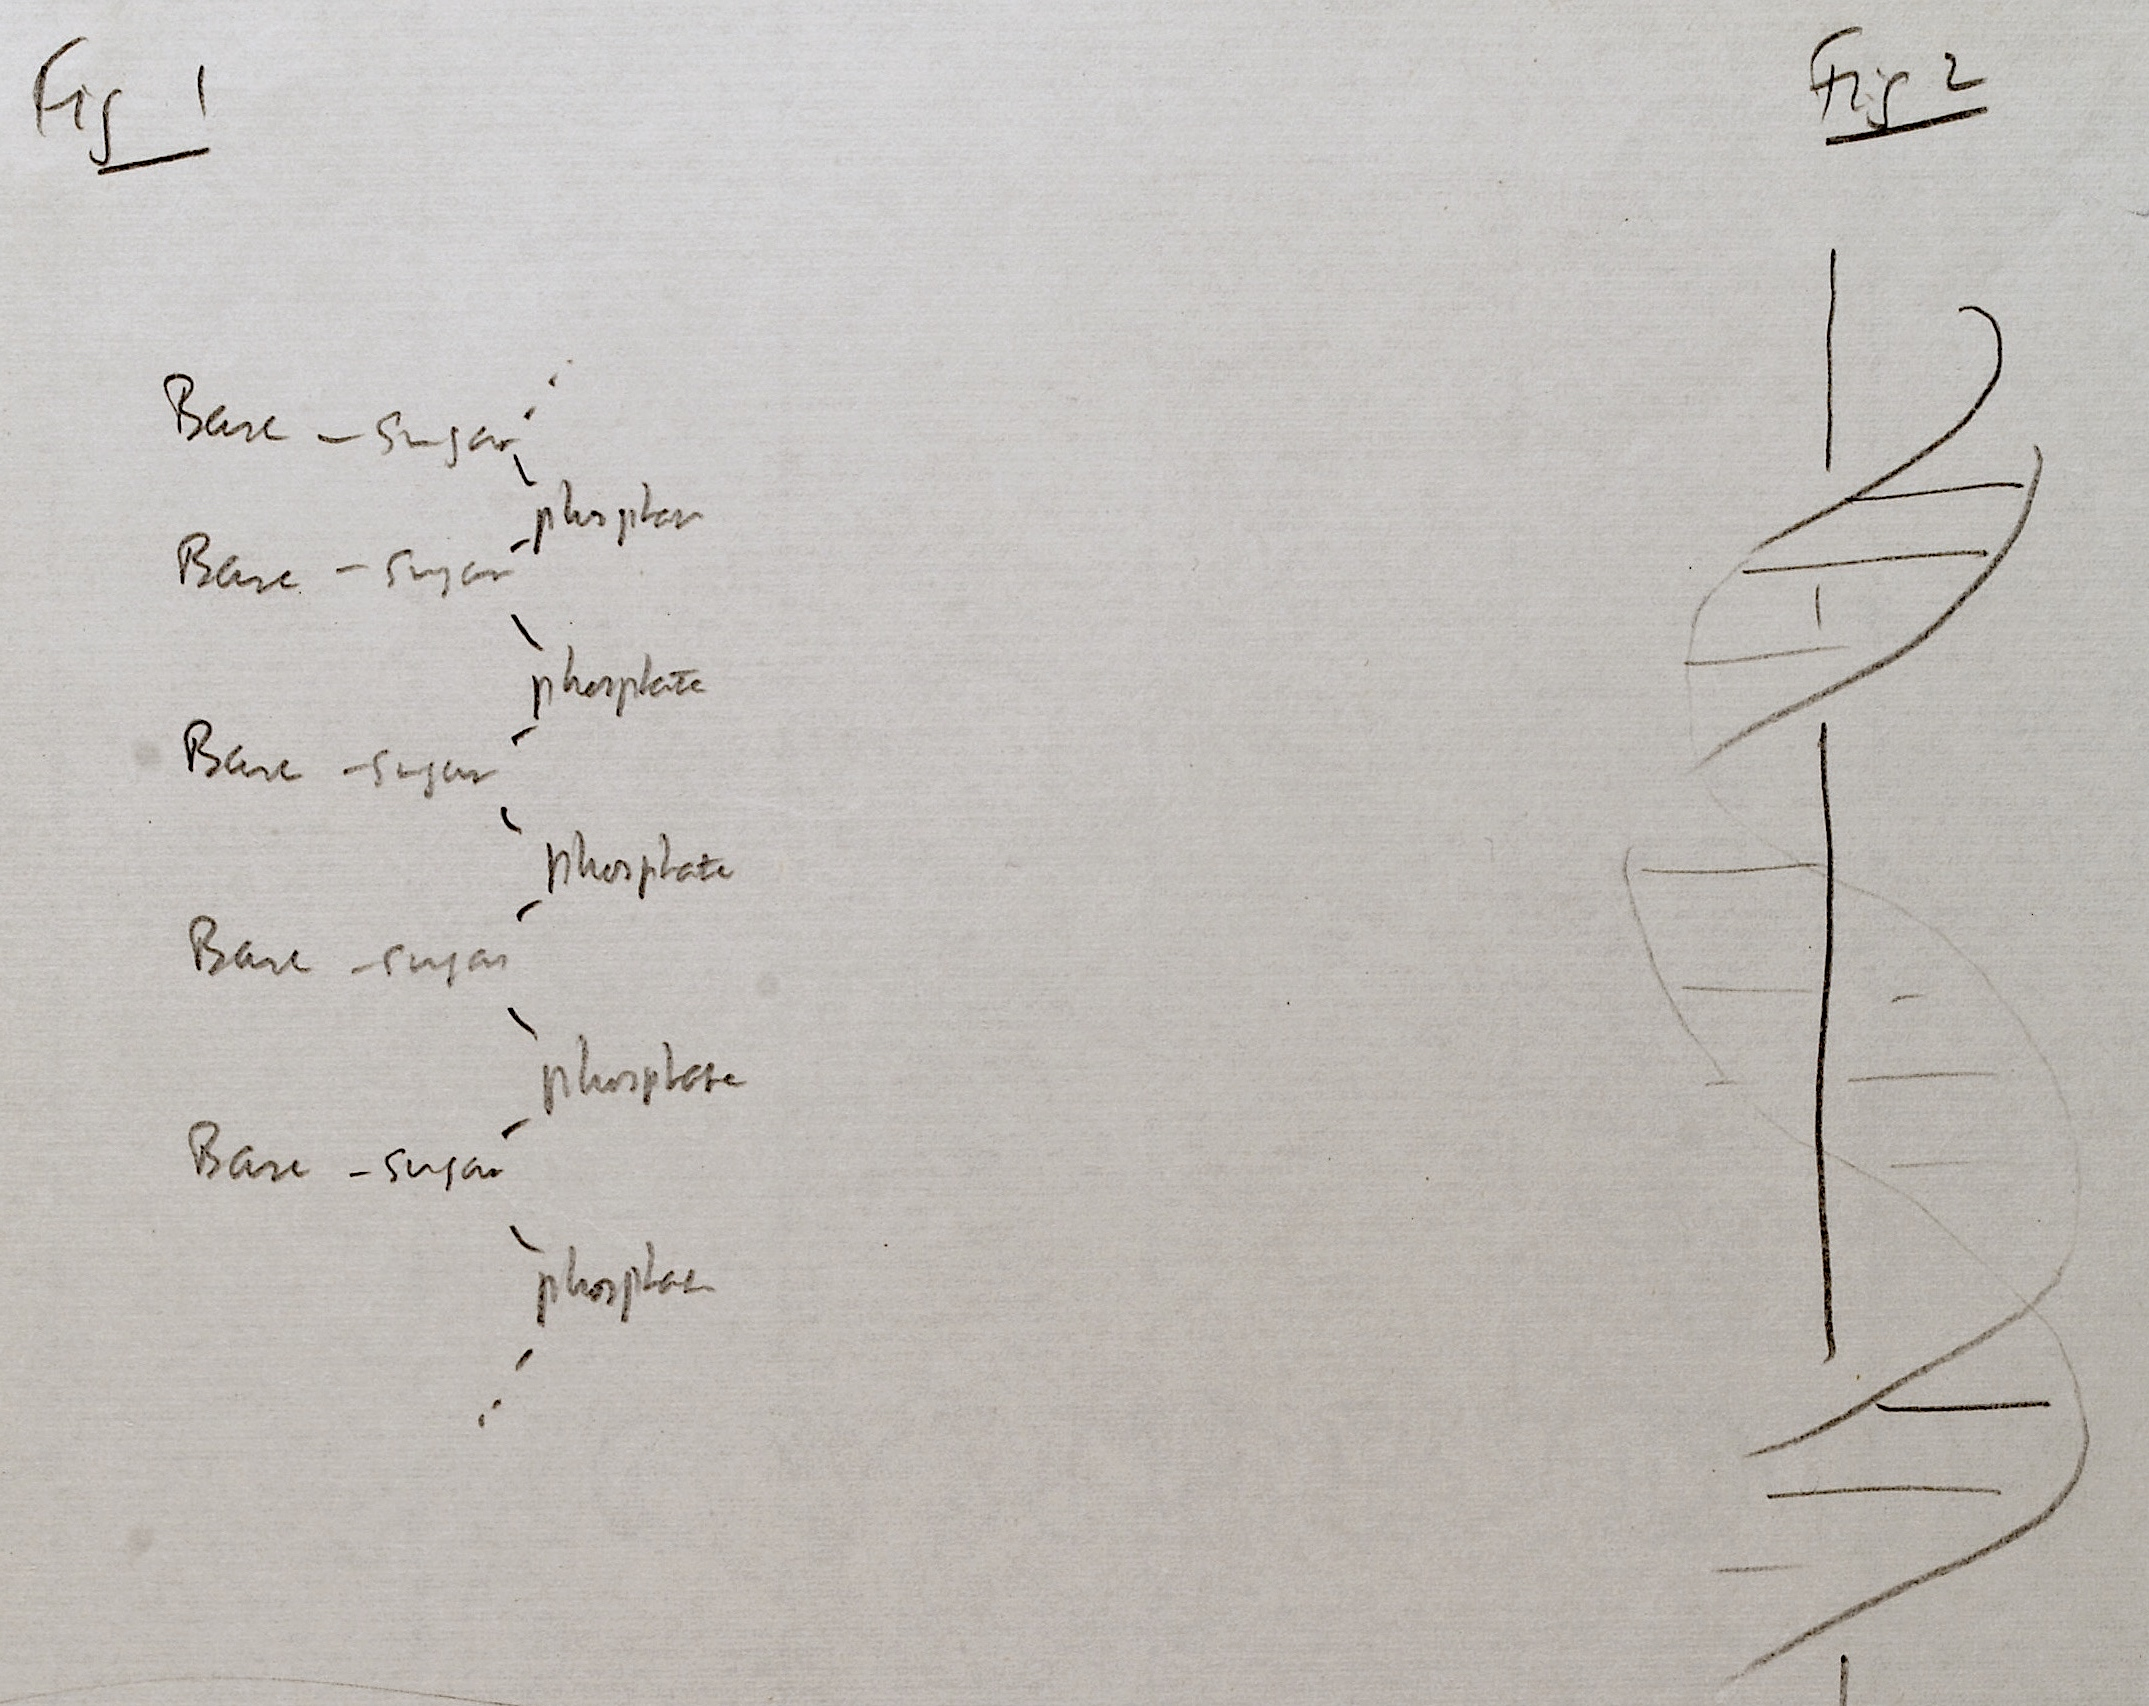
\includegraphics[width=\linewidth]{images/intro/dna_structure_draft_cropped}
  \caption[Figure drafts for a manuscript on DNA structure]{\textbf{Figure drafts for a manuscript on DNA structure} from Francis Crick and James Watson. Public domain image from Wellcome Library, London.}
  \label{fig:dna-structure}
%  \vspace{-\intextsep}
\end{wrapfigure}

In 1952, Alfred Hershey and Martha Chase demonstrated that during viral infection by bacteriophage T2, its DNA, but not any viral protein, enters inside the bacteria \cite{hershey:1952wo}. The viral DNA is enough to produce the DNA molecules found in progeny virus particles. Amid the contemporary belief that proteins were the carriers of hereditary information, the Hershey-Chase experiment complemented previous publications suggesting that that role belonged to DNA \cite{hershey:1952wo}.

The work by Rosalind Franklin and Maurice Wilkins on analysing DNA using X-ray crystallography was crucial to the discovery of DNA's double helix structure, published in 1953 by Francis Crick and James Watson \cite{watson:1953ug}. DNA is composed by two phosphate-sugar chains linked together via hydrogen bonds by pairs of nucleotides: adenine pairs with thymine and cytosine with guanine. Crick and Watson also proposed that this strand complementarity could be important for DNA replication \cite{watson:1953ug}. Afterwards, Arthur Kornberg observed the proposed nucleotide pairing in DNA synthesised by an enzyme that replicates DNA using one of its strands as a template: the DNA polymerase \cite{kornberg:1956wk}.

During a time when not all scientists agreed that nucleic acids played a role in protein synthesis, George Palade described in 1955 the ribosome as \emph{a small particulate component of the cytoplasm} that associates with RNA in the endoplasmic reticulum membrane to perform protein synthesis \cite{palade:1955tf,jacob:1961uh}. The associated RNA was identified as of two types: ribosomal RNA (rRNA) that composed the ribosome itself and \emph{soluble RNA} -- transfer RNA (tRNA) --, found to carry the amino acids for protein synthesis \cite{hoagland:1958vm,jacob:1961uh}. Multiple ribosomes were found to bind to a single RNA molecule (polysomes), allowing for parallelised protein synthesis \cite{warner:1963uj}.

\begin{wrapfigure}{l}{.35\textwidth}
  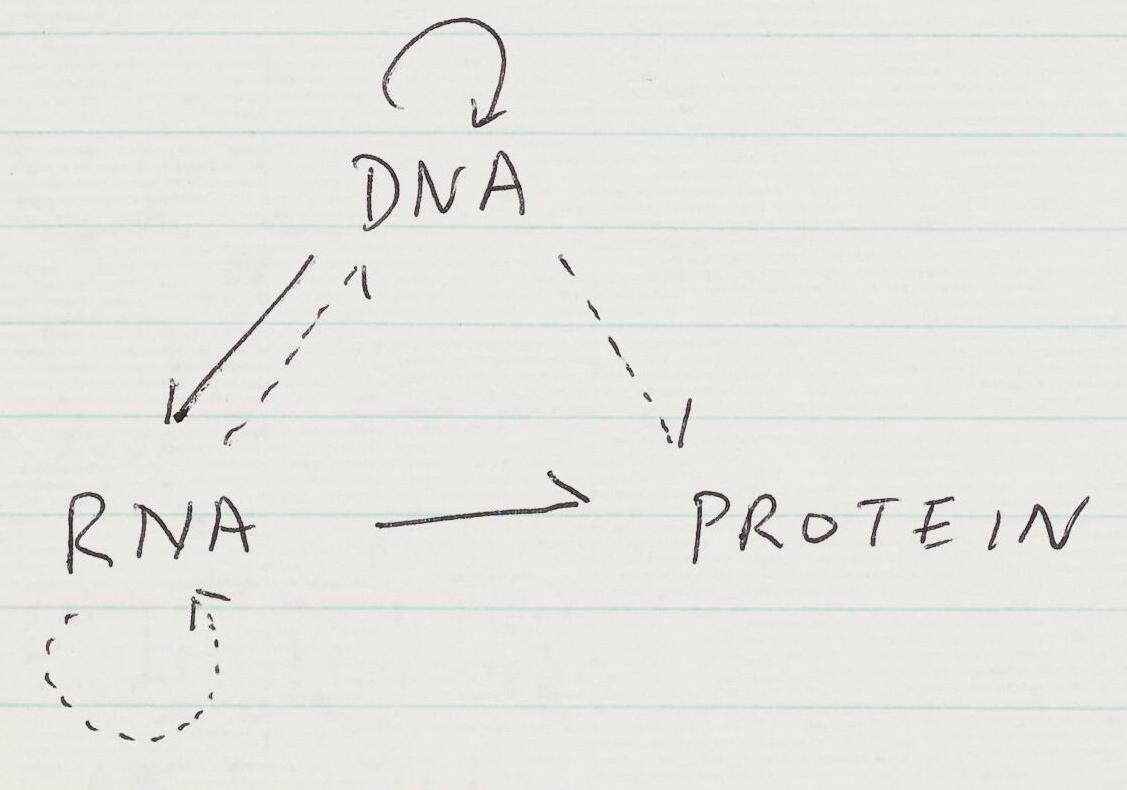
\includegraphics[width=\linewidth]{images/intro/crick-central-dogma cropped}
  \caption[Central dogma of molecular biology]{\textbf{Central dogma of molecular biology} as drafted by Francis Crick. Public domain image from Wellcome Library, London.}
  \label{fig:central-dogma}
  % https://wellcomecollection.org/works/ntzhcpgg/items?canvas=51
\end{wrapfigure}

Piece by piece, the role of DNA and RNA in protein synthesis was becoming clearer. Francis Crick proposed in 1958 that the genetic information flows from DNA to protein via RNA: the \emph{central dogma of molecular biology} \cite{crick:1958ws,crick:1970aa}. It was also hypothesised at that time that triplets (\emph{codons}) of the four nucleotides found in nucleic acids were necessary to produce each of the 20 universally-found types of amino acids that compose a protein \cite{crick:1958ws,crick:1961ui} and that those amino acids would be responsible for the protein's three-dimensional structure -- and consequently, its functionality \cite{crick:1958ws}. It took less than a decade to unravel which codons code for which aminoacid, an important breakthrough that allowed to predict protein sequences from DNA and RNA via the so-called universal genetic code \cite{khorana:1966vr,crick:1968wg}. % universal to virtually all species
In 1959 and 1960, DNA-dependent RNA polymerase, an enzyme that synthesises RNA from DNA and common to all living organisms, was independently described by the labs of Samuel Weiss, Jerard Hurwitz and Audrey Stevens \cite{hurwitz:1960uf,weiss:1959vp,stevens:1960ue} \footnote{In 1955, Severo Ochoa and Marianne Grunberg-Manago discovered the polynucleotide phosphorylase (PNPase) enzyme that they thought to synthesise RNA polymers from DNA \cite{grunberg-manago:1956wb}. Ochoa was erroneously awarded a Nobel prize in 1959 for discovering the biological mechanism of RNA synthesis.}.

% RNA structure?
% Doty, P., Boedtker, H., Fresco, J.R., Haselkorn, R. and Litt, H. (1959) PNAS 45, 482-498. 10
% Fresco, J.R., Alberts, B.M. and Doty, P. (1960) Nature 188, 98-101.

François Jacob and Jacques Monod speculated in 1961 that ribosomal protein synthesis required an intermediate molecule with the template message to convert from DNA to protein and that would act as the \emph{messenger} \cite{jacob:1961uh,brenner:1961ve}. Unlike many of their contemporaries, they dismissed the known rRNA (and tRNA) molecules as the template for protein synthesis, given that they did not reflect the base composition of DNA, among other properties \cite{jacob:1961uh}. Based on contemporary experiments, Jacob and Monod proposed unstable RNA molecules as relevant candidates and named them messenger RNA (mRNA) \cite{jacob:1961uh,brenner:1961ve}. Making the distinction between \emph{structural genes} and \emph{other, functionally specialized, genetic determinants}, Jacob and Monod also discussed the induced activation of repressors in mRNA synthesis \cite{jacob:1961uh}.

In the 1969 publication entitled \emph{Gene Regulation for Higher Cells: A Theory}, Roy Britten and Eric Davidson proposed that:

\begin{displayquote}[\cite{britten:1969va}]
Cell differentiation is based almost certainly on the regulation of gene activity, so that for each state of differentiation a certain set of genes is active in transcription and other genes are inactive.
\end{displayquote}

Among the first ideas of its kind, Britten and Davidson theorised about the intricate networks of gene regulation as fine-tuned systems in higher organisms based on the redundancy of different genomic elements and feedback loops. As they wrote, large genome sizes do not imply an increase in the number of genes compared to smaller genomes, but rather an increase in regulation complexity: \emph{a large amount of DNA [including repeated DNA sequences] could be devoted to regulatory function}, for instance by sequence-specific binding of RNA from another gene \cite{britten:1969va}. 

In the beginning of the 1970s, the first studies on RNA processing were published. At the time, two types of RNA were distinguished inside the nucleus: ribosomal precursor RNA molecules that yield cytoplasmic rRNA and heterogeneous nuclear RNA (hnRNA) whose composition \emph{resembles that of DNA} \cite{darnell:1971tg}. \emph{Polyadenylic acid} (polyA) sequences ranging from 150 to 250 nucleotides were found to be added to the 3$'$ end of hnRNAs and cytoplasmic mRNAs, the first sign of eukaryotic RNA processing \cite{darnell:1971tg,edmonds:1971vr}. James Darnell and colleagues thus proposed that hnRNAs and cytoplasmic mRNAs were related: the polyA sequence is added to hnRNAs post-transcriptionally in order to enable the export of nuclear RNAs to the cytoplasm, which are later found to be associated with ribosomes for protein synthesis \cite{darnell:1971tg,edmonds:1971vr}. Later in 1974, the addition of a 5$'$-methylated cap was found in hnRNA and cytoplasmic mRNA and was proposed as an eukaryotic post-transcriptional RNA modification that protects the 5$'$-end of RNAs from degradation enzymes \cite{perry:1974uj,rottman:1974tk}.
% Other functions of polyA tails and 5' cap?

% Most RNAs are non-coding: 97\% in eukaryotes?

% protein synthesis occurs in the cytoplasm
% RNA degradation?

% From the mid 1970s, through studies of bacteria, Tomas Lindahl showed how certain protein molecules, repair enzymes, remove and replace damaged parts of DNA. These discoveries have increased our understanding of how the living cell works, the causes of cancer and aging processes.

\subsection{Alternative splicing}

% A gene is a segment of DNA that is transcribed to RNA and, in case of mRNA, may later be encoded as a protein. The whole process from gene to its product is known as gene expression and summarises multiple, complex steps that occur within the cell to maintain its well-being. Such processes include RNA synthesis (transcription), RNA splicing and protein synthesis (translation).

% It was also Crick that suggested we would study evolution by comparing sequences across species.

First reported in mammalian cells infected with human adenovirus 2 \cite{berget:1977wp,chow:1977wn} and later observed in endogenous mammalian and eukaryotic genes \cite{brack:1977we,early:1980wq}, mRNA-DNA hybridisation experiments starting in 1977 suggested that genes are composed by intervening non-coding sequences, based on experiments from Richard Roberts, Philip Sharp and colleagues. During or after transcription of the precursor mRNA (pre-mRNA), a process called \emph{splicing} is responsible for excising segments of the pre-mRNA (named introns), leaving behind the sequences required for protein synthesis (exons) \cite{berget:1977wp,chow:1977wn,gilbert:1978wr}. Moreover, multiple different transcripts may be produced from the same primary transcript by \emph{alternative splicing} of segments of their sequence, thus promoting transcriptome diversity \cite{berget:1977wp,chow:1977wn,chow:1978wk,nevins:1978tt,schmucker:2000wf}.

\begin{figure}[!b]
  \vspace{-\intextsep}
  \centering
  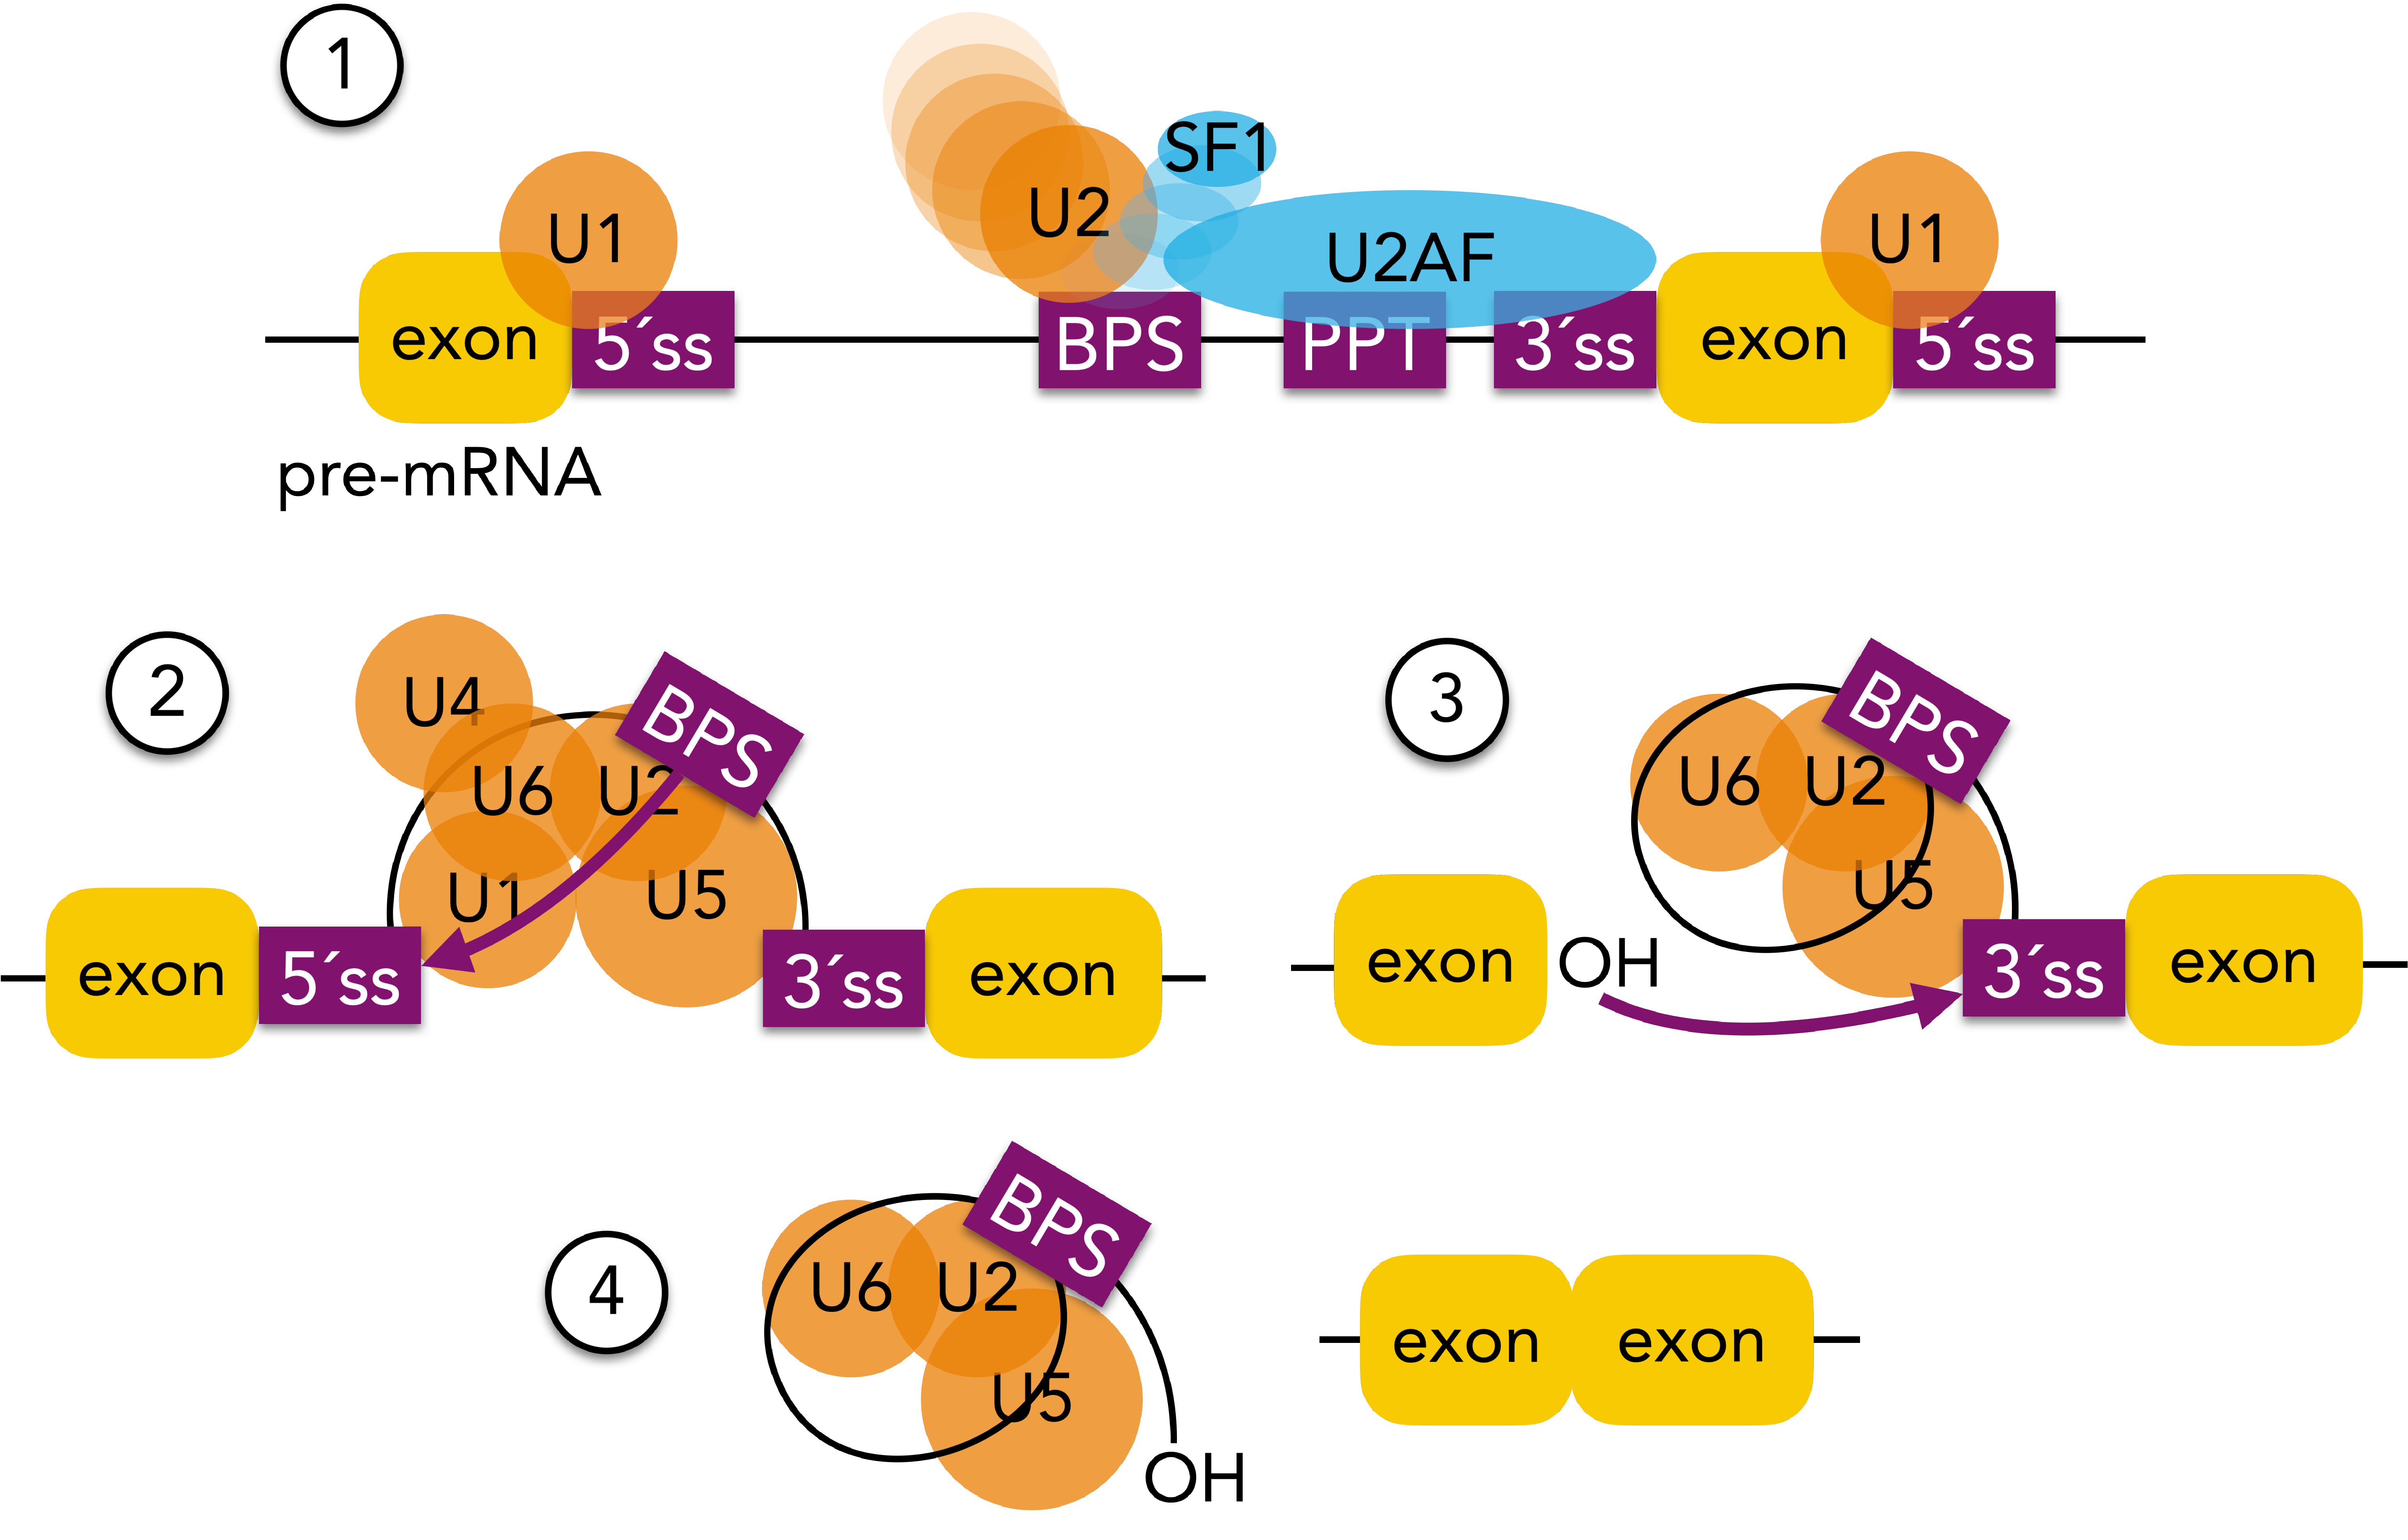
\includegraphics[width=.6\linewidth]{images/intro/spliceosome-assembly}
  \vspace{-.8\intextsep}
  \caption[Spliceosome assembly and splicing reactions]{\textbf{Spliceosome assembly and splicing reactions.} (1) U1 snRNP binds to the 5$'$ splice site (5$'$ss), whereas the splicing factor 1 (SF1) and U2AF proteins bind to the branch point site (BPS), the polypyrimidine tract (PPT), and 3$'$ splice site (3$'$ss). The interaction between U1 and U2 snRNPs results in the formation of the pre-spliceosome. (2) The first splicing reaction is performed after the recruitment of the U4/5/6 snRNPs through a nucleophilic attack from the adenosine in the BPS to the 5$'$ss of the upstream exon. (3) The intron lariat is then formed. The free 3$'$ hydroxyl group performs a nucleophilic attack to the phosphate of the 3$'$ splice site of the downstream exon. (4) Finally, the intron lariat is released and both exons are ligated. Image created by me for \cite{gallego-paez:2017wc} (adapted).}
  \label{fig:spliceosome-assembly}
\end{figure}

In 1985, an RNA-protein complex composed by the so-called U1, U2, U4, U5 and U6 small nuclear ribonucleoproteins (snRNPs) was reported to be central for RNA splicing: the spliceosome \cite{grabowski:1985vm}. The spliceosome recognises splice sites (conserved sequences located at the 5$'$ and 3$'$ ends of an intron) and the branch point sequence and polypyrimidine tract (located just upstream of the intron's 3$'$ end) \cite{mount:1982tu,black:1985ul}. The spliceosome then catalyses the excision of introns from pre-mRNA in two transesterification steps: (1) the 5$'$ end of the intron is cleaved and united to the conserved adenosine in the branch point sequence, forming an intermediary intron lariat, and then (2) the 3$'$ end of the intron is cleaved, releasing the intron lariat, and the two flanking exons are ligated (\autoref{fig:spliceosome-assembly}) \cite{grabowski:1985vm,ruskin:1985vl,horowitz:1993wq}. The intron lariat is debranched (i.e., converted to a linear form) before its degradation \cite{ruskin:1985vl,arenas:1987vc}.

However, not all introns require the presence of the spliceosome to be spliced out. During the 1980s, Thomas Cech identified rRNAs that underwent self-splicing by breaking and forming covalent bonds with no associated proteins \cite{kruger:1982wk}, whereas Sidney Altman identified that the RNA subunit of a complex of proteins and RNAs (ribonulceoprotein complex) was essential for tRNA splicing and was able to cleave tRNAs \emph{in the total absence of proteins} \cite{altman:1986wp}. These RNAs with enzyme-like proteins were named ribozymes and they may have been a paramount mechanism that conferred evolutionary flexibility in life forms of yore, one of the pillars that originated the RNA world hypothesis \cite{kruger:1982wk,gilbert:1986td}. From fungi to plants and vertebrates, many spliced genes across eukaryotic organisms share consensus sequences at their branch point, as well as their 5$'$ and 3$'$ splice sites, potentially making splicing one of the first molecular catalysts that appeared in living beings \cite{sharp:1985th}. Interestingly, primary transcripts from yeast can be spliced with the mammalian splicing machinery \cite{sharp:1985th}.
% conservation of AS across tissues and organisms (Barbosa-Morais et al.)

By 1989, it was known that alternative splicing is differentially regulated across cell types, development stages and tissues in eukaryotes, i.e., the same gene can lead to different, context-dependent spliced transcripts \cite{smith:1989tr}. This regulation occurs via the interplay between trans-acting factors -- RNA-binding proteins (RBPs) -- and the cis-acting sequence elements to which they bind to, promoting or repressing the inclusion of alternative sequences \cite{smith:1989tr}. Multiple types of alternative splicing have also been described, including skipped exons, mutually exclusive exons, alternative 5$'$ and 3$'$ splice sites, alternative first and last exons and intron retention \cite{smith:1989tr}.
% add figure + cite newer review on splicing

% 1989-1996: minor spliceosome splices less than 1\% of all human introns

% By the early1990s, the spliceosome was shown to be assembled at each splice event and to act in a dynamic stepwise process that links exons in mRNAs (for review, see Wahl et al. 2009).

Among other molecular mechanisms, alternative splicing made clear that an organism complexity is not limited to the genome size or the number of protein-coding genes \cite{lee:2015tt}. After all, the Australian lungfish (\emph{Neoceratodus forsteri}) is the animal with the largest haploid genome size (44 000 million base pairs), 14 times larger than that of humans (3 000 million base pairs) and 244 times larger than the fruit fly \emph{Drosophila melanogaster} (180 million base pairs) \cite{meyer:2021vn,adams:2000tj,myers:2000wk}. And yet, their genomes harbour 31 000, 20 000 and 14 000 protein-coding genes, respectively, numbers in the same order of magnitude, whereas the remaining genomes of these species are composed of intergenic regions and introns with high repeat content \cite{meyer:2021vn,adams:2000tj,myers:2000wk}. Notably, 38 000 alternative transcripts may be generated from a single gene in the fruit fly (\emph{Dscam}): some of those transcripts are suggested to play a role in the immune system and may lead to more antigen diversity, thus increasing the evolutionary flexibility of the fruit fly  \cite{schmucker:2000wf}.
% how many functional proteins? what more about this example? maybe useful to talk about other topic such as trans/cis-acting elements or spliceosome?

% 90-95\% of human genes are spliced
% variation of AS across tissues

% Coupling of Transcription and Splicing?

Alternative splicing is deregulated in multiple disease contexts, including cancer, neurodegeneration and muscular dystrophies \cite{gallego-paez:2017wc,montes:2019ww}. For instance, changes in splicing factors and subsequent  perturbations to splicing can affect multiple hallmarks of cancer \cite{zhang:2021wn}. Therefore, multiple potential splicing-targeting therapies have been developed based on antisense oligonucleotides, small molecules and novel techniques \cite{montes:2019ww}.
% Discuss disease-related NMD?
% Alternative splicing in ncRNAs?

% AS during organ development: https://www.nature.com/articles/s41588-021-00851-w

% Around 1980, Michael Smith developed a method by which combined DNA building blocks could be artificially bonded with DNA molecules that were then inserted into an organism where they were copied. The result was an artificial mutation; the genome was altered so that specific amino acids in the proteins were replaced. The opportunities this method provides to tailor proteins have been of major importance in both research and industry.
% In 1989, through studies of bacterial viruses, Paul Modrich showed how methyl groups attached to the DNA molecule act as signals for repairing incorrect replications of DNA. These discoveries have increased our understanding of how the living cell works, the causes of cancer and about aging processes.
% 1998: RNAi -- gene silencing discovered by Andrew Fire and Craig Mello

\section{Bioinformatics}

% The fact that we need to specifically name the computer-aided analysis as sub-field of biological research demonstrates how bioinformatics is not as widely used as it should.

% 1. sequencing, annotation and comparison
% 2. comparative sequence analysis
% 3. expression analysis
% 4. structure prediction
% 5. network modelling

Bioinformatics is a multidisciplinary field based on the usage and development of computer programs to analyse large-scale biological data \cite{gauthier:2018ws}. The first bioinformatic analyses were performed on proteins. Following Sanger's work in 1959 on identifying the amino-acid composition of protein insulin in multiple species, many proteins started being sequenced \cite{sanger:1955uw,ryle:1955wf,harris:1956ut,gauthier:2018ws}.
% He used acids to break the molecule into smaller parts, which were separated from one another with the help of electrophoresis and chromatography. Further analyses determined the amino acid sequences in the molecule's two chains, and in 1955 Frederick Sanger identified how the chains are linked together.
Pointing to such studies, Crick predicted in 1958:

\begin{displayquote}[\cite{crick:1958ws}]
Biologists should realize that before long we shall have a subject which might be called 'protein taxonomy' - the study of the amino acid sequences of the proteins of an organism and the comparison of them between species.
\end{displayquote}

For that to come to fruition, there was a need to sequence many more proteins from different species. A technique known as Edman degradation was popularly used at the time to sequence proteins: the amino acids were identified by chemically fragmenting the protein, identifying the first 50-60 amino acids of each fragment. Afterwards, the full protein sequence is reconstructed based on its overlapping fragments, a long and tedious process performed by hand \cite{gauthier:2018ws,edman:1949ww}. All these limitations meant that only 6 different proteins were fully sequenced by 1962 \cite{dayhoff:1962up}. To overcome those difficulties in the reconstruction step, Margaret Dayhoff and Robert Ledley developed COMPROTEIN, the first bioinformatics program \cite{gauthier:2018ws,dayhoff:1962up}. COMPROTEIN allows to compare a high number of small peptide fragments and suggests possible full protein sequences \cite{dayhoff:1962up}. By 1965, the number of published protein sequences grew up to 65 and were published by Dayhoff in the first protein database, otherwise known as the book entitled \emph{Atlas of Protein Sequence and Structure}\cite{dayhoff:1965vv}.

In 1963, Linus Pauling and Emile Zuckerkandl discussed that cross-species comparative analysis of protein sequences could help determine the original protein sequence of their common ancestor and measure the evolutionary distance of the sequence of each species to that of their common ancestor \cite{pauling:1963uo}. However, these protein comparison methods were performed by hand, which meant that they were only practical for closely-related proteins such as homologs from different mammals \cite{gauthier:2018ws}. Since 1970, computer-assisted phylogenetics started being a reality with the introduction of the Needleman-Wunsch algorithm \cite{needleman:1970vq} and variants, such as the Smith-Waterman algorithm \cite{smith:1981up}. These programs computationally measure the distance between two sequences by pair-wise comparison of amino acids between protein sequences \cite{needleman:1970vq,smith:1981up}.

% Substitution matrices in 1978:
% - Dayhoff, M.O., Schwartz, R.M., Orcutt, B.C. (1978) "A model of evolutionary change in proteins." In "Atlas of Protein Sequence and Structure, vol. 5, suppl. 3," M.O. Dayhoff (ed.), pp. 345-352, Natl. Biomed. Res. Found., Washington, DC.
% - Schwartz, R.M., Dayhoff, M.O. (1978) "Matrices for detecting distant relationships." In "Atlas of Protein Sequence and Structure, vol. 5, suppl. 3," M.O. Dayhoff (ed.), pp. 353-358, Natl. Biomed. Res. Found., Washington, DC.

% conservation, structural conformation, functional domains

% when did computers started being used?

Years after automatic protein sequencing machines being available based on Edman degradation -- \emph{protein sequenators} as first called in 1967 \cite{edman:1967tc} --, DNA sequencing methods were presented based on electrophoresis: the enzymatic Sanger method (also known as dideoxy method) \cite{sanger:1977vp} and the chemical degradation method Maxam-Gilbert sequencing \cite{maxam:1977vy}. These tedious and slow processes required manual intervention \emph{at both the experimental and interpretative levels} \cite{hood:1987va}.

\begin{wrapfigure}{r}{.4\textwidth}
  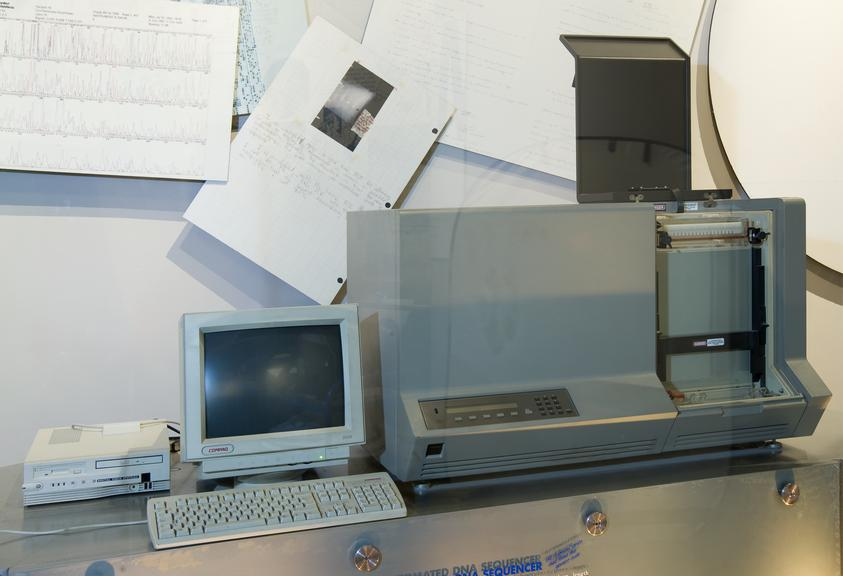
\includegraphics[width=\linewidth]{images/intro/dna-sequencer}
  \caption[Applied Biosystems DNA sequencer prototype]{\textbf{Applied Biosystems DNA sequencer prototype.} Public domain image from Science Museum Group Collection, London.}
  \label{fig:dna-sequencer}
\end{wrapfigure}

Leroy Hood and Lloyd Smith published in 1987 a report on an instrument to automate the experi\-mental procedure based on the Sanger method followed by computer analysis to determine the sequence of DNA fragments (i.e., base calling): the Applied Biosystems DNA sequencer, the first commercialised automated machine to sequence DNA (\autoref{fig:dna-sequencer}) \cite{hood:1987va}. Their article also discusses experimental issues with sequencing repetitive DNA regions, storing and sharing the big amount of data produced in the following years in \emph{data banks}, as well as the algorithms required to quickly retrieve sequence from those databases -- obstacles that impaired large-scale DNA sequencing, specially of the whole human genome \cite{hood:1987va}.

Later, the advent of Next-Generation Sequencers (NGS) allowed the massive parallel sequencing of nucleic acids. These techniques use alternative methods to Sanger sequencing to efficiently sequence DNA or RNA fragments simultaneously.

As the techniques to retrieve biological data were optimised, more and more data started being generated and published in public databases such as the Protein Data Bank \cite{protein-data-bank:1971tm} and GenBank \cite{burks:1985ts}. Computers were no longer optional to survive the tsunami of biological data and new popular bioinformatic algorithms started to emerge.
\begin{wrapfigure}{r}{.4\textwidth}
  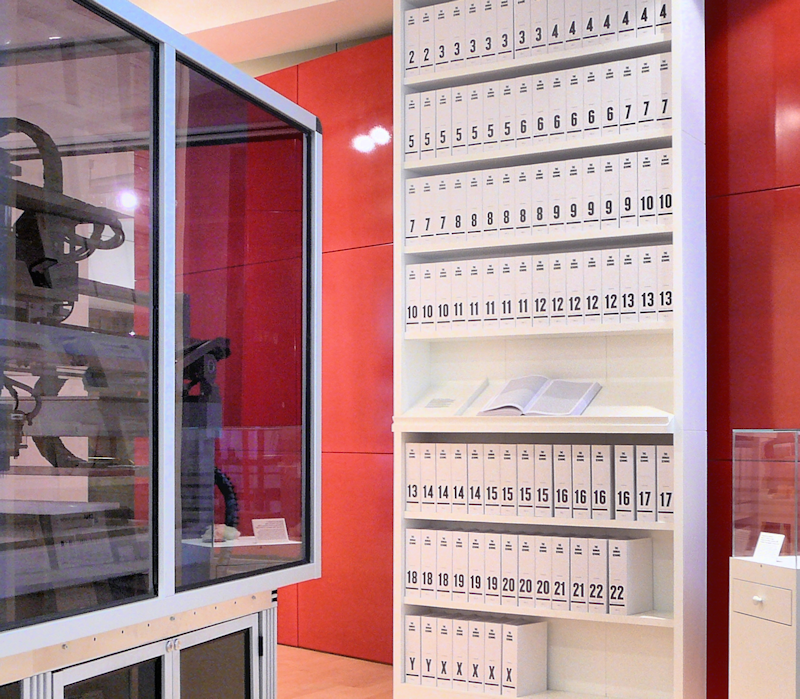
\includegraphics[width=\linewidth]{images/intro/human-genome-project-bookcase}
  \caption[Human genome project bookcase]{\textbf{Human genome project bookcase.} More than a hundred volumes contain the printed human genome sequence located in the Wellcome Collection, London. Public domain image from Wikipedia.}
  \label{fig:dna-sequencer}
\end{wrapfigure}
More advanced sequence aligners, such as CLUSTAL in 1988, efficiently allowed to align multiple sequences of amino acids or nucleotides from pairwise sequences \cite{higgins:1988ul}. In 1990, BLAST was presented as an efficient algorithm to quickly compare a DNA or protein sequence against the ever-increasing number of molecular sequences from biological databases \cite{altschul:1990vt}.

In 1995, the first complete sequence of a free-living organism was published for bacterium \emph{H. influenzae} \cite{fleischmann:1995vz}. From 1996 to 2000, the whole genomes of multiple organisms were sequenced, including for yeast \emph{S. cerevisiae} \cite{goffeau:1996tk}, nematode \emph{C. elegans} \cite{the-c.-elegans-sequencing-consortium:1998wf}, fruit fly \emph{D. melanogaster} \cite{myers:2000wk,adams:2000tj}, and plant \emph{A. thaliana} \cite{the-arabidopsis-genome-initiative:2000tm}. In 2004, the Human Genome project was considered finished with its goal of publishing the human haploid genome sequence to the scientific community, leaving 8\% to be determined due to technical limitations \cite{consortium:2004wi,nurk:2021up}. Many advantages flow from sequencing whole genomes, specially the \emph{near complete} human genome:

\begin{displayquote}[\cite{consortium:2004wi}]
It allows systematic searches for the causes of disease -- for example, to find all key heritable factors predisposing to diabetes or somatic mutations underlying breast cancer -- with confidence that little can escape detection. It facilitates experimental tools to recognize cellular components -- for example, detectors for mRNAs based on specific oligonucleotide probes or mass-spectrometric identification of proteins based on specific peptide sequences -- with confidence that these features provide a unique signature. It allows sophisticated computational analyses -- for example, to study genome structure and evolution -- with confidence that subtle results will not be swamped or swayed by noisy data. At a practical level, it eliminates tedious confirmatory work by researchers, who can now rely on highly accurate information. At a conceptual level, the near-complete picture makes it reasonable for the first time to contemplate systems approaches to cellular circuitry, without fear that major components are missing.
\end{displayquote}

% Third-generation sequencing: longer reads
More recently, the Telomere-to-Telomere (T2T) consortium exploited current long-read sequencing (third-generation sequencing), along with other sequencing technologies, in order to fully unravel the gapless assembly of the human genome sequence for use in biomedical research \cite{nurk:2021up} \footnote{Although the most recent T2T pre-print manuscript from 2021 describes ongoing work for the missing chromosome Y \cite{nurk:2021up}, the latest assembly published in 24 January 2022 (CHM13 T2T v2.0) includes the full human genome sequencing: \alink{ncbi.nlm.nih.gov/assembly/GCA_009914755.4}.}.

\subsection{Transcriptomics}

The term \emph{omics} encompasses all fields in life sciences that analyse large-scale data to better understand the molecular world \cite{yadav:2007uy}. The first word using the \emph{-omics} suffix dates back to a 1986 conference meeting among peers and beers. While discussing the name for a new journal intended to include sequencing data, gene mapping and new genetic technologies, Thomas Roderick proposed a name to illustrate a \emph{new way of thinking about biology}: genomics \cite{yadav:2007uy,kuska:1998ta}. The genomics field is concerned with the study and cross-species comparison of genomes \cite{kuska:1998ta}.

In the same vein, transcriptomics is the field that studies the transcriptome: the full set of RNA transcripts\footnote{Depending on the context, the term \emph{transcriptome} may exclusively refer to the study of mRNA transcripts instead of all RNA transcripts.}, as first defined in 1996 \cite{pietu:1999tl}. Transcriptomics usually leverages data generated from high-throughput technologies that allow to simultaneously analyse the expression of multiple RNAs. Diverse technologies have been proposed for the large-scale study of transcripts since the 1990s, including:

\begin{itemize}
	\item \textbf{Expressed Sequence Tags (EST)}: proposed in 1991 as a pilot experiment to focus on the genes identified as expressed via the Human Genome project \cite{adams:1991ua}. EST allow to identify random sequences of complementary DNA (cDNA), i.e., reverse transcribed mRNA sequences.%\footnote{The article starts with an interesting motivation: \emph{The Human Genome is estimated to consist of 50 000 to 100 000 genes, up to 30 000 of which may be expressed in the brain.} \cite{adams:1991ua}. The number of genes is still debated nowadays, but a recent pre-print estimates them to be around 43 162 genes, of which 21 306 are protein-coding genes \cite{pertea:2018ty}.}
	\item \textbf{Serial Analysis of Gene Expression (SAGE)}: developed in 1995 for the \emph{quantitative and simultaneous analysis of a large number of transcripts} \cite{velculescu:1995vx}.
	\item \textbf{Microarrays}: first mentioned in a 1995 study as a method to simultaneously measure the expression of multiple genes in an high-density array with small wells via cDNA hybridisation \cite{schena:1995tu}. According to the article: \emph{The large and expanding database of complementary DNA (cDNA) sequences from many organisms presents the opportunity of defining these patterns at the level of the whole genome} \cite{schena:1995tu}. The first genome-wide microarray study was later conducted in yeast during 1997 \cite{lashkari:1997wh}, followed by the whole human transcriptome based on a cDNA library from infant human brain in 1999 \cite{pietu:1999tl}.
	\item \textbf{Short-read RNA sequencing (RNA-seq)}: first mentioned in 2008 as a novel quantitative technique based on the Illumina platform to sequence cDNA fragments in a massively parallel method \cite{nagalakshmi:2008vs}. This method is followed by computational mapping of resulting short reads (spanning 50 bases at the time, currently along the lines of 150-200 bases) to a genome of reference, allowing to unravel the transcriptional regions of the yeast. More accurate and sensitive than microarray methods, RNA-seq can quantify more lowly-expressed transcripts than microarrays by avoiding cross-hybridisation issues. RNA-seq data also allows to accurately identify exon boundaries and therefore introns, crucial for alternative splicing analysis \cite{nagalakshmi:2008vs}.
	\item \textbf{Long-read RNA-seq}: RNA-seq methods that generate reads between 1 000 and 10 000 bases, allowing to sequence full transcripts -- specially advantageous to sequence overly similar transcripts \cite{conesa:2016vw}. Given the higher error-rate and cost of this technology compared to short-read RNA-seq, combining both short- and long-read technologies allows to mitigate the technical limitations of both approaches \cite{conesa:2016vw}.
%	\item \textbf{Direct RNA-seq}: direct sequencing of RNA molecules without modification or reverse transcription \cite{ozsolak:2009ub}. This technology aims to reduce technical biases in RNA sequencing by avoiding problems with the generation of artefactual cDNAs and low yield of cDNA from the inefficient reverse transcriptases \cite{ozsolak:2009ub}.
%	\item \textbf{Single-cell RNA-seq (scRNA-seq)}: reported in 2009, 
%	\item \textbf{Ribosome profiling}:
%	\item \textbf{Spatial RNA-seq}:
%	\item \textbf{Nascent RNA sequencing}: 
\end{itemize}

% paired-end vs single-end?
\subsubsection{RNA-seq data analysis}

Before transcriptomic analyses, transcripts are isolated by first disrupting cell membranes and neutralising RNA-degrading enzymes (RNases). As over 90\% of the extracted RNA is ribosomal, depletion of rRNAs and/or enrichment of the desired species are required for proper analysis. Most datasets currently enrich for polyadenylated RNAs (i.e., isolating mostly mature mRNAs).

% https://pubmed.ncbi.nlm.nih.gov/26813401/
% experimental design: rRNA-, library type, sequencing length, replicates, sequencing depth

After extraction, transcripts are sequenced. RNA-seq is a standard practice to better understand what features (genes, transcripts, exons, etc.) were expressed in the moment of RNA extraction, like taking a snapshot of a sample to later analyse it where the whole family of transcripts is prepared to look good in the photo: RNAs are fragmented in multiple sequences and converted to cDNA via reverse transcription enzymes. Finally, cDNA is sequenced in order to obtain reads, computer strings of nucleotides of the fragmented RNA sequences (\autoref{fig:RNAseq}) \cite{conesa:2016vw}.
% Oxford Nanopore allows for direct RNA sequencing.

\begin{figure}[!htb]
  \centering
  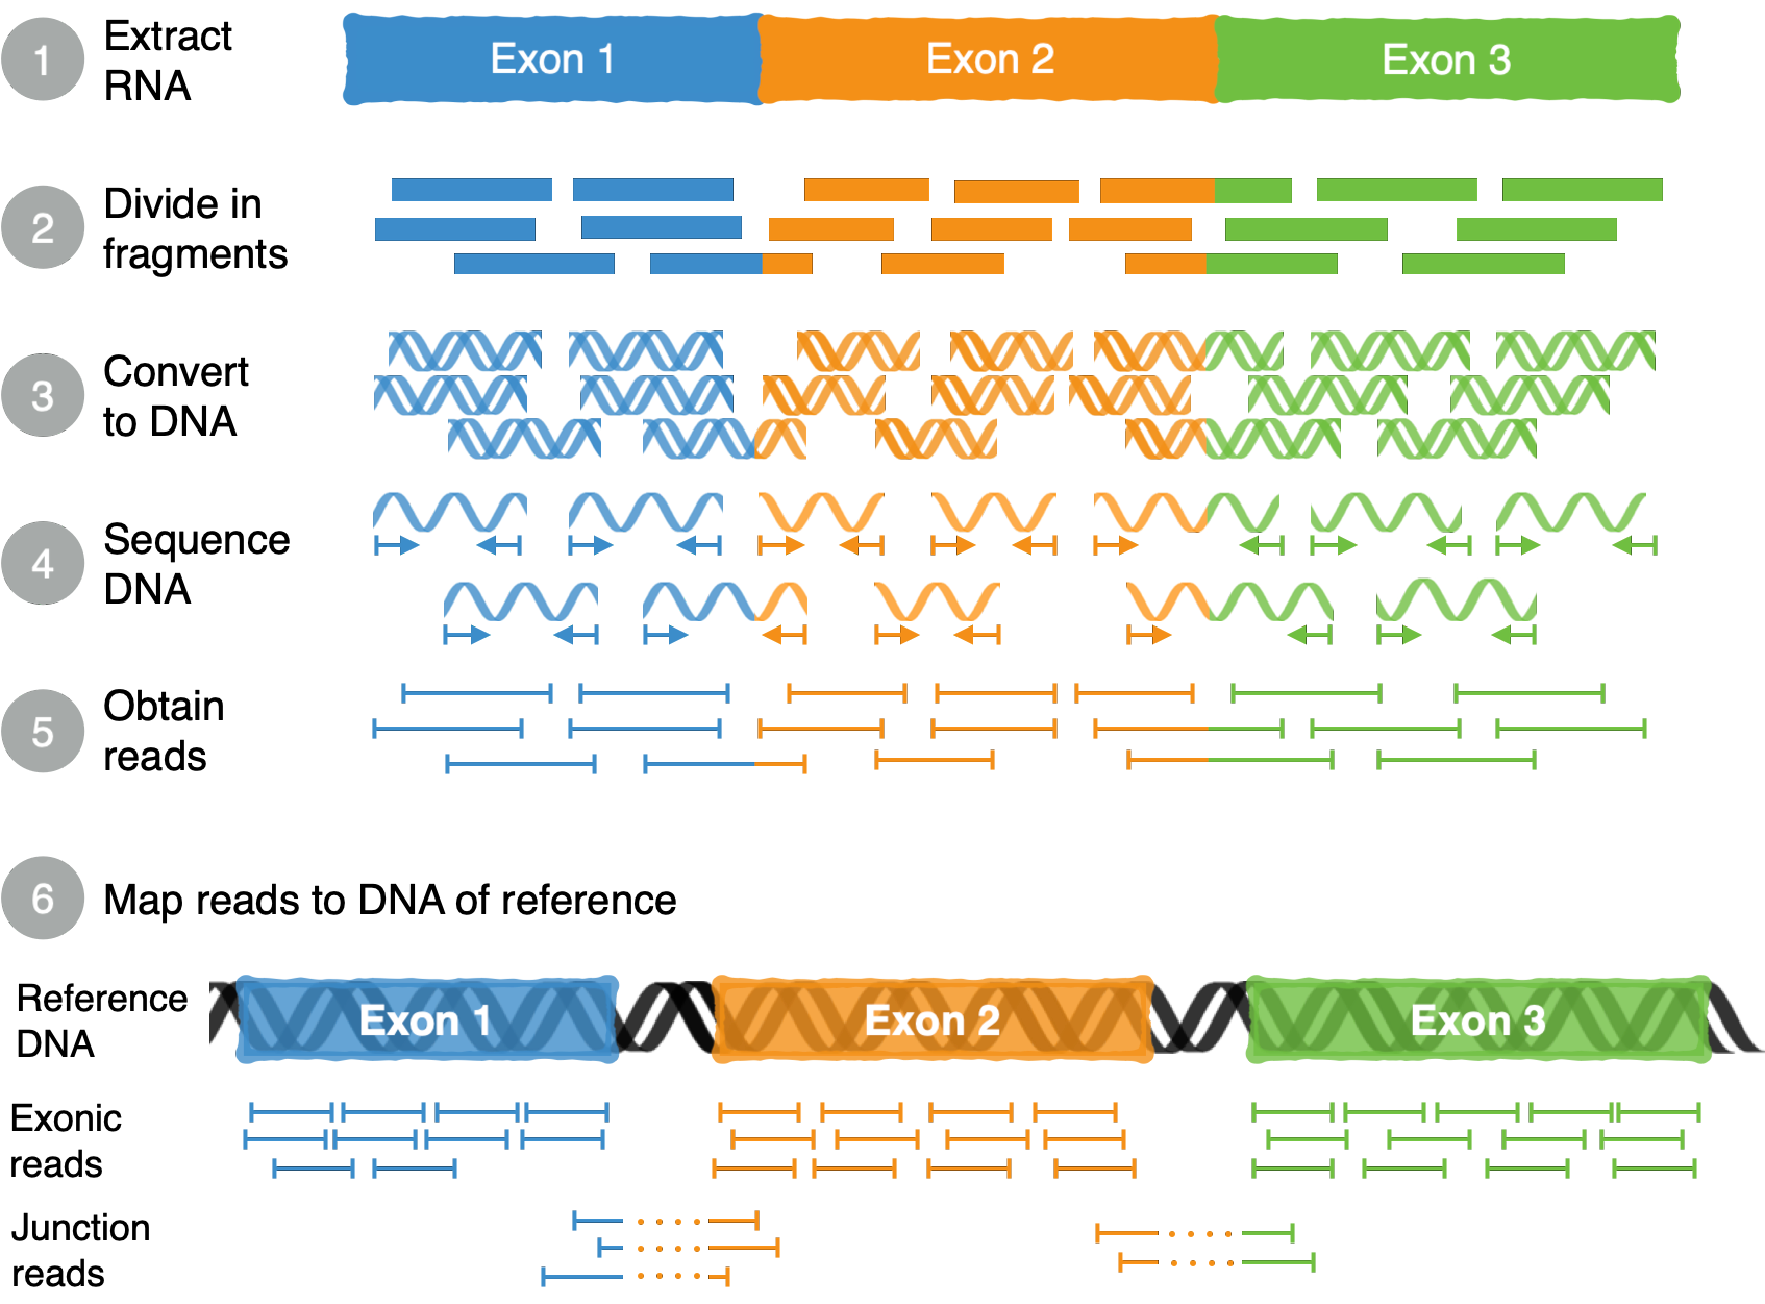
\includegraphics[width=.7\linewidth]{images/intro/rna-seq}
  \caption[RNA sequencing and read mapping]{\textbf{RNA sequencing and read mapping.} RNA is first extracted from a sample (1) and divided into small fragments (2). These fragments are then converted to DNA (3) and sequenced, producing short text strings called reads (4). Finally, these reads are mapped to a DNA of reference (5) allowing to reconstruct the extracted mRNA and identify exon coordinates in the reference DNA.}
  \label{fig:RNAseq}
\end{figure}

%The number of sequencing reads per sample (known as sequencing depth or library size) depends on the intent of the experiment. The quantification of lowly expressed genes, for instance, requires a larger number of reads compared to highly-expressed genes, in order to detect more gene and with higher precision. To assess the sequencing depth required for a certain experiment, we can look at saturation curves.

%Using 3 or more technical replicates allows to reduce external variability. Technical biases may occur, specially when performing multiple batches, as usually done for big sample sizes. To minimise such biases, it is important to use proper controls, randomise sample processing and manage sequencing reads. It is also possible to use batch-correction algorithms, such as ComBat \cite{johnson:2006tj,zhang:2020uq}.

Quality control is an important step in RNA-seq data analysis. Low quality reads, duplicated sequences and overrepresented \emph{k}-mers are some metrics used by FastQC to identify issues with reads from a particular sample that may be mitigated by trimming reads or even discarding samples \cite{andrews:2019vg}. % When performing clustering analyses (after data normalisation), it is expected that reads from replicates cluster together, unless there are potential batch effects or technical biases.

To reconstruct the snapshot at which the RNA was sequenced when using short-read RNA-seq, fragmented reads are compared against a reference genome or transcriptome\footnote{Alternatively, the transcriptome may be reconstructed \emph{de novo} from available transcripts, as usually employed for organisms without any available reference. Given that short reads may be insufficient for this operation, newer technologies based on longer reads are preferentially used.}, allowing to understand where the sequences most likely come from and which features (genes, transcripts, exons, etc.) are more expressed. Unfortunately, some of those sequences match multiple genomic sites, such as reads from repetitive regions, and so are distributed based on empiric evidence and/or randomness. Shorter reads are more prone to mapping to multiple genomic regions and their alignment may prove ambiguous. Such issues can be mitigated by gathering more information on the sequence via paired-end sequencing (i.e., sequencing both ends of the cDNA fragment during RNA-seq) or higher read coverage (i.e., higher number of reads).

% pre-processing (low count removal, technical bias, normalisation)
Based on the number of reads that were aligned to each region of the genome or transcriptome, it is possible to quantify features of interest, e.g., to estimate gene, transcript or exon expression. %To make these counts comparable across samples, they are normalised by transcript length, number of total reads and/or sequencing biases.
These counts are then adjusted to make them comparable across samples and to minimise technical variability, a process known as data normalisation. Afterwards, expression values can be linearly modelled across conditions to identify differentially expressed features \cite{conesa:2016vw}.

Specifically, the study of alternative splicing has been greatly enhanced with the advent of cheaper, high-throughput technologies, since higher read coverage greatly benefits alternative splicing analysis as it captures more fragments from less expressed isoforms \cite{conesa:2016vw}.
One approach to study alternative splicing changes is based on the differential expression of isoforms of a single gene (e.g., CuffDiff2 \cite{trapnell:2013uv}). However, isoform expression estimation based on short reads can be inaccurate because of reads that map to sequences shared by multiple isoforms \cite{conesa:2016vw}.
Other methods based on exon and junction reads specifically identify alterations in events of alternative splicing \cite{conesa:2016vw}: comparing the expression of different exons (differential exon usage, e.g., DEXseq \cite{li:2015tn}), estimating the percentage of alternative sequence inclusion (percent spliced-in, e.g., VAST-TOOLS \cite{irimia:2014wt,tapial:2017ui} and rMATS \cite{shen:2014tk}) or based on graph theory to identify alternative splicing modules (e.g., DiffSplice \cite{hu:2012uw}).
% differential splicing in RNA-Seq data: https://humgenomics.biomedcentral.com/articles/10.1186/1479-7364-8-3

% functional profiling (GSEA, pathway analyses)
% quantification measures
% ncRNAs, long reads, scRNA-seq

% pre-processing (low count removal, technical bias, normalisation)
Transcriptomic studies like those performed using RNA-seq allow to identify altered phenotypes across development stages and pathological subtypes (such as stages of a disease progression), explore the molecular mechanisms underlying a phenotype and pinpoint disease biomarkers. This type of studies can be enhanced by integrating genetic variants, methylation, proteomics and other omics data \cite{chang:2013ww,conesa:2016vw,perez-riverol:2019uk}.

\subsection{Publicly available big data}

The development and economic feasibility of next-generation RNA sequencing lead to a wealth of publicly available sequencing data that can be integrated with available clinical, drug-associated, mutation annotation, methylation and proteomic data. The public availability of these datasets to the research community ensures not only more transparency and reproducibility, but also bigger opportunities to unravel molecular mechanisms, identify more accurate biomarkers and predict novel treatments without spending fortunes from grants to repeat experiments already performed by others, enabling new advances in personalised medicine via data sharing \cite{rockhold:2019ws}. It also means that data can be exploited for other purposes other than those initially intended.

However, the ever-increasing amounts of large-scale data -- \emph{big data} -- require more and more computational resources for their processing and analysis \cite{gauthier:2018ws}, specially when used to train machine learning models. These analyses can be quite time-consuming for non-specialised researches interested in quick biological queries. To satisfy such needs, some projects provide open access to pre-processed data via download (e.g., sequence aligned and normalised data) and apps for data exploration:

\begin{itemize}
	\item \textbf{The Cancer Genome Atlas (TCGA)} with molecular and clinical data for more than 30 human cancer types (e.g., breast cancer and glioma) from more than 10 000 samples \cite{chang:2013ww}. Multiple web apps tap into the data from this behemoth, including TCGASpliceSeq \cite{ryan:2016tm} and Xena Browser \cite{goldman:2020ub}.
	\item \textbf{The Genotype Tissue Expression (GTEx)} project, a repository of gene expression data for more than 40 human tissues, totalling more than 15 000 \emph{post-mortem} samples \cite{lonsdale:2013uo}. The GTEx Portal (\alink{gtexportal.org}) allows to inspect, for instance, the expression values of specific genes and isoforms across multiple tissues.
	\item The \textbf{recount} project has processed RNA-seq data from the Sequencing Read Archive (SRA) \cite{collado-torres:2017uw,wilks:2021uc}.
\end{itemize}

Even with the increasing economic feasibility of RNA-seq, cheaper technologies allow measuring gene expression for larger sample sizes, like in the case of L1000, an inexpensive assay platform where the profiling of 978 transcripts allows to estimate the expression of around 12000 genes via computational inference \cite{subramanian:2017ul}. The development of L1000 was crucial to establish the Connectivity Map (CMap), a collection of almost half a million gene expression signatures derived from chemical and genetic perturbations across multiple cell lines, dosages and timepoints \cite{subramanian:2017ul}. CMap data have been used in multiple contexts, including to identify inhibitors of the stemness signature in multiple TCGA cancer types \cite{malta:2018uj}, to train machine learning models for designing molecules inducing desired transcriptomic changes \cite{mendez-lucio:2020th} and to predict clinically-approved drugs for repurposing as SARS-CoV-2 antiviral agents \cite{le:2021uq}.

To find effective novel treatments, it is important to understand how different cells respond to specific compounds. Multiple drug sensitivity datasets contain compound toxicity data across diverse cell lines, including the NCI-60 \cite{shoemaker:2006wi}, the Cancer Therapeutics Response Portal (CTRP) \cite{seashore-ludlow:2015ws} and the Genomics of Drug Sensitivity in Cancer (GDSC) \cite{yang:2012vk}. Alongside gene expression data for each cell line, these datasets integrate data that allows to, for instance, pinpoint drugs that selectively target malignant cells.
% examples of works made possible thanks to these datasets

Although the number of datasets is getting larger every day, many obstacles render data inaccessible, including lack of standardised formats for storing molecular data and inefficient communication between different platforms \cite{rockhold:2019ws}. Another major hurdle of data dissemination is privacy issues and insufficient anonymisation of clinical data, that can scare away individuals from sharing their personal data in public platforms.

Together with open data, there has also been a push for open access to scientific articles, an important step in disseminating science to everyone, including non-scientists. The publication of pre-prints has also been increasing, allowing for faster research dissemination and for early feedback from peers.

Releasing software as open source is important to allow reproducing published data analysis. Still, code alone may not suffice and the environment changes (e.g., different software versions and operative systems) may lead to unexpected results. To overcome those difficulties, standard tools can be used, like Nextflow to run scalable computational pipelines that may employ Docker containers for reproducibility and portability across machines \cite{di-tommaso:2017vq}.

\subsection{Software development}

% The evolution of software + hardware?
The nature of software has changed throughout the years from simple instructions that calculate Bernoulli numbers, the first published computer program by Ada Lovelace in 1843, to the "foundation for ultra-reliable software design", the on-board flight system that assisted the first moon landing with a crewed mission in 1969, supervised by Margaret Hamilton.

Software plays an important role in society nowadays and scientific research is no exception. For instance, the analysis of RNA-seq data requires specialised tools for quality control, sequence alignment, feature quantification, statistical analyses and visualisation techniques to assist researchers and clinicians in the biological interpretation of their results \cite{conesa:2016vw}. However, many of these specialised tools are developed by scientists with little programming knowledge and may lead to software with structural  issues, e.g., non-user-friendly interfaces, unreproducible results, poorly documented systems, and reliance on deprecated technologies \cite{storer:2017tr,silva:2017wl}.

% Design thinking

To mitigate such issues, scientific software developers can adopt iterative approaches (like agile methodology) that fits the ever-evolving nature of scientific software development. Iterative development facilitates incremental improvement and delivery of stable software iterations by continuously planning and performing small tasks that are evaluated and prioritised based on the project context \cite{storer:2017tr,silva:2017wl,dyba:2009tc}. These development approaches go through a continuous cycle of several steps, including:

\begin{itemize}
    \item{\textbf{Requirement analysis} where we identify stakeholders and their requirements of what the system should do (functional) and that should characterise the system (non-functional; e.g., modular, reliable, secure, easy-to-use and scalable) \cite{silva:2017wl,hewitt:2019uj}. The initial requirements of a system tend to (and should) be of higher-level, but increase in complexity as the project advances: in simpler terms, a first version of the software should be simple and improved upon to get more features over time \cite{silva:2017wl,kanat-alexander:2012ve}.}
    \item{\textbf{Design} concerns with the technologies to use during software development (e.g., frameworks for web app development and cloud hosting solutions for distribution), as well as the proper implementation of new features in the current software iteration or the integration with other programs via standard application programming interfaces (APIs), for instance. Good software design should allow to extend current functionality with as few changes to the core of the program as possible.}
	\item{\textbf{Development}, such as code structuring, feature implementation, bug fixing and code optimisation.}
	\begin{itemize}
	    \item Version control systems (e.g., git) track changes to files in a project, allow to easily integrate code from different developers and compare files across diffterent versions \cite{silva:2017wl,ford:2021ub}.
		\item Kanban-like boards allow to visualise and manage the project workflow, where features and bugs can be commented on and tracked \cite{silva:2017wl,hewitt:2019uj}.
		\item Comprehensive documentation (tutorials, manuals, wikis, inline source code comments, etc.) is crucial to showcase the program and explain how features work via functions' description and examples to end-users and developers alike and can be written in plain text, Markdown and other common file formats \cite{storer:2017tr,silva:2017wl,kanat-alexander:2012ve,ford:2021ub}. For development purposes, good documentation facilitates the maintenance and reusability of the program. Multiple tools automatically generate documentation from inline source code comments for different programming languages that can be automated, including roxygen2 for R \cite{wickham:2021wt} and Sphinx for Python \cite{silva:2017wl,hewitt:2019uj}.
	\end{itemize}
	\item{\textbf{Testing} via unit tests, usability tests, performance tests, integration tests and security tests. Testing should be performed in multiple environments (e.g., different versions of programming languages, dependencies, operating systems and web browsers) \cite{silva:2017wl,kanat-alexander:2012ve,ford:2021ub}. The portion of the code covered by unit tests (written to check particular parts of code return the expected output when run) can be evaluated using code coverage tools such as CodeCov, allowing to understand how much of the code is being tested \cite{hewitt:2019uj}.}
	\item \textbf{Software distribution (deployment)} is related with the release of program iterations to the hands of end-users: the easier it is to deploy, the faster new iterations can be released with new features and bug fixes \cite{ford:2021ub}.
	\begin{itemize}
		\item Software can be distributed as web-browser-based applications (web apps) or desktop apps. Containerisation (e.g., via Docker) also helps distributing complex software and its dependencies in an easier way. There are also many available repositories that allow to store code and/or compiled programs (GitHub to store git projects, DockerHub for Docker images, Bioconductor for bioinformatic R packages \cite{huber:2015wt} and CRAN for generic R packages).
		\item When distributing code and/or programs, licensing must be defined since the first general release to avoid code misuse by third parties \cite{silva:2017wl}. Different types of licenses can be chosen, allowing to decide whether the program can be modified, redistributed, used for commercial purposes and whether there are special conditions (e.g., any code derivation must be open-source and modifications must retain same license) \cite{silva:2017wl}.
		\item User feedback via bug reports and feature requests should be collected and considered for future  iterations.
	\end{itemize}
\end{itemize}

To facilitate continuous iterations, some steps can be automated using continuous integration (CI) tools, allowing to compile, run, test, deploy and document software. Those steps can then run in a multitude of environments whenever new changes are integrated in the code or at a regular interval (e.g., weekly) to ensure compatibility of the current version with newer versions of external dependencies. Automation tools are crucial to quickly detect issues in a multitude of reproducible contexts and to promote code quality, testability, integration and continuous feedback \cite{silva:2017wl,hewitt:2019uj,ford:2021ub,storer:2017tr}.

Many popular CI tools, like Travis-CI, GitHub Actions and AppVeyor, can be used for free in open-source projects. This approach promotes software quality by allowing peer-reviewing the code, reusing parts, fixing bugs, extending features and collaborating with external developers \cite{silva:2017wl,hewitt:2019uj}, as well as it facilitates analysis transparency and reproducibility \cite{silva:2017wl}. Moreover, it has educational value, allowing others to learn from the developed code, implemented solutions and project organisation \cite{hewitt:2019uj}.

%Open-source bioinformatic R packages are supported by Bioconductor and its community \cite{huber:2015wt}, facilitating the distribution of R packages and Docker images that allow easy access to their most popular R packages. Bioconductor also hosts packages that make use of the Shiny framework to create web apps from R \cite{chang:2021ul}.

\subsection{Web apps and graphical user interfaces}

The advent and popularisation of the Internet made software easier to distribute by simply allowing to download apps or use web browsers to directly present web apps. Web apps follow a client-server architecture usually composed by three layers:
\begin{itemize}
	\item \textbf{Presentation layer} is the user interface locally rendered by the user's web browser based on standard web technologies: HTML, CSS and JavaScript.
	\item \textbf{Database layer} contains app-associated data such as user login details. The database may be stored remotely (most commonly using a MySQL, PostgreSQL, MariaDB or MongoDB server) or in the user's computer.
	\item \textbf{Application layer}, the core logic of the application. The application layer can be run in its own remote server or in the same server as the database layer based on Python, Java, PHP or Perl. However, simpler web apps may opt for running the application layer as part of the presentation layer, thus using local resources.
\end{itemize}

Specially used in business intelligence, dashboards are a common type of web app that allow interactive data analysis to explore key performance indicators (KPI). Dashboards have increasingly been the subject of health care research, from monitoring medical equipment performance \cite{iadanza:2019tj} and assessing surgical performance \cite{baghdadi:2021uc} to predicting high-risk patients for primary palliative care \cite{tan:2020tu}. Inspired by such dashboards, tools to explore and analyse bioinformatic data are also available, including to explore gene expression from user-provided data or from public datasets (e.g., \cite{reyes:2019ud,cardoso-moreira:2019wd}).

To provide effective dashboards, good practices in data visualisation are paramount for intuitive communication of complex results \cite{tidwell:2019tf}. By introducing interactivity, the user can explore and manipulate the represented data, allowing greater flexibility to analyse and scrutinise the results relative to a comparable static plot and to obtain greater information insight by scrolling, zooming and drilling down into specific points \cite{tidwell:2019tf}.

Another vital aspect of any app is its interface, no matter whether graphical or command-line based. User-centred interfaces assist users achieving their goals by considering the program's audience, including their intents while using the program, the expectations on how to achieve them, familiarity with the vocabulary employed, computing skills and experience using similar software. Research on user interface design focuses beyond computing systems and covers human cognition, behaviour analysis and psychology \cite{silva:2017wl,hewitt:2019uj,tidwell:2019tf,alves:2020vu}. Interfaces can be evaluated and improved by asking for and listening to user feedback or by performing usability testing \cite{tidwell:2019tf}.

Unfortunately, there is a lack of documentation on creating proper visual interfaces for bioinformatic apps. Even so, combining the concepts behind proper software development with dashboard design, big data visualisation and state-of-the-art transcriptomic analysis in freely available, open-source tools allows us to create potentially useful and (hopefully) popular web apps for sharing data insights with collaborators and even the whole scientific community.

\subsection{R programming language}

The work presented in this thesis was mostly developed using R \cite{r-core-team:2021wf}. R is a programming language with a strong foundation in statistics and includes native support for data manipulation, clustering, survival analysis, principal component analysis, linear modelling and classical statistical tests, such as Mann-Whitney U, Kruskal–Wallis and Fligner–Killeen tests \cite{r-core-team:2021wf,therneau:2000tk}. We also used RStudio (\alink{rstudio.com}), a popular integrated development environment (IDE), to assist using R for data analysis and package development.

Besides the built-in functions, R is extendable with open-source packages from multiple repositories, e.g., CRAN for generic R packages and Bioconductor for bioinformatic R packages \cite{huber:2015wt}. We used packages from such repositories to:

\begin{itemize}
	\item perform bioinformatic analyses, including differential gene expression (\texttt{limma} \cite{ritchie:2015tm} and \texttt{edgeR} \cite{robinson:2010wx});
	\item create interactive data visualisations based on \texttt{ggplot2} \cite{wickham:2016aa} for standard R plots and \texttt{highcharter} \cite{kunst:2022aa} for interactive JavaScript plots;
	\item design web apps using the \texttt{shiny} \cite{chang:2021ul} framework;
	\item integrate C++ in R with \texttt{Rcpp} \cite{eddelbuettel:2018aa}, a more efficient and low-level programming language, allowing to speed up computationally-intensive tasks;
	\item profile time and memory to pinpoint bottlenecks that need improvement by using \texttt{profvis} \cite{chang:2020aa} and \texttt{microbenchmark} \cite{mersmann:2021aa};
	\item develop R packages with \texttt{devtools} \cite{wickham:2021aa} and write their documentation using \texttt{roxygen2} \cite{wickham:2022aa}.
\end{itemize}

To facilitate the use of the code in this thesis, our programs are distributed as open-source in GitHub and Bioconductor. Moreover, our tools were encapsulated with their dependencies in Docker images, making them quick to set up in any machine and easy-to-use in high-performance computing (HPC) environments. We also used these Docker images to deploy our tools as free web apps.

The LaTeX code to compile this PhD thesis is open-source and can be found at \alink{github.com/nuno-agostinho/phd-thesis}.


% !TEX root = ../PhD Thesis.tex
\chapter{Objectives}

The aim of the scientific work discussed in this thesis is to develop transcriptomic apps with graphical and command-line interfaces to retrieve and analyse publicly available transcriptomic data from popular repositories, such as TCGA \cite{chang:2013ww}, GTEx \cite{lonsdale:2013uo}, recount2 \cite{collado-torres:2017uw} and CMap \cite{subramanian:2017ul}. Besides, we intend their graphical interfaces to be intuitive, flexible and deployed online as web apps, so that they are used by a wide range of researchers. We think that bridging the gap between big data and researchers with basic computational skills will inspire them to learn more about bioinformatic analyses and thereby potentiate their ability to extract novel biological insights from genome-wide molecular information.

Alternative splicing is involved in multiple cellular processes, with its deregulation being linked to diverse pathologies. The use of pre-processed alternative splicing data from public repositories exempts researchers from storing and processing large raw files that require expensive computational resources. However, until 2018, no tools interactively fetched those public data and allowed their analyses using user-defined sample groups based on associated metadata. Thus, there was a need to develop a program with a graphical interface that allows to quantify, analyse and visualise publicly available alternative splicing data. We used the R programming language to create psichomics \cite{saraiva-agostinho:2018uq,saraiva-agostinho:2020wz}, an open-source R package with a Shiny-based web interface that automatically downloads biological data from TCGA \cite{chang:2013ww}, GTEx \cite{lonsdale:2013uo} and recount2 \cite{collado-torres:2017uw}. By making use of popular R packages like \texttt{edgeR} \cite{robinson:2010wx} and \texttt{limma} \cite{ritchie:2015tm} for gene expression analysis, psichomics interactively performs dimensionality reduction, differential splicing and gene expression and survival analyses with incorporation of molecular and clinical features. % We benchmarked psichomics to check its speed and memory efficiency relative to different data sizes, but also if their quantifications are comparable to the standard alternative splicing quantification tools.

% Based on the work I developed during my MSc thesis \cite{saraiva-agostinho:2016vw}, I continued working on psichomics \cite{saraiva-agostinho:2018uq,saraiva-agostinho:2020wz}, an alternative splicing quantification, analysis and visualisation R package for pre-processed human data from TCGA \cite{chang:2013ww}. During my PhD, psichomics was extended to support more data sources (including GTEx \cite{lonsdale:2013uo}, recount2 \cite{collado-torres:2017uw} and user-provided data), analyse gene expression and support alternative splicing quantification for 14 different species, among other features.

CMap is a public database containing millions of gene expression changes in response to induced molecular and pharmacological perturbations \cite{subramanian:2017ul}. Comparing differential gene expression profiles with those from CMap allows to infer putative molecular causes for the observed differences, as well as compounds that may promote or revert those changes. To facilitate this approach, we strived to build a program to identify potentially causal molecular perturbations by comparing user-provided differential gene expression results with those from CMap, using correlation and gene set enrichment scores. Moreover, the program should also use gene expression/drug sensitivity associations from public databases to identify compounds that may target the phenotypes associated with the user-provided differential expression profiles. We used R/Shiny to create cTRAP, an R package with graphical interface functions to assist users performing the aforementioned features.

% This can be accomplished using user-friendly tools available from the CMap and LINCS Unified Environment (\mbox{\alink{clue.io}}) \cite{subramanian:2017ul}. However, \alink{clue.io} limits the maximum number of input genes for CMap queries, is difficult to automate for downstream analyses and cannot be run using local computing resources. Furthermore, \alink{clue.io} does not currently integrate with drug sensitivity datasets to further assist in pinpointing compounds that selectively target cells \cite{almeida:2019wh}.

%I led the development of cTRAP, an R package to identify candidate causal perturbations from differential gene expression data, as well as predict compounds that may promote or revert them. cTRAP also allows to list putative targeting drugs based on drug sensitivity datasets and includes a GSEA-based analysis of molecular descriptors for compounds from NCI-60 and CMap.

Both psichomics and cTRAP feature web-based graphical interfaces to assist users interactively performing most of their functions following easy steps, properly detailed in online tutorials that are constantly updated according to user feedback. To make Shiny apps accessible via a web browser, we intended to build an open-source and portable codebase to easily deploy web apps using our own custom server. Therefore, I led the development of an app server based on Docker and ShinyProxy to deploy psichomics, cTRAP and multiple R packages as web apps -- including other programs built by my lab colleagues in the lab (voyAGEr, betAS and scStudio). I kindly invite you to pause, sit back and relax, visit our website at \alink{compbio.imm.medicina.ulisboa.pt}, wander through the web apps there and enjoy the journey. The landing page is a gallery of work from our lab that I am deeply proud to support.

%% !TEX root = ../PhD Thesis.tex
\chapter{Materials and Methods}

\section{R programming language}

\subsection{Shiny}

Interactive plots via highcharter

\subsection{Bioconductor}

Packages in Bioconductor can only depend on CRAN or Bioconductor packages

Two releases per year

\section{Datasets}

TCGA
GTEX
SRA/recount2
CMap

Alternative splicing annotation

Alternative splicing quantification

\section{Data analyses}

Gene expression normalisation and filtering

Differential gene expression

Differential alternative splicing

PCA + survival analyses

\section{Software development}

GitHub

\subsection{Documentation}

Function documentation

pkgdown

Vignettes / tutorials

\subsection{Unit testing}

\subsection{Continuous testing}

GitHub Actions

Docker + Docker Hub + Docker Compose

Nextflow

\subsection{Benchmarking}


% !TEX root = ../PhD Thesis.tex
\chapter{psichomics}

\begin{figure}[!b]
  \vspace*{-.5cm}
  \includegraphics[width=.93\textwidth]{images/psichomics/screenshot}
  \centering
  \vspace*{-.5cm}
  \caption[psichomics screenshot]{\textbf{psichomics screenshot.} TCGA breast cancer splicing analysis (28 Jan 2020).}
  \label{fig:psichomics-screenshot}
\end{figure}

After finishing the first year of my Masters in Informatics, I was looking for a challenging thesis where I could apply all that I learned into a bioinformatics project. While looking for computational biology groups, I found out about Nuno Morais lab, a research group interested in studying transcriptomics in disease.

Nuno made me aware of the need for graphical, interactive tools to allow non-experts to analyse and visualise splicing from processed big datasets. I loved the idea and started exploring ways of going from concept to reality. After toying with multiple frameworks and programming languages, I decided to stick with the R statistical language and the Shiny web app framework \cite{chang:2021ul} that helped me to kick-start what would be later known as psichomics (\shortref{fig:psichomics-screenshot}).

psichomics was first available in 2016 via Bioconductor to quantify, analyse and visualise human alternative splicing using TCGA data \cite{chang:2013ww}. Later on, I started my PhD in the same lab and continued my work on psichomics. Nowadays, the tool also analyses gene expression and alternative splicing based on user-provided or public transcriptomic data, including those from GTEx \cite{lonsdale:2013uo} and recount2 \cite{collado-torres:2017uw} (\shortref{tab:psichomics}).

% Following an invitation from Springer Methods, I also prepared a book chapter on using psichomics to analyse alternative splicing in stem cell differentiation \cite{saraiva-agostinho:2020ue}.

\begin{table}[!ht]
\small
\caption[Major psichomics milestones]{\textbf{Major milestones of psichomics.}}
\label{tab:psichomics}
\begin{tabularx}{\textwidth}{ l r l }
\toprule
\textbf{Version} & \textbf{Release date} & \textbf{Main features} \\
\midrule
1.0  & 18 Oct 2016 & Quantify and analyse alternative splicing from TCGA data\parnote{Bioconductor release.} \\
1.0.8  & 18 Feb 2017 & Analyse GTEx data \\
1.4  & 31 Oct 2017 & Analyse gene expression from TCGA and GTEx data \\
1.4.2  & 19 Dec 2017 & Support human genome assembly hg38 \\
1.4.3  & 13 Jan 2018 & Faster alternative splicing quantification using Rcpp/C++ \\
1.6.1  &  5 Jul 2018 & Analyse recount2 and user-provided data \\
\rowcolor{lightgray}
       &  2 Oct 2018 & psichomics' original article \cite{saraiva-agostinho:2018uq} is published online \\
1.8.2  & 27 Mar 2019 & Add list of RNA-binding proteins \cite{sebestyen:2016tr} \\
\rowcolor{lightgray}
       & 21 Jan 2020 & psichomics' book chapter \cite{saraiva-agostinho:2020wz} is published online \\
1.12.1 & 29 Jan 2020 & Display visual diagrams of alternative splicing events \\
1.14.2 & 11 Aug 2020 & Load VAST-TOOLS output\parnote{First time supporting intron retention events (psichomics does not quantify intron retention). More information in \fullref{sec:psi-quantification}.} and more data formats \\
1.18.6 & 4 Oct 2021  & Add web server support (optimised to run in ShinyProxy)\parnote{First version available online.} \\
1.20 & 28 Oct 2021 & Support alternative splicing annotation for 14 species\parnote{Alternative splicing annotations for multiple species are available on-demand based on VAST-TOOLS annotation. \shortref{tab:as-annot} lists all supported species/assemblies. Custom alternative splicing annotations can also be imported.} \\
\bottomrule
\end{tabularx}
\parnotes
\end{table}

Following many user requests, support for non-human data analysis was added with alternative splicing annotations for 14 species (including mouse, fruit fly, frog, and \emph{Arabidopsis thaliana}). These annotations were published in Bioconductor and are based on those provided by alternative splicing quantification tool VAST-TOOLS \cite{irimia:2014wt,tapial:2017ui}. Other improvements include support for loading VAST-TOOLS output tables, thus allowing to analyse intron retention events. However, I feel like it took until 2021 to fully realise psichomics' potential -- when it finally went online\footnote{More information in \fullref{chap:app-server}.}.

Following the publication of the first article describing psichomics in 2018 \cite{saraiva-agostinho:2018uq}, we were invited to write a methodological book chapter published in 2020 \cite{saraiva-agostinho:2020wz}. Both publications were written by me (as the first and a co-corresponding author) and Nuno Morais. The content of those publications, along with some content from my MSc Thesis \cite{saraiva-agostinho:2016vw}, greatly inspired this chapter.

\section{Background}

%Alternative splicing fosters transcriptome diversity in eukaryotes through the processing of pre-mRNAs from the same gene into distinct transcripts that may encode for proteins with different functions \cite{kelemen:2013tc,paronetto:2016vw}. Alternative splicing is involved in multiple cellular processes, such as apoptosis and autophagy regulation \cite{kelemen:2013tc,paronetto:2016vw}, and is especially prevalent in humans, where around 93\% of genes display alternatively spliced transcripts whose regulation may differ across tissues and developmental stages \cite{paronetto:2016vw,wang:2008wa,barbosa-morais:2012ut}. Consistently, alternative splicing dysregulation has been linked with cancer, neurodegeneration and other diseases \cite{paronetto:2016vw,oltean:2014vm,gallego-paez:2017wc}. For instance, splicing alterations mediated by the key regulator SRSF1 may impact multiple hallmarks of cancer, such as resistance to apoptosis and tissue invasion \cite{oltean:2014vm}.

The relevance of alternative splicing changes in physiological and disease conditions, along with the increasing economic feasibility of RNA-seq, has progressively driven transcriptome-wide alternative splicing studies \cite{wang:2008wa,tsai:2015ve,danan-gotthold:2015ut,chhibber:2017wm,climente-gonzalez:2017uj} and promoted large consortium efforts to assemble publicly accessible splicing data. Such efforts include TCGA that catalogues clinical and molecular profiling data from multiple human tumours \cite{chang:2013ww}; GTEx that focuses on profiling normal human multi-tissue data \cite{lonsdale:2013uo}; and the recount2 project, a resource of processed RNA-seq data for over 2000 studies, mostly from the Sequence Read Archive (SRA) \cite{collado-torres:2017uw}.

Among the openly available processed data from those public projects, counts of RNA-seq reads aligned to exon-exon junctions may be exploited for alternative splicing quantification and further analysis. Indeed, the ability to couple proper differential splicing analysis with, for instance, gene expression, protein domain annotation, clinical information or literature-based evidence enables researchers to extract, from those comprehensive public datasets, valuable insights into the role of alternative splicing in physiological and pathological contexts, as well as putative splicing-associated prognostic factors and therapeutic targets \cite{tsai:2015ve,danan-gotthold:2015ut,chhibber:2017wm,climente-gonzalez:2017uj,anczukow:2015vl}.

Several tools are currently available to quantify, analyse and visualise alternative splicing data. Some analyse alternative splicing based on the commonly-employed and intuitive proportion of reads aligned to splice junctions supporting the inclusion isoform, known as Percent Spliced-In or PSI \cite{wang:2008wa}. Examples of such tools are AltAnalyze \cite{emig:2010ws}, MISO \cite{katz:2010tj}, SpliceSeq \cite{ryan:2012ts}, VAST-TOOLS \cite{irimia:2014wt}, rMATS \cite{shen:2014tk}, SUPPA \cite{alamancos:2015vc} and Whippet \cite{sterne-weiler:2018tk}. Regardless of their quantification metric, alternative splicing analysis tools had at least one of the following shortcomings in 2018:

\begin{enumerate}
	\item Lack of support for imputing pre-processed data (e.g., splice junction read counts), leading to redundant, time-consuming RNA-seq read alignment and exon-exon junction detection, preceding alternative splicing quantification when exon-exon junction quantification is already available (e.g., when analysing TCGA, GTEx or recount2 data).
	\item Limited set of statistical options for differential splicing analysis, mostly relying on median-based non-parametric tests and restricted to pairwise comparisons.
	\item No incorporation of molecular or clinical information enabling analyses that reflect factorial designs or test linear models, for example. This is particularly limiting in the exploration of clinical datasets where, for instance, survival analyses permit assessing the potential prognostic value of alternative splicing events.
	\item No support for transcriptome-wide filtering and sub-setting of events, based on common features or the outcome of statistical analyses, for interactive exploration of individual events of interest.
	\item No user-friendly interactive graphical interface neither support for customisable statistical plots.
\end{enumerate}

Using available pre-processed splice junction read counts from big data repositories exempts researchers from storing and processing large raw files that require expensive computational resources. To our knowledge, until 2018 no tool performed transcriptome-wide alternative splicing analysis using splice junction read counts from publicly available RNA-seq datasets (e.g., from TCGA, GTEx and recount2) with the option to easily compare them with user-provided groups interactively created based on sample metadata. For instance, jSplice \cite{christinat:2016ui} and DIEGO \cite{doose:2018uv} do quantify alternative splicing from junction read counts but the user needs to manually convert such counts into a file format accepted by those programs. Moreover, none of those tools support survival analysis, exploratory and differential analyses of gene expression, or tests for association between gene expression levels and/or alternative splicing quantification changes.

To offer a comprehensive pipeline that integrates all the aforementioned features through both a command-line and an easy-to-use graphical interface, we have developed psichomics, an R package to quantify, analyse and visualise alternative splicing and gene expression data using TCGA, GTEx, recount2 and/or user-provided data. Our tool interactively performs dimensionality reduction, differential splicing and gene expression and survival analyses with incorporation of molecular and clinical features.

% We successfully employed psichomics to analyse stage I breast cancer TCGA data and identified alternative splicing events with putative prognostic value.

psichomics is available online as a web app at \alink{compbio.imm.medicina.ulisboa.pt/psichomics}, but can also be locally installed using Bioconductor (\alink{bioconductor.org/packages/psichomics}) or Docker (\dockerlink{nunoagostinho/psichomics}). The source code of psichomics is available at \alink{github.com/nuno-agostinho/psichomics}.

\section{Materials and methods}

psichomics allows to automatically process data (provided by the user or automatically downloaded from TCGA, GTEX and recount2), quantify alternative splicing, normalise and filter gene expression data and perform downstream analyses, including dimensionality reduction, differential expression/splicing analysis, correlation analysis, survival analysis and annotation of genes, transcripts and proteins (\shortref{fig:psichomics-workflow}).

\begin{figure}[!ht]
  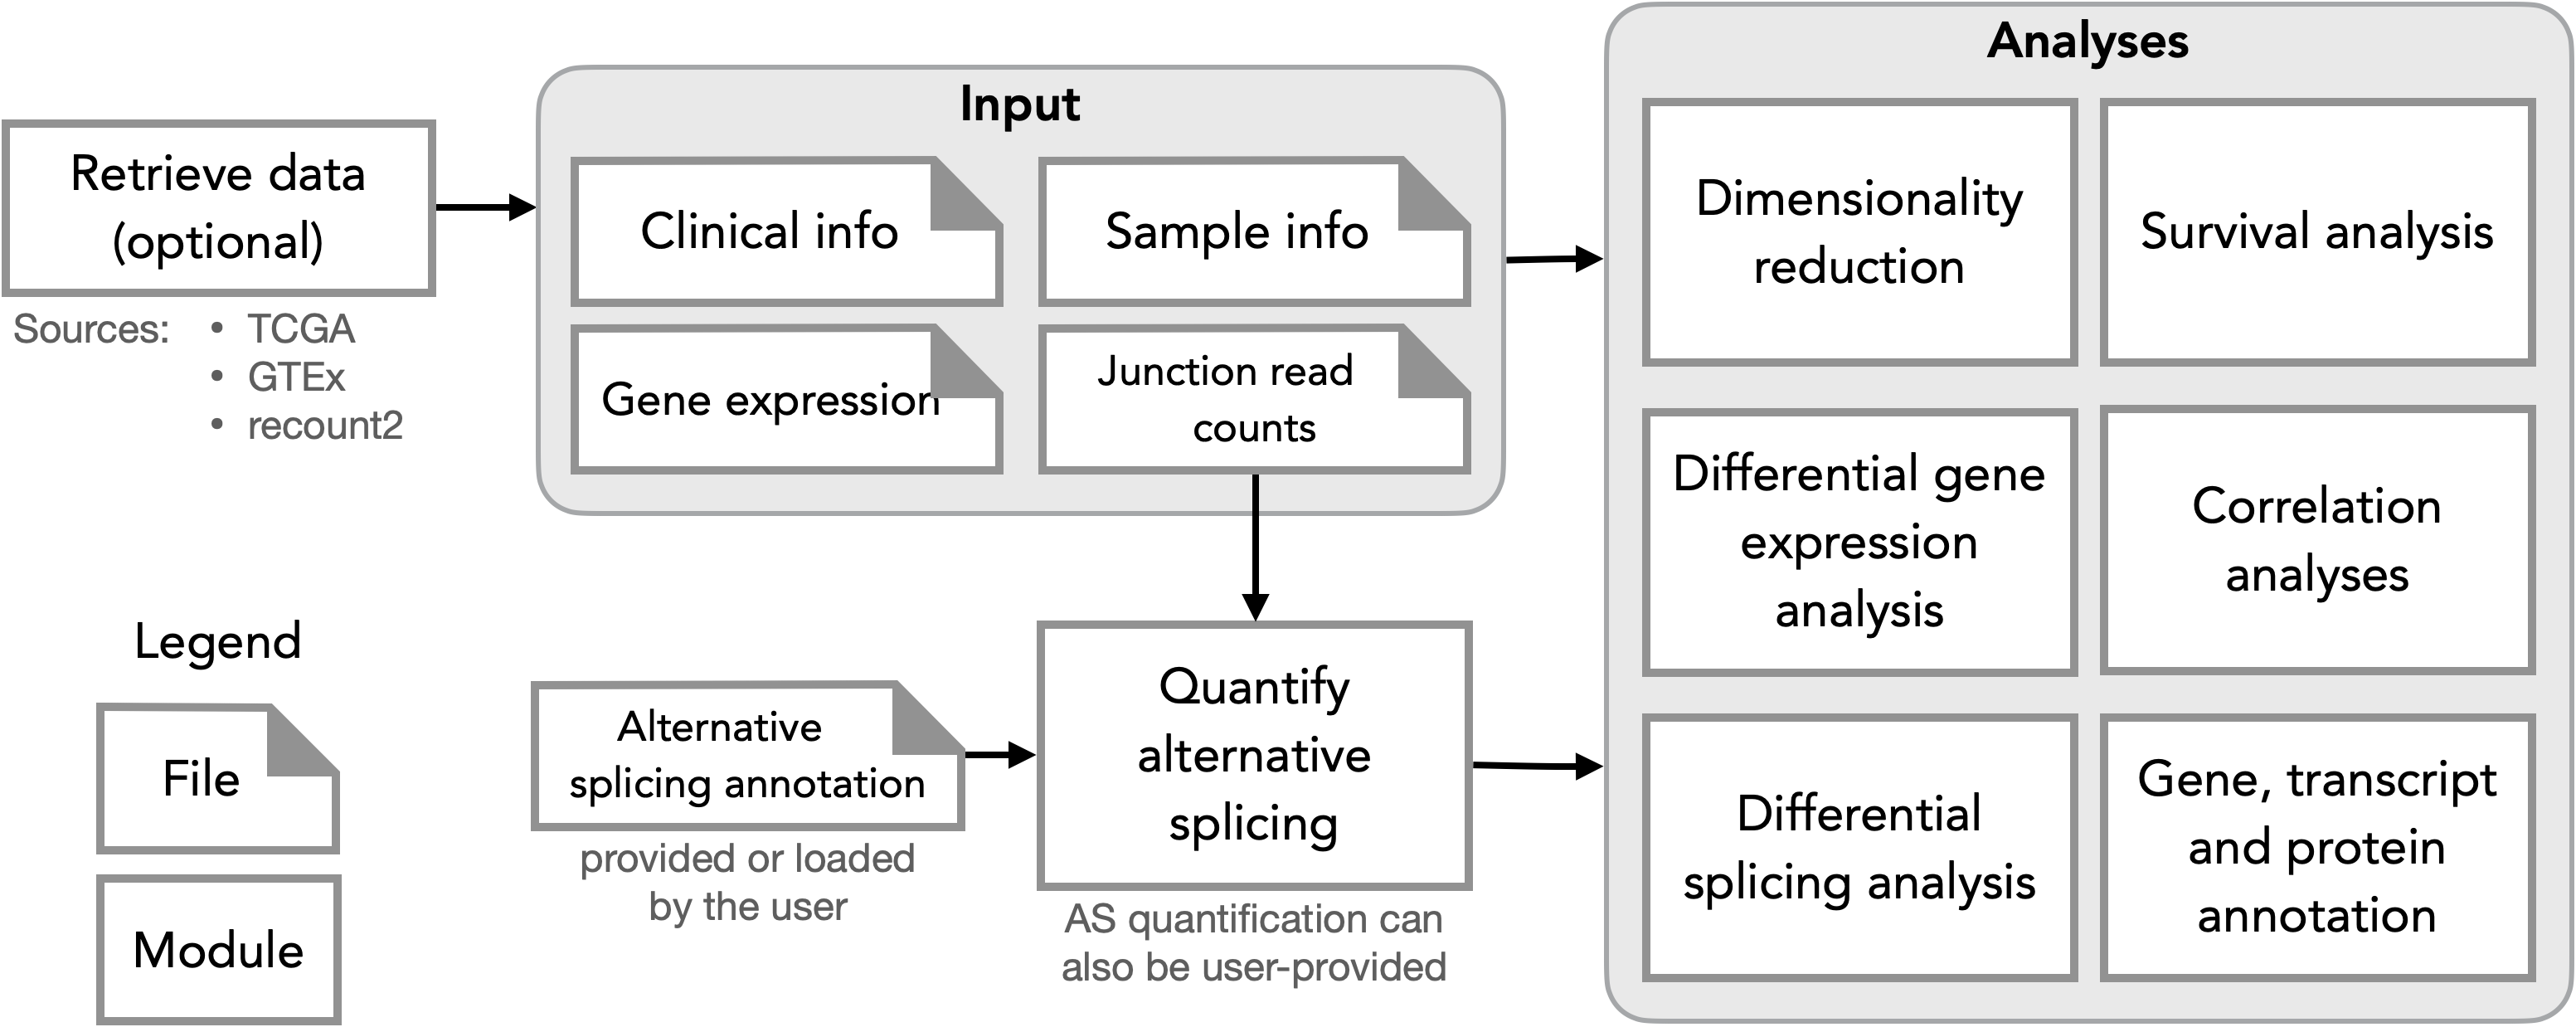
\includegraphics[width=.94\textwidth]{images/psichomics/workflow}
  \centering
  \caption[psichomics workflow]{\textbf{psichomics workflow.} The user can provide their own input data or load data from TCGA, GTEx or recount2 to normalise gene expression data and quantify alternative splicing for downstream analyses.}
  \label{fig:psichomics-workflow}
\end{figure}

% TODO: add new symbol for a group of files to make it more intuitive to understand why there are multiple R files for the same data source
\begin{figure}[!ht]
  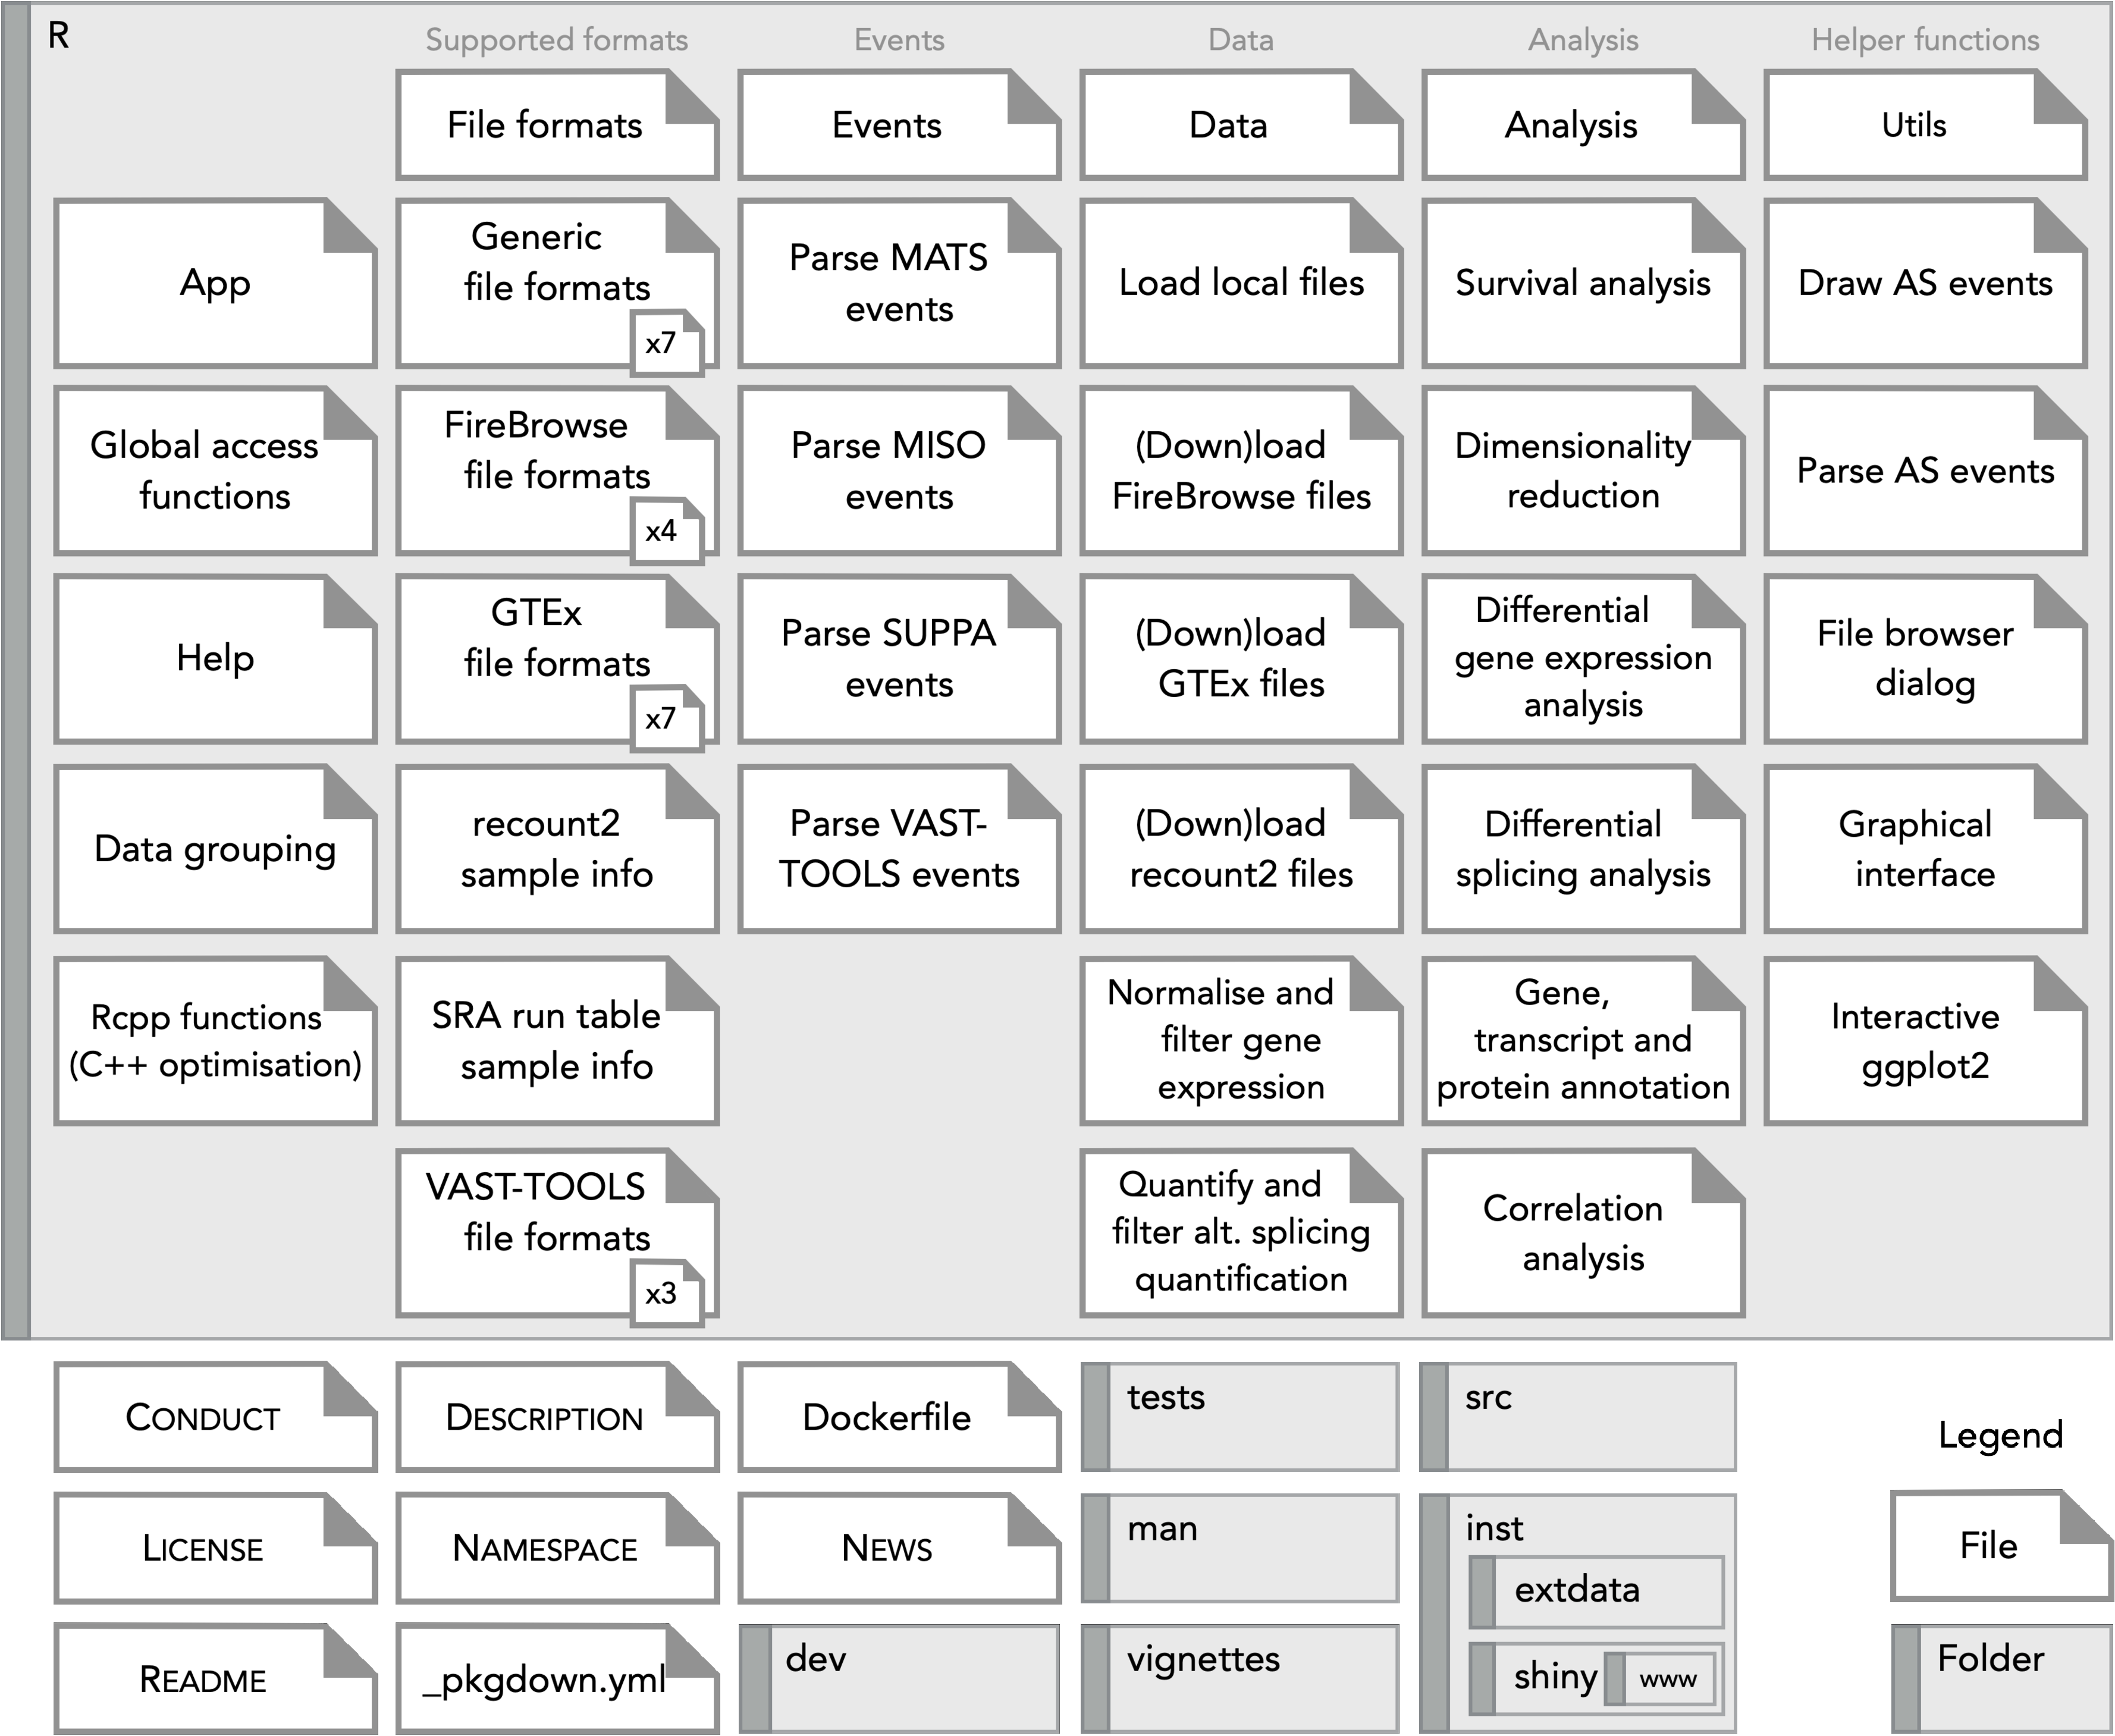
\includegraphics[width=\textwidth]{images/psichomics/file-structure}
  \centering
  \caption[psichomics file structure]{\textbf{Visual representation of psichomics' file structure.} psichomics is a modular program where, for instance, functions specific for different data sources and analyses can be found in different files. As usual for R packages, the \texttt{R} folder is the heart of the code and contains the main R scripts that define the logic and interface of the app. \texttt{dev} is a non-standard folder in R packages used to store supporting scripts (e.g., test workflows); its contents are not included when building the R package.}
  \label{fig:psichomics-file-structure}
\end{figure}

The tool was designed as a modular R package to be easily modified and extended (\shortref{fig:psichomics-file-structure}), including modules for automatic data retrieval from multiple sources, parsing and standardisation of alternative splicing event identifiers from different programs and a variety of data analysis methodologies.

psichomics can load splice junction read count data provided by the user or from external sources, followed by the quantification of alternative splicing (in case no pre-computed quantification is loaded) and subsequent analyses. Alternative splicing quantification is computed based on RNA-seq reads that align to exon-exon junctions and the genomic coordinates (annotation) of alternative splicing events. The proportion of reads aligned to junctions that support the inclusion isoform, known as the Percent Spliced-In or PSI \cite{wang:2008wa}, was the chosen quantification metric.

\subsection{Data retrieval}

Exon-exon junction and gene expression quantifications (obtained from pre-processed RNA-seq data), clinical data and sample metadata are accessible through FireBrowse's web application program interface (API) for TCGA data retrieval (\alink{firebrowse.org/api-docs}). The FireBrowse API is used in psichomics to automatically download TCGA data according to the user-selected tumour type(s) as tab-delimited files within compressed folders, whose contents are subsequently loaded with minimal user interaction. GTEx data are automatically downloaded via the GTEx data portal (\alink{gtexportal.org}) and select SRA project data via recount2 \cite{collado-torres:2017uw}. Other SRA projects and user-provided files may also be loaded in appropriate formats (\shortref{tab:psichomics-file-formats}), allowing for subsequent alternative splicing analysis\footnote{Refer to tutorial at \alink{nuno-agostinho.github.io/psichomics/articles/custom_data}.}.

\begin{table}[!ht]
\parnotereset
\small
\caption[Supported file formats in psichomics based on data source]{\textbf{Supported file formats in psichomics based on data source.}}
\label{tab:psichomics-file-formats}
\begin{tabularx}{\textwidth}{ l X X X X X }
\toprule
{\textbf{Source}} & {\textbf{Sample information}} & {\textbf{Subject information}} & {\textbf{Gene expression}} & {\textbf{Exon junction quantification}} & {\textbf{Alternative splicing quantification}} \\
\toprule
\textbf{SRA Run Selector} & Yes &     &     &     &     \\
\midrule
\textbf{STAR}             &     &     & Yes & Yes &     \\
\midrule
\textbf{VAST-TOOLS}       &     &     & Yes &     & Yes \\
\midrule
\textbf{TCGA/FireBrowse}  & Yes & Yes & Yes & Yes &     \\
\midrule
\textbf{SRA/recount2}     & Yes & Yes & Yes & Yes &    \\
\midrule
\textbf{GTEx}             & Yes & Yes & Yes & Yes &     \\
\midrule
\textbf{Other files}      & Yes & Yes & Yes & Yes & Limited\parnote{psichomics cannot fully parse alternative splicing events (e.g., it may not identify the cognate gene and coordinates) based on tables from these sources.} \\
\bottomrule
\end{tabularx}
\parnotes
\end{table}

\subsection{Gene expression pre-processing}

Gene expression quantifications can be filtered based on user-provided parameters (for instance, to account solely for genes supported by 10 or more reads in 10 or more samples, as performed by default) and normalised by raw library size scaling using \texttt{edgeR::calcNormFactors()} \cite{robinson:2010wx}. Afterwards, counts per million reads (CPM) can be computed and log\textsubscript{2}-transformed using \texttt{edgeR::cpm()}, as performed by default.

\subsection{Alternative splicing annotation}

Annotations of alternative splicing events are available on-demand in psichomics for 14 species (\shortref{tab:as-annot}). To support multiple species, annotations were created based on VAST-TOOLS 23.06.20 using a function from psichomics (including for human, thus the redundancy with previous human annotations that were originated based on multiple sources). Custom annotation files are also supported\footnote{Refer to tutorial at \alink{nuno-agostinho.github.io/psichomics/articles/AS_events_preparation}.}.

\begin{table}[!ht]
\centering
\parnotereset
\small
\caption[On-demand alternative splicing annotations for psichomics]{\textbf{On-demand alternative splicing annotations for psichomics.}}
\label{tab:as-annot}
\begin{tabularx}{.77\textwidth}{ l c c }
\toprule
{\textbf{Species}} & {\textbf{Assembly}} & {\textbf{Source}} \\
\toprule

\multirow{2}*{\emph{Homo sapiens}} & \multirow{2}*{hg19 + hg38} & Multiple\parnote{VAST-TOOLS, SUPPA, MISO and rMATS} \\
                                       &                   & VAST-TOOLS \\
\emph{Mus musculus}                    & mm9 + mm10        & VAST-TOOLS \\
\emph{Bos taurus}                      & bosTau6           & VAST-TOOLS \\
\emph{Gallus gallus}                   & galGal3 + galGal4 & VAST-TOOLS \\
\emph{Xenopus tropicalis}              & xenTro3           & VAST-TOOLS \\
\emph{Danio rerio}                     & danRer10          & VAST-TOOLS \\
\emph{Branchiostoma lanceolatum}       & braLan2           & VAST-TOOLS \\
\emph{Strongylocentrotus purpuratus}   & strPur4           & VAST-TOOLS \\
\emph{Drosophila melanogaster}         & dm6               & VAST-TOOLS \\
\emph{Strigamia maritima}              & strMar1           & VAST-TOOLS \\
\emph{Caenorhabditis elegans}          & ce11              & VAST-TOOLS \\
\emph{Schmidtea mediterranea}          & schMed31          & VAST-TOOLS \\
\emph{Nematostella vectensis}          & nemVec1           & VAST-TOOLS \\
\emph{Arabidopsis thaliana}            & araTha10          & VAST-TOOLS \\
\bottomrule
\end{tabularx}
\parnotes
\end{table}

The original hg19 annotation of human alternative splicing events was based on files used as input by MISO \cite{katz:2010tj}, VAST-TOOLS \cite{irimia:2014wt}, rMATS \cite{shen:2014tk} and SUPPA \cite{alamancos:2015vc}. Annotation files from MISO and VAST-TOOLS are provided in their respective websites, whereas rMATS and SUPPA identify alternative splicing events and generate such annotation files based on a given isoform-centered transcript annotation. As such, the human transcript annotation was retrieved from the UCSC Table Browser \cite{karolchik:2004wa} in GTF and TXT formats, so that gene identifiers in the GTF file (misleadingly identical to transcript identifiers) were replaced with proper ones from the TXT version.

The collected hg19 annotation files were non-redundantly merged according to the genomic coordinates and orientation of each alternative splicing event and contain the following event types: skipped exon (SE), mutually exclusive exons (MXE), alternative first exon (AFE), alternative last exon (ALE), alternative 5$'$ splice site (A5SS), alternative 3$'$ splice site (A3SS), alternative 5$'$ UTR length (A5UTR), alternative 3$'$ UTR length (A3UTR), and intron retention (IR). The resulting hg19 annotation is available as an R annotation package in Bioconductor at \alink{bioconductor.org/packages/alternativeSplicingEvents.hg19}, whereas the hg38 annotation (whose coordinates were converted from those of the hg19 annotation using \texttt{rtracklayer::liftOver()} \cite{lawrence:2009us}, based on the hg19 to hg38 chain file from UCSC) is also available as an R annotation package in Bioconductor at \alink{bioconductor.org/packages/alternativeSplicingEvents.hg38}.

\subsection{Alternative splicing quantification}
\label{sec:psi-quantification}

For each alternative splicing event in a given sample, its PSI value is estimated by the proportion of exon–exon junction read counts supporting the inclusion isoform therein \cite{wang:2008wa}. The junction reads required for alternative splicing quantification depend on the type of event (\shortref{fig:psichomics-calc-psi}). Alternative splicing events involving a sum of junction read counts supporting inclusion and exclusion of the alternative sequence below a user-defined threshold (10 by default) are discarded to avoid imprecise quantifications based on insufficient evidence.

\begin{figure}[!ht]
  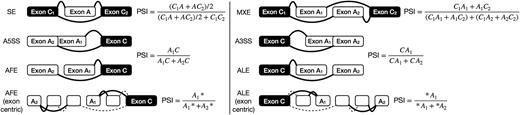
\includegraphics[width=1\textwidth]{images/psichomics/psi-quantification}
  \centering
  \caption[Alternative splicing quantification]{\textbf{Alternative splicing quantification.} Splice junctions required to quantify alternative splicing based on event type. C1A and AC2 represent read counts supporting junctions between a constitutive (C1 or C2, respectively) and an alternative (A) exon and therefore alternative exon A inclusion, while C1C2 represents read counts supporting the junction between the two constitutive exons and therefore alternative exon A exclusion. A1* and A2* represent the sum of read counts supporting junctions spanning the alternative first (A1) and second (A2) exon, respectively. Legend: skipped exon (SE), mutually exclusive exons (MXE), alternative 5$'$ splice site (A5SS), alternative 3$'$ splice site (A3SS), alternative first exon (AFE) and alternative last exon (ALE).}
  \label{fig:psichomics-calc-psi}
\end{figure}

Alternative splicing quantification in psichomics is currently based on exon-exon junction read counts, yet intron retention events require intron-exon junction read counts for their quantification \cite{braunschweig:2014tr}, whereas alternative 5$'$- and 3$'$-UTR require exon body read counts. psichomics does not currently quantify those types of alternative splicing events.

By default, psichomics quantifies all skipped exon events. However, the user can select to measure other types of alternative splicing events (\shortref{fig:psichomics-calc-psi}) and may hand in the list of genes whose alternative splicing events are to be specifically quantified. Furthermore, the step of alternative splicing quantification may be avoided if previously performed. psichomics allows the user to save the quantification of alternative splicing in a file to be loaded in a future session.

\subsection{Data grouping}

psichomics allows to group subjects and their samples or genes and their alternative splicing events for subsequent analysis. Subject and sample grouping can be performed based on available phenotypic (e.g., tissue type and histology) and clinical (e.g., disease stage, smoking history and ethnicity) features. Gene and splicing event grouping relies on respective user-provided identifiers. Moreover, the association between subject/sample groups specified by the user and those defined by the outcome of gene expression and alternative splicing analyses or by other clinical categorical variables can be statistically tested with Fisher's exact tests, implemented with \texttt{stats::fisher.test()}.

\subsection{Dimensionality reduction}
\label{subsec:psichomics-pca}

Dimensionality reduction techniques can be performed on tables containing alternative splicing and gene expression quantifications, with the samples of interest as rows and the selected (if not all) splicing events or genes as columns, after centering and/or scaling the respective distributions (by default, they are only centered).

Principal component analysis (PCA) identifies the combinations of variables that contribute the most to data variance \cite{ringner:2008ve} and it is implemented through the singular value decomposition (SVD) algorithm provided by \texttt{stats::prcomp()}. The total contribution of each variable (splicing event or gene) towards data variance along selected principal components is measured based on \texttt{factoextra::fviz\_contrib()}.

Independent component analysis (ICA), used to decompose data into statistically independent components \cite{hyvarinen:2000vk}, can also be performed based on \texttt{fastICA::fastICA()}, preceded by data centering and/or scaling with \texttt{scale()}.

As many of the aforementioned functions cannot handle missing data, a user-defined threshold for the accepted number of missing values per alternative splicing event or gene (5\%, by default) is used to discard variables before performing dimensionality reduction, whereas the remaining missing values are imputed for each variable as the median from non-missing data samples.

Moreover, samples can be clustered using k-means (based on \texttt{stats::kmeans()}), partitioning around medoids (PAM, \texttt{cluster::pam()}) or clustering large applications (CLARA, \texttt{cluster::clara()}) methods, with the latter being optimised for large datasets and thus the default recommendation.

\subsection{Survival analysis}

Kaplan-Meier estimators (and illustrating curves) \cite{rich:2010wt} and proportional hazard (PH) models \cite{spruance:2004vn} may be applied to groups of patients defined by the user based on clinical features derived, for instance, from TCGA and user-owned data, with survival distributions being compared using the log-rank test. Survival analyses are implemented in psichomics using functions \texttt{Surv()}, \texttt{survfit()}, \texttt{survdiff()} and \texttt{coxph()} from R package \texttt{survival} \cite{therneau:2000tk}.

To evaluate the prognostic value of a given alternative splicing event, survival analysis can be performed on groups of patients separated based on a given alternative splicing quantification (i.e., PSI) cut-off. Patients with multiple samples are assigned the average PSI value of their respective samples after sample filtering (e.g., when using TCGA data, only tumour samples are used for survival analysis by default). When survival differences are estimated for multiple PSI cut-offs for a single alternative splicing event, psichomics suggests the optimal cut-off that minimises the P-value of the log-rank test used to compare survival distributions, graphically supporting the suggestion with a PSI cut-off versus P-value scatter plot. Survival analysis can also be performed on groups defined by an expression cut-off for a selected gene.

\subsection{Differential splicing and gene expression analyses}

In psichomics, analysis of differential splicing between user-defined groups of samples can be performed on all or selected alternative splicing events. Given the non-normal distribution of PSI values \cite{kakaradov:2012wk,jia:2015wy}, median- and variance-based non-parametric tests, such as the Wilcoxon rank-sum (also known as Mann–Whitney U), Kruskal–Wallis rank-sum and Fligner–Killeen tests, are available and recommended \cite{caravela:2015vk}. Levene's and unpaired t-tests can nonetheless be performed as well. All these tests are available through the \texttt{stats} package with their default settings, except for Levene's test that was implemented based on \texttt{car::leveneTest.default()}.

To correct for multiple testing where applicable, P-value adjustment methods for the family-wise error rate (Bonferroni, Holm, Hochberg and Hommel corrections) and the false discovery rate (Benjamini–Hochberg and Benjamini–Yekutieli methods) are available through \texttt{stats::p.adjust()}. By default, multiple testing correction is performed using the Benjamini-Hochberg method.

Although the aforementioned statistical tests are also available to analyse the expression of single genes, genome-wide differential gene expression analysis is implemented based on gene-wise linear model fitting (\texttt{limma::lmFit()} \cite{ritchie:2015tm}) for two selected groups, followed by moderated t-tests and the calculation of log-odds of differential expression, using empirical Bayes moderation of standard errors (\texttt{limma::eBayes()}) and gene-wise variance modelling (\texttt{limma-trend}).

Statistical results can be subsequently explored through density and volcano plots with customisable axes to assist in the identification of the most significant changes when analysing distributions across single or multiple events, respectively. A corresponding table with the results of all statistical analyses is also available and can be retrieved as a tab-delimited plain text file.

\subsection{Correlation between gene expression and PSI values}

The Pearson product-moment correlation coefficient, Spearman's rho (default) and Kendall's tau, all available with \texttt{stats::cor.test()}, can be used to correlate gene expression levels with alternative splicing quantifications. Such analyses allow, for instance, to test the association between the expression levels of RNA-binding proteins (RBPs) and PSI levels of interesting splicing events to identify which of these may undergo RBP-mediated regulation. As such, a list of RBPs is provided in-app \cite{sebestyen:2016tr}, but the user can also define their own group of genes of interest for the test.

\subsection{Feature annotation and literature support}

The representational state transfer (REST) web services provided by Ensembl \cite{yates:2015uo}, UniProt \cite{wu:2006vq}, the Proteins API \cite{nightingale:2017uq} and PubMed \cite{roberts:2001tg} are used in order to annotate genes of interest with relevant biomolecular information (e.g., genomic location, associated transcript isoforms and protein domains, etc.) and related research articles. psichomics also provides the direct link to the cognate entries of relevant external databases, namely Ensembl \cite{cunningham:2015wt}, GeneCards \cite{fishilevich:2016wh}, the Human Protein Atlas \cite{uhlen:2015tg}, the UCSC Genome Browser \cite{goldman:2015un}, UniProt \cite{wu:2006vq} and VAST-DB \cite{tapial:2017ui}.

\subsection{Performance benchmarking}

To measure the time taken by psichomics to load data, normalise gene expression, quantify PSIs for skipped exon events and perform global differential expression and splicing analyses between pairs of GTEx v7 tissues and between normal and primary solid tumour samples from multiple TCGA cohorts (data version 2016\_01\_28 from FireBrowse), the program was run 10 times with the same settings for different combinations of normal human tissues and tumour types in a machine running OS X 10.13.1 with 4 cores and 8GB of RAM, using Safari 11.0.1, RStudio Desktop 1.1.383 and R 3.4.1. The median duration of the 10 runs was used as the performance indicator.

To determine the approximate time complexity of the aforementioned steps in psichomics, gene expression and exon-exon junction quantification datasets were prepared based on approximate distributions obtained from the respective TCGA datasets: negative binomial distributions with a dispersion parameter of 0.25 and 0.2 reads and a mean parameter of 2000 and 100 reads for raw gene expression and exon-exon junction quantification, respectively. Each run was performed on datasets with numbers of samples ranging from 100 to 2500 in intervals of 100 (i.e., 100, 200, 300, …, 2500) and 20 000 genes or 200 000 splice junctions (gene expression or exon-exon junction quantification, respectively). Splice junction identifiers (required for alternative splicing quantification) were randomly retrieved from the TCGA reference annotation. Based on their respective read counts, around 9000 alternative splicing events (i.e., those for which all involved inclusion and exclusion junctions were retrieved) were quantified across selected samples per run. For differential gene expression and splicing analyses, samples were randomly divided into two groups based on the emitted values of a Bernoulli distribution with a probability of success of 50\%.

Polynomials of orders 1–6 were fitted to the relation between running time and the number of samples. As the running time is assumed to always increase with an increasing number of analysed samples, fitted polynomials were constrained to be monotone for 0 or more samples, using \texttt{MonoPoly::monpol()} \cite{murray:2016um}. The best polynomial fits (\shortref{fig:psichomics-performance}) were selected based on analyses of variance (ANOVA) between fitted polynomials of consecutive orders, starting with the comparison between polynomials of orders 1 and 2. A polynomial with higher order is only selected if exhibiting a significantly better fit (p-value $< 0.05$).

\subsection{Alternative splicing quantification benchmarking}

The publicly available RNA-seq data from multiple human, mouse and chicken tissue and cell line samples used in the development of VastDB \cite{tapial:2017ui} were aligned with splice-aware STAR \cite{dobin:2013ts} against the respective transcript-annotated genomes: UCSC hg19 genome assembly and GENCODE v19 annotation for human, UCSC mm10 genome assembly and GENCODE vM14 annotation for mouse, and Ensembl 70 genome assembly and annotation for chicken. In total, 120/706/34 (human/mouse/chicken) exon skipping events quantified by psichomics (function \texttt{psichomics::quantifySplicing()} with default settings) were compared with the respective RT-PCR- and VAST-TOOLS-derived PSI values, available from VastDB \cite{tapial:2017ui}.

Different numbers of junction reads were simulated for different given PSI values to test the impact of read coverage on the accuracy and precision of PSI estimation by psichomics. For each given PSI, junction reads supporting the exon inclusion were simulated as the number of successes obtained from a Bernoulli distribution with the event's junction read coverage (i.e., reads supporting inclusion plus reads supporting exclusion) as the number of observations and the PSI value as the probability of success. Those inclusion reads were then divided by the event's junction read coverage to estimate an ‘observed’ PSI value (as performed by psichomics) that was compared to the given ‘real’ PSI value. These simulations were performed for PSI values from 0 to 1 in 0.1 intervals and event coverages of 10, 20, 50, 100, 500 and 1000 junction read counts, with each combination being tested 10000 times.

TCGASpliceSeq \cite{ryan:2016tm} provides pre-computed alternative splicing quantifications across TCGA cohorts, similarly to \mbox{psichomics}. As such, PSI estimates for each matching (based on genomic coordinates) alternative splicing event and sample from both tools were correlated across the entire TCGA dataset.

\subsection{Continuous integration}
\label{subsec:psichomics-ci}

Continuous integration (CI) tools ensure the automatic testing of software in multiple environments (different versions of operating systems, R, BioConductor, etc.). Currently popular CI tools include Travis CI (macOS and Linux, limited support for Windows), AppVeyor (Windows only) and GitHub Actions (Windows, macOS and Linux). Although psichomics was initially set up with Travis CI and AppVeyor, the flexibility of GitHub Actions in running the three main operating systems and the easiness of adding complex routines led me to replace Travis CI and AppVeyor with GitHub Actions.

psichomics has three GitHub Actions scripts. The first one creates Docker images and stores them in GitHub and Docker Hub for every psichomics release or change in the dev branch. The second one updates the package documentation website via \texttt{roxygen} and \texttt{pkgdown}. The last one builds and checks the R package using \texttt{rcmdcheck::rcmdcheck()} and \texttt{BiocCheck::BiocCheck()} for every change that is committed to the GitHub repository. psichomics is tested in Windows, macOS and Ubuntu, allowing to automatically check if the package builds correctly and if it passes all unit tests (created using testthat) in multiple platforms, among other checks. The code coverage of the package is then tested via Codecov. All of these tools are free for open-source projects.

\section{Results}

psichomics' web app is available at \alink{compbio.imm.medicina.ulisboa.pt/psichomics}. Alternatively, users can install psichomics in their own computers, allowing them to use local computing resources. psichomics offers both a graphical and a command-line interface. Although most features are common to both interfaces, we recommend less experienced users to opt for the Shiny-based graphical interface. To start the graphical interface in the local version, load the psichomics package in R via \texttt{library(psichomics)} and run \texttt{psichomics()}. The user's default web browser will be launched with a local version of the psichomics web app.

\subsection{Case study}

Several splicing factors have been reported to be involved in pluripotency, including SRSF3, MBNL1/2, RBFOX2, and U2AF1 \cite{zavolan:2018vi,han:2013ww,venables:2013tz,chen:2015wm}. For instance, MBNL1/2 regulates the mutually exclusive inclusion of two \emph{FOXP1} exons, inducing a switch from its pluripotency-associated FOXP1-ES protein isoform, that promotes the expression of \emph{OCT4}, \emph{NANOG}, and other key pluripotency transcription factors, to the canonical differentiation-inducing FOXP1 isoform \cite{gabut:2011wk}.

The early stage of somatic cell reprogramming, characterised by acquisition of pluripotency features, is related with mesenchymal-to-epithelial transition, a crucial development-related process affecting cell polarity and adhesion that is mediated by the aforementioned splicing regulators \cite{zavolan:2018vi,pradella:2017wp}. Consistently, the alternative splicing modulation of epithelial-to-mesenchymal transition is linked with both cancer progression and metastasisation and with the generation of cancer stem cells, characterised by enhanced self-renewal, proliferation, and other stemness properties \cite{zavolan:2018vi,pradella:2017wp,aponte:2017wv}.

% We will analyse genetically (i.e., isogenic) and not genetically (nonisogenic) matched human fibroblast and (embryonic and induced-pluripotent) stem cell RNA-seq samples \cite{choi:2015tu}, together with GTEx and TCGA data, using psichomics to highlight putative differentially spliced events between such conditions and candidate RNA-binding protein regulators of those events.

% We will automatically retrieve preprocessed data for the chosen dataset from recount2. We will conduct a typical workflow of filtering and normalising gene expression and quantifying and filtering AS, followed by statistical analyses to identify differentially expressed genes and spliced events between isogenic human fibroblasts and stem cells. We will then correlate the expression of genes encoding for RNA-binding proteins with the PSI values of the most interesting AS events, in the stem cell dataset as well as across multiple tissues (GTEx data) and cancer types (TCGA data), to identify among the former putative regulators of the latter. Finally, the pan-cancer prognostic value of a select AS event will be assessed.

% We hereby show an example of an integrative workflow (both in terms of methods and datasets used) that can be performed using psichomics.

Using the graphical interface of psichomics, we analysed SRA project SRP063867 \cite{choi:2015tu} containing genetically (i.e., isogenic) and not genetically (nonisogenic) matched human induced-pluripotent stem cells (iPSC), embryonic stem cells (ESC), and fibroblasts to compare changes in alternative splicing between isogenic stem cells and isogenic fibroblasts. The code to run this analysis is publicly available at \alink{github.com/nuno-agostinho/stem-cell-analysis-in-psichomics}.

\subsubsection{Data loading}

We used psichomics to download preprocessed RNA-seq data for SRP063867 via recount2 \cite{collado-torres:2017uw}, including sample annotation, raw gene expression and exon–exon junction read counts. psichomics automatically downloads the data, loads the workspace and displays information per dataset (\shortref{fig:psichomics-gene-expr-summary}).

\begin{figure}[!ht]
  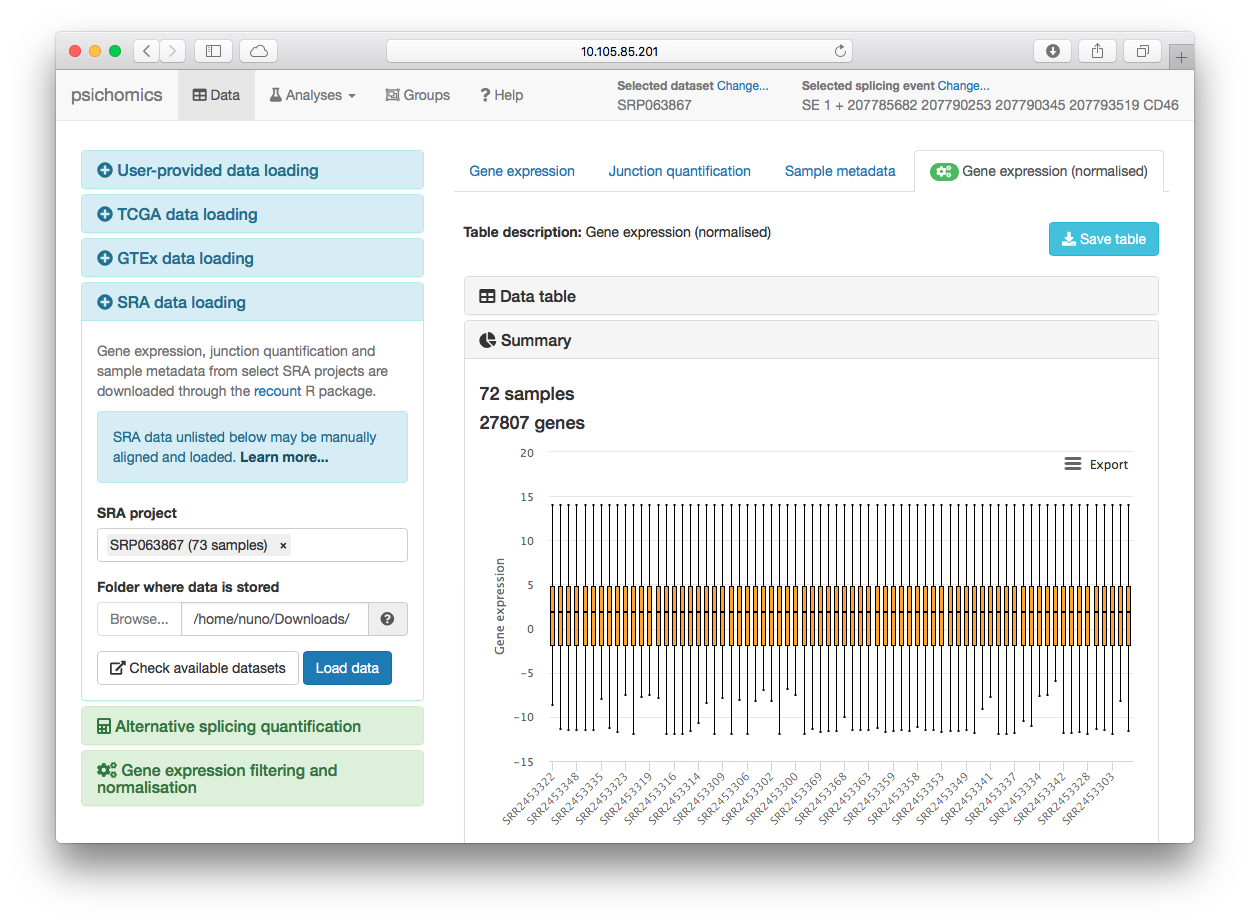
\includegraphics[width=\textwidth]{images/psichomics/0-gene-expr-summary}
  \centering
  \caption[Summary information on datasets]{\textbf{Summary information on datasets.} psichomics presents information on the loaded datasets in a dedicated tab. That information includes summary statistics, like the numbers of samples and genes profiled in each dataset, and plots, like the shown boxplot to visualise the distribution of normalised gene read counts per sample.}
  \label{fig:psichomics-gene-expr-summary}
\end{figure}

\subsubsection{Gene expression filtering and normalisation}

Next, we performed gene expression filtering and normalisation on the loaded raw gene expression read counts using psichomics default settings (based on the \texttt{edgeR} \cite{robinson:2010wx} and \texttt{limma} \cite{ritchie:2015tm} R packages). We filtered out lowly-expressed genes with a minimum of 10 read counts for at least one sample and with a minimum total read counts of 15 (default settings in psichomics). We noticed that the density plot of the samples’ library size (i.e., the total number of mapped reads) suggests relatively low read coverage for sample SRR2453313 (\shortref[a]{fig:psichomics-ge-norm}). At this time, we decided to keep this sample to compare with other samples after data normalisation.

Afterwards, we normalised gene expression values by scaling raw library sizes across samples. Default gene expression normalisation scales for raw library sizes based on weighted trimmed mean of M-values (TMM) \cite{robinson:2010wx}, followed by computation of log2-transformed counts per million values. The default normalisation is not fully effective, as very different distributions between samples are observed (\shortref[b]{fig:psichomics-ge-norm}).

\begin{figure}[!ht]
  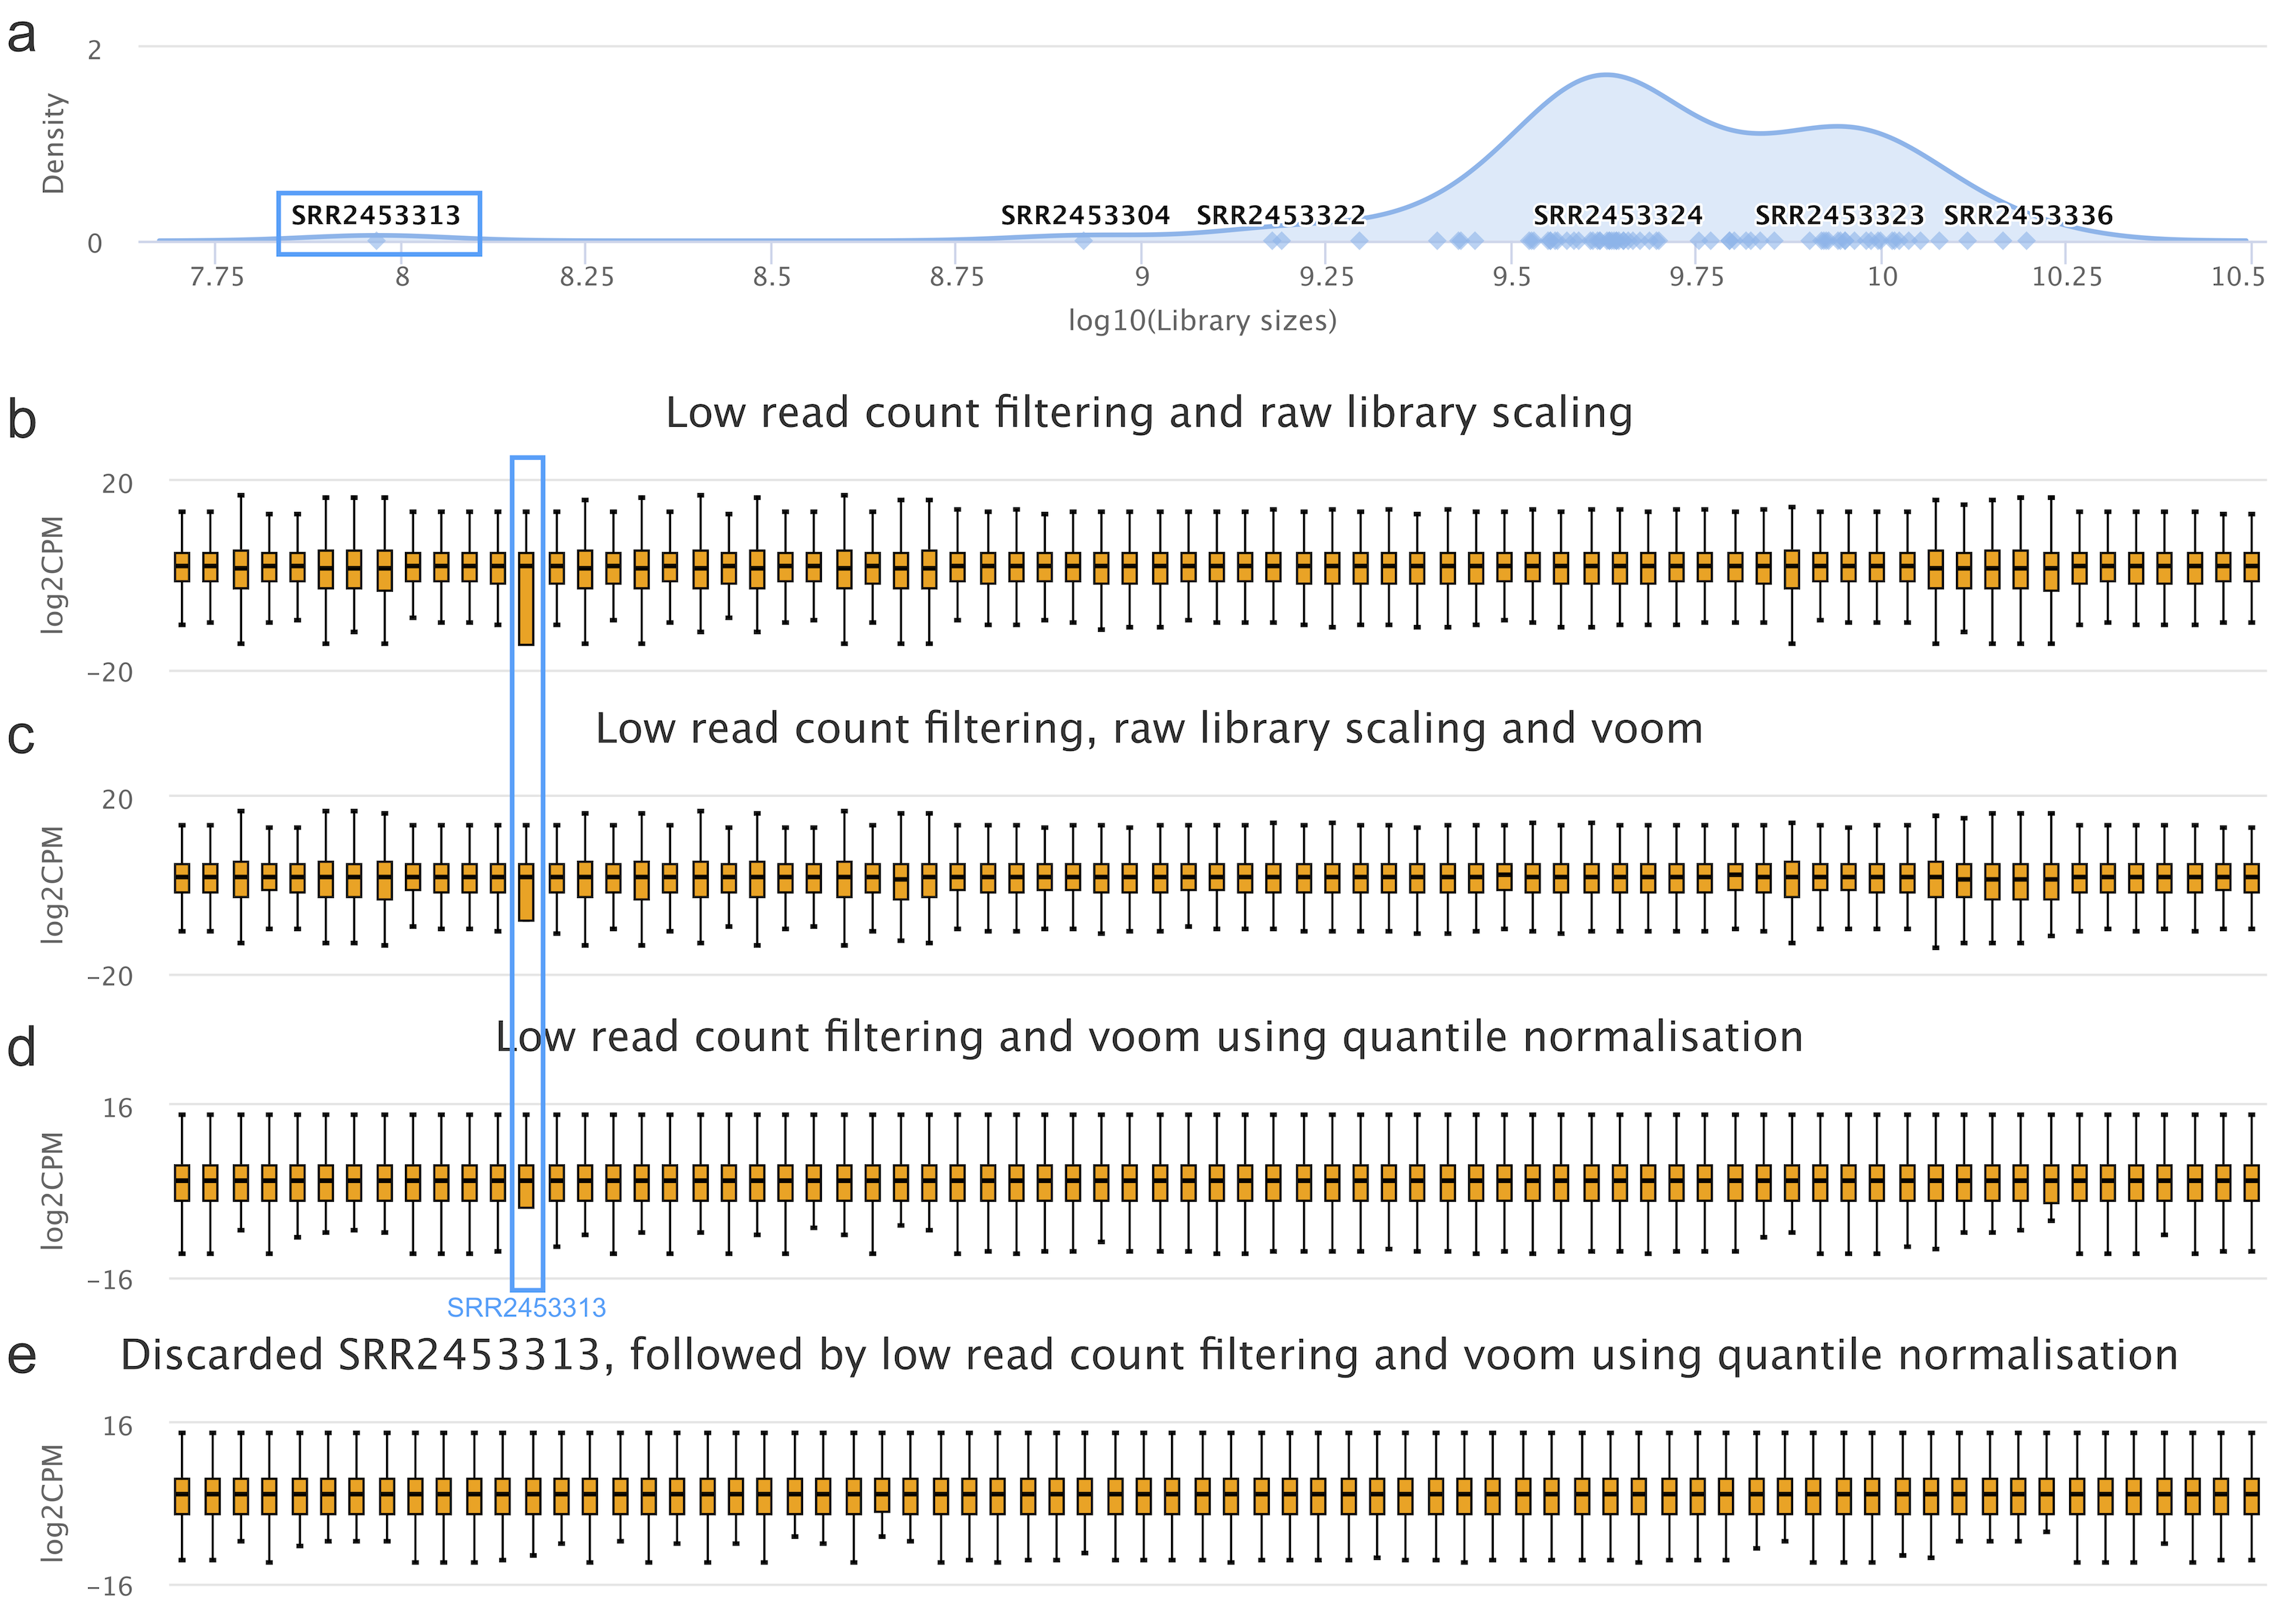
\includegraphics[width=1\textwidth]{images/psichomics/1-gene-expr-normalisation}
  \centering
  \caption[Gene expression normalisation]{\textbf{Gene expression normalisation.} (a) Density plot of the distribution of raw library sizes (i.e., total number of mapped read counts) across samples. Highlighted with the blue label is the sample with the smallest library. (b–e) Boxplots of distribution of gene expression in log2-transformed counts per million (log2CPM per sample after low read count filtering and raw library scaling (b), this procedure followed by voom modeling (c), voom modeling using quantile normalisation instead of raw library scaling (d), and the latter after discarding the sample with the smallest library, highlighted in blue (e).}
  \label{fig:psichomics-ge-norm}
\end{figure}

We used voom instead, as it incorporates the mean-variance relationship of the data to normalise expression levels between samples \cite{ritchie:2015tm}. The distributions remain heterogeneous (\shortref[c]{fig:psichomics-ge-norm}) based on the default weighted trimmed mean of M-values (TMM) \cite{robinson:2010wx}, used to normalise for library sizes, so we replaced it by quantile normalisation \cite{ritchie:2015tm}. This more vigorous normalisation of gene read counts made their distributions comparable across samples, except for SRR2453313 (\shortref[d]{fig:psichomics-ge-norm}) that was thus discarded. No obvious outlying gene expression distribution is apparent after discarding that sample and renormalising (\shortref[e]{fig:psichomics-ge-norm}). The filtered and normalised gene expression dataset was now composed of 72 samples and 27 807 genes.

\subsubsection{Alternative splicing quantification}

The percent spliced-in (PSI) metric is commonly employed to measure the relative abundance of the inclusion isoform of an alternative splicing event \cite{wang:2008wa}. For each annotated event, psichomics was used to quantify PSI values based on the ratio of splice (exon–exon) junction read counts that support the inclusion of the alternative sequence. The selected alternative splicing annotation was \emph{Human hg38 (2018-04-30)}.

The default event types were quantified: skipped exon (SE), mutually exclusive exon (MXE), alternative first and last exon (AFE and ALE, respectively), and alternative 3$'$ and 5$'$ splice site (A3SS and A5SS, respectively). By default, only alternative splicing events with a minimum of 10 junction read counts supporting either inclusion or exclusion of the alternative sequence are considered to avoid quantifying events with insufficient evidence. For consistency with gene expression analysis, we discarded sample SRR2453313 with the lowest library size.

\begin{wrapfigure}{r}{.7\textwidth}
  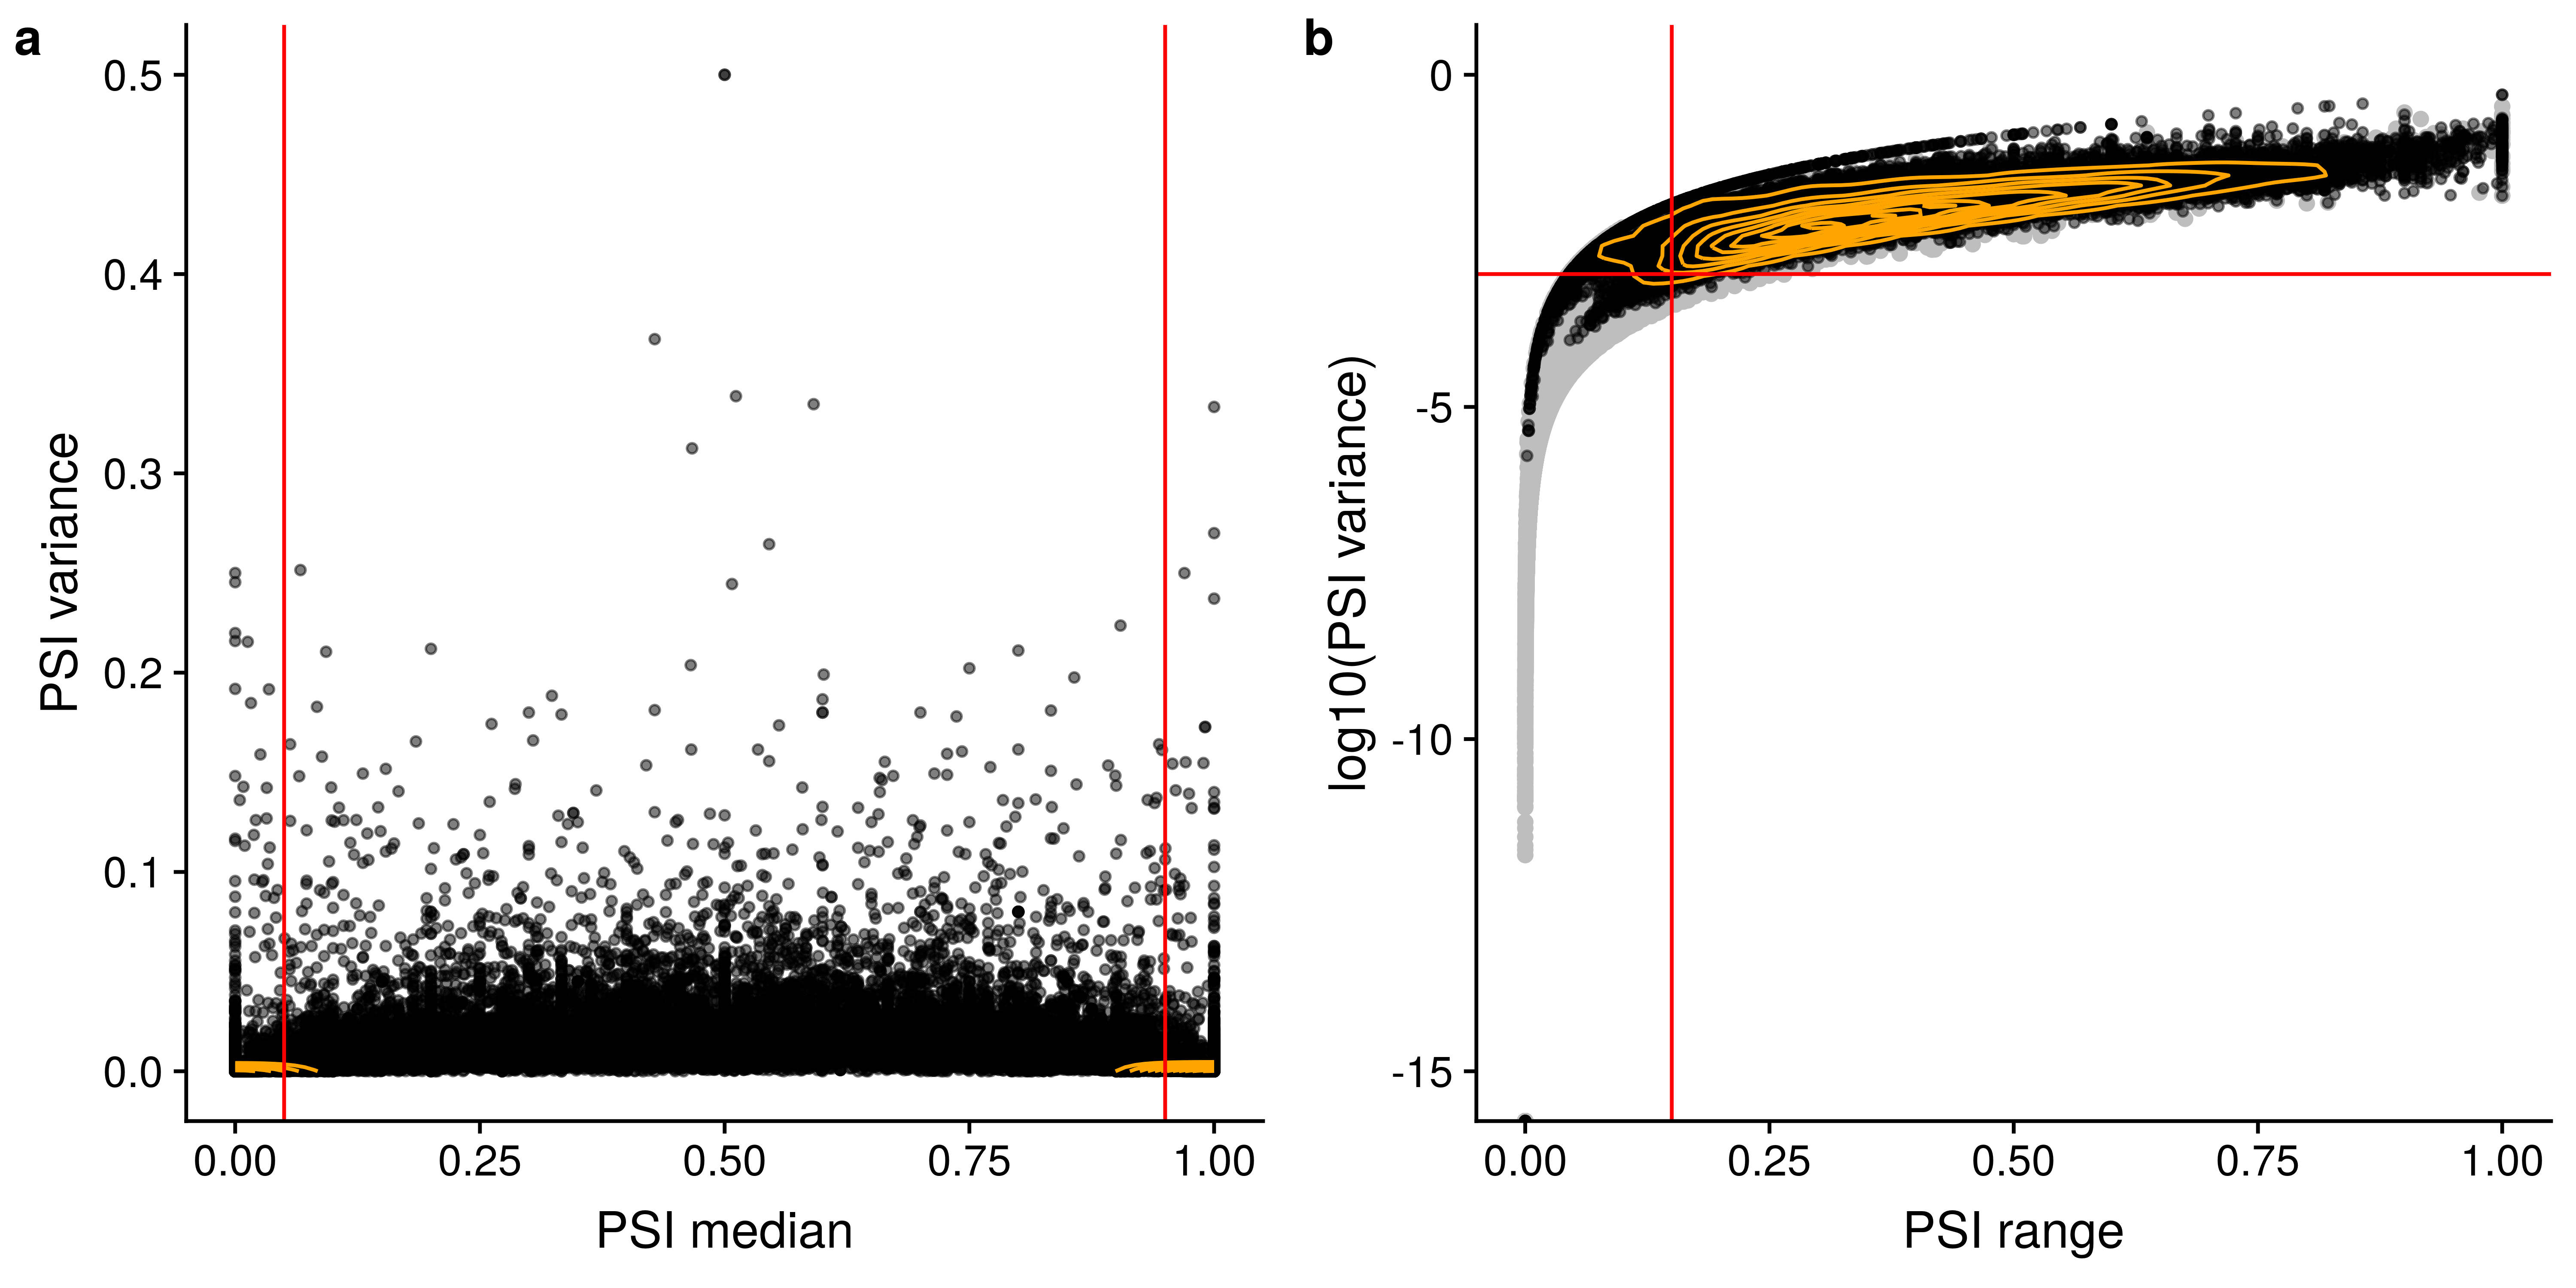
\includegraphics[width=\linewidth]{images/psichomics/4-psi-filtering}
  \caption[Alternative splicing quantification filtering]{\textbf{Alternative splicing quantification filtering.} (a) Selection, for further analyses, of alternative splicing events with median PSI values between 0.05 and 0.95. (b) Further filtering those events with $\textrm{PSI range} > 0.15$ and $log_{10}(\textrm{variance}) > -3$. For illustration purposes, grey points represent the events discarded in panel a.}
  \label{fig:psichomics-psi-filtering}
\end{wrapfigure}

In total, a high number of 135 717 alternative splicing events were quantified. However, only events exhibiting some variance across samples are informative when analysing differential splicing. We therefore filtered out low-variance events with median PSI values between 0.05 and 0.95 (\shortref[a]{fig:psichomics-psi-filtering}), avoiding those whose median PSI is consistently near 0 and 1 (i.e., splicing events that are mostly constitutive). This concomitantly filters out events of very low variance (\shortref[b]{fig:psichomics-psi-filtering}). To further select events that vary across samples based on a minimum PSI variance, we set $log_{10}(variance) > -3$ (\shortref[b]{fig:psichomics-psi-filtering}). Alternative splicing events were further filtered based on their PSI range (maximum — minimum PSI value across samples), as a surrogate for the minimum changes in alternative splicing that can be considered biologically meaningful, by setting the minimum PSI range to 0.15 (\shortref[b]{fig:psichomics-psi-filtering}). The number of potentially interesting events was reduced from 135 717 to 27 401.

%\begin{figure}[!ht]
%  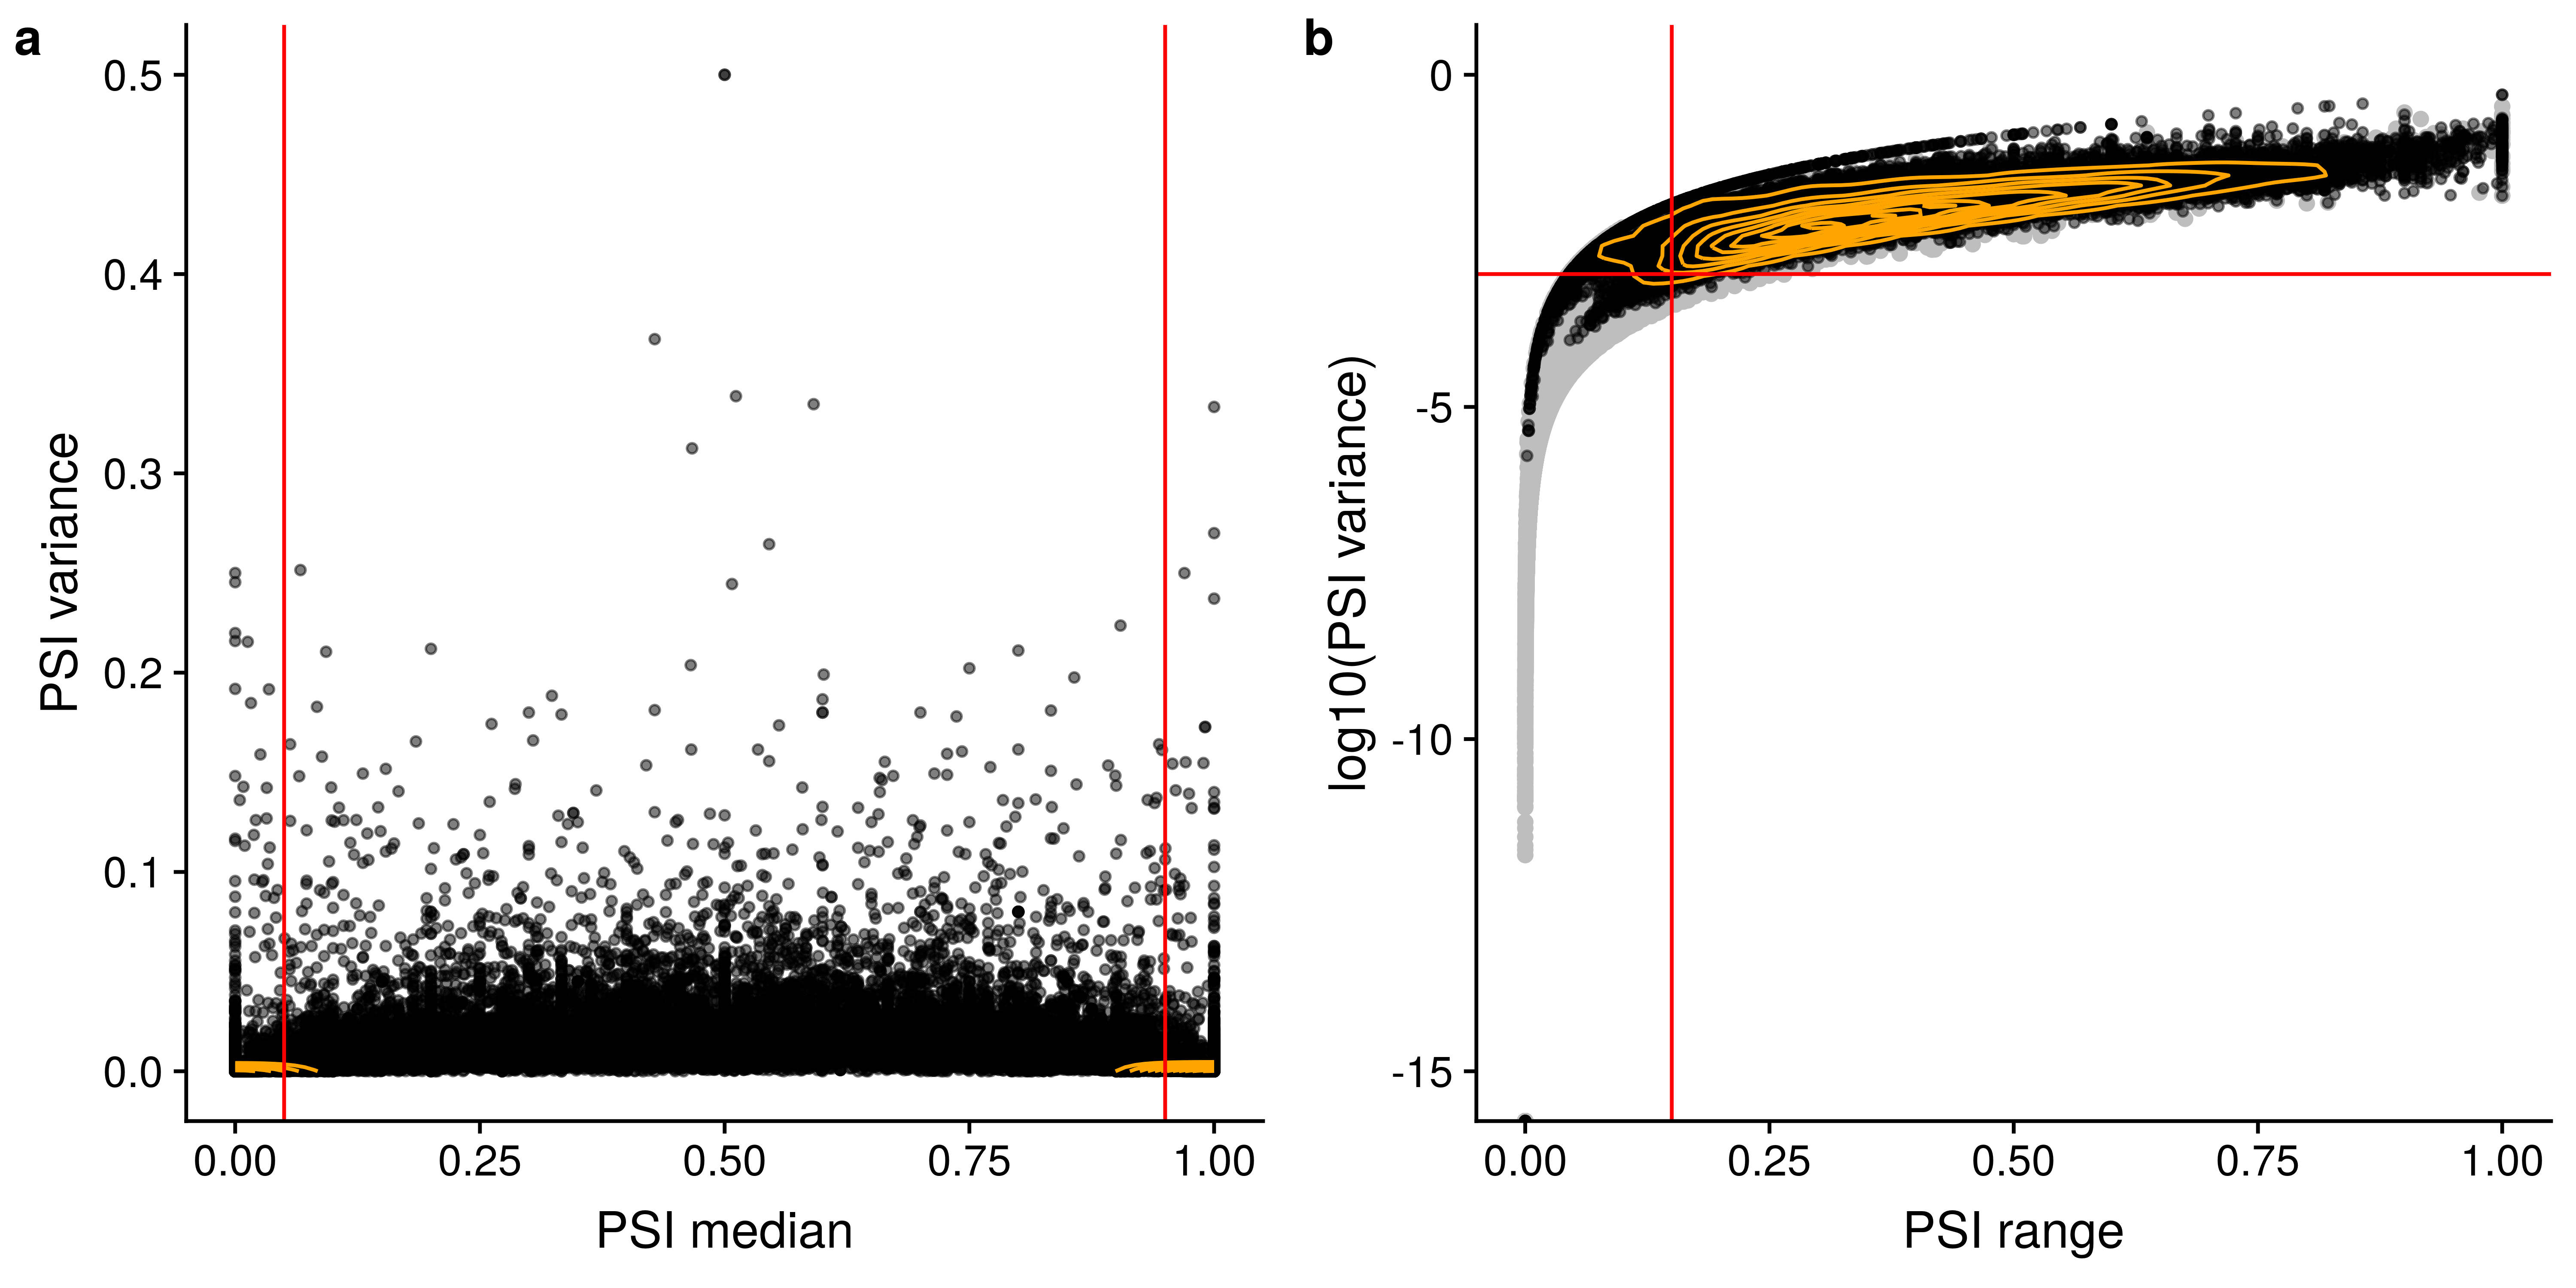
\includegraphics[width=.7\textwidth]{images/psichomics/4-psi-filtering}
%  \centering
%  \caption[Alternative splicing quantification filtering]{\textbf{Alternative splicing quantification filtering.} (a) Selection, for further analyses, of alternative splicing events with median PSI values between 0.05 and 0.95. (b) Further filtering those events with $\textrm{PSI range} > 0.15$ and $log_{10}(\textrm{variance}) > -3$. For illustration purposes, grey points represent the events discarded in panel a.}
%  \label{fig:psichomics-psi-filtering}
%\end{figure}

\subsubsection{Principal component analysis (PCA)}

Data groups can be created in psichomics based on sample/subject matched metadata or on alternative splicing events and respective genes. We grouped ESC and iPSC samples together to compare them against Isogenic Stem Cells and Isogenic Fibroblasts.

%\begin{figure}
%      \centering
%      \begin{subcaptiongroup}
%      	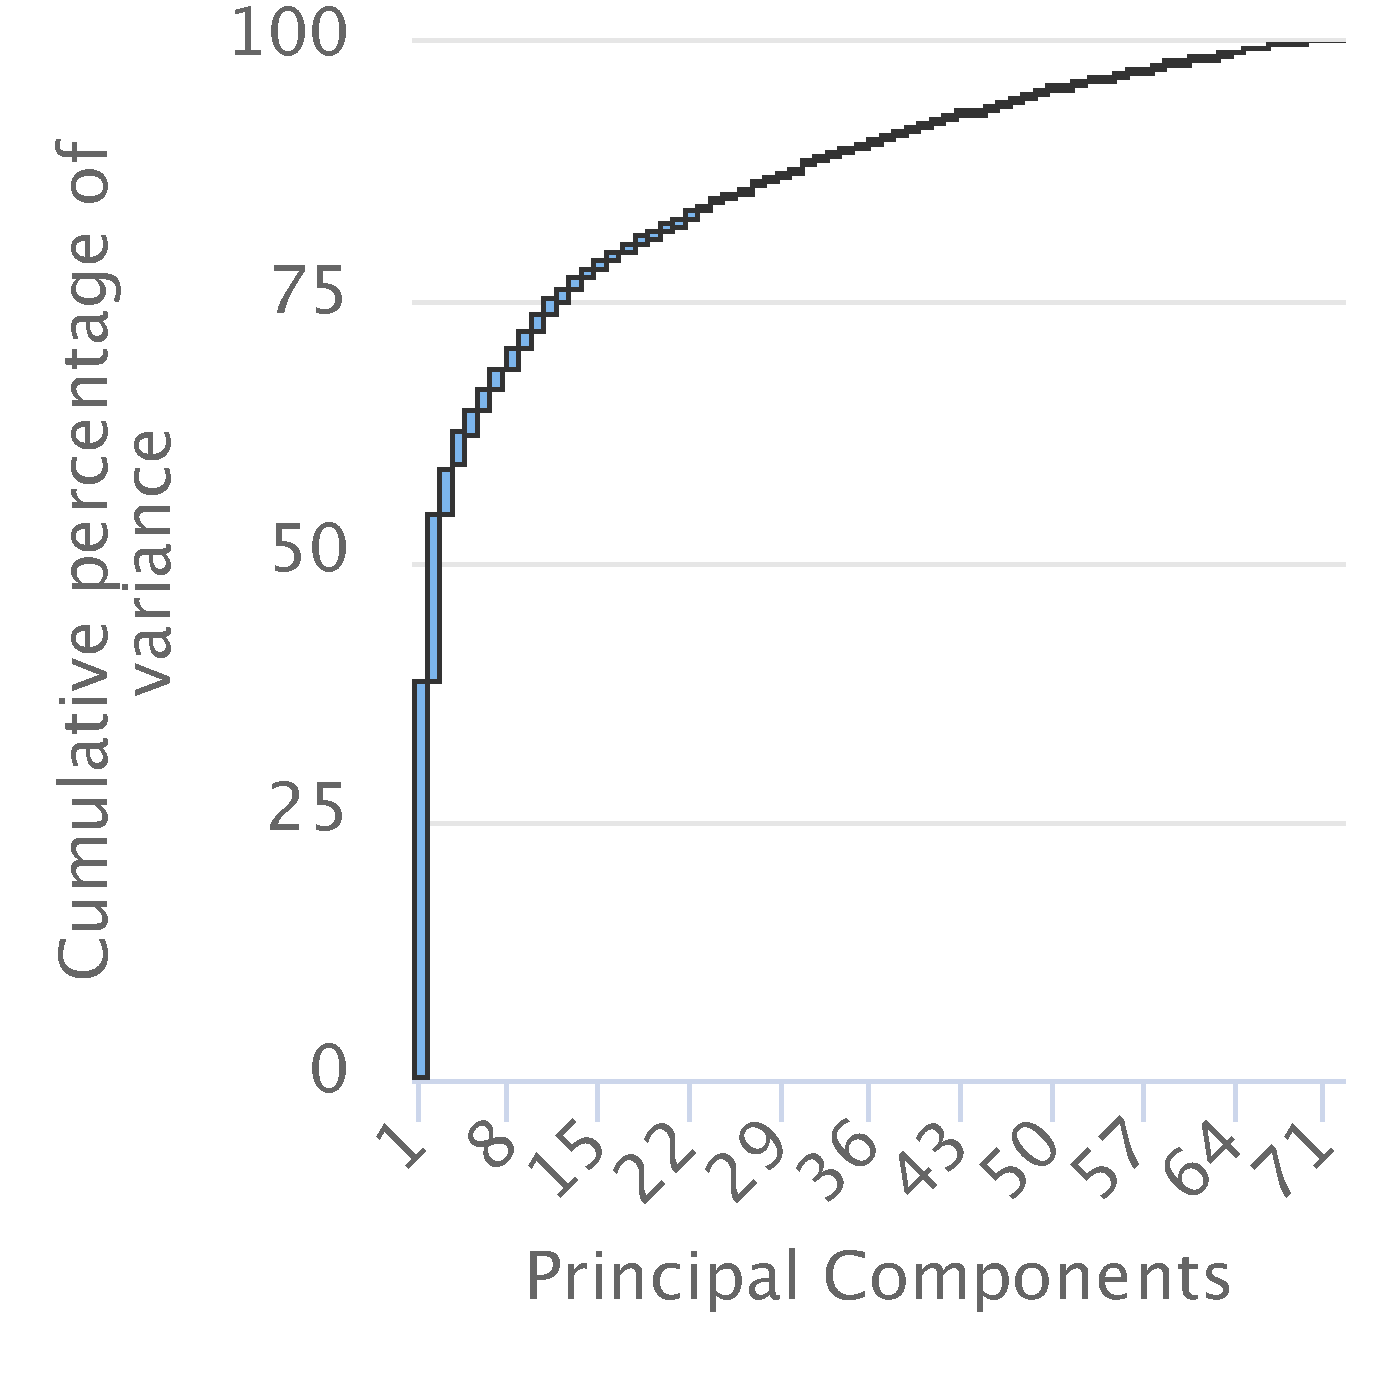
\includegraphics[width=0.2\textwidth]{images/psichomics/5-pca/a}
%      	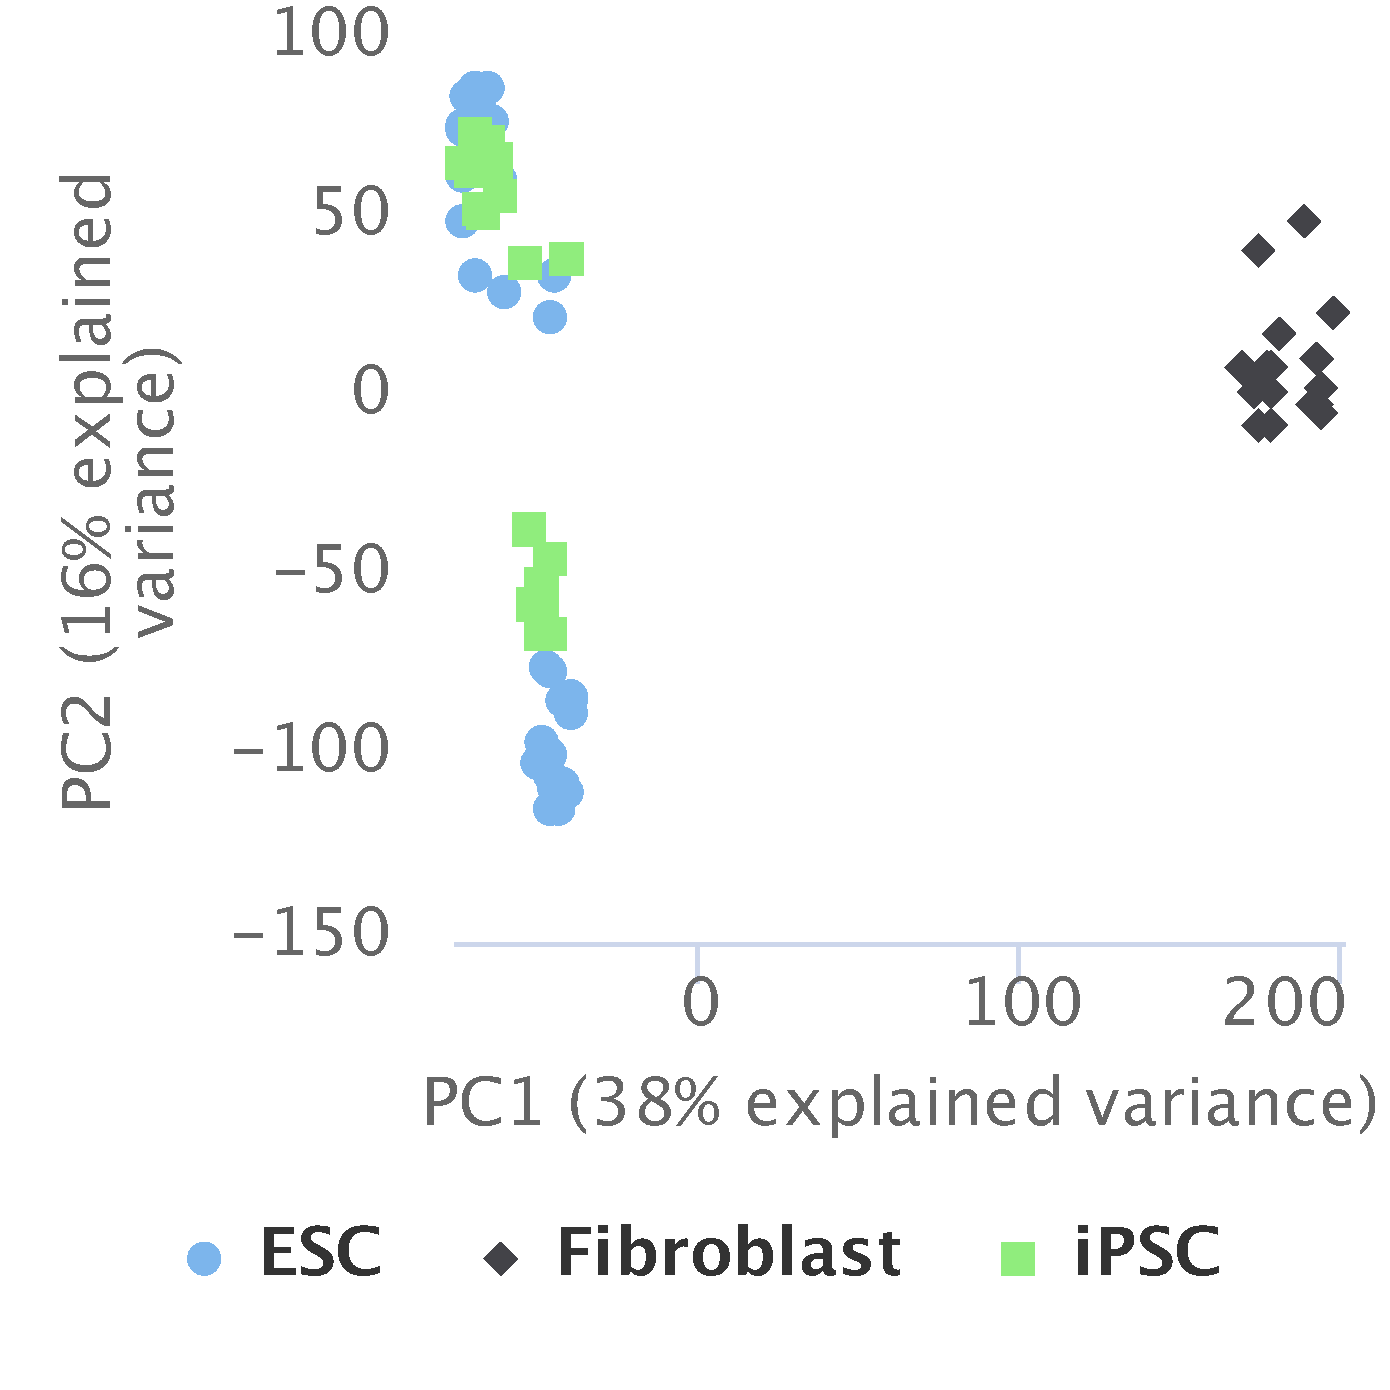
\includegraphics[width=0.2\textwidth]{images/psichomics/5-pca/b}
%      \end{subcaptionblock}
%      \caption{Two animals}\label{animals}
%\end{figure}

\begin{figure}[!ht]
	\centering
	\begin{subfigure}[h]{0.32\textwidth}
		\begin{overpic}[abs,width=\textwidth]{images/psichomics/5-pca/a}
			\put(6,137){\textsf{\textbf{a}}}
		\end{overpic}
	\end{subfigure}
	\begin{subfigure}[h]{0.32\textwidth}
		\begin{overpic}[abs,width=\textwidth]{images/psichomics/5-pca/b}
			\put(6,137){\textsf{\textbf{b}}}
		\end{overpic}
	\end{subfigure}
	\begin{subfigure}[h]{0.32\textwidth}
		\begin{overpic}[abs,width=\textwidth]{images/psichomics/5-pca/c}
			\put(6,137){\textsf{\textbf{c}}}
		\end{overpic}
	\end{subfigure}
	\begin{subfigure}[h]{0.32\textwidth}
		\begin{overpic}[abs,width=\textwidth]{images/psichomics/5-pca/d}
			\put(6,137){\textsf{\textbf{d}}}
		\end{overpic}
	\end{subfigure}
	\begin{subfigure}[h]{0.32\textwidth}
		\begin{overpic}[abs,width=\textwidth]{images/psichomics/5-pca/e}
			\put(6,137){\textsf{\textbf{e}}}
		\end{overpic}
	\end{subfigure}
	\begin{subfigure}[h]{0.32\textwidth}
		\begin{overpic}[abs,width=\textwidth]{images/psichomics/5-pca/f}
			\put(6,137){\textsf{\textbf{f}}}
		\end{overpic}
	\end{subfigure}
	\begin{subfigure}[h]{0.96\textwidth}
		\begin{overpic}[abs,width=\textwidth]{images/psichomics/5-pca/g}
			\put(-10,70){\textsf{\textbf{g}}}
		\end{overpic}
	\end{subfigure}
    \caption[Principal component analysis]{\textbf{PCA of normalised gene expression (a–d) and alternative splicing quantification data (e–g).} (a) Plot displaying the cumulative percentage of total gene expression data variance explained by each principal component. (b, d) Scatter plots of scores of each sample on principal components 1 and 2, with samples coloured based on cell type (b) and isogenicity (d). (c) Scatter plot of loadings of each gene on principal components 1 and 2. Each gene’s bubble size is proportional to its relative contribution to principal components 1 and 2. For performance reasons, only the 100 most contributing variables (i.e., genes or alternative splicing events) to the selected principal components are plotted by default. (e, f) Scatter plots of scores of each sample on principal components 1 and 2, with samples coloured based on cell type (e) and isogenicity (f). (g) Table of loadings of the 5 alternative splicing events contributing the most to principal components 1 and 2.}
    \label{fig:psichomics-pca}
\end{figure}

%\begin{figure}[!p]
%  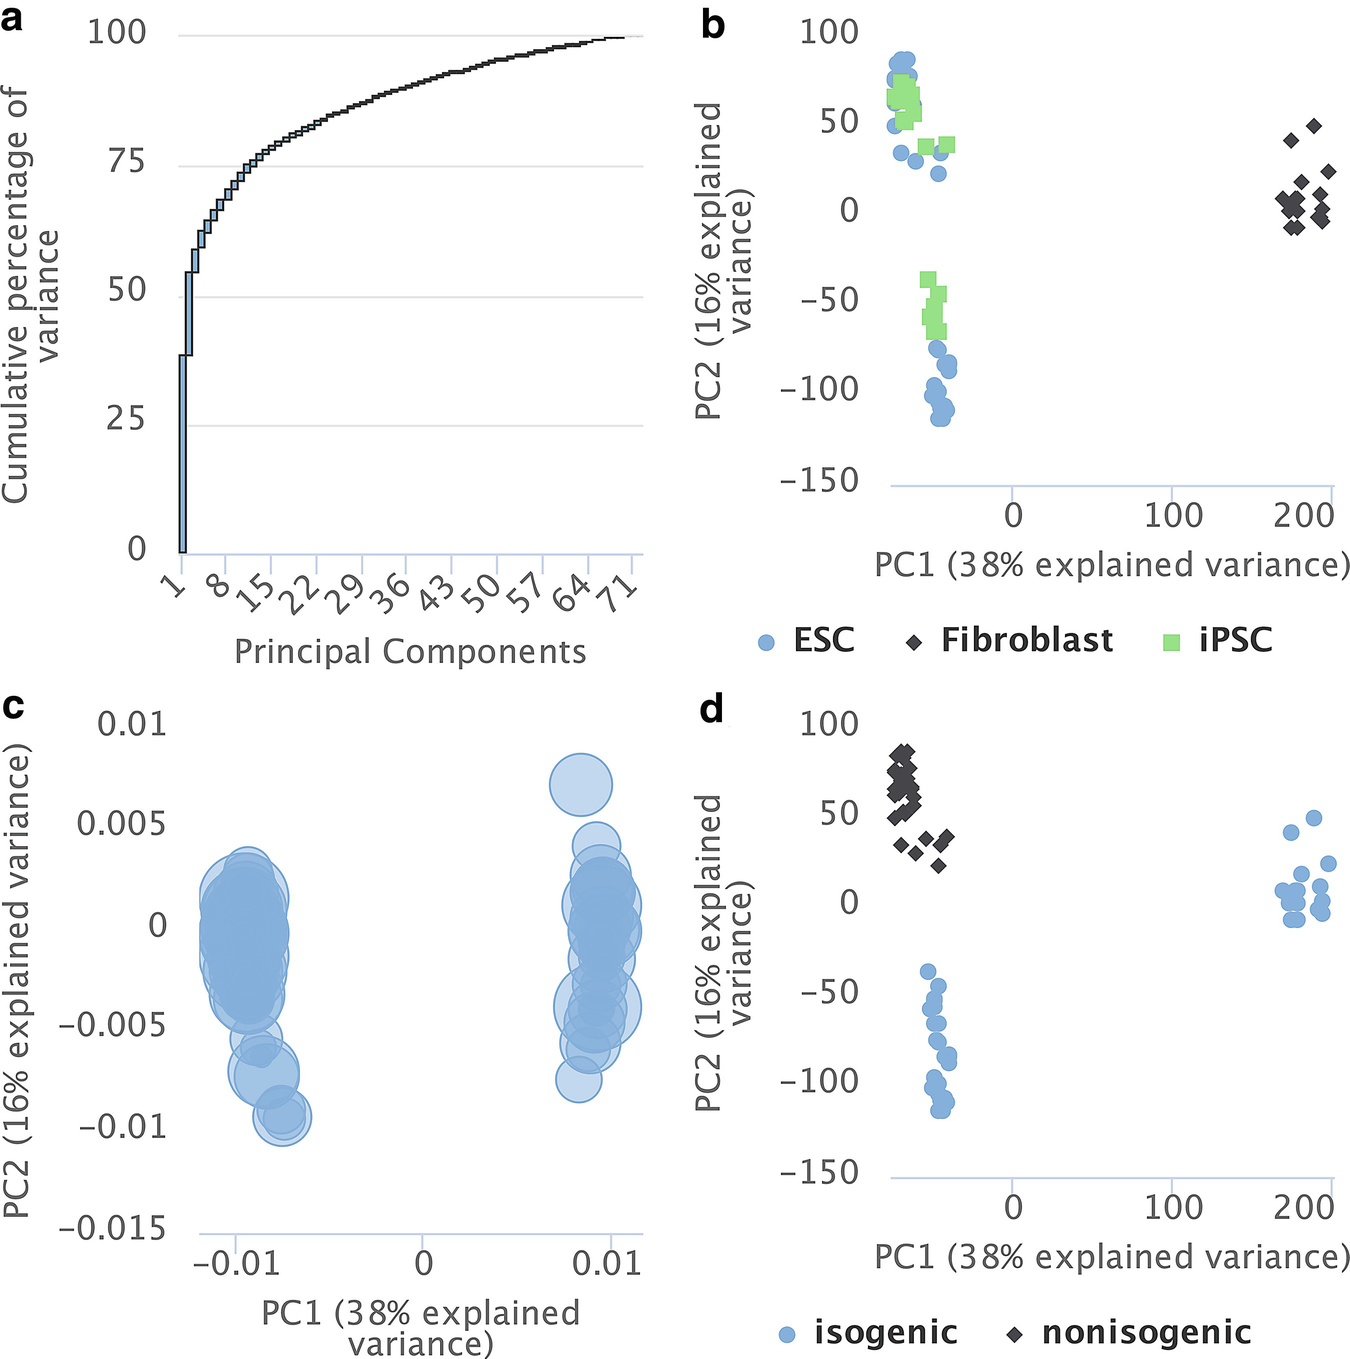
\includegraphics[width=.7\textwidth]{images/psichomics/5-pca-a}
%  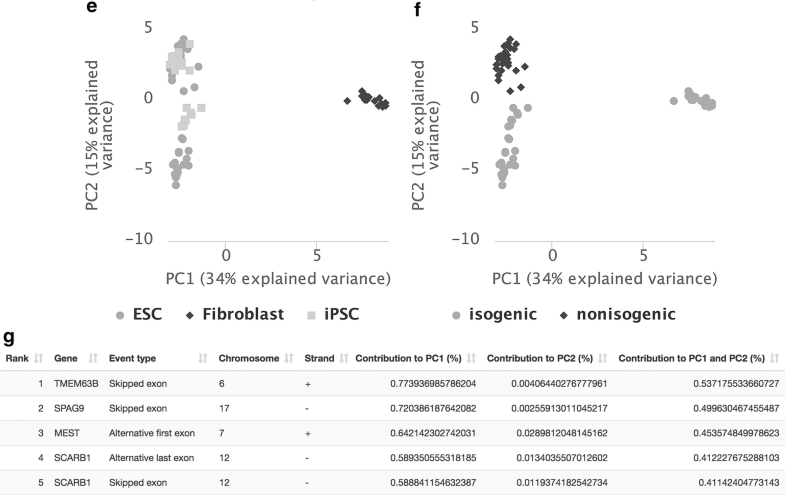
\includegraphics[width=.9\textwidth]{images/psichomics/5-pca-b}
%  \centering
%\end{figure}

Later we performed PCA on normalised gene expression after centring and scaling the values. We allowed to impute at most 4 (i.e., around 5\% of the 72 samples) tolerated missing values per row\footnote{More information in \fullref{subsec:psichomics-pca}.}. The first two principal components explain around 50\% of the observed variance in the data.

The variance observed across principal component 1 seems to be related with the cell type (fibroblast versus stem cell) (\shortref[b]{fig:psichomics-pca}), whereas principal component 2 is associated with isogenicity (i.e., isogenic vs nonisogenic; respective column named dataset type in the SRA metadata) (\shortref[d]{fig:psichomics-pca}). From the 15 most variance-contributing genes, as displayed in the table below the loading plot, at least \emph{DNMT3B} and \emph{RBPMS2} have been previously associated with pluripotency \cite{fagoonee:2013vx}. Specifically, \emph{RBPMS2} has been reported to play a role in self-renewal following the knockdown of \emph{ESRP1}, reported to act as a regulator of pluripotency \cite{fagoonee:2013vx}.

Similarly, we performed and plotted PCA on alternative splicing data\footnote{PSI values are not scaled by default, given they are dimensionless ratios that range from 0 to 1.}. Akin to the observations from PCA plots on normalised gene expression, principal component 1 appear to be associated with cell type and principal component 2 with isogenicity (\shortref[e-f]{fig:psichomics-pca}). The table below the loading plot allows to assess which alternative splicing events contribute the most to those separations (\shortref[g]{fig:psichomics-pca}). Some of the cognate genes of those events have already been reported to be involved in conserved splicing programs in stem cell differentiation, including \emph{KIF13A} and \emph{PALM} \cite{venables:2013tz}.

\subsubsection{Differential expression and splicing analysis}

We performed differential gene expression and differential splicing analysis between isogenic stem cells and isogenic fibroblasts (\shortref{fig:psichomics-diff-analyses}). First, normalised gene expression was linearly modelled, with explanatory variables defined based on the selected groups. Moderated t-tests and log-odds of differential expression were then computed by empirical Bayes moderation of the standard errors towards a common value \cite{ritchie:2015tm}.

\begin{figure}[!ht]
  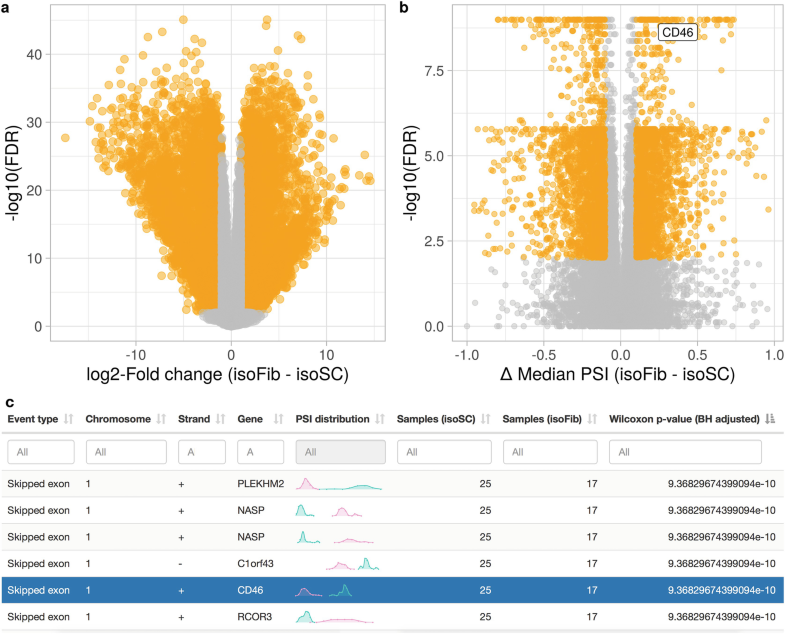
\includegraphics[width=.7\textwidth]{images/psichomics/6-diff-analyses}
  \centering
  \caption[Differential expression and splicing analyses]{\textbf{Differential expression (a) and splicing (b, c) analyses.} (a, b) Volcano plots where orange-highlighted genes/events correspond to $\textrm{adjusted p-value} < 0.01$ and either $|log_2(\textrm{Fold change})| > 1$ (a) or $|\Delta \textrm{ median PSI}| > 0.1$ (b). The \emph{CD46} penultimate exon inclusion is labeled in b with the cognate gene symbol. (c) Table showing a subset of the differential splicing results, sorted in ascending order by the adjusted p-value of Wilcoxon’s rank-sum test. PSI distributions are colored by groups: pink for isogenic stem cells (isoSC) and green for isogenic fibroblasts (isoFib). The selected alternative splicing event (in blue) depicts the \emph{CD46} penultimate exon inclusion.}
  \label{fig:psichomics-diff-analyses}
\end{figure}

%\begin{figure}[!ht]
%  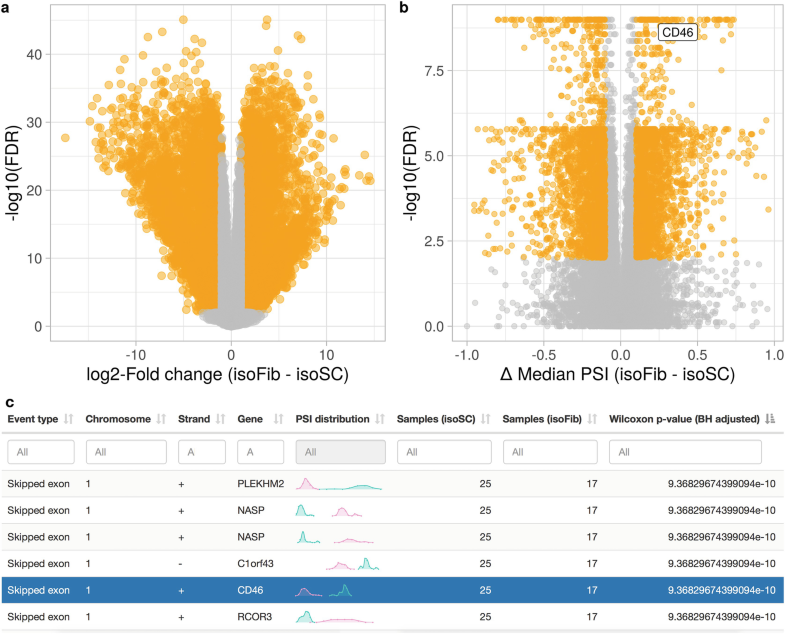
\includegraphics[width=.7\textwidth]{images/psichomics/6-diff-analyses}
%  \centering
%  \caption[Differential expression and splicing analyses]{\textbf{Differential expression (a) and splicing (b, c) analyses.} (a, b) Volcano plots where orange-highlighted genes/events correspond to $\textrm{adjusted p-value} < 0.01$ and either $|log_2(\textrm{Fold change})| > 1$ (a) or $|\Delta \textrm{ median PSI}| > 0.1$ (b). The \emph{CD46} penultimate exon inclusion is labeled in b with the cognate gene symbol. (c) Table showing a subset of the differential splicing results, sorted in ascending order by the adjusted p-value of Wilcoxon’s rank-sum test. PSI distributions are colored by groups: pink for isogenic stem cells (isoSC) and green for isogenic fibroblasts (isoFib). The selected alternative splicing event (in blue) depicts the \emph{CD46} penultimate exon inclusion.}
%  \label{fig:psichomics-diff-analyses}
%\end{figure}

The volcano plot of differential splicing analysis between isogenic stem cells and fibroblasts (\shortref[b]{fig:psichomics-diff-analyses}) exhibits two strata, that is, two modes of Wilcoxon’s test significance. The significance stratum in the top is the result of using such nonparametric test (motivated by the non-normality of PSI distributions) when all values in one of the groups are higher than those in the other group; the number of tested groups also affects the significance of the difference. The lower significance stratum relates to a consistent number of repeated values between samples (usually occurring when one of the groups is closer to a PSI value of 0 or 1). As the Wilcoxon’s test is rank-based, some ranks are not unique if there are two identical values; this occurrence (called a tie) hampers the computation of exact p-values. Increasing the number of identical values when performing the Wilcoxon’s test decreases the significance of the comparison, which may bias the significance of differentially spliced events when one of the groups is characterised by PSI values close to 0 or 1 (constitutive splicing) and will therefore present many 0's or many 1's.

\subsubsection{Skipping of \emph{CD46} penultimate exon}

The skipping of the penultimate exon of \emph{CD46} is one of the most significantly differentially spliced sequences between isogenic fibroblasts and isogenic stem cells in our analyses (\shortref[b-c]{fig:psichomics-diff-analyses}). Based on its PSI distributions in the different cell types, higher inclusion of the \emph{CD46} penultimate exon is associated with fibroblasts, whereas lower inclusion is associated with stem cells, both ESC and iPSC (\shortref[a]{fig:psichomics-cd46-as}). The inclusion of \emph{CD46} penultimate exon leads to a premature termination codon that may cause the respective transcript to be targeted for nonsense-mediated decay \cite{warzecha:2010wi}.

\begin{figure}[!p]
	\centering
	\begin{subfigure}[h]{0.8\textwidth}
		\begin{overpic}[abs,width=\textwidth]{images/psichomics/7-cd46-as/a}
			\put(2,225){\textsf{\textbf{a}}}
		\end{overpic}
	\end{subfigure}
	\begin{subfigure}[h]{0.8\textwidth}
		\begin{overpic}[abs,width=\textwidth]{images/psichomics/7-cd46-as/b-c}
			\put(2,165){\colorbox{white}{\textsf{\textbf{b}}}}
			\put(176,165){\colorbox{white}{\textsf{\textbf{c}}}}
		\end{overpic}
	\end{subfigure}
	\begin{subfigure}[h]{0.8\textwidth}
		\begin{overpic}[abs,width=\textwidth]{images/psichomics/7-cd46-as/d}
			\put(2,157){\textsf{\textbf{d}}}
		\end{overpic}
	\end{subfigure}
    \label{fig:eif4g1-compound-plots}
  \caption[Alternative splicing of the \emph{CD46} penultimate exon]{\textbf{Alternative splicing of the \emph{CD46} penultimate exon.} (a) Density plots of distributions of \emph{CD46} penultimate exon PSI values across samples, colored by isogenic stem cells (pink) and isogenic fibroblasts (green). (b-c) Scatterplots of PSI values for \emph{CD46} penultimate exon inclusion versus normalised \emph{ESRP1} (b) and \emph{ESRP2} (c) expression across samples. The red line illustrates the fitted Loess regression curve. The Pearson’s correlation coefficients (\emph{r}) and associated p-values are shown. (d) Genomic alignment of \emph{CD46} transcript isoforms with penultimate exon highlighted in an orange shade (the gray shade includes the neighboring constitutive exons to define the entire alternative splicing event).}
  \label{fig:psichomics-cd46-as}
\end{figure}

We also tested the correlation between the gene expression of a list of RNA-binging proteins \cite{sebestyen:2016tr} against the quantification of the \emph{CD46} penultimate exon inclusion, thus identifying a potential regulatory role from the RNA-binding epithelial splicing regulatory proteins 1 and 2 (ESRP1 and ESRP2; \shortref[b-c]{fig:psichomics-cd46-as}). The skipping of \emph{CD46} penultimate exon is reportedly regulated by the ESRP1/2 proteins, involved in the epithelial–mesenchymal transition and associated with the generation of cancer stem cells \cite{pradella:2017wp,warzecha:2010wi}. ESRP1 has also been reported to regulate ES cell differentiation \cite{fagoonee:2013vx}.

\subsubsection{Extending the analyses to GTEx and TCGA}

To correlate \emph{ESRP1/2} gene expression across GTEx tissues and TCGA tumour types against the PSI values of the penultimate exon of \emph{CD46}, gene expression data was filtered and normalised using voom with quantile normalisation \cite{ritchie:2015tm} and alternative splicing was quantified based on annotation \emph{Human hg38 (2018-04-30)}.

In GTEx tissues where \emph{ESRP2} expression substantially varies across individuals (e.g., breast, testis, vagina, small intestine, stomach, and prostate), it is, as expected, negatively correlated with \emph{CD46} penultimate exon inclusion (\shortref{fig:psichomics-gtex-cor}). Correlation with \emph{ESRP1} expression cannot be performed, as the gene was filtered out for low read counts, suggesting its low expression in differentiated GTEx tissues. As for TCGA, the negative correlation between \emph{ESRP1/2} expression and \emph{CD46} penultimate exon inclusion is observed in breast cancer and most cancer types (Figures \shorterref{fig:psichomics-tcga-esrp1} and \shorterref{fig:psichomics-tcga-esrp2}).

\begin{figure}[!p]
  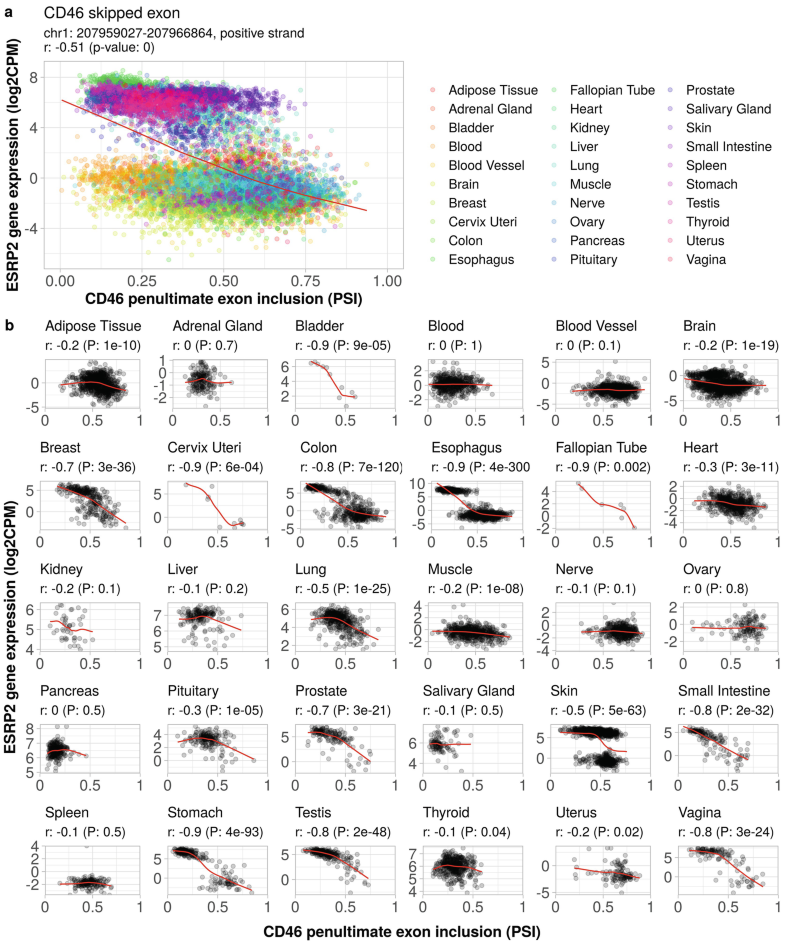
\includegraphics[width=1\textwidth]{images/psichomics/8-gtex-cor}
  \centering
  \caption[\emph{ESRP2} expression versus \emph{CD46} penultimate exon PSI in GTEx]{\textbf{Scatterplots of normalised \emph{ESRP2} expression versus PSI values for \emph{CD46} penultimate exon inclusion across GTEx tissues, altogether (a) and by tissue (b).} For each plot, the red line illustrates the fitted Loess regression curve. The Pearson’s correlation coefficients (\emph{r}) and associated p-values (P) are shown.}
  \label{fig:psichomics-gtex-cor}
\end{figure}

\begin{figure}[!p]
  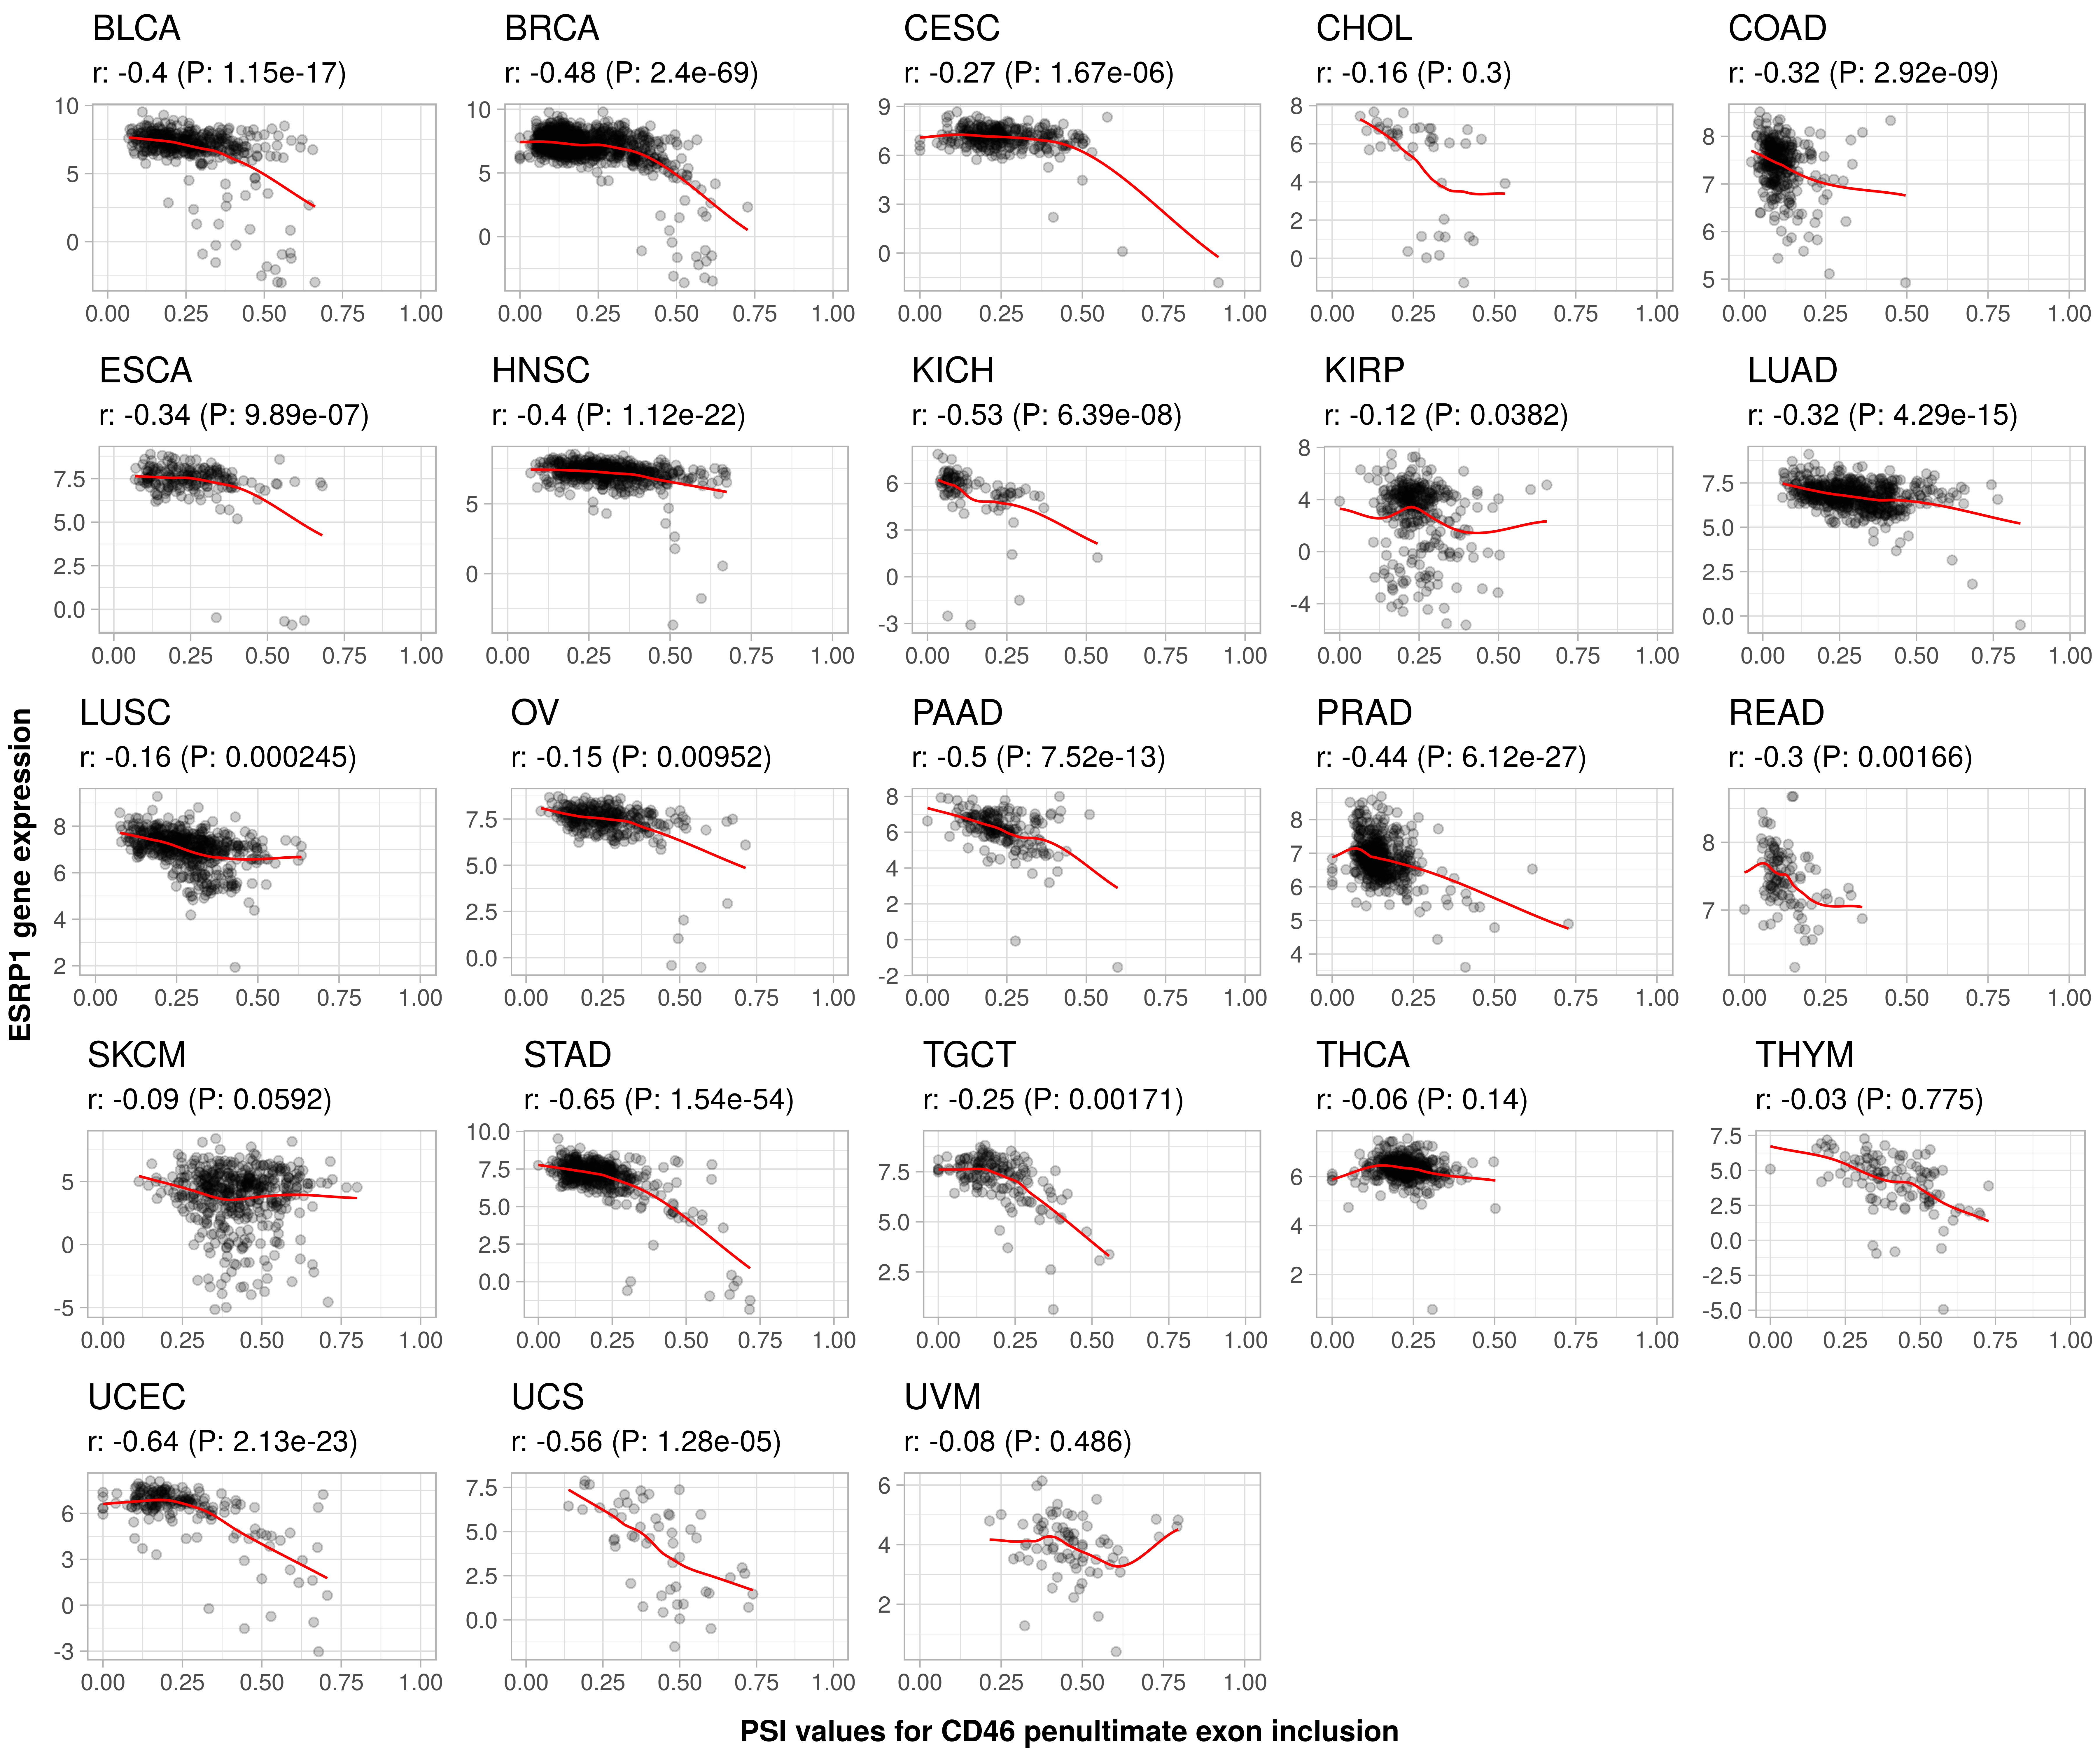
\includegraphics[width=1\textwidth]{images/psichomics/9-tcga-esrp1}
  \centering
  \caption[\emph{ESRP1} expression versus \emph{CD46} penultimate exon PSI in TCGA]{\textbf{Scatterplots of normalised \emph{ESRP1} expression versus PSI values for \emph{CD46} penultimate exon inclusion across TCGA tumour types.} For each plot, the red line illustrates the fitted Loess regression curve. The Pearson’s correlation coefficients (\emph{r}) and associated p-values (P) are shown.

\hspace{\textwidth}

\textsmaller{\textbf{Legend:} ACC adrenocortical carcinoma, BCLA urothelial bladder carcinoma, BRCA breast invasive carcinoma, CESC cervical squamous cell carcinoma and endocervical adenocarcinoma, CHOL cholangiocarcinoma, COAD colon adenocarcinoma, DLBC lymphoid neoplasm diffuse large B-cell lymphoma, ESCA esophageal carcinoma, GBM glioblastoma multiforme, HNSC head and neck squamous cell carcinoma, KICH kidney chromophobe, KIRC kidney renal clear cell carcinoma, KIRP kidney renal papillary cell carcinoma, LGG brain lower grade glioma, LIHC liver hepatocellular carcinoma, LUAD lung adenocarcinoma, LUSC lung squamous cell carcinoma, MESO mesothelioma, OV ovarian serous cystadenocarcinoma, PAAD pancreatic adenocarcinoma, PCPG pheochromocytoma and paraganglioma, PRAD prostate adenocarcinoma, READ rectum adenocarcinoma, SARC sarcoma, SKCM skin cutaneous melanoma, STAD stomach adenocarcinoma, TGCT testicular germ cell tumours, THCA thyroid carcinoma, THYM thymoma, UCEC uterine corpus endometrial carcinoma, UCS uterine carcinosarcoma, UVM uveal melanoma.}
}
  \label{fig:psichomics-tcga-esrp1}
\end{figure}

\begin{figure}[!ht]
  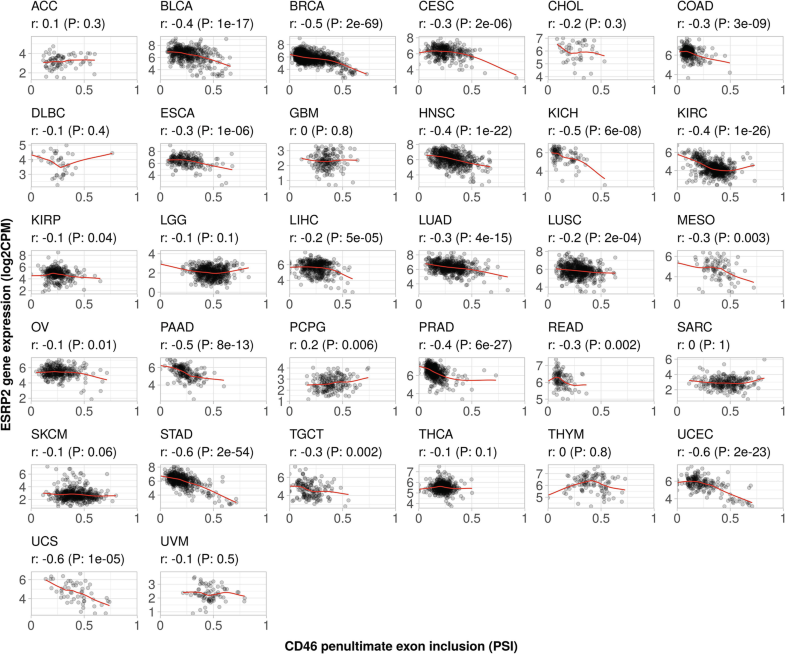
\includegraphics[width=1\textwidth]{images/psichomics/10-tcga-esrp2}
  \centering
  \caption[\emph{ESRP2} expression versus \emph{CD46} penultimate exon PSI in TCGA]{\textbf{Scatterplots of normalised \emph{ESRP2} expression versus PSI values for \emph{CD46} penultimate exon inclusion across TCGA tumour types.} For each plot, the red line illustrates the fitted Loess regression curve. The Pearson’s correlation coefficients (\emph{r}) and associated p-values (P) are shown. See caption of \shortref{fig:psichomics-tcga-esrp1} for legend.}
  \label{fig:psichomics-tcga-esrp2}
\end{figure}

\subsubsection{Pancancer prognostic value of the skipping of \emph{CD46} penultimate exon}

The prognostic value of a given alternative splicing event (or gene) may be evaluated by separating subjects based on a PSI cutoff for a given alternative splicing event (or expression cutoff for a given gene). The survival differences are then log-rank tested based on Kaplan-Meier estimators.

We performed overall survival analysis by selecting right data censoring\footnote{psichomics supports left, right, and interval data censoring for survival analysis. Events may occur after the last observation (right censoring, such as in the case of subjects having no event reported during the study or dropping from it altogether), before an observation is performed (left censoring, for instance when events happened in an uncertain time before the start of the study) or in-between observations (interval censoring, such as when patients require periodic follow-ups and the time of an event occurrence falls between follow-ups but is not certain) \cite{zhang:2010wk}.}, follow-up time as days to death and the event of interest as death. Analysing days to death as the follow-up time and death as the event of interest is known as an overall survival analysis, that is, the study of the time until the subject’s death following diagnosis. For patients whose days to death are not available, the follow-up time is based on days to last follow-up (otherwise, these subjects would be discarded from the analyses)\footnote{We recommend using days to death (complemented with days to last follow-up for missing values) as follow-up time when using TCGA data. Days to last follow-up are sometimes lower or completely missing relative to days of death, which would result in discarding individuals from the analysis.}.
 
In this context, we used clinical and transcriptomic data from TCGA to evaluate the prognostic value of the skipping of \emph{CD46} penultimate exon based on overall survival curves across TCGA tumour types to compare tumour samples with low and high inclusion of the \emph{CD46} penultimate exon. A $-log_{10}(\textrm{p-value})$ plot by cutoff displays the p-values of the log-rank test of survival across multiple PSI cutoffs for the selected alternative splicing event. The PSI cutoff maximising the significance of the survival difference is automatically selected. The splicing of \emph{CD46} penultimate exon seems to have prognostic value in select cancer types, such as brain lower-grade glioma and lung adenocarcinoma (\shortref{fig:psichomics-cd46-as-prognosis}).

% \footnote{If the PSI cutoff suggested by psichomics has unbalanced number of subjects between groups (e.g., in \shortref[d]{fig:psichomics-cd46-as}, the lowest log-rank p-value corresponds to a comparison of 1 versus 506 subjects), we should use another cutoff with more reasonably balanced groups and for which the p-value is still significant. Sample size calculations can be performed based on test assumptions (e.g., probability of failure for each group during the study) using existing R packages, such as \emph{powerSurvEpi} \cite{qiu:2021wd}.}

\begin{figure}[!ht]
  \begin{overpic}[abs,width=.8\textwidth]{images/psichomics/11-cd46-as-prognosis}
    	\put(5,175){\colorbox{white}{\textsf{\textbf{a}}}}
		\put(185,175){\colorbox{white}{\textsf{\textbf{b}}}}
	  	\put(5,35){\colorbox{white}{\textsf{\textbf{c}}}}
		\put(185,35){\colorbox{white}{\textsf{\textbf{d}}}}
  \end{overpic}
  \centering
  \caption[Prognostic value of \emph{CD46} penultimate exon inclusion]{\textbf{Prognostic value of \emph{CD46} penultimate exon inclusion across select TCGA cancer types.} (a, b) Kaplan-Meier plots of overall survival for all patients stratified by the respective alternative splicing event’s PSI cutoff that maximised the significance of differences in survival between patient groups with a reasonable number of subjects within each group. Each patient was assigned the PSI value of their tumour sample(s). (c, d) Log-rank’s $-log_{10}(\textrm{p-value})$ plot by PSI cutoff. Note that in panel d, for PSI values around 0.8, there are high log-rank $-log_{10}(\textrm{p-value})$ although only one individual is being compared against 506 subjects. Legend: LGG brain lower grade glioma, LUAD lung adenocarcinoma.}
  \label{fig:psichomics-cd46-as-prognosis}
\end{figure}

\subsection{Time benchmarking}

The runtimes required to load, quantify and analyse data from different TCGA (data version \texttt{2016\_01\_28} from FireBrowse) and GTEx v7 cohorts were benchmarked. The breast cancer cohort contains the highest number of RNA-seq samples in TCGA, thus being the cohort for which takes more time to load, quantify and analyse alternative splicing and gene expression data. Contrastingly, processed data from GTEx come bundled in files containing all tissues. Although only data from specified tissues are loaded, scanning though the large GTEx file still delays data loading. Tissues from GTEx were loaded in pairs for subsequent differential splicing analyses (\shortref[A]{fig:psichomics-performance}).

\begin{figure}[!ht]
  \begin{overpic}[abs,width=\textwidth]{images/psichomics/performance-benchmark}
  	\put(0,148){\colorbox{white}{\textsf{\textbf{a}}}}
  	\put(220,148){\colorbox{white}{\textsf{\textbf{b}}}}
  \end{overpic}
  \centering
  \caption[Performance benchmark for alternative splicing analysis]{\textbf{Performance benchmark for alternative splicing analysis using RNA-seq data from multiple TCGA and GTEx sample types.} (a) Median times of 10 runs of data loading, gene expression (GE) normalisation, skipped exon (SE) event quantification and differential expression and splicing analysis (normal versus tumour for TCGA data or pairwise tissue comparison for GTEx data) using psichomics. The default settings were used during the runs. (b) Estimation of the time complexity of each of the aforementioned steps in psichomics. Randomly generated synthetic datasets of different sample size s were used as input. Equations and coefficient of determination ($R^2$) for the best fits are displayed.}
  \label{fig:psichomics-performance}
\end{figure}

Synthetic datasets for gene expression and exon-exon junction quantification of multiple sample sizes were generated, based on TCGA data distributions, to determine the time complexity of each step in psichomics as a function of the number of input samples $s$ (\shortref[B]{fig:psichomics-performance}). Assuming a constant number of genes (20 000 in the benchmark) or exon-exon junctions (200 000), the time taken to load data grows quadratically with $s$. Gene expression normalisation and differential expression are based on commonly-used, time-efficient bioinformatics tools and the times taken for each also grow quadratically with $s$. Alternative splicing quantification is associated with element-wise operations on matrices of dimensions $s$ by the number of alternative splicing events and takes a runtime approximately proportional to the square of $s$, for a given number of alternative splicing events (around 9000 for each benchmarked run). Finally, differential splicing is based on multiple, distinct statistical analyses of alternative splicing quantification data and grows linearly with $s$.

\subsection{Alternative splicing quantification benchmarking}

Although jSplice's \cite{christinat:2016ui} and DIEGO’s \cite{doose:2018uv} splicing quantifications rely on junction read counts, their alternative splicing module expression and junction usage metrics, respectively, are not directly comparable with psichomics’ PSI values. To evaluate their accuracy in the absence of any known tool with the same input (junction read counts) and output metric (PSI) as psichomics, psichomics-estimated PSI values were compared to those estimated by RT-PCR and using VAST-TOOLS \cite{irimia:2014wt} across multiple tissue and cell line samples from human, mouse and chicken \cite{tapial:2017ui}. VAST-TOOLS follows an analogous, and therefore more directly comparable, procedure for computing PSI values and there is a substantial overlap between the alternative splicing event annotations used by the two tools. psichomics estimates highly correlate with both others, particularly for mouse and human (\shortref{fig:psi-comparison}), suggesting robustness and reproducibility in alternative splicing quantification by psichomics. Of note, the lower correlation for chicken samples is attributable to a single outlier, as its removal increases the correlation coefficients between psichomics and RT-PCR estimates (Pearson's \emph{r} = 0.87, p-value $< 0.01$; Spearman's \emph{rho} = 0.87, p-value $< 0.01$) and psichomics and VAST-TOOLS estimates (Pearson's \emph{r} = 0.93, p-value $< 0.01$; Spearman's \emph{rho} = 0.94, p-value $< 0.01$).

\begin{figure}[!ht]
  \begin{overpic}[abs,width=\textwidth]{images/psichomics/psi-comparison}
  	\put(0,157){\colorbox{white}{ }}
  	\put(146,157){\colorbox{white}{ }}
  	\put(296,157){\colorbox{white}{ }}
  \end{overpic}
  \centering
  \caption[Comparison between PSI values estimated by psichomics, VAST-TOOLS and RT-PCR]{\textbf{Comparison between PSI values estimated by psichomics, VAST-TOOLS and RT-PCR} across multiple tissue and cell line samples from human, mouse and chicken. Pearson’s (\emph{r}) and Spearman’s (\emph{rho}) correlation coefficients and respective p-values are shown. Linear regression lines are coloured per species with the respective 95\% confidence interval represented as their shades. Identity line in orange.}
  \label{fig:psi-comparison}
\end{figure}

To assess the influence of RNA-seq read coverage on psichomics PSI estimates, different numbers of junction reads per event were simulated for different given PSI values (10 000 times for each combination). \shortref{fig:psichomics-accuracy} shows that the accuracy of PSI estimation by psichomics is expectedly sensitive to junction read coverage, particularly for intermediate PSI values, with 90\% prediction intervals $<0.1$ for coverage higher than a few hundred reads.

\begin{figure}[!ht]
  \begin{overpic}[abs,width=\textwidth]{images/psichomics/psichomics-accuracy}
      	\put(-5,237){\colorbox{white}{\textsf{\textbf{a}}}}
	  	\put(219,237){\colorbox{white}{\textsf{\textbf{b}}}}
		\put(-5,115){\colorbox{white}{\textsf{\textbf{c}}}}
		\put(219,115){\colorbox{white}{\textsf{\textbf{d}}}}
  \end{overpic}
  \centering
  \caption[Event read coverage on accuracy of psichomics PSI quantification]{\textbf{Dependence of accuracy of psichomics PSI quantification on event read coverage.} (a) Comparison between simulated "real" PSI values and the mean, 95th percentile and 5th percentile of their corresponding PSI estimates for different simulated numbers of junction reads. (b) 90\% prediction interval (i.e., difference between the 95th and the 5th percentiles) across different number of junction reads for simulated "real" PSI values. (c,d) Density plots of PSI estimates for each simulated "real" PSI and junction read coverage combination (except those involving PSI $= 0$ and PSI $= 1$). Each "real" PSI and junction read coverage combination was simulated 10 000 times.}
  \label{fig:psichomics-accuracy}
\end{figure}


Alternative splicing events annotated by TCGASpliceSeq \cite{ryan:2016tm}, an online tool that displays pre-computed PSI values across multiple TCGA tumour types, were matched to those from psichomics based on their genomic coordinates. In total, 321 183 of 757 749 (42\%) skipped exon, 70 837 of 126 725 (56\%) alternative 5$'$ splice site and 90 940 of 155 799 (58\%) alternative 3$'$ splice site events were successfully matched. When available from both programs, PSI estimates for each of the 482 960 alternative splicing events in each of the 9 913 matched samples were compared between TCGASpliceSeq and psichomics, being highly correlated (N = 92 444 302; Pearson's \emph{r} = 0.97, p-value $< 10^{15}$; Spearman's \emph{rho} = 0.94, p-value $< 10^{15}$; \shortref{fig:tcgaspliceseq-correlation}).

\begin{figure}[!ht]
  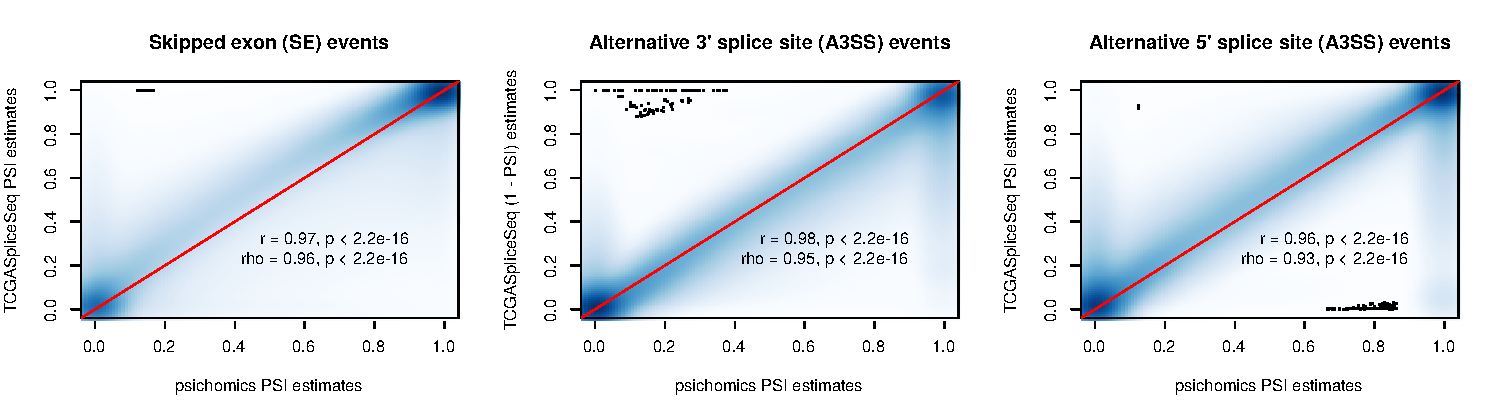
\includegraphics[width=1\textwidth]{images/psichomics/tcgaspliceseq-correlation}
  \centering
  \caption[Correlation of PSI estimates between TCGASpliceSeq and psichomics]{\textbf{Correlation of PSI estimates for TCGA samples between TCGASpliceSeq and psichomics.} For A3SS events, PSI values from psichomics correspond to $1 – \textrm{PSI}$ from TCGASpliceSeq (the splice site deemed as alternative in A3SS events by TCGASpliceSeq is constitutive in psichomics and vice-versa). Pearson’s (\emph{r}) and Spearman’s (\emph{rho}) correlation coefficients and respective p-values are shown. Identity line in red.}
  \label{fig:tcgaspliceseq-correlation}
  \vspace{-\intextsep}
\end{figure}

%\subsection{Impact}

%There are multiple ways to measure the impact of psichomics. First, we can check the metrics surrounding the article itself. 

% importance of maintaining software and replying to user feedback

%- Invitation to write a book chapter

%Although there is no direct way to measure user engagement with psichomics, we can track:

%- Bioconductor downloads

%- Docker Hub image downloads 

%- visitors to the official psichomics documentation

%- visitors to the website

%- feedback via GitHub issues and emails

%- citations

%It is wonderful to see that the work I put into psichomics is appreciated based on feedback received via GitHub and email. psichomics is still used nowadays based on citations from recent published articles (Ling et al., 2020; Baeza-Centurion et al., 2020; Birladeanu et al., 2021). In the lab, we can also track visitors of psichomics’ documentation via Google Analytics to better understand our users (e.g., what pages they visit the most).

\section{Conclusion}

Alternative splicing is a regulated molecular mechanism involved in multiple cellular processes and its dysregulation has been associated with diverse pathologies \cite{kelemen:2013tc,paronetto:2016vw,wang:2008wa,oltean:2014vm}. The advent of next-generation sequencing technologies has allowed the investigation of transcriptomes of human biological samples to be expanded to alternative splicing. RNA-seq data, like those yielded by the GTEx and TCGA projects, are indeed playing crucial role in the improvement of our insights into the role of alternative splicing in both physiological and pathological contexts \cite{paronetto:2016vw,wang:2008wa,gallego-paez:2017wc,tsai:2015ve,danan-gotthold:2015ut}).

However, the most commonly used tools for alternative splicing analyses currently do not allow researchers to fully benefit from the wealth of pre-processed RNA-seq data made publicly available by the aforementioned projects. For instance, they lack support for estimating PSIs based on splice junction read counts. Such functionality would allow users to overcome the difficulties caused by the raw RNA-seq data from GTEx and TCGA being under controlled access and, more importantly, their processing requiring computational resources inaccessible to the majority of research labs. psichomics thus exploits pre-processed alternative splicing annotation and exon–exon junction read count data from TCGA and GTEx, two of the richest sources of molecular information on human tissues in physiological and pathological conditions, as well as recount2 and user-owned data, allowing researchers to hasten alternative splicing quantification and subsequent analyses by avoiding the time-consuming alignment of RNA-seq data to a genome or transcriptome of reference followed by splice junction detection.

Together with support for the integration of molecular and sample-associated clinical information, the group creation functionalities featured in psichomics ensure full customisability of data grouping for downstream analyses. Interesting groups to compare in TCGA, for instance, may range from the simple contrast between reformed and current smokers in lung cancer to complex combinations of gender, race, age, country and other subject attributes across multiple cancers. When survival data are available, survival analyses can be performed on samples by PSI or gene expression levels, thereby assessing the putative prognostic value of a respective molecular feature.

%\textcolor{red}{The integrative analysis of publicly available TCGA data by psichomics allowed us to identify multiple exons differentially spliced between breast tumour stage I and normal samples, therefore deeming them potential diagnostic biomarkers, and to assess their putative prognostic value. The output of psichomics is validated by identified alternative splicing alterations that have been previously linked to the disease, including events in RPS24, NUMB, FBLN2 and AP2B1. Previously understudied, yet intriguing, events were also identified, such as the skipping of SLMAP exon 23 and UHRF2 exon 10. These may provide novel insights into the early stages of breast cancer development.} Indeed, it is of utmost importance to foster alternative splicing analyses of clinical samples as a crucial complement to more conventional research focused on total gene expression.

To ensure researchers with different skills can take the most out of psichomics, we added an intuitive and more accessible graphical interface, while still supporting a command-line interface. psichomics has recently been deployed online at \alink{compbio.imm.medicina.ulisboa.pt/psichomics}\footnote{More information in \fullref{chap:app-server}.} to allow the on-demand use of the latest version of psichomics with no installation required, levering the intuitive graphical interface to make alternative splicing analyses more enticing to less computationally-inclined biomedical researchers.

Notwithstanding its merits, psichomics only quantifies alternative splicing events based on exon–exon junction read counts, limiting the types of alternative splicing events profiled. For instance, exon–intron junction, exon body and intron body quantifications are vital to confirm intron retention and alternative 5$'$ and 3$'$ UTR events over further transcriptional variations \cite{braunschweig:2014tr}.
However, although GTEx (but neither TCGA nor recount2) readily provides intron and exon body read quantification for retrieval, none provides exon–intron junction quantification. To overcome this, psichomics allows to import alternative splicing events quantified from other programs, including VAST-TOOLS that quantifies intron retention events.

Another limitation is psichomics' reliance on existing alternative splicing event annotations and an on the pre-processing of RNA-seq data by third-party pipelines (as is the case for GTEx, TCGA and recount2), depriving the user of the flexibility to identify \emph{de novo} alternative splicing events. Even so, when FASTQ or BAM files are accessible, psichomics supports the loading of alternative splicing annotations generated by different programs that take those files as input, namely rMATS \cite{shen:2014tk}, which is able to generate \emph{de novo} annotations\footnote{More information in \alink{nuno-agostinho.github.io/psichomics/articles/AS_events_preparation}.}.

% \textcolor{red}{Using psichomics, we are able not only to identify novel exons differentially spliced between tumour stage I and normal breast samples but also to pinpoint potentially clinically relevant splicing events by embracing clinical data and evaluating their prognostic value.}
% For future iterations of psichomics, potentially support recount3?

Since its publication, psichomics has been used to analyse alternative splicing in multiple scientific articles, such as \cite{coomer:2019wz,baeza-centurion:2019tb,munkley:2019wr,baeza-centurion:2020vb}. Based on these citations and positive user feedback, we believe that fellow researchers and clinicians are able to intuitively employ psichomics to assist them in uncovering novel splicing-associated prognostic factors and therapeutic targets, as well as in advancing our understanding of how alternative splicing is regulated in physiological and disease contexts.

% !TEX root = ../PhD Thesis.tex

%\chapter{cTRAP: identification of candidate causal perturbations from differential gene expression data}
\chapter{cTRAP}
\label{chap:ctrap}

\begin{figure}[!b]
  \vspace*{-1cm}
  \includegraphics[width=.96\textwidth]{images/cTRAP/screenshot}
  \centering
  \vspace*{-.5cm}
  \caption[cTRAP screenshot]{\textbf{cTRAP screenshot} (21 Dec 2021).}
  \label{fig:cTRAP-screenshot}
\end{figure}

During a stormy day in our 2017 Madeira Lab retreat, we had a brainstorm to discuss the unique propositions that the lab could provide to the scientific community. One idea that emerged was to make it easier to identify putative causal perturbations by comparing a custom differential gene expression against the large-scale database of differential expression profiles from CMap \cite{subramanian:2017ul}, a repository of transcriptomic signatures for thousands of genetic (gene overexpression or knockout) and pharmacological perturbations in human cancer cell lines. % This kind of analysis is available in CMap's web apps at \alink{clue.io} \cite{subramanian:2017ul}, but their results are difficult to integrate in downstream analyses, suffer from poor API documentation for programatic access and lack basic visualisation tools.

% clue.io does indeed allow for batch query: https://clue.io/connectopedia/batch_query_tutorial
% clue.io API's is not straightforward: https://clue.io/connectopedia/query_api_tutorial

We thus developed cTRAP, an R package and web app to compare user-provided differential gene expression profiles with the perturbations available from CMap, allowing to infer putative candidate molecular causes for the observed differences, as well as compounds that may promote or revert them (\shortref{fig:cTRAP-screenshot}).

After releasing the first version in Bioconductor, multiple features were added (\shortref{tab:cTRAP}). Inspired by the method used to compare gene expression changes against the CMap database, we also added a way to predict targeting drugs by using drug sensitivity datasets that featured gene expression for multiple genes in many cell lines. Additionally, cTRAP also allows to analyse the enrichment of molecular descriptors for compounds from NCI60 and CMap. More recently, we developed a visual interface to host cTRAP online with support for user sessions and background tasks.

\begin{table}[!ht]
\parnotereset
\small
\caption[Major cTRAP milestones]{\textbf{Major cTRAP milestones.}}
\label{tab:cTRAP}
\begin{tabularx}{\textwidth}{ r r l }
\toprule
\textbf{Version} & \textbf{Release date} & \textbf{Main features} \\
\midrule
1.0.0  &  2 Nov 2018 & Compare differential expression profiles against CMap data\parnote{First Bioconductor release.} \\
\multirow{2}*{1.4.0}  & \multirow{2}*{12 Nov 2019} & Predict targeting drugs using NCI60, CTRP and GDSC data \\
       &             & Analyse drug set enrichment using molecular descriptors \\
1.8.0  & 30 Oct 2020 & Include graphical functions to load data and analyse results \\
1.10.0 & 20 May 2021 & Improve speed and memory usage when comparing data \\
1.12.0 & 28 Oct 2021 & Add web server support (optimised to run in ShinyProxy)\parnote{First version available online.} \\
\bottomrule
\end{tabularx}
\parnotes
\end{table}

The associated cTRAP manuscript (of which I am a co-first and co-corresponding author) is in preparation for submission to an international peer-reviewed scientific journal and shares similarities with this chapter.

\section{Background}

The Connectivity Map (CMap) is a repository of transcriptomic signatures of thousands of genetic and pharmacological perturbations in human cancer cell lines \cite{subramanian:2017ul}. Comparing differential gene expression profiles with those from CMap allows to infer putative molecular causes for the observed differences, as well as compounds that may promote or revert those changes.

The CMap and LINCS Unified Environment (\alink{clue.io}) was developed as a collection of user-friendly tools for the manipulation of CMap data and their integration with user-provided data \cite{subramanian:2017ul}. However, \alink{clue.io} limits the maximum number of input genes for CMap queries, expresses results' significance in a non-standard significance score, is difficult to automate for downstream analyses and does not support using local computing resources. Furthermore, \alink{clue.io} does not currently integrate with drug sensitivity datasets, which could further assist in pinpointing compounds that selectively target cells.

We thus developed cTRAP, an R package and web app that identifies potentially causal molecular perturbations by seamlessly comparing full user-provided differential gene expression results with those available from CMap. cTRAP also supports comparisons with gene expression/drug sensitivity associations derived from the NCI-60 \cite{shoemaker:2006wi}, the Cancer Therapeutics Response Portal (CTRP) \cite{seashore-ludlow:2015ws} and the Genomics of Drug Sensitivity in Cancer (GDSC) \cite{yang:2012vk}, to identify compounds that could target the phenotypes associated with the user-provided differential expression profiles. In cTRAP, similarity between differential gene expression results is measured by gene set enrichment \cite{subramanian:2017ul,subramanian:2005wu} and correlation scores.

cTRAP is available online as a web app at \alink{compbio.imm.medicina.ulisboa.pt/cTRAP}, but can be locally installed using Bioconductor (\alink{bioconductor.org/packages/cTRAP}) or Docker (\dockerlink{nunoagostinho/ctrap}). The source code of cTRAP is available at \alink{github.com/nuno-agostinho/cTRAP}.

\section{Materials and methods}

\begin{figure}[!b]
  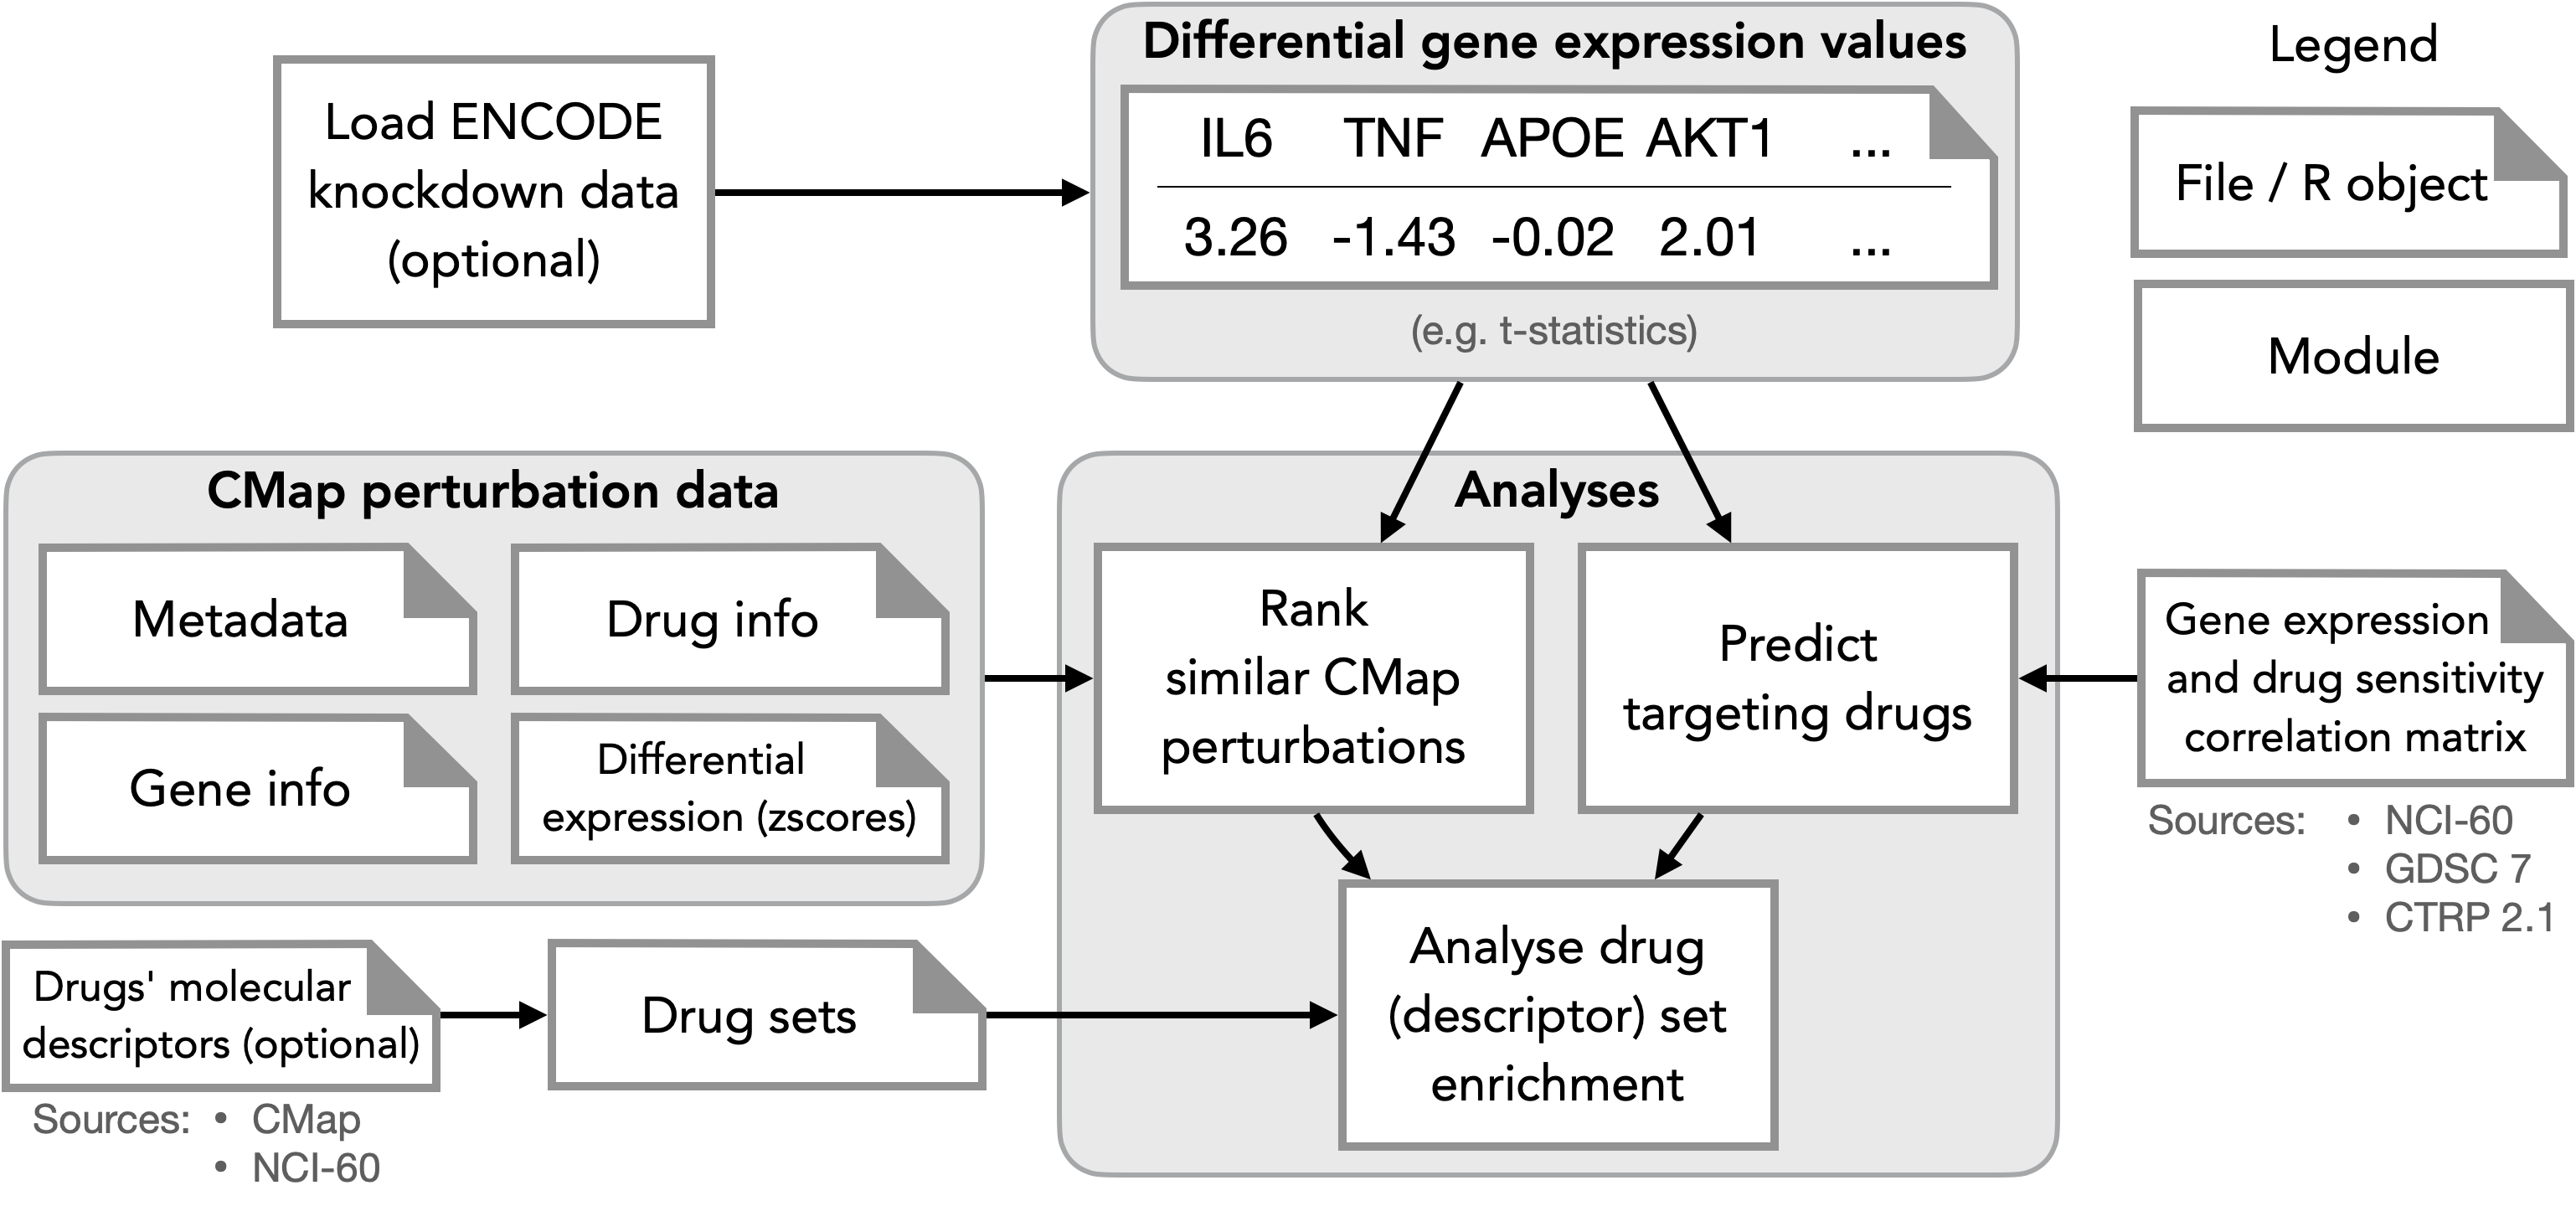
\includegraphics[width=.8\textwidth]{images/ctrap/workflow}
  \centering
  \caption[cTRAP workflow]{\textbf{cTRAP workflow.} cTRAP allows to perform three analyses: \textbf{(1) rank similar CMap perturbations} by comparing user-provided differential gene expression values against CMap perturbation data, \textbf{(2) predict targeting drugs} by comparing user-provided differential gene expression values against correlation matrices of gene expression and drug sensitivity data and \textbf{(3) analyse drug (descriptor) set enrichment} using drug sets and the results from either the first or second analysis. CMap perturbation data, gene expression/drug sensitivity correlation matrices and drug molecular descriptors for drug sets can be automatically downloaded.}
  \label{fig:ctrap-workflow}
\end{figure}

From a vector of user-provided differential expression results (e.g. t-statistic values) with respective gene symbols, cTRAP can return a ranked list of similar CMap perturbations or predict targeting drugs. Moreover, cTRAP can also analyse the enrichment of drug sets in an ordered vector of compounds to identify common compound characteristics (Figures \shorterref{fig:ctrap-workflow} and \shorterref{fig:ctrap-file-structure}).

\begin{figure}[!ht]
  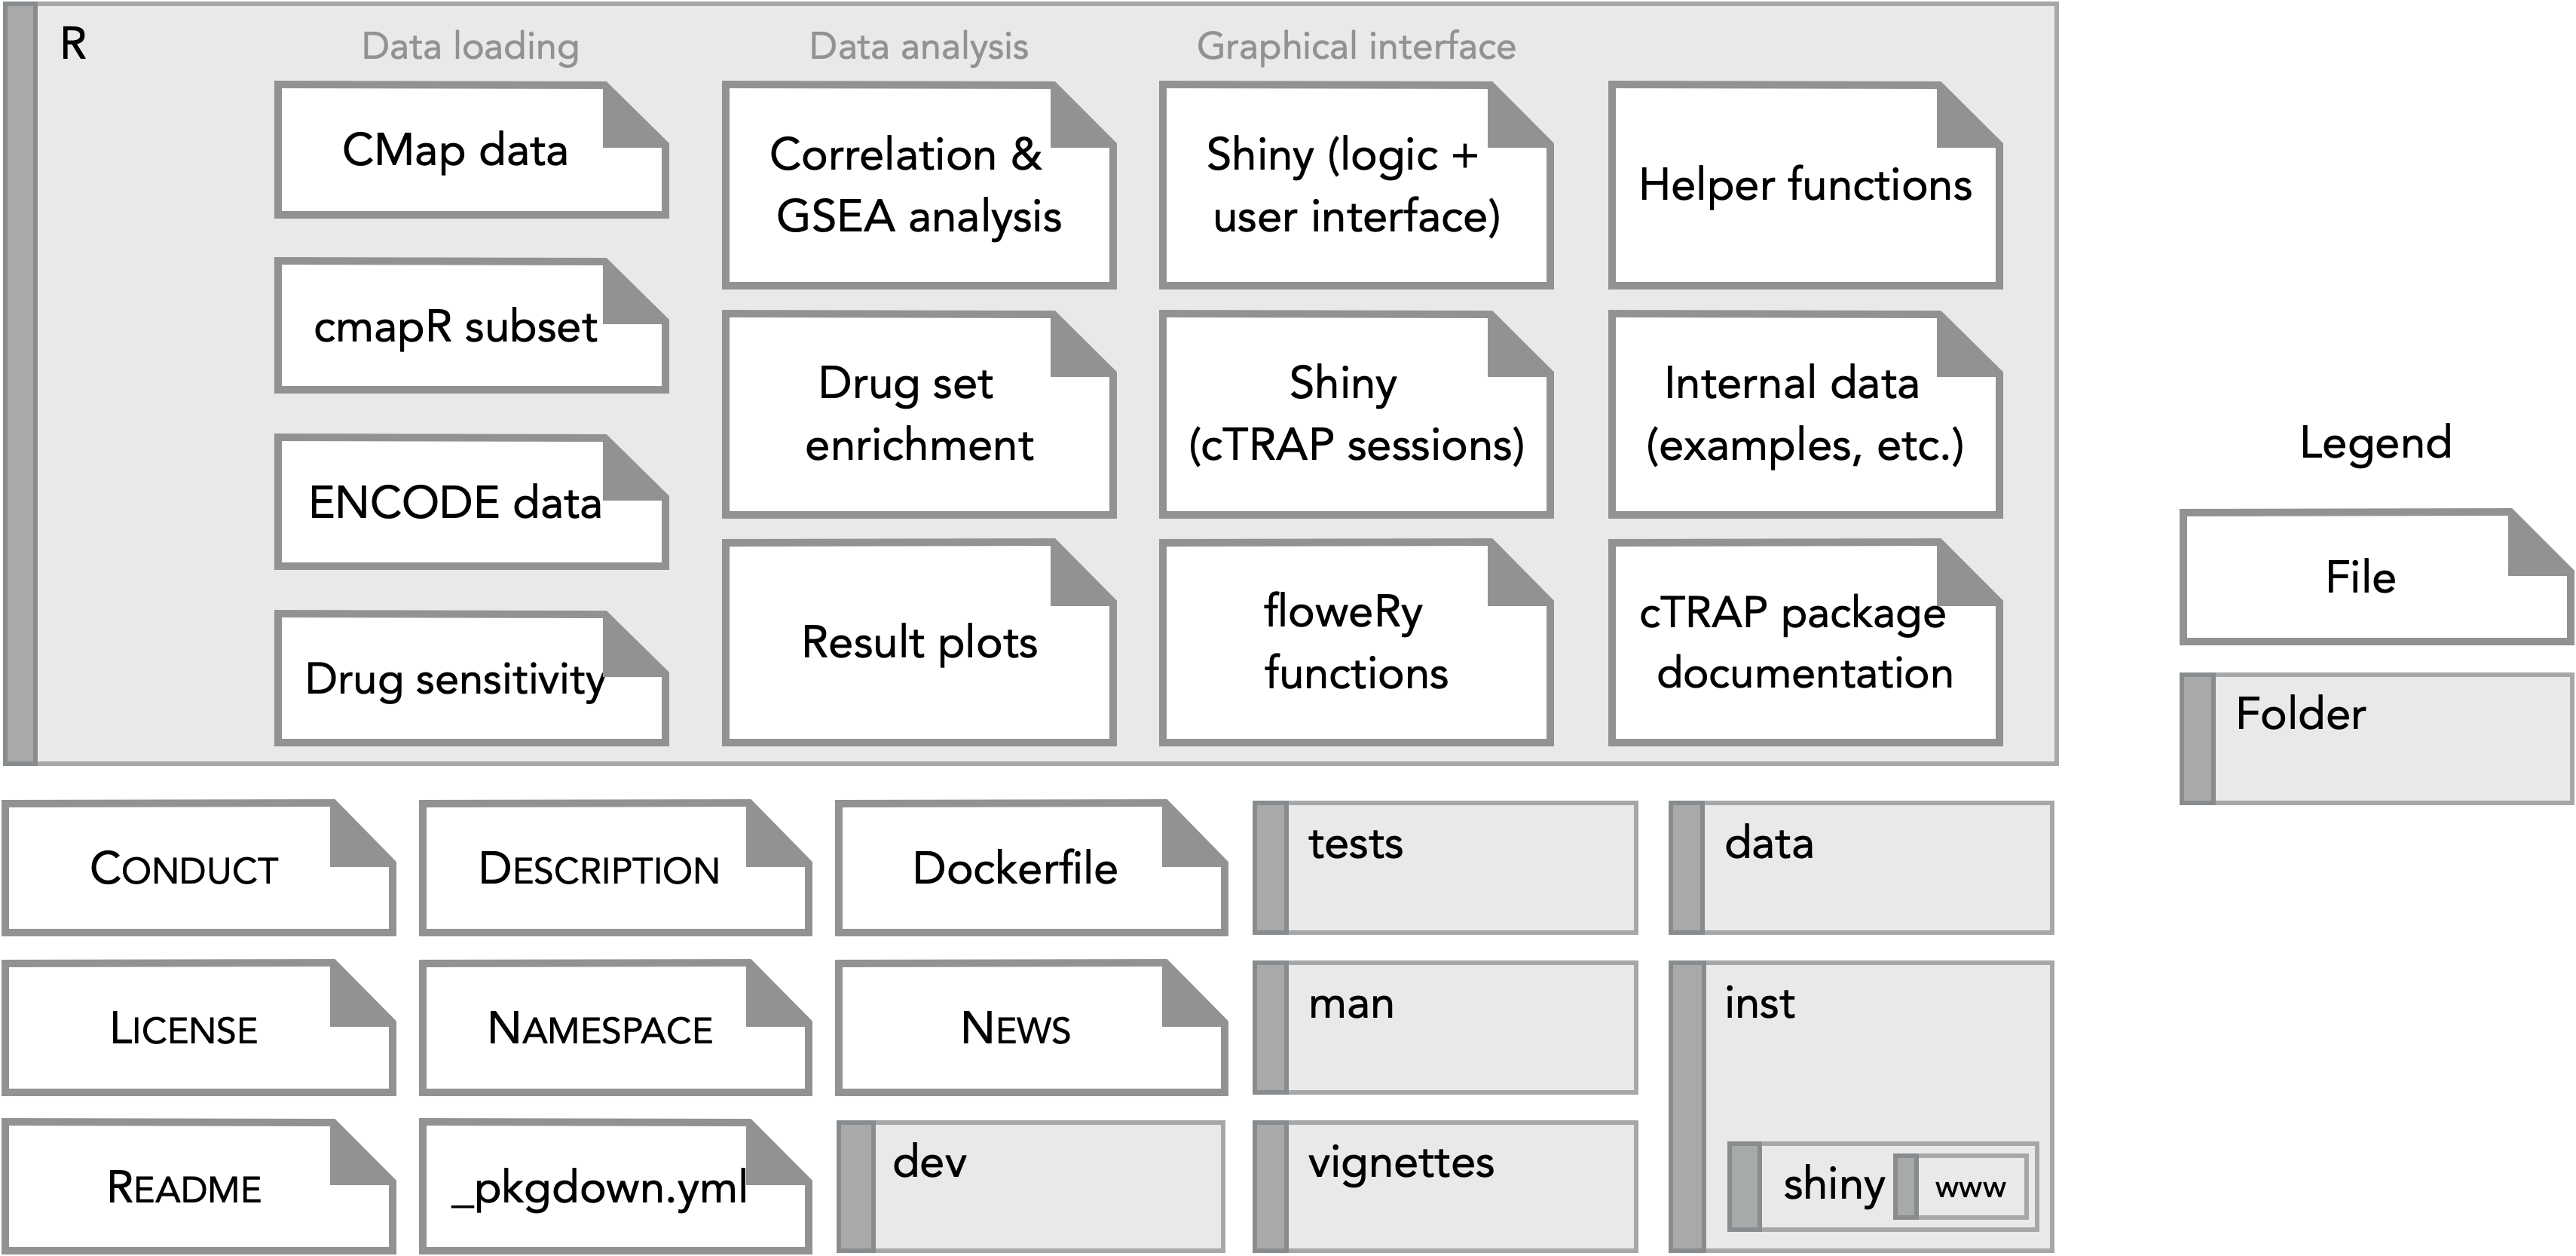
\includegraphics[width=1\textwidth]{images/ctrap/file-structure}
  \centering
  \caption[cTRAP file structure]{\textbf{Visual representation of cTRAP's file structure.} As usual in an R package, the \texttt{R} folder contains the scripts with cTRAP functions and data. \texttt{dev} is a custom folder that stores supporting scripts (e.g. test workflows and benchmarks); its contents are not included when building the R package.}
  \label{fig:ctrap-file-structure}
\end{figure}

\subsection{ENCODE knockdown data}

Using cTRAP, we can query and download ENCODE knockdown (and respective control) samples for multiple cell lines, filter low coverage counts from gene expression data, convert from ENSEMBL identifiers to gene symbol, and perform differential gene expression using \texttt{voom()}, \texttt{lmFit()} and \texttt{eBayes()} from the \texttt{limma} R package \cite{ritchie:2015tm}. First, \texttt{voom()} is used with the \emph{quantile} normalisation to transform count data to log\textsubscript{2} CPM (counts per million) and estimate the mean-variance relationship to compute weights used in linear modelling. Gene-wise linear models are then fitted using \texttt{lmFit()} between the knockdown and the control samples, followed by moderated t-tests and the calculation of log-odds of differential expression, using \texttt{eBayes()} for empirical Bayes moderation of standard errors.

cTRAP includes an example dataset (\texttt{diffExprStat}) with the differential gene expression results (t-statistic values) between the EIF4G1 knockdown in HepG2 versus control (\shortref{lst:diffExprStat}).

\begin{lstlisting}[caption=Code to obtain example dataset \texttt{diffExprStat}.,language=R,label={lst:diffExprStat}]
library(cTRAP)
ENCODEmetadata <- downloadENCODEknockdownMetadata(cellLine="HepG2",
                                                  gene="EIF4G1")
ENCODEsamples  <- loadENCODEsamples(ENCODEmetadata)[[1]]
counts         <- prepareENCODEgeneExpression(ENCODEsamples)

# Remove low coverage genes (>= 10 counts shared by >= 2 samples)
minReads   <- 10
minSamples <- 2
filter     <- rowSums(counts[ , -c(1, 2)] >= minReads) >= minSamples
counts     <- counts[filter, ]

# Convert ENSEMBL identifiers to gene symbols
counts$gene_id <- convertGeneIdentifiers(counts$gene_id)

# Perform differential gene expression (DGE) analysis
diffExpr <- performDifferentialExpression(counts)

# Get t-statistic values of DGE and respective gene names
diffExprStat <- diffExpr$t
names(diffExprStat) <- diffExpr$Gene_symbol
\end{lstlisting}

\subsection{Ranking of similar CMap perturbations}

\begin{figure}[!b]
  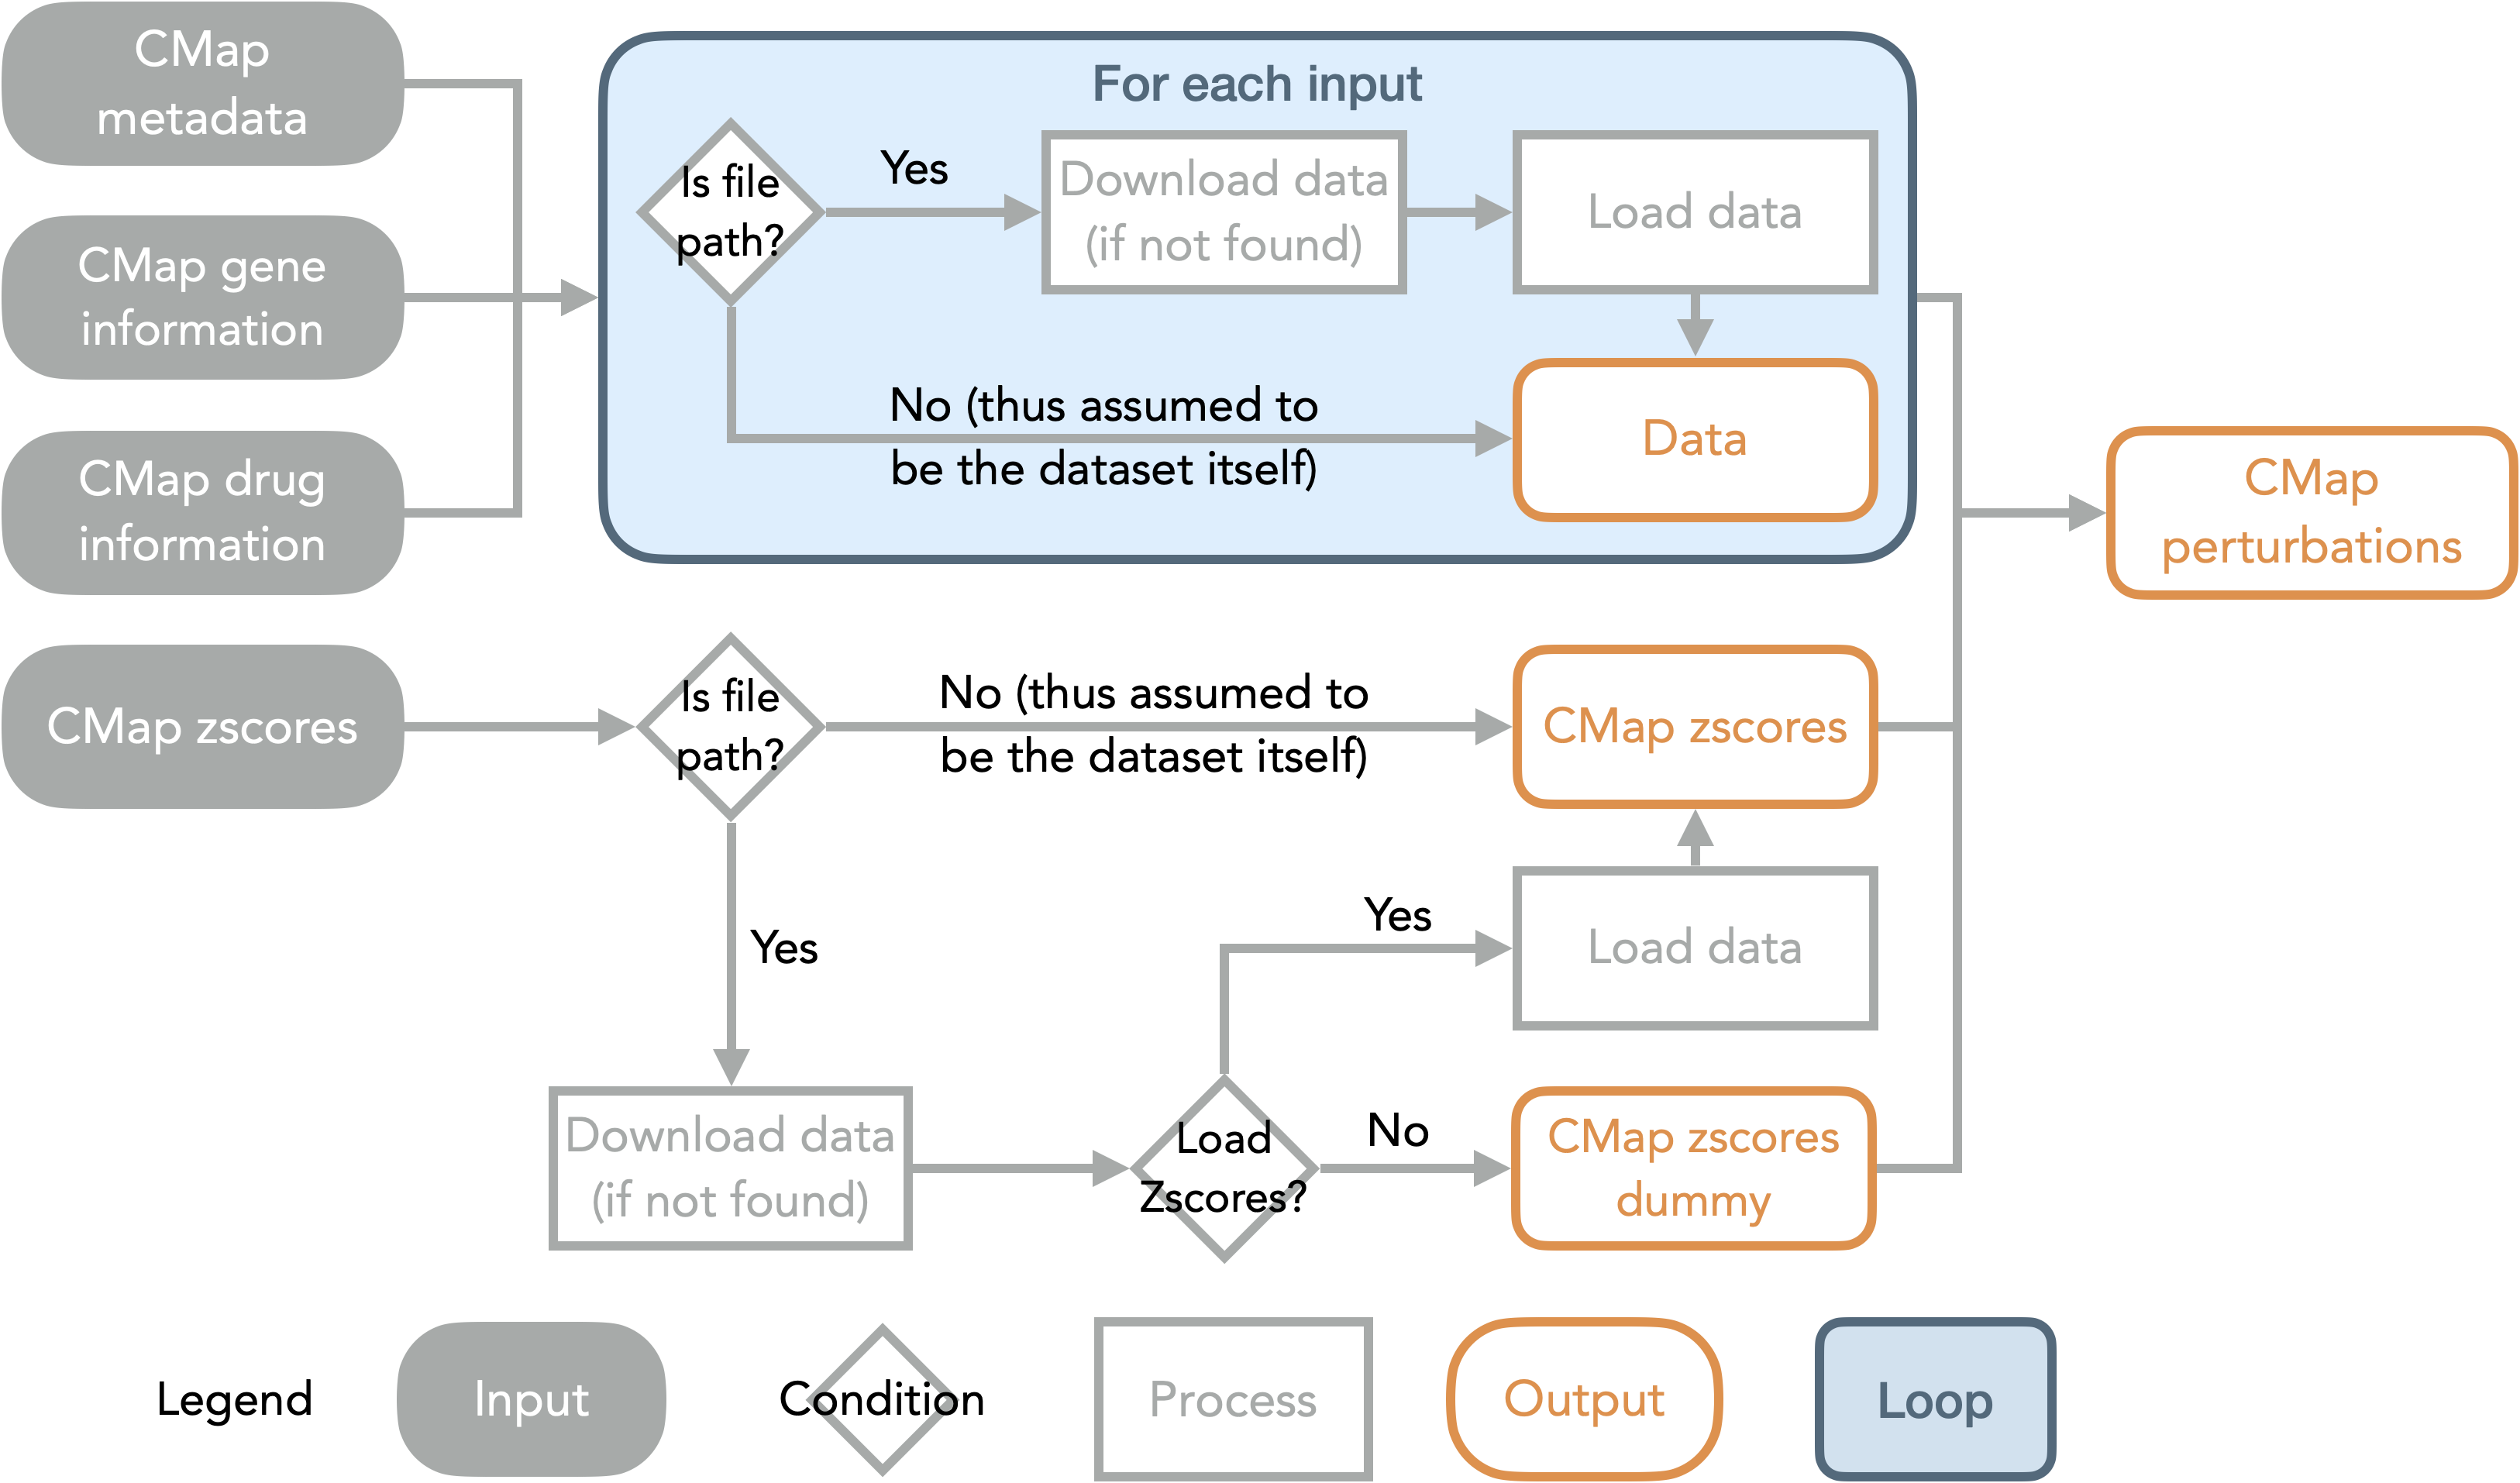
\includegraphics[width=.8\textwidth]{images/ctrap/cmap-perturbations}
  \centering
  \caption[Loading data from CMap perturbations]{\textbf{Loading data from CMap perturbations.} Input arguments support either the data itself (as data frames) or their respective file path. If the file path directs to a non-existing file,  data is first downloaded and then saved to the given file path. To avoid high memory usage, CMap perturbations' z-scores of differential expression profiles (CMap zscores) are not loaded into memory when a file path is given. Instead, only metadata are loaded into a \emph{dummy} object that can be subset as a normal R object for downstream analyses.}
  \label{fig:ctrap-cmap-perturbations}
\end{figure}

CMap perturbations can be categorised into gene knockdown, gene over-expression and compounds. In cTRAP, available perturbation types and respective conditions can be enquired using the function \texttt{getCMapConditions()} that will download CMap perturbation metadata. Afterwards, the function \texttt{filterCMapMetadata()} allows to filter the metadata based on selected perturbations types, cell lines, dosages and time points, allowing to specifically load only the desired data in downstream analyses. This information is passed to \texttt{prepareCMapPerturbations()} to download (if file is not found) and process CMap differential expression profiles z-scores (GCTX file) and gene and compound information (\shortref{fig:ctrap-cmap-perturbations}). Given that the GCTX file size is around 21GB, we recommend to download the file directly from GEO GSE92742’s Level 5 data link (\sloppy{\small{\url{ftp://ftp.ncbi.nlm.nih.gov/geo/series/GSE92nnn/GSE92742/suppl/GSE92742_Broad_LINCS_Level5_COMPZ.MODZ_n473647x12328.gctx.gz}}}).

After comparing differential expression z-scores from select CMap perturbations against user-provided differential expression results, \texttt{rankSimilarPerturbations()} returns a table with ranked CMap perturbations and their respective correlation coefficients and GSEA scores. Lower ranks indicate perturbations whose differential expression profiles are more similar to the user-provided data, i.e. CMap perturbations that potentially mimic the user-provided transcriptomic changes, whereas higher ranks define perturbations that may revert those changes.

To rank CMap perturbations, cTRAP performs Spearman's and Pearson's correlations between the user-provided statistics for differential expression and values from CMap perturbations, and calculates a GSEA-based score (all three methods are run by default). For each method, the similarity scores are averaged across multiple cell lines for the same conditions (when available) and those averages are then used to rank CMap perturbations. By default, results for individual cell lines are provided for informative purposes (e.g. to check the heterogeneity of response across cell lines) but not used when ranking. The different ranking scores are combined via the rank product, ultimately used to sort the CMap perturbations. % rank product not properly explained

The GSEA-based score is calculated via the following steps:

\begin{enumerate}
	\item Sort genes from the user-provided differential expression statistics;
	\item Define the top 150 (by default) and bottom 150 (by default) genes as two sets
	\item For each CMap perturbation, sort genes by their differential expression z-scores and calculate the Weighted Connectivity Score (WTCS) \cite{subramanian:2017ul} based on the GSEA enrichment scores for the two sets.
\end{enumerate}

As an example, for a CMap perturbation with a similar differential expression profile to user’s input, we expect to find higher enrichment of the top gene set in the most up-regulated genes and higher enrichment of the bottom gene set in the most down-regulated genes.

To minimise peak RAM usage, \texttt{prepareCMapPerturbations()} downloads the GCTX file (a customised HDF5 file) for the CMap’s perturbation differential expression z-scores (if not previously downloaded) and returns its path without loading the file content itself, creating a \emph{dummy} object that only stores its file path, perturbation names, gene symbols and other associated metadata (\shortref{fig:ctrap-cmap-perturbations}). Based on the file path of this \emph{dummy} object (that can be subset like a normal R object), \texttt{rankSimilarPerturbations()} loads a $\le$ 1 GiB chunk\footnote{The default 1 GiB ($1024^3$ bytes) allows loading chunks of around 10000 columns and 14000 rows ($10000 \times 14000 \times 8 \textrm{ bytes} / 1024^3 = 1.04 \textrm{ GiB}$). CMap's GCTX file has around 14000 rows (genes).}, compares its differential expression z-score values against user-provided data and repeats the analysis for the next chunk (\shortref{fig:ctrap-analyses}). For each chunk, multithreaded support for Linux and macOS can be enabled per comparison method via \texttt{parallel::mclapply()}\footnote{\texttt{mclapply()} parallelises tasks via forking where multiple child processes are spawned and share their parent's memory. Forking is unavailable in Windows and its alternatives were deemed unsatisfactory, given that they copy 1GiB chunks per thread, significantly slowing down runtime.}, enabled by setting the number of threads to 2 or higher.

\begin{figure}[!h]
  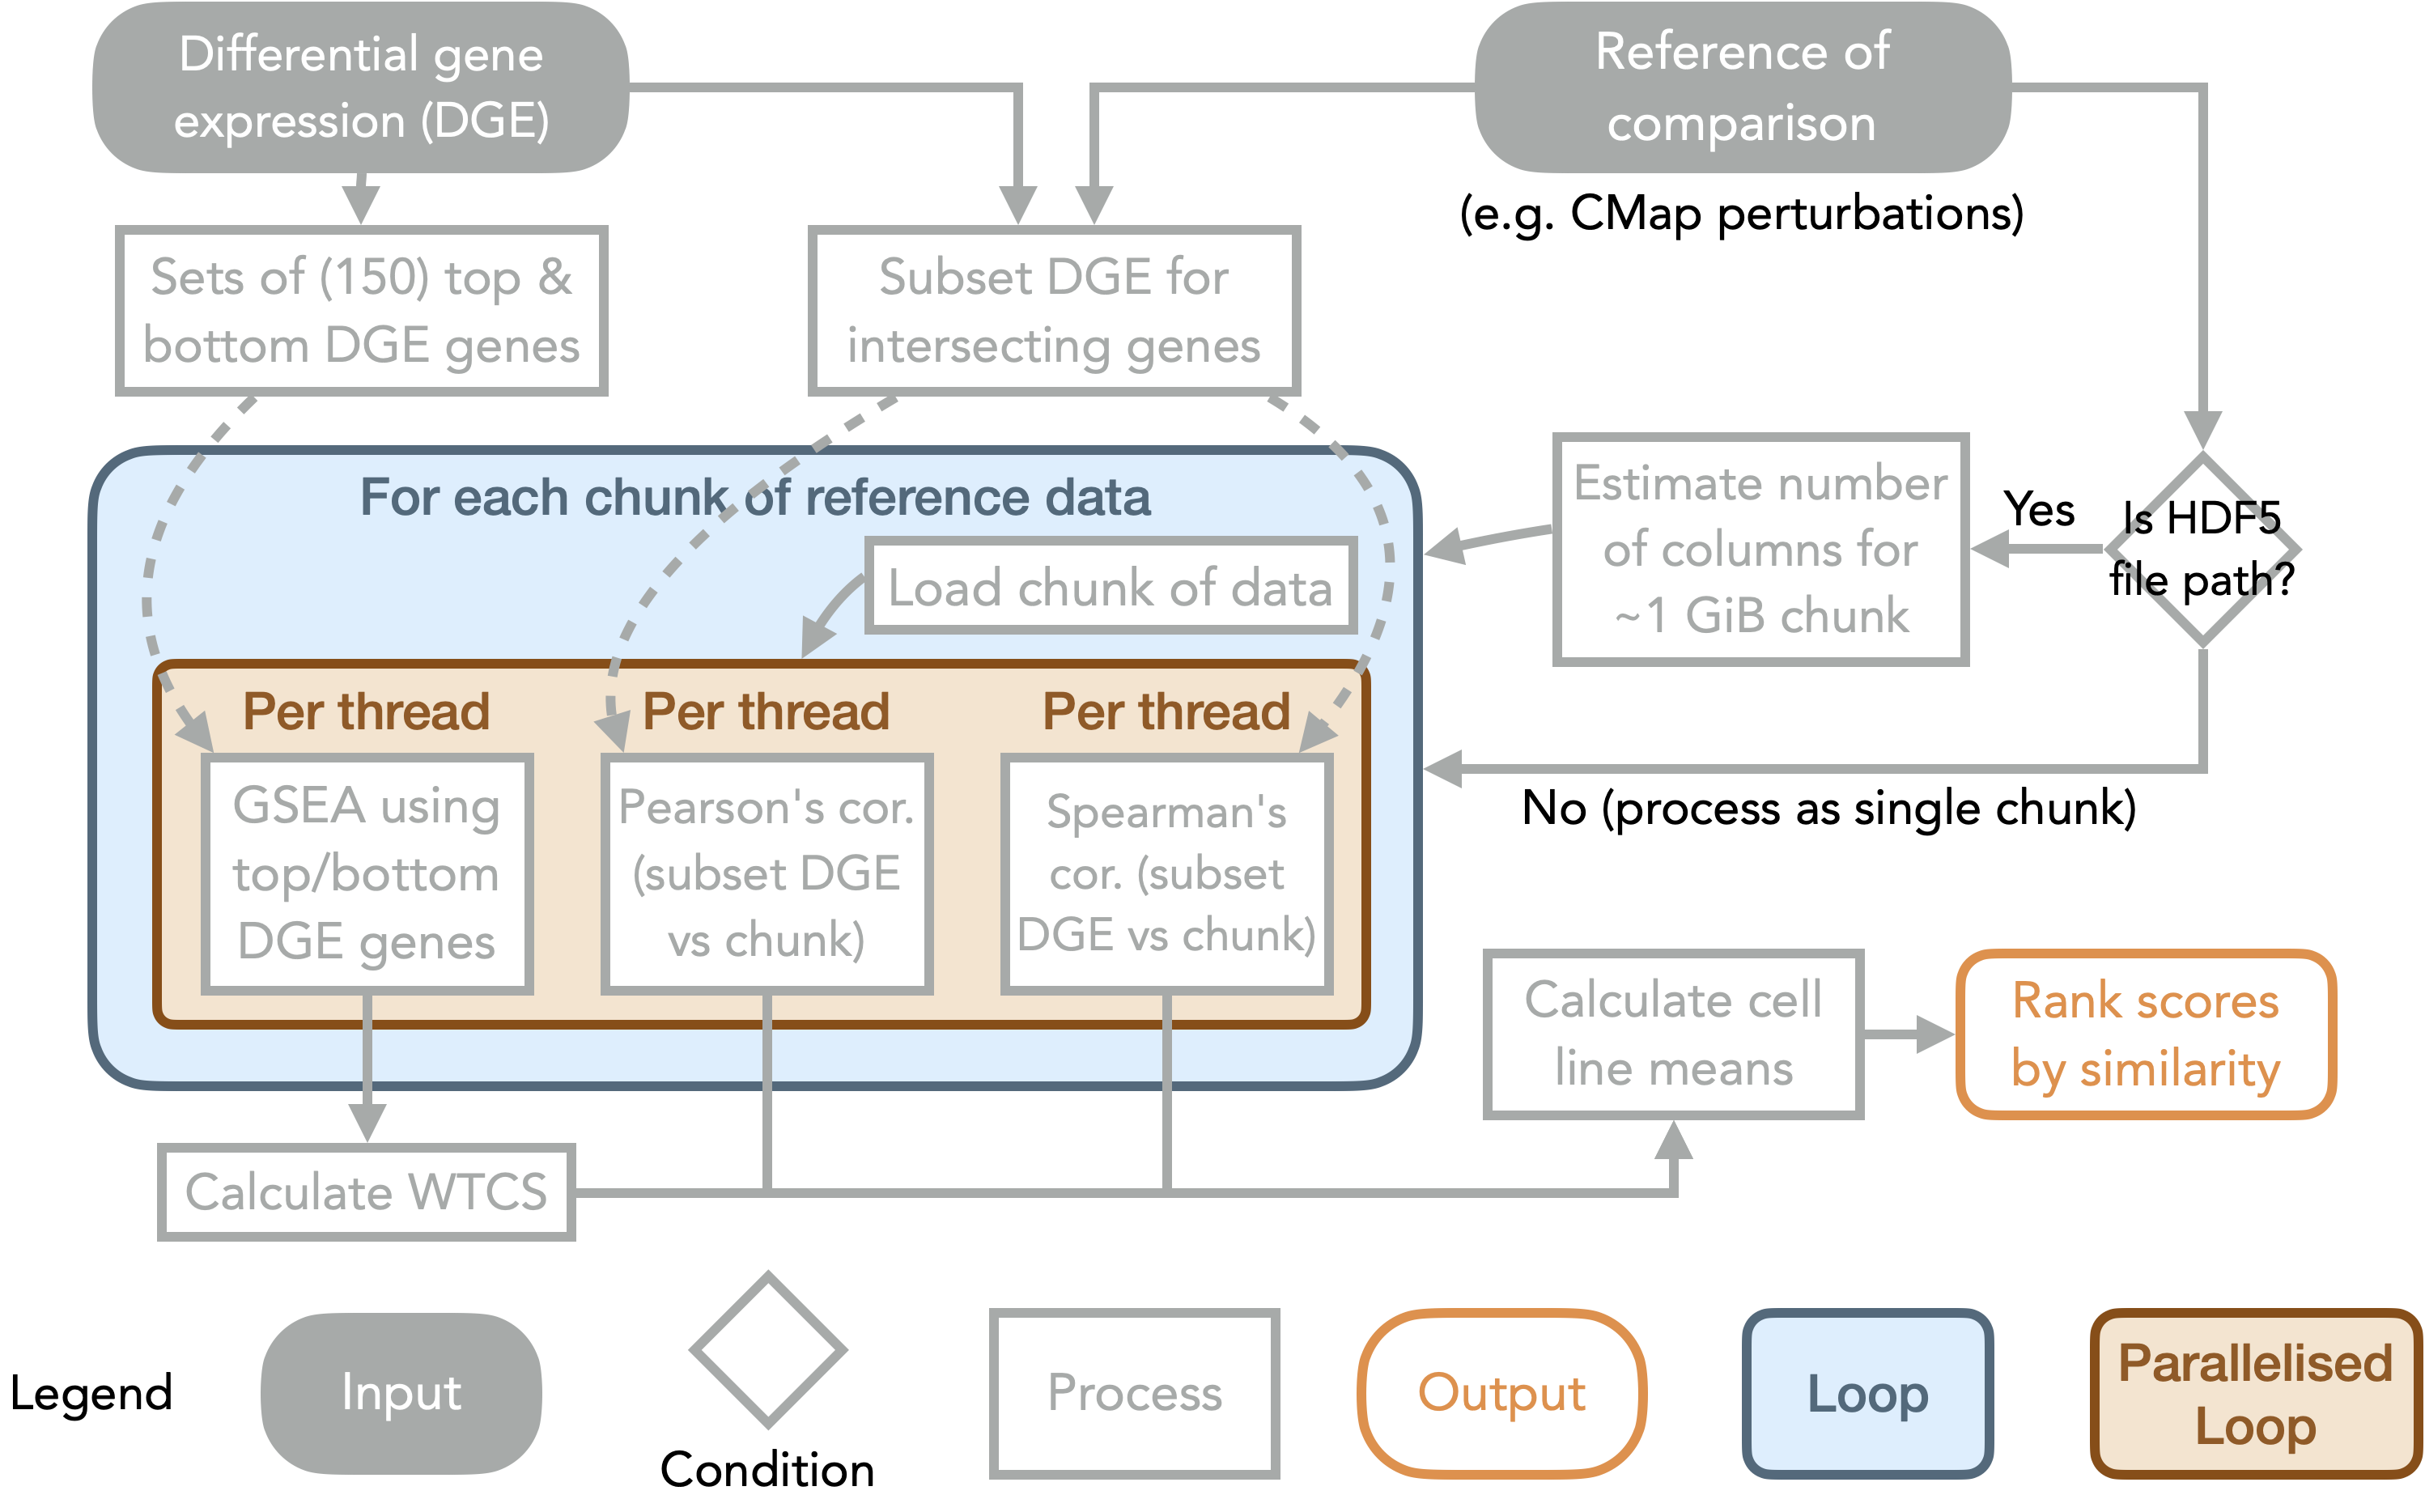
\includegraphics[width=.8\textwidth]{images/ctrap/analysis}
  \centering
  \caption[cTRAP similarity analysis]{\textbf{cTRAP similarity analysis.} User-provided differential gene expression is compared against a reference (e.g. differential expression z-scores of CMap perturbations) and ranked by similarity. If the reference of comparison is a HDF5 file path, the file is processed in 1GiB chunks to minimise peak memory usage. These analyses support multiple threads in Linux and macOS.}
  \label{fig:ctrap-analyses}
\end{figure}

The ranked list from \texttt{rankSimilarPerturbations()} can be plotted using \texttt{plot()}, showing a list of all results ordered by a given score or either a scatterplot or GSEA plot for a predicted targeting drug.

\subsection{Prediction of targeting drugs}

Gene expression and drug activity data across multiple cell lines are available from NCI-60 \cite{shoemaker:2006wi}, Cancer Therapeutics Response Portal (CTRP) 2.1 \cite{seashore-ludlow:2015ws} and Genomics of Drug Sensitivity in Cancer (GDSC) 7 \cite{yang:2012vk}. For each source, the internal function \texttt{prepareExpressionDrugSensitivityAssociation()} performs the following steps:

\begin{enumerate}
	\item Download all the necessary data depending on given source;
	\item Perform Spearman’s correlation (by default) between the expression of each gene against the sensitivity of intersecting cell lines to each drug;
	\item Generate a matrix with the correlation coefficients per gene and drug; and
	\item Prepare metadata for downstream analyses, including gene, compound and cell line information from each source.
\end{enumerate}

A higher correlation coefficient for a given gene and drug suggests a gene whose higher expression is associated with higher drug sensitivity across multiple cell lines. As this process can take multiple hours to finish for all sources, the resulting objects were stored online for each aforementioned source and can be listed with \texttt{listExpressionDrugSensitivityAssociation()} and downloaded and loaded into R using \texttt{loadExpressionDrugSensitivityAssociation()}.

To identify compounds that could target the phenotype associated with specific differential expression profiles, we use \texttt{predictTargetingDrugs()} with those profiles and a correlation matrix of gene expression and drug sensitivity as input. The correlation coefficients between gene expression and drug sensitivity for each drug are compared against user-provided differential expression results by Spearman’s and Pearson’s correlation and GSEA-based scores (as performed when ranking CMap perturbations, results from comparison methods are ranked and then those rankings are finally used to calculate the rank product’s rank). \texttt{predictTargetingDrugs()} returns a table with ranked predicted targeting drugs and their respective correlation coefficients and GSEA scores (\shortref{fig:ctrap-analyses}). A lower rank comprise drugs that may target phenotypes similar to the user-provided differential expression profile.

The resulting object can be plotted with \texttt{plot()}, showing a list of all results ordered by a given score or either a scatterplot or GSEA plot for a predicted targeting drug.

The function \texttt{plotTargetingDrugsVSsimilarPerturbations()} compares the results from predicted targeting drugs and CMap perturbations that may mimic or revert the observed phenotype. For the available compound identifiers in the metadata pertaining from the different datasets (e.g. compound name, Broad ID, PubChem CID and SMILES), the function will automatically select the identifiers with higher number of matching values between the two datasets, unless the identifiers are explicitly defined by the user. A scatterplot is then returned using, by default, the rank product’s rank of targeting drugs in one axis and the rank product’s rank of similar perturbations in the other.

\subsection{Drug descriptor set enrichment analysis}

Juan Carlos, a former member of the lab, computed drug descriptors (e.g. molecular weight and number of aromatic rings) for compounds from CMap and NCI-60 based on their three-dimensional (3D) and two-dimensional (2D) characteristics. These descriptors were uploaded to \alink{compbio.imm.medicina.ulisboa.pt/public/cTRAP/} and the resulting files can be automatically downloaded and processed to R using \texttt{loadDrugDescriptors()}.

\texttt{prepareDrugSets()} allows to create sets of descriptors. By default, the function creates a maximum of 15 sets per drug descriptor. For each alphanumeric descriptor, one set is created per unique value of that descriptor. Alphanumeric descriptors containing more than 15 unique values (by default) will be discarded. For numerical descriptors, \texttt{prepareDrugSets()} internally uses the \texttt{binr::bins()} function to create evenly-distributed bins of drug descriptors, where each set contains a minimum number of points equal to the number of non-missing values divided by the number of maximum sets (15 by default) divided by a constant (5 by default).

The function \texttt{analyseDrugSetEnrichment()} analyses the enrichment of the created drug descriptor sets in a named numeric vector or an object returned from \texttt{rankSimilarPerturbations()} – only if run against CMap compound perturbations – or \texttt{predictTargetingDrugs()}. The GSEA-based enrichment analysis is internally performed using \texttt{fgsea::fgsea()}.

The resulting object can be plotted with \texttt{plot()}, showing a list of all results ordered by a given score or either a scatterplot or GSEA plot for a predicted targeting drug.

\subsection{Time and memory benchmarking}

We measured elapsed time using R’s \texttt{Sys.time()} immediately before and after ranking similar CMap perturbations, predicting targeting drugs (using NCI60 expression and drug sensitivity association, the most time-consuming option) and performing drug set enrichment analysis using cTRAP 1.8.1 (296f9b21). As input, we used the t-statistics for the differential expression between EIF4G1 knockdown versus control based on ENCODE gene expression data from cell line HepG2 (the \texttt{diffExprStat} object in the cTRAP package).

We measured the heap memory usage of cTRAP 1.8.1 (296f9b21) across time by running R 4.0.3 in debug mode with the heaptrack 1.0.0 profiler. heaptrack tracks and logs all calls to the core memory allocation functions via \verb|LD_PRELOAD| and respective backtraces. For R to work properly with heaptrack, the file \path{/usr/bin/R} was edited -- all lines of the last \emph{if} statement were commented out, except for:

\begin{lstlisting}[language=bash,numbers=none]
exec ${debugger} ${debugger_args} "${R_binary}" ${args} "${@}"
\end{lstlisting}

Afterwards, we benchmarked R scripts running cTRAP with:

\begin{lstlisting}[language=bash,numbers=none]
R -d heaptrack -f ${cTRAP_Rscript} --args ${cTRAP_Rscript_args}
\end{lstlisting}

All benchmarks were run in a workstation running Ubuntu 18.04.5 LTS with 768 GB of RAM memory and 72 cores (Intel Xeon Gold 6254 CPU @ 3.10GHz). The benchmarked cTRAP scripts are publicly available in cTRAP's GitHub repository: \alink{github.com/nuno-agostinho/cTRAP/tree/master/dev/benchmark}

\subsection{Continuous integration}

Akin to psichomics (\fullref{subsec:psichomics-ci}), GitHub Actions are used with cTRAP to update its Docker images in Docker Hub (\dockerlink{nunoagostinho/ctrap}) and GitHub (\alink{github.com/nuno-agostinho/cTRAP}); update website documentation via \texttt{roxygen} \cite{wickham:2021wt} and \texttt{pkgdown} \cite{wickham:2021wj}; and check for errors and warnings when building cTRAP in Windows, macOS and Linux.

\section{Results}

cTRAP's web app is available at \alink{compbio.imm.medicina.ulisboa.pt/cTRAP}. Alternatively, users can install cTRAP in their own computers, allowing them to use local computing resources. Similarly to psichomics, cTRAP offers both graphical and command-line interfaces. Although most features are common to both interfaces, we recommend less experienced users to opt for the Shiny-based graphical interfaces.

\subsection{Case study}

For this case study, we used RNA-seq data from EIF4G1 shRNA knockdown experiments in HepG2 cell line from the ENCODE project. The RNA-seq processed data (gene quantifications from RSEM method) for the EIF4G1 knock-down and respective controls (two replicates each) was automatically downloaded by cTRAP.

\subsubsection{Differential gene expression analysis of ENCODE RNA-seq data}

Gene expression data (read counts) were quantile-normalized using voom, followed by differential expression analysis performed using \texttt{limma} \cite{ritchie:2015tm}. We used the respective t-statistic as our metric of differential expression to compare with CMap’s gene knock-down perturbations in the same cell line (HepG2)\footnote{This comparison could also be done to perturbations in a different cell line (or in all cell lines using the average result across cell lines).}.

% To summarise conditions and check available data in CMap, we can use the following commands to download CMap metadata:

Afterwards, we filtered the metadata to CMap gene knockdown perturbations in HepG2 and loaded associated gene information and differential gene expression data based on the given filename. The differential gene expression z-scores from CMap were also loaded for small molecule perturbations.

Differential gene expression data for each CMap perturbation are available in normalised z-score values \cite{subramanian:2017ul}.

\subsubsection{Comparison with CMap perturbations}

The \texttt{rankSimilarPerturbations()} function compares the differential expression metric (the t-statistic, in this case) against the CMap perturbations’ z-scores using the available methods:

\begin{itemize}
    \item Spearman’s correlation
    \item Pearson’s correlation
    \item Gene Set Enrichment Analysis (GSEA), where the most up- and down-regulated n genes from the user’s differential expression profile are used as gene sets (by default, $n = 150$ genes)
\end{itemize}

The output table contains the results of the comparison with each perturbation tested, including the test statistics (Spearman’s correlation coefficient, Pearson’s correlation coefficient and/or GSEA score), the respective p-value and the Benjamini-Hochberg-adjusted p-value (for correlation statistics only). When performing multiple methods, the rank product’s rank will be included to summarise other method’s rankings.

The Gene Set Enrichment Analysis (GSEA) score is based on the Weighted Connectivity Score (WTCS), a composite and bi-directional version of the weighted Kolmogorov-Smirnov enrichment statistic (ES) \cite{subramanian:2017ul}. To calculate the GSEA score, GSEA is run for the most up- and down-regulated genes from the user’s differential expression profile. The GSEA score is the mean between EStop and ESbottom (however, if EStop and ESbottom have the same sign, the GSEA score is 0).

If a perturbation has a similar differential expression profile to our data (higher GSEA score), we expect to see the most up-regulated (down-regulated) genes in the perturbation enriched in the top (bottom) n differentially expressed genes from our data.

To analyse the relationship between the user-provided differential expression profile with that associated with a specific perturbation, scatter plots (for Spearman and Pearson analyses) and GSEA plots are available.

For instance, let’s plot the relationship between EIF4G1 shRNA knockdown from ENCODE with the CMap knockdown perturbations.

\subsubsection{Predicted targeting drugs}

Compounds that target the phenotypes associated with the user-provided differential expression profile can be inferred by comparing against gene expression and drug sensitivity associations. The gene expression and drug sensitivity datasets derived from the following sources were correlated using Spearman’s correlation across the available cell lines.

\begin{table}[!ht]
\centering
\parnotereset
\small
\caption[Drug sensitivity datasets statistics]{\textbf{Drug sensitivity datasets statistics.} Number of screened compounds and human cancer cell lines per source.}
\label{tab:drug-sensitivity-datasets}
\begin{tabularx}{.47\textwidth}{ l r r }
\toprule
\textbf{Source}   & \textbf{Compounds} & \textbf{Cell lines} \\
\midrule
NCI60             &                   Over 100 000 & 60 \\
GDSC 7            &                            481 & 860 \\
CTRP 2.1          &                            138 & Around 700 \\
\bottomrule
\end{tabularx}
\parnotes
\end{table}

To use an expression and drug sensitivity association based on CTRP 2.1 (GDSC 7 and NCI60 could be used instead) to infer targeting drugs for the user’s differential expression profile.

Compounds are ranked by their relative targeting potential based on the input differential expression profile (i.e. the 1st-ranked compound has higher targeting potential than the 2nd-ranked one).

Candidate targeting drugs were plotted against the similarity ranking of their perturbations towards the user’s differential expression profile. Note that the highlighted values are the same compounds for the following plots annotated with their name, gene target and mechanism of action (MOA), respectively.

\subsubsection{Molecular descriptor enrichment analysis}

Using our candidate targeting drugs, we analysed the enrichment of 2D and 3D molecular descriptors based on CMap and NCI60 compounds. Our list of targeting drugs is particularly enriched in specific drug descriptors that allows us think about the relevance of these descriptors for targeting a phenotype of interest.

\subsection{Time and memory optimisation}

Show benchmarks.

\subsection{Graphical interface}

Recently, cTRAP was updated to include a visual interface to assist users interactively perform most cTRAP features via the web browser. The graphical interface was modularly built and exposed via 5 functions that work harmoniously with R code:

\begin{itemize}
	\item \texttt{launchDiffExprLoader()} to load differential expression data. Returns a differential expression object that can be used in cTRAP analyses.
	\item \texttt{launchCMapDataLoader()} to explore and load CMap data by type of perturbation, cell types, time points and dosages. Returns filtered CMap data based on the user's selection.
	\item \texttt{launchMetadataViewer()} to check metadata of given cTRAP objects.
	\item \texttt{launchResultPlotter()} to view and plot cTRAP results given as input.
	\item \texttt{launchDrugSetEnrichmentAnalyser()} to analyse drug set enrichment and visualize respective results.
\end{itemize}

Like usual R functions, these graphical interfaces functions accept input arguments and may return output, thus allowing to intertwine them with R code and to easily reproduce cTRAP analyses (\shortref{lst:cTRAP-graphical}).

\begin{lstlisting}[caption=Calling cTRAP's graphical interface functions in an R script.,label={lst:cTRAP-graphical},language=R,morekeywords={include, launchDiffExprLoader},keywordstyle=\bfseries]
# Launch differential expression loading interface to select knockdown
# data from ENCODE (pre-filtered for HepG2 cell line and EIF4G1 gene)
diffExpr <- launchDiffExprLoader(cellLine="HepG2", gene="EIF4G1")

# After filter selection, launchDiffExprLoader() does the following:
# 1. Download ENCODE's HepG2 data for EIF4G1 knockdown and controls
# 2. Perform DGE between EIF4G1 knockdown vs. control
# 3. Return resulting t-statistics by gene

# Load CMap knockdown data in HepG2
cmapKD <- launchCMapDataLoader(
    cellLine="HepG2",
    perturbationType="Consensus signature from shRNAs targeting the same gene")
# Load CMap compound data in HepG2
cmapCompounds <- launchCMapDataLoader(cellLine="HepG2",
                                      perturbationType="Compound")
# Load all CMap data in HepG2
cmapPerts <- launchCMapDataLoader(cellLine="HepG2")

# View metadata of all resulting CMap data objects
launchMetadataViewer(cmapKD, cmapCompounds, cmapPerts)

# Rank similar perturbations -----------------------------------------
compareKD        <- rankSimilarPerturbations(diffExpr, cmapKD)
compareCompounds <- rankSimilarPerturbations(diffExpr, cmapCompounds)
comparePerts     <- rankSimilarPerturbations(diffExpr, cmapPerts)

launchResultPlotter(compareCompounds, compareKD, comparePerts)

# Predict targeting drugs --------------------------------------------
listExpressionDrugSensitivityAssociation()
assocMatrix <- listExpressionDrugSensitivityAssociation()[[1]]
assoc       <- loadExpressionDrugSensitivityAssociation(assocMatrix)
predicted   <- predictTargetingDrugs(diffExpr, assoc)
launchResultPlotter(predicted)

# Plot targeting drugs vs similar perturbations ----------------------
launchResultPlotter(predicted, compareCompounds)

# Analyse drug set enrichment ----------------------------------------
descriptors <- loadDrugDescriptors("NCI60", "3D")
drugSets    <- prepareDrugSets(descriptors)

launchDrugSetEnrichmentAnalyser(drugSets, compareCompounds)
launchDrugSetEnrichmentAnalyser(drugSets, predicted)
\end{lstlisting}

cTRAP is also available online\footnote{More information in \fullref{chap:app-server}.} with a comprehensive interface that provides most aforementioned features in a single app via a sixth function: \texttt{cTRAP()}. Such a strategy lead to this question: how to deal with long-running tasks? The way R/Shiny is built, an entire cTRAP session would be consuming useful resources during the cTRAP analyses, but this would not properly scale for multiple users using heavy memory resources simultaneously. To avoid this, long-running tasks are managed via job queues depending on available resources and run in the background. But this also means that the system must allow users to get their results back once they finish calculating. And thus the idea of user sessions was born.

\subsubsection{User sessions}
\label{sec:ctrap-web}

\begin{wrapfigure}{r}{.4\textwidth}
  \vspace{-2\intextsep}
  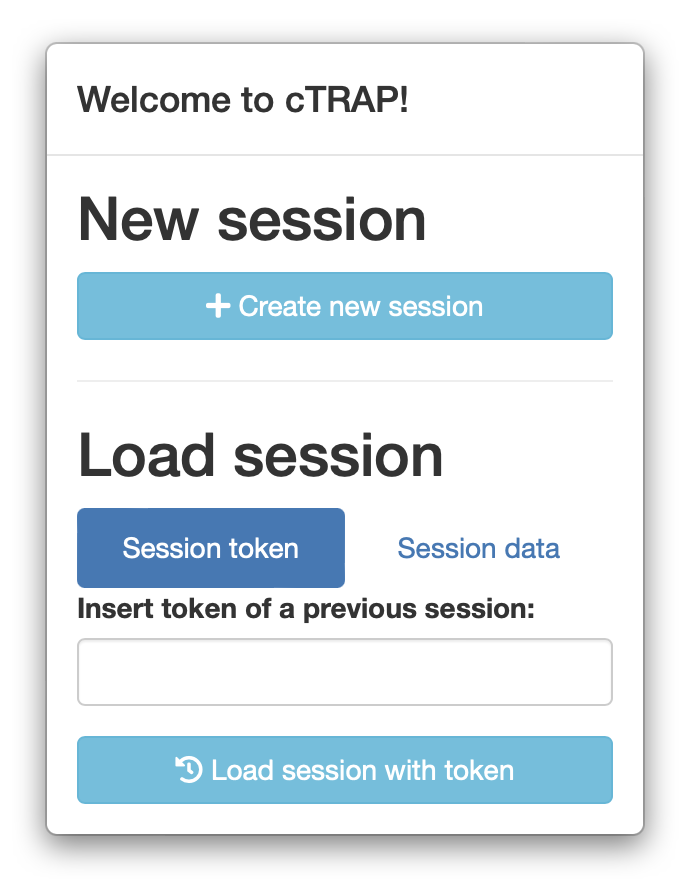
\includegraphics[width=\linewidth]{images/ctrap/welcome}
  \caption[Welcome screen modal]{\textbf{Welcome modal.}}
  \vspace{-1\intextsep}
  \label{fig:ctrap-welcome}
\end{wrapfigure}

Session data are saved in folders named after a random alphanumeric string (token) that uniquely identifies each session and can be downloaded as RDS files. Given that the downloaded file is a list of all datasets from the user session, users can load these RDS files in any R session and in local instances of cTRAP. Downloading user sessions is encouraged because cTRAP session folders are removed from our server if not accessed in the last 30 days based on the access timestamp\footnote{In Linux, the access timestamp (\texttt{atime} attribute) for a directory indicates the last time a file within was read/written or its contents were listed.}.

cTRAP visitors are greeted with a welcome screen that allows them to create a new session or restore previous ones (\autoref{fig:ctrap-welcome}), a dialog that can be opened at any time from the session menu.

% TODO: mention other files in common across cTRAP?
When creating a new session, a unique a token is created. As soon as session-specific data is loaded, a new folder is created in the working directory and named after the session token (\autoref{fig:user-session}). Any updates to the session data are automatically saved to the session folder. To avoid downloading commonly-used files (e.g. the 21GB CMap perturbations z-scores file), an appropriate folder stores data shared across sessions, thus avoiding downloading, storing and processing redundant data.

When restoring a session via a token, cTRAP loads the contents of the folder named after the token located in cTRAP working directory or warns the user if no such folder exists (\autoref{fig:user-session}). In case the user uploads a RDS file of a previous session, cTRAP will load its contents in a new session (\autoref{fig:user-session}).

\begin{figure}[!ht]
  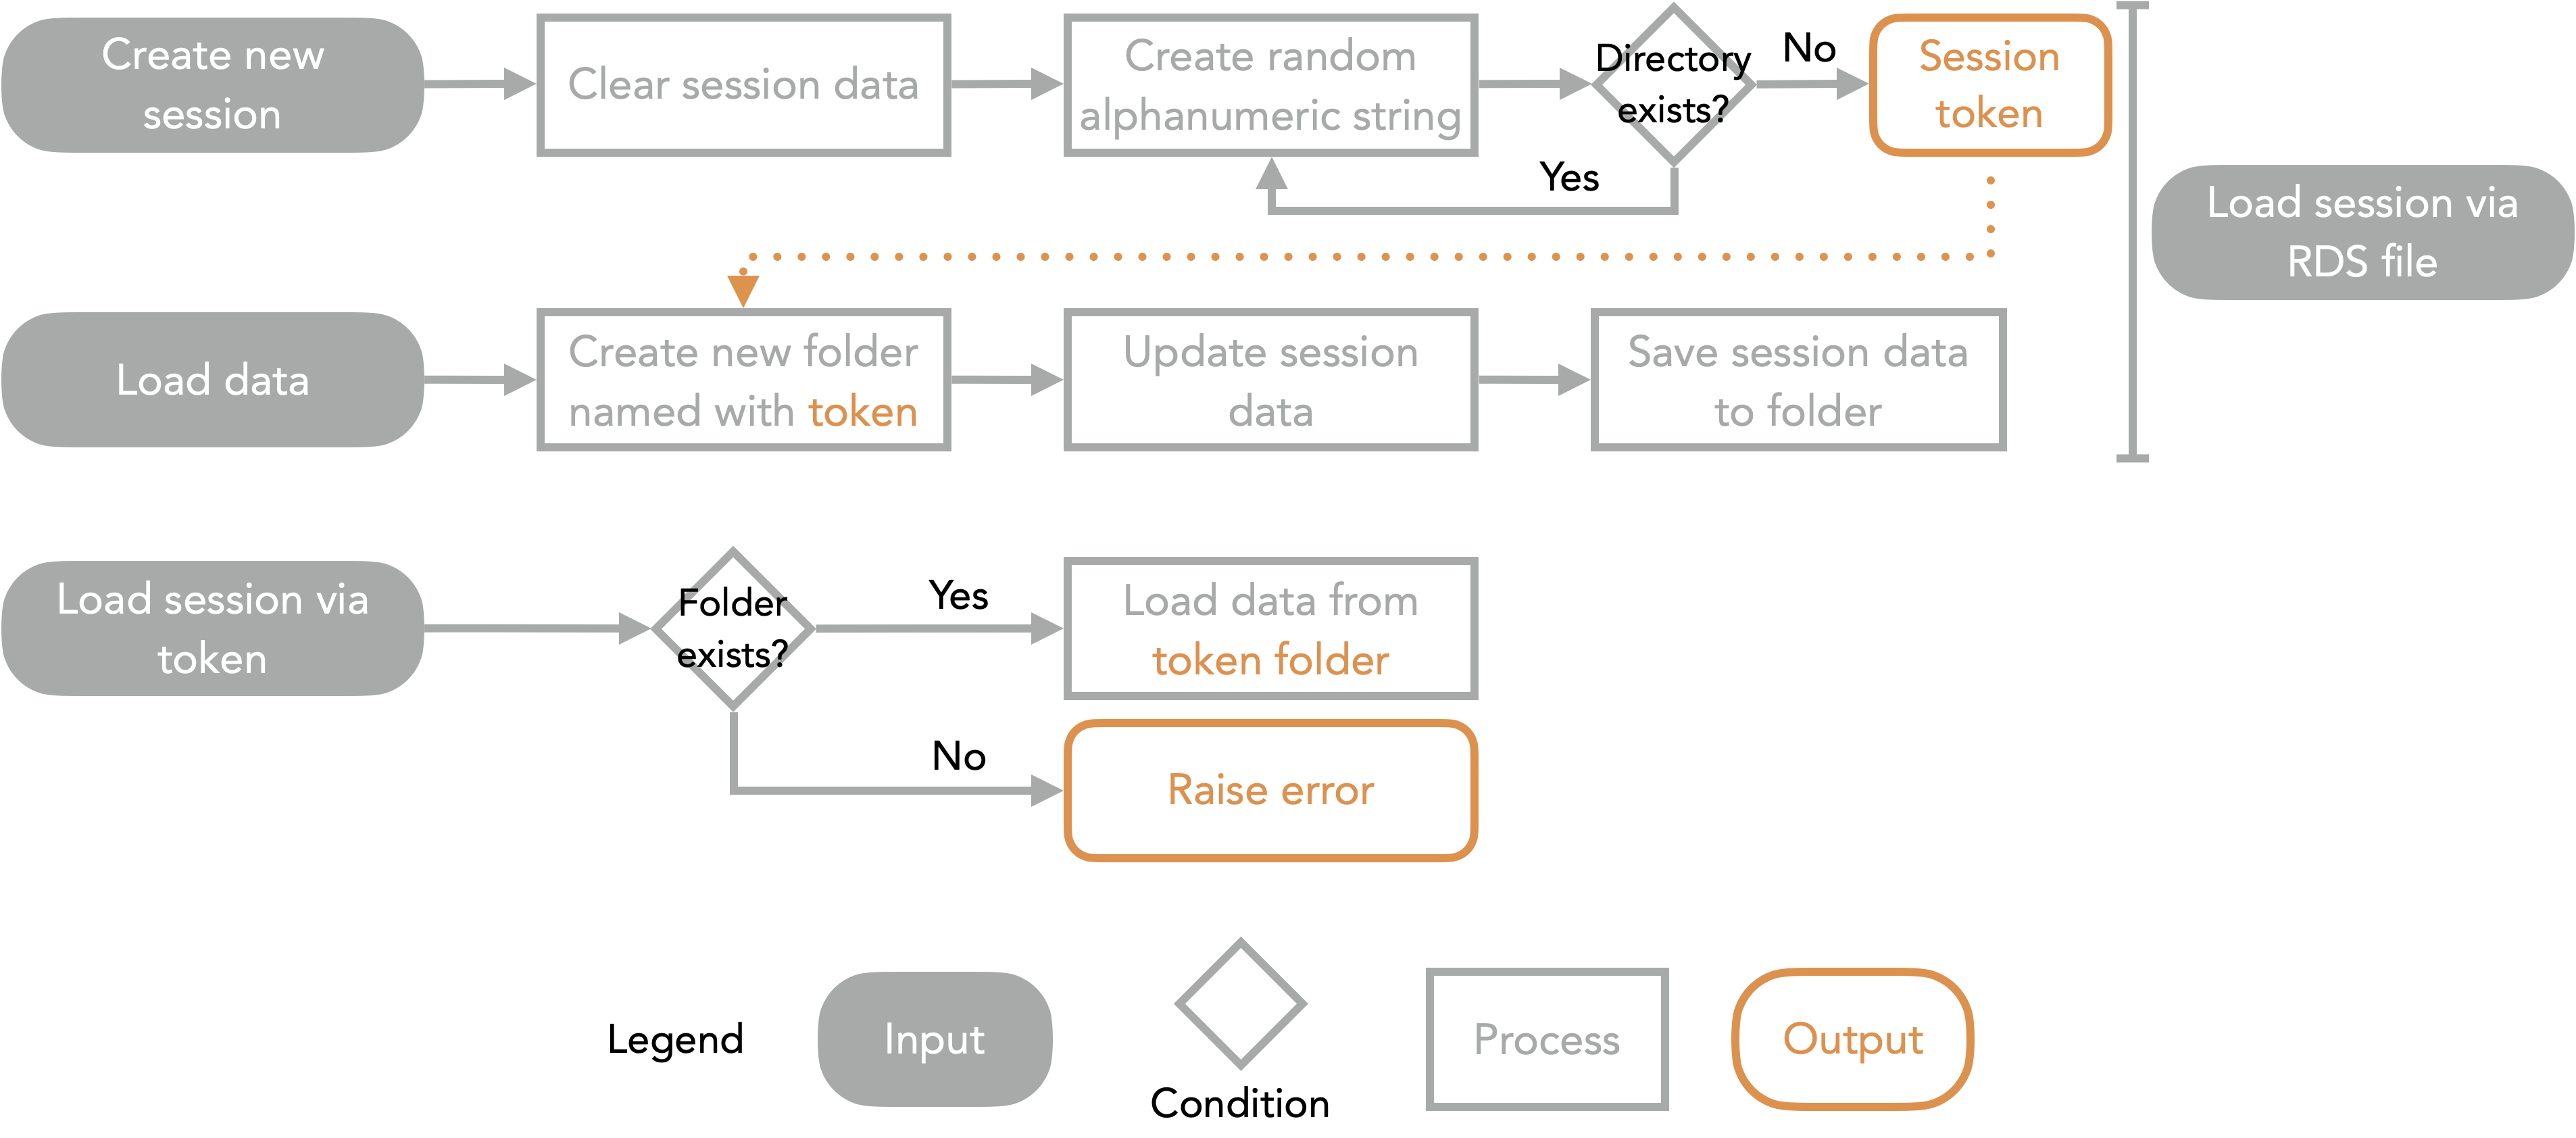
\includegraphics[width=\textwidth]{images/ctrap/user-session}
  \centering
  \caption[User session workflow]{\textbf{User session workflow.} cTRAP allows to create new sessions or load a previous one via a given token or RDS file. When loading session via a RDS file, a new cTRAP session is created before loading the data from RDS file. Sessions can also be loaded using a token if any folder with such token exists in cTRAP's working directory.}
  \label{fig:user-session}
\end{figure}

\subsubsection{Background tasks}
\label{subsec:background-tasks}

When running a Shiny app, the user has to wait for the long-running tasks to finish before the app starts responding to user's commands again. Critically, if cTRAP is shut down, all running processes will stop.

This can be solved by using the R packages \texttt{promises}/\texttt{future} or by manually running another R process in the background. However, these solutions require the Shiny app to be active during the whole process, which can be especially egregious if the R session is consuming many computing resources, disallowing other apps or users to take advantage of those resources until the whole session is terminated.

What are the best options to run large tasks in the background? In Lobo, iMM's computing cluster, we use a job scheduler for that function: SLURM. However, SLURM is too complex to install -- I was not able to create a working prototype of SLURM for a single machine using Docker or otherwise. Anyway, we can use these light-weight alternatives instead:

\begin{itemize}
	\item \textbf{Celery}, a task queue manager written in Python; and
	\item \textbf{Flower}, a monitoring app that provides an HTTP API and graphical interface to manage Celery jobs.
\end{itemize}

Celery requires a \texttt{tasks.py} file with the code of the jobs to run. Given that Celery will run cTRAP functions, cTRAP must be installed alongside Celery. Moreover, as we intend to run R code, one of the Celery tasks is to run R via Python's module \texttt{subprocess} to spawn new processes with the \texttt{Rscript} command (\shortref{lst:tasks.py}).

\begin{lstlisting}[language=python,caption=An example \texttt{tasks.py} file to run R commands or Rscript files via Celery.,label={lst:tasks.py},morekeywords={import},keywordstyle=\bfseries]{tasks.py}
import os, time
from datetime import datetime
from subprocess import run, PIPE

# Celery configuration
from celery import Celery
os.environ.setdefault('C_FORCE_ROOT', 'true')
app = Celery(
    "tasks",
    broker=os.environ.get('CELERY_BROKER_URL', 'redis://redis'),
    backend=os.environ.get('CELERY_RESULT_BACKEND', 'redis://redis'))
app.conf.CELERY_WORKER_SEND_TASK_EVENTS = True

# Runs R command and returns output
#   - Use cat(), e.g. 'cat(2+2)', to capture output as a job result
#   - Errors will result in a task state of FAILURE
def execR(cmd):
    return run(cmd, check=True, stdout=PIPE, text=True).stdout

# Run a given R expression as a Celery job
@app.task
def R(cmd): return execR(["Rscript", "-e", cmd])

# Run a given Rscript file as a Celery job
@app.task
def Rscript(cmd): return execR(["Rscript", cmd])

if __name__ == "__main__": app.start()
\end{lstlisting}

Flower can send jobs to Celery via HTTP methods, facilitating the communication between cTRAP and Celery. To assist using Flower in R, I created the R package \texttt{floweRy} (\alink{github.com/nuno-agostinho/floweRy}) that contains wrapper functions for most of its HTTP API functions. Internally, \texttt{floweRy} calls HTTP methods with \texttt{httr} R package, creating dedicated commands that make it easier than using just plain \texttt{httr}, as briefly demonstrated in Listings \shorterref{lst:httr} and \shorterref{lst:floweRy}.

\noindent\begin{minipage}{.48\textwidth}
\begin{lstlisting}[caption=Job submission with \texttt{httr}.,language=R,label={lst:httr}]{httr}
library(httr)
flower <- function(...) paste0(
    "http://localhost:5555", ...)
# Run R command '3 + 4' in Celery
POST(flower("/api/task/apply/tasks.R")), body="3 + 4", encode="json")
# Get status of all Celery tasks
GET(flower("/api/tasks"))
\end{lstlisting}
\end{minipage}\hfill
\begin{minipage}{.48\textwidth}
\begin{lstlisting}[caption=Job submission with \texttt{floweRy}.,language=R,label={lst:floweRy}]{floweRy}
library(floweRy)
options(flowerURL=
    "http://localhost:5555")
# Run R command '3 + 4' in Celery
taskApply("tasks.R", "3 + 4")


# Get status of all Celery tasks
taskList()
\end{lstlisting}
\end{minipage}

cTRAP currently supports ranking similar CMap perturbation and predicting targeting drugs as background processes by submitting jobs to Celery with the exact R commands to run via the \texttt{Rscript} command \cite{r-core-team:2021wf}. The status of background tasks can be monitored by users in the respective cTRAP's user session (\shortref{fig:job-progress})\footnote{Flower also allows to monitor and manage Celery jobs, but its web interface is only accessible in the iMM network (via ethernet cable or VPN). More information in \fullref{sec:background-tasks}.}.

\begin{figure}[!h]
  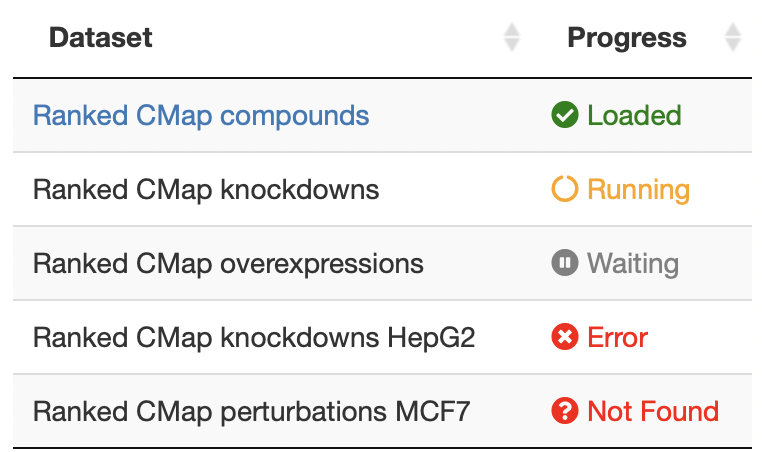
\includegraphics[width=.5\textwidth]{images/ctrap/job-progress}
  \centering
  \caption[Progress of Celery jobs in cTRAP]{\textbf{Progress of Celery jobs in cTRAP.} The job status are updated every 5 seconds. Their status can be: \textcolor{gray}{Waiting} in job queue to start, \textcolor{orange}{Running}, \textcolor{teal}{Loaded}, \textcolor{red}{Error} for unknown failures, and \textcolor{red}{Not Found} if the job results cannot be found (e.g. when re-uploading the same RDS file, the job results were already cleaned-up in the first upload). When a job finishes, a blue link is added to the job name in order to directly access its results in cTRAP.}
  \label{fig:job-progress}
\end{figure}

All Celery jobs are saved as \emph{dummy} objects in cTRAP's user session data, containing the job identifier and metadata from expected results. When the background processes finish, their output is saved into the session folder. If the user is actively using that session in the cTRAP website, the data is automatically loaded -- replacing the previous \emph{dummy} objects -- and the user is informed of such via a notification in cTRAP (\shortref{fig:ctrap-celery}). Otherwise, next time that session is loaded by the user (either via its token or an RDS file), the job for every \emph{dummy} object in the session data is returned if finished.

% TODO: file is removed after its object is loaded: confirm
\begin{figure}[!htb]
  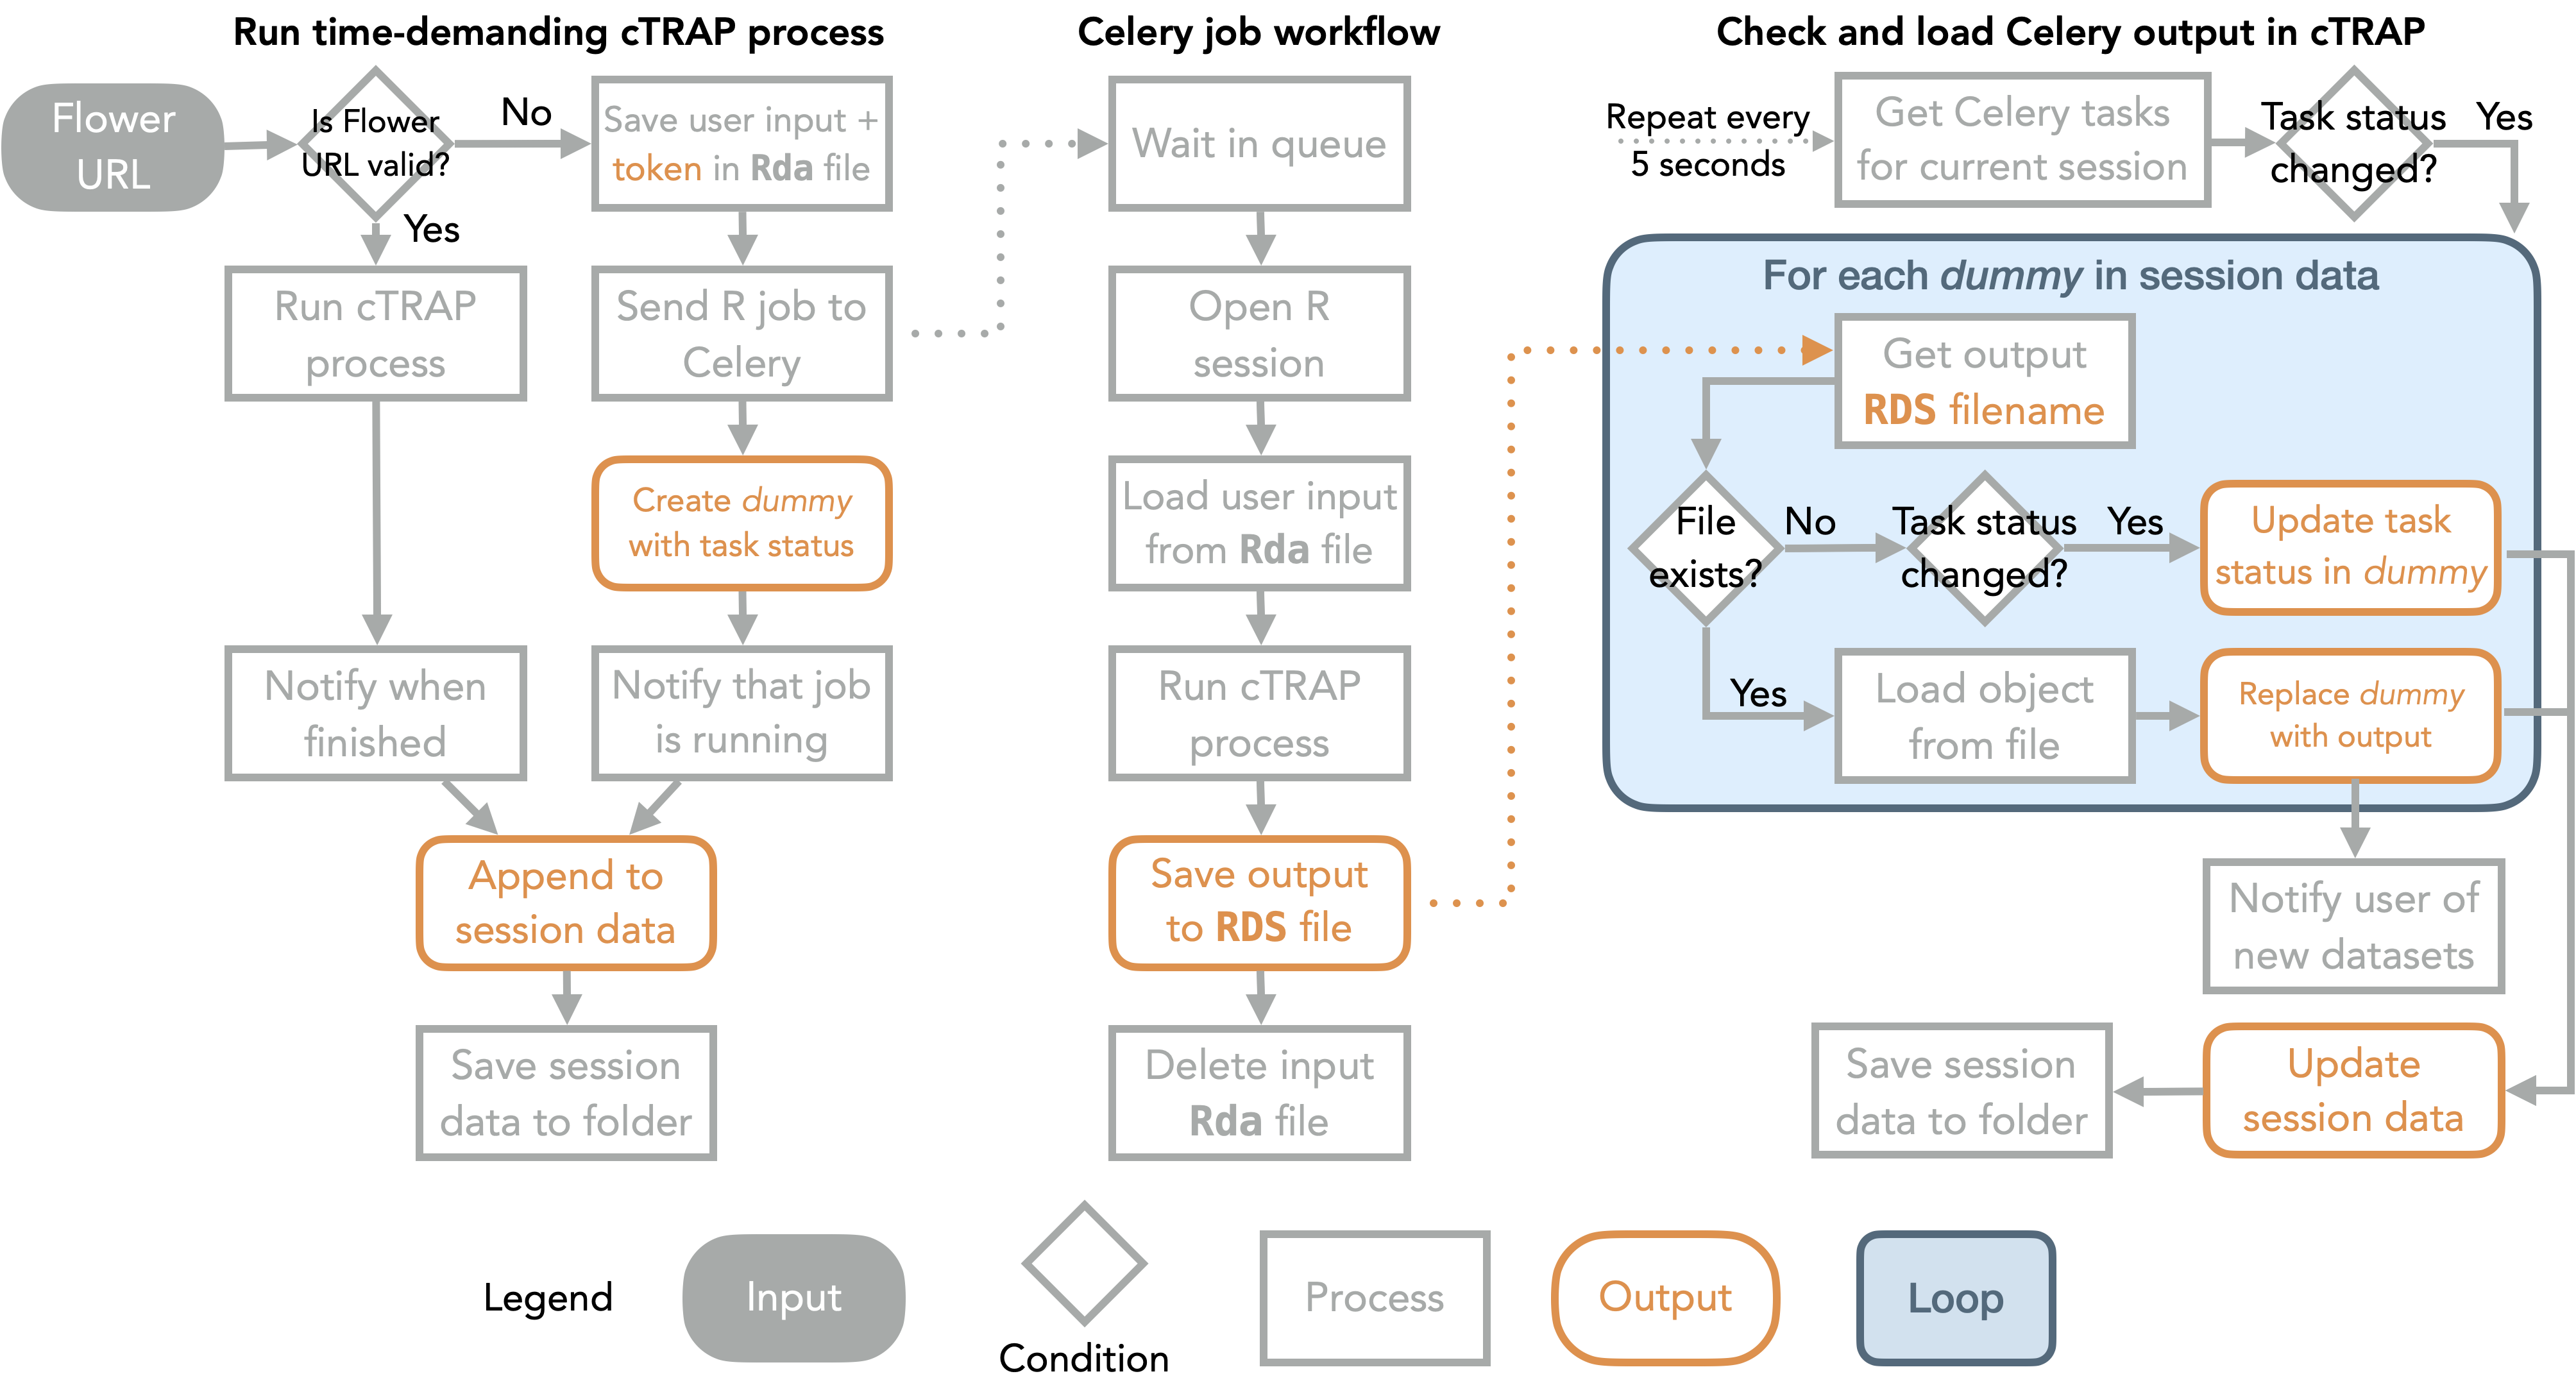
\includegraphics[width=\textwidth]{images/ctrap/celery-job}
  \centering
  \caption[cTRAP process running in Celery]{\textbf{cTRAP process running in Celery.} Time-demanding cTRAP processes can be run in the background using Celery/Flower. While running in Celery, the output of the cTRAP process is saved to the folder associated with the token of the user's session. When that specific session is active, all finished files are automatically loaded as part of the data session and the user is notified.}
  \label{fig:ctrap-celery}
\end{figure}

\section{Conclusion}

% what is your main finding (ANSWER)
% how are your findings with respect to the literature (POSITIONING)
% - RESULT: the actual results
% - CONTEXT: literature search
% - LINK: between my findings and what is known
% - INTERPRETATION: where you pinpoint, suggest, propose...
% what is your main contribution (CONTRIBUTION)
% what are the limitations (LIMITATIONS)
% what are the next steps (ENDING/FUTURE WORK)

CMap is a repository of gene expression signatures for thousands of genetic and pharmacological perturbations. Although \alink{clue.io} already exists a collection of web apps to explore CMap data and to compare user-provided results against CMap database, their tools lack X, Y and Z.

To overcome such issues, we present cTRAP, an open-source R package to identify causal perturbations from differential expression data. Moreover, cTRAP also allows to do other two things.

More recently, cTRAP was updated to perform these actions using a graphical user interface (also available as a web app at \alink{compbio.imm.medicina.ulisboa.pt/cTRAP}), besides its traditional command-line interface. From our previous experience with psichomics, we presume that the graphical interface will be popular among users that are not comfortable with coding in R or simply want to quickly check stuff.

cTRAP's drug set enrichment analysis is currently limited to molecular descriptors for the compounds from CMap and NCI-60.

For future cTRAP iterations, it would interesting to support CMap LINCS 2020, an expansion of the current CMap dataset that is described as a \emph{3-fold expansion on the previous resource, and notable new subsets of data include CRISPSR knockout of \textgreater 5k genes and hematopoietic and non-cancer cell models} (\alink{clue.io/data/CMap2020\#LINCS2020}). However, this dataset is still considered beta and would require to update the infrastructure of cTRAP given they now provide different perturbations types in separate files.

Moreover, the web app could be more useful if able to send automatic emails to users when a job finishes or raises an error, requiring to set up an email address to which to send emails from.

With the work described here, we hope that users can unravel the potential of cTRAP to identify candidate causal perturbations and compounds to better understand biological mechanisms, as well as prioritise therapeutic agents.

% !TEX root = ../PhD Thesis.tex
\chapter{CompBio app server}
\label{chap:app-server}

Since I started building psichomics, I wanted my work to be publicly available as an online web app, providing users the most up-to-date version at their fingerprints, without having to install, update and manage different versions of R, Bioconductor, psichomics and all their dependencies.
%It can take an hour to install psichomics from scratch and the command line may scare the end-users for whom psichomics was created. 
Five years after the first Bioconductor release of psichomics in 2016, that vision finally came true.

\begin{figure}[!b]
  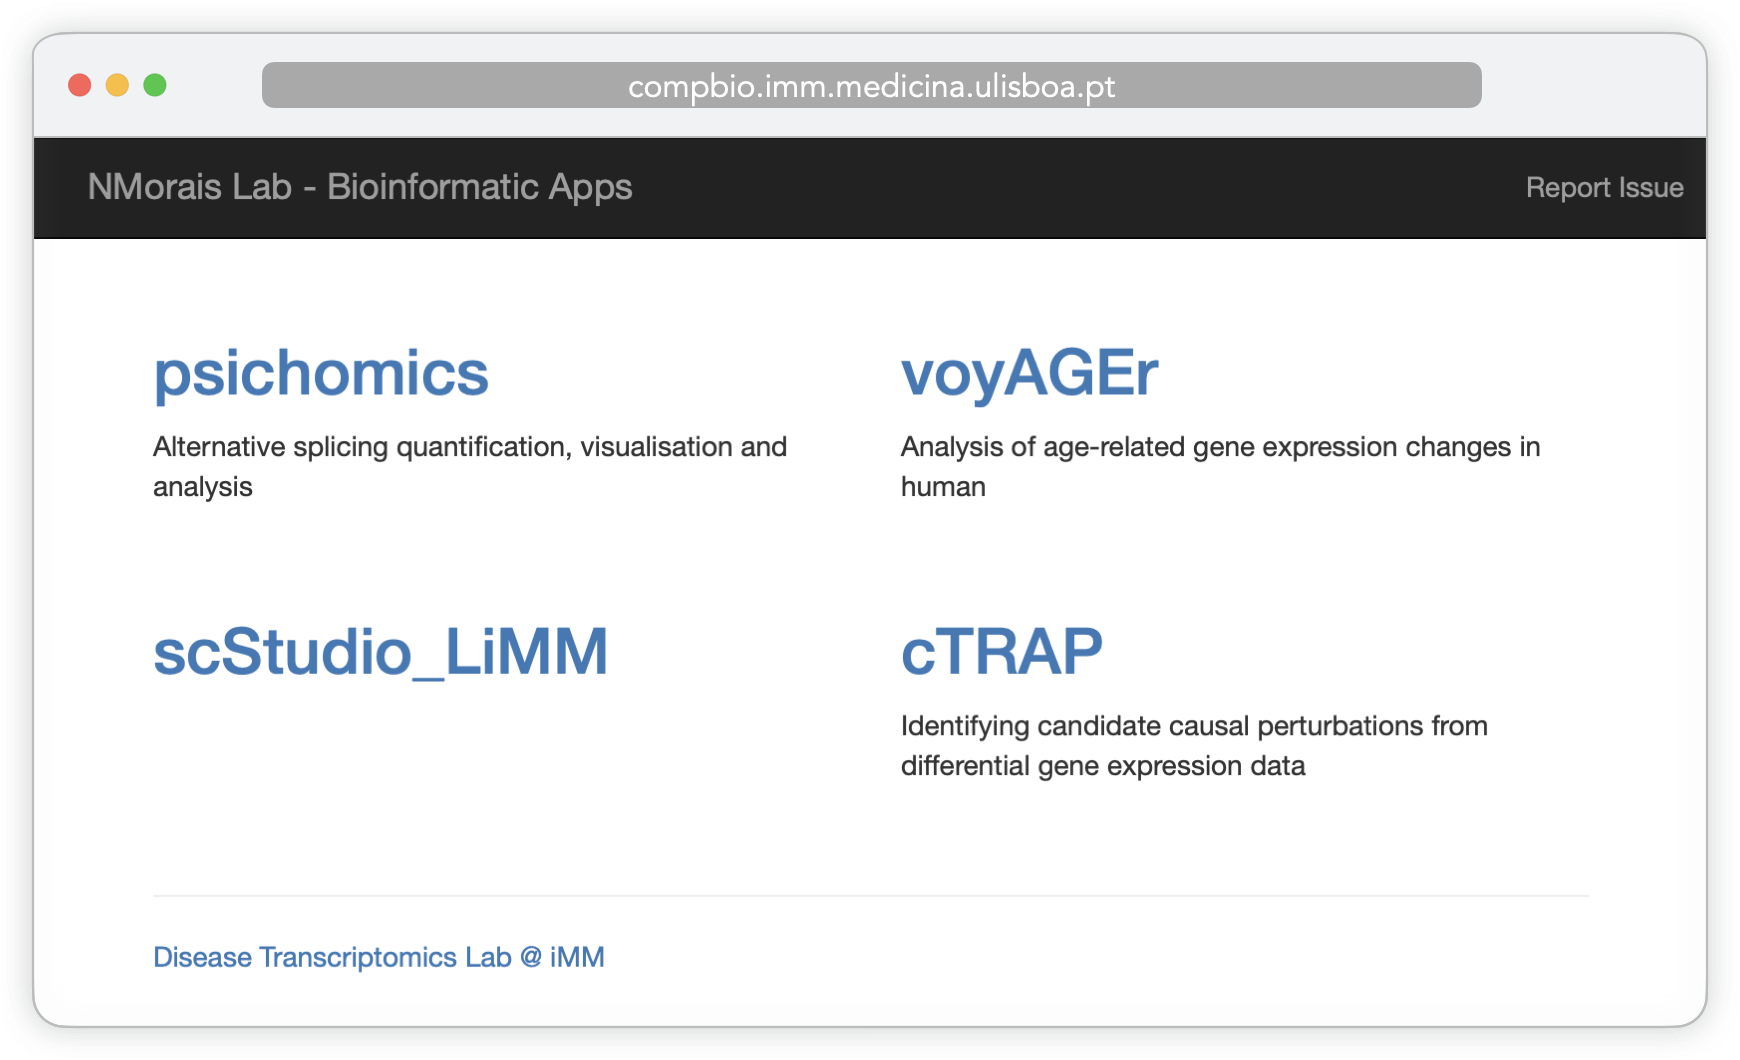
\includegraphics[width=.89\textwidth]{images/app-server/homepage}
  \centering
  \caption[Screenshot of CompBio's homepage]{\textbf{CompBio's homepage screenshot.} List of hosted web apps (11 Nov 2021).}
  \label{fig:homepage}
\end{figure}

One of our lab's ambitious goals is to develop interactive visual tools to assist in exploring biological data, either provided by users or available from big datasets. We want our tools to be used by anyone, no matter their computational background. To turn that dream into reality, I set up the CompBio app server, a Linux virtual machine running in the iMM computing cluster that hosts psichomics, cTRAP and other Shiny apps from my lab colleagues. The server is accessible at \alink{compbio.imm.medicina.ulisboa.pt} (\autoref{fig:homepage}) and its code at \alink{github.com/nuno-agostinho/compbio-app-server}.

% TODO: write specs of the app server? 200GB SSD, 64GB RAM, 16 CPU threads

\section{Background}

Our lab uses the R statistical language to analyse clinical and molecular data from public sources and collaborators. In order to share data insights with our collaborators or even the whole scientific community, we have been increasingly creating exploratory dashboards using the Shiny R package \cite{chang:2021ul}. While developing interactive Shiny web apps, it is natural to wonder: what is the best way to share them?

\subsection{Desktop apps}

Shiny apps are written in R, an interpreted programming language whose source code can run in multiple platforms \cite{r-core-team:2021wf,chang:2021ul}. When run locally, the Shiny app starts running in the device itself (\texttt{localhost}) and is accessible via a web browser. Shiny apps can be part of an R package and be provided in CRAN or Bioconductor (such as in the case of psichomics and cTRAP). Nonetheless, this requires the user to install multiple programs in their computer: R, Shiny, the Shiny app, and all their dependencies. This can take up some time if the user does not have R and many of the required libraries installed. For instance, installing psichomics in a new system can take up to 1 hour. Moreover, it still requires opening an R session to start the visual interface, which may discourage technically-challenged users to try out psichomics.

% Java (\alink{java.com}) is a platform-independent, general-purpose programming language intended to allow the same code to target multiple platforms. It uses an intermediary Java virtual machine (JVM) that translates Jave bytecode to the native platform's language. On the other hand, graphical interfaces in Java can consume more time and memory than native apps, besides having a user interface that is in stark contrast to the graphical interface of other apps.

One way to reduce the number of dependencies installed is by using Docker (\alink{docker.com}), allowing to run isolated Linux virtual environments (containers) that already contain programs and all their dependencies set up. This approach simply requires end-users to install Docker and to download the desired Docker images online. Still, Docker is a program that needs administrator privileges for installation that (1) not all users may have and (2) may not feel comfortable to give to a software they would not otherwise install.

An alternative is Electron (\alink{electronjs.org}), a software framework that allows to develop cross-platform graphical user interface apps using web technologies by combining a web browser rendering engine (Chromium, used in Chrome and other web browsers to convert HTML and CSS code into an interactive web page) and a JavaScript environment. The app itself runs the web app as if it were a usual desktop app. Some open-source projects like electricShine (\alink{github.com/chasemc/electricShine}) and photon (\alink{github.com/COVAIL/photon}) allow to convert Shiny apps to Electron apps, but they are still not fully developed and lack important features (like support for some operative systems). Regardless, compared to native apps, Electron apps are slower, have a significant overhead, take more space and consume more RAM, making Electron less attractive for intensive data-processing apps.

\subsection{Web apps}

Web apps are cross-platform, always up-to-date and can be accessed by any (modern) web browser, making access to such apps easier for end-users \cite{silva:2017wl}. However, a constantly online web server needs to be running and share its computing resources (e.g. amount of RAM, storage and CPU threads) across multiple users. The resources allocated to a web server depend on the resources consumed per app, the number of simultaneous users and the data stored per user. The price of components and their maintenance is specially relevant if anticipating a large number of end-users.

Multiple web app hosting services support Shiny apps or Docker containers of Shiny apps, including Heroku (\alink{heroku.com}) and \alink{shinyapps.io}. Both of these app hosting services offer subscription plans depending on allocated system resources, including a free plan useful to run basic apps: Heroku's free plan offers 2 threads, 512 MB of RAM and 500 MB of storage per app\footnote{According to Heroku (\alink{heroku.com/pricing} and \alink{devcenter.heroku.com/articles/limits}) as of 24 November 2021. Unverified accounts (i.e. not associated with a valid credit card) are limited to 5 apps.}, whereas \alink{shinyapps.io}'s free plan allows for 5 apps with 25 computing hours per month using 1024 MB of RAM and 1 GB of storage per app\footnote{According to official \alink{shinyapps.io} documentation (\alink{docs.rstudio.com/shinyapps.io/applications.html} and \alink{shinyapps.io\#pricing}) as of 24 November 2021.}. Such services take care of deploying the web apps and we can select a different plan to scale up the required resources to run the apps, depending on their usage. They also allow to monitor app resource usage and understand how the apps are being used and if the resources employed are sufficient or not without much effort to the developer.

Besides third-party server hosting, Shiny apps can also be deployed in local web servers. This requires server maintenance and may be harder to scale resources because of higher up-front costs. The following programs allow to locally host Shiny apps:

\begin{itemize}
	\item \textbf{Shiny Server} (\alink{rstudio.com/products/shiny/shiny-server}) is a bare-featured open-source program with only the essential features to host Shiny apps.
	\item \textbf{RStudio Connect} (\alink{rstudio.com/products/connect}) is a paid program\footnote{According to RStudio (\alink{rstudio.com/pricing}), all RStudio commercial products are free for teaching purposes and 50\% discounted for academic research from their regular bundle pricing starting at 22000\$ per year as of 24 November 2021.} with many more features than Shiny Server, including user authentication, Python-based app support and resource usage metrics.
	\item \textbf{ShinyProxy} (\alink{shinyproxy.io}) is an open-source program to host Shiny apps in Docker containers with many of the features found in RStudio Connect, including user authentication, Python-based app support and resource usage metrics.
\end{itemize}

Given that we have sufficient computing resources at our lab's disposal, we decided to build an app server -- a web server dedicated to deploy our web apps. We decided to use ShinyProxy as it has many of the advantages of using the proprietary RStudio Connect for free. Following this choice, we had to think how to properly develop the web server so it is easy to maintain, update and add new apps.

% Nginx as reverse proxy to handle all requests, including SSL certificates for HTTPS
% Nginx as a reverse proxy, serves as an intermediary between the user requests and the server.

In this chapter, I describe CompBio, our app server built with Docker Compose, a program to simultaneously manage multiple interacting Docker containers to allow for R/Shiny and Python app deployment (ShinyProxy) over a reverse proxy (Nginx), background tasks (Celery, Redis and Flower), website analytics (Plausible, PostgreSQL and ClickHouse), resource monitoring (Prometheus and Grafana), and feature testing (RStudio Web, only used to develop features and R scripts). CompBio is currently running in a virtual machine in a Linux computing cluster and hosts Shiny apps from NMorais lab, including the tools previously mentioned in this document: psichomics and cTRAP. CompBio is so named because it powers \textbf{Comp}utational \textbf{Bio}logy apps.

\section{Materials and methods}

CompBio is built using Docker Compose to manage the Docker images of multiple services: ShinyProxy, Nginx, Celery, Redis, Flower, Plausible, PostgreSQL, ClickHouse, Prometheus, Grafana and RStudio Web (\autoref{tab:compbio-services}). 
RStudio Web is only available in the development profile. The services communicate between each other via a single network created by Docker (\autoref{fig:architecture}).

\begin{table}[!h]
\small
\caption[CompBio web services]{\textbf{CompBio services.}}
\label{tab:compbio-services}
\begin{tabularx}{\textwidth}{ l l r l }
\toprule
\parnoteclear
\textbf{Role}                         & \textbf{Service} & \textbf{Port} & \textbf{Docker image}\parnote{Available in Docker Hub, unless stated otherwise.} \\
\toprule
Web app deployment                    & ShinyProxy     & 8080 & \dockerlink{openanalytics/shinyproxy}     \\ \midrule
Reverse proxy                         & Nginx          &  443 & \dockerlink[_]{nginx}     \\ \midrule
\multirow{3}{4cm}{Background tasks} & Celery + cTRAP &      & Based on \dockerlink{nunoagostinho/ctrap}\parnote{Python and Celery are installed on top of cTRAP Docker image, allowing Celery to run cTRAP analyses: see file \link{https://github.com/nuno-agostinho/compbio-app-server/blob/main/celery/Dockerfile}{celery/Dockerfile}.} \\
                                      & Redis          &      & \dockerlink[_]{redis}     \\
                                      & Flower         & 5555 & \dockerlink{mher/flower}     \\ \midrule
\multirow{3}{4cm}{Website analytics
\par(i.e. track visitor metrics)}     & Plausible      & 8000 & \dockerlink{plausible/analytics}     \\
                                      & PostgreSQL     & 5432 & \dockerlink[_]{postgres}     \\
                                      & ClickHouse     &      & \dockerlink{yandex/clickhouse-server}     \\ \midrule
\multirow{4}{4cm}{Resource monitoring} & Prometheus     & 9090 & \dockerlink{prom/prometheus}     \\
                                      & Grafana        & 3000 & \dockerlink{grafana/grafana}     \\
& Nginx monitoring & & \dockerlink{nginx/nginx-prometheus-exporter}     \\
& System monitoring  & & \dockerlink{prom/node-exporter}     \\ \midrule
RStudio (testing) & RStudio Web\parnote{Only available in the development profile.} & 8787 & Based on \dockerlink{rocker/rstudio} \\
\bottomrule
\end{tabularx}
\parnotes
\end{table}

\begin{figure}[!h]
  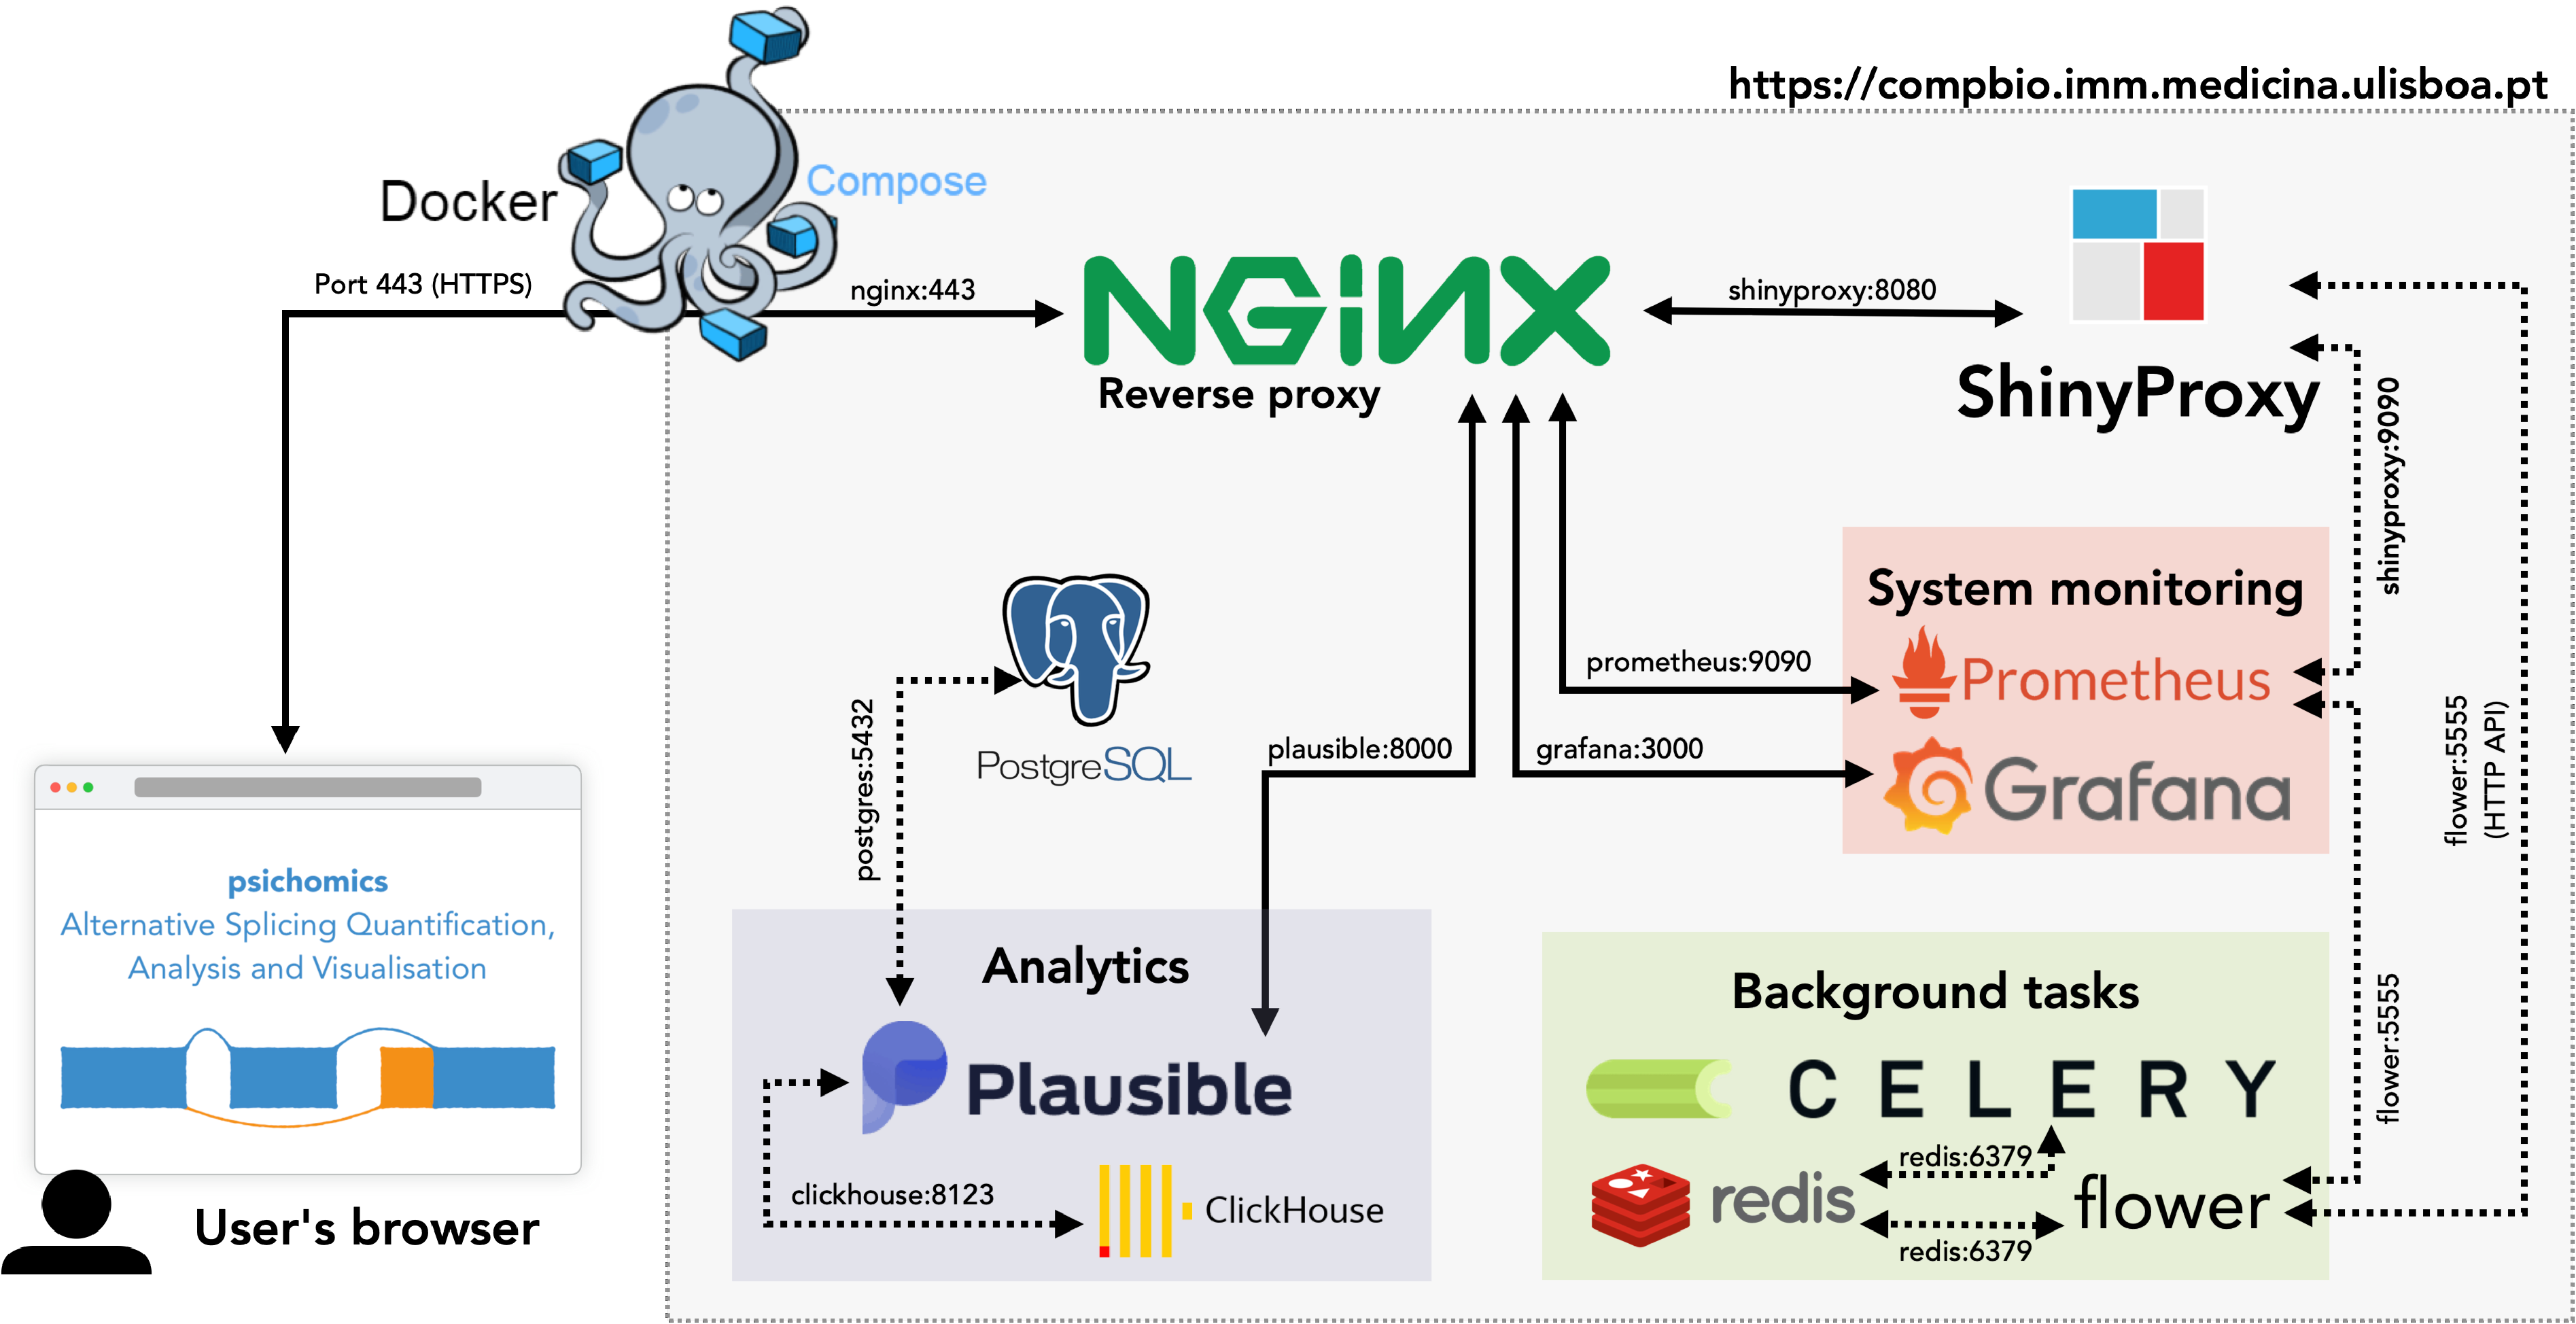
\includegraphics[width=.9\textwidth]{images/app-server/architecture}
  \centering
  \caption[App server architecture]{\textbf{App server architecture is based on Docker Compose.} All services are provided via Docker images and communicate with each other via a Docker-created network using the name of the service and a specific port (e.g. Nginx communicates with ShinyProxy via \texttt{shinyproxy:8080}). The groups  (analytics, system monitoring and background tasks) are strictly conceptual.}
  \label{fig:architecture}
\end{figure}

Services whose ports are listed in \shortref{tab:compbio-services} may be accessed when connected via an ethernet cable at iMM or via the VPN of Universidade de Lisboa by using an internal HTTP (not HTTPS) URL specifying the service port. For instance, opening \link{http://imm-nmorais-p2.fm.ul.pt:8000}{http://imm-nmorais-p2.fm.ul.pt:8000} allows to access the Plausible dashboard\footnote{If the web browser starts redirecting HTTP requests to HTTPS, the website should be accessed in private mode to avoid that behaviour, given that HTTPS disallows specifying ports.}.

\section{Results}

The CompBio app server was developed to be easily maintained and extended, allowing to add new and update existing Shiny apps and other modules. The server also supports running background processes\footnote{More information in \fullref{sec:background-tasks}.}, tracking simple visitor metrics (e.g. Shiny app usage time, number of visitors and user countries) and monitoring system usage. This project is open-source and free (\alink{github.com/nuno-agostinho/compbio-app-server}) and the app server can be publicly accessed at \alink{compbio.imm.medicina.ulisboa.pt}.

The app server makes use of a two-tiered architecture as the user interface is displayed using the user's web browser to render the HTML, CSS and JavaScript code, whereas the application and database layers are all run in the same server. The server itself is a virtual machine running in Lobo (iMM computing cluster) with 16 CPU threads, 64GB RAM and 200GB SSD. By exploiting a powerful infrastructure, the virtual machine can be manually modified to increase or decrease associated computing resources depending on system usage.

The code can be run on Linux\footnote{Although not the scope of this project, CompBio may be compatible with other operating systems.} machines with Docker Compose installed, thus making the setup easily portable and requiring minimal user setup. Docker Compose also confers modularity and maintainability to the project, given that system components are easy to update and replace without affecting other components.

\subsection{Docker Compose}

There are a lot of programs that can go into a web server. Experimenting different programs while managing their manifold dependencies to develop an healthy web server is like an intricate ballet where all finely-coordinated dancers interplay for an astounding performance: a wrong move can affect the whole show. After all, each program/dependency has its own requirements and some may be a distress to (un)install. Moreover, when the server is online, errors may arise due to configuration changes (such as new app updates), requiring a fast rollback to minimise server downtime. A solution is to use self-contained and modular programs, such as Docker containers. But how to coordinate several artists to beautifully perform the Swan Lake?

\begin{figure}[!b]
  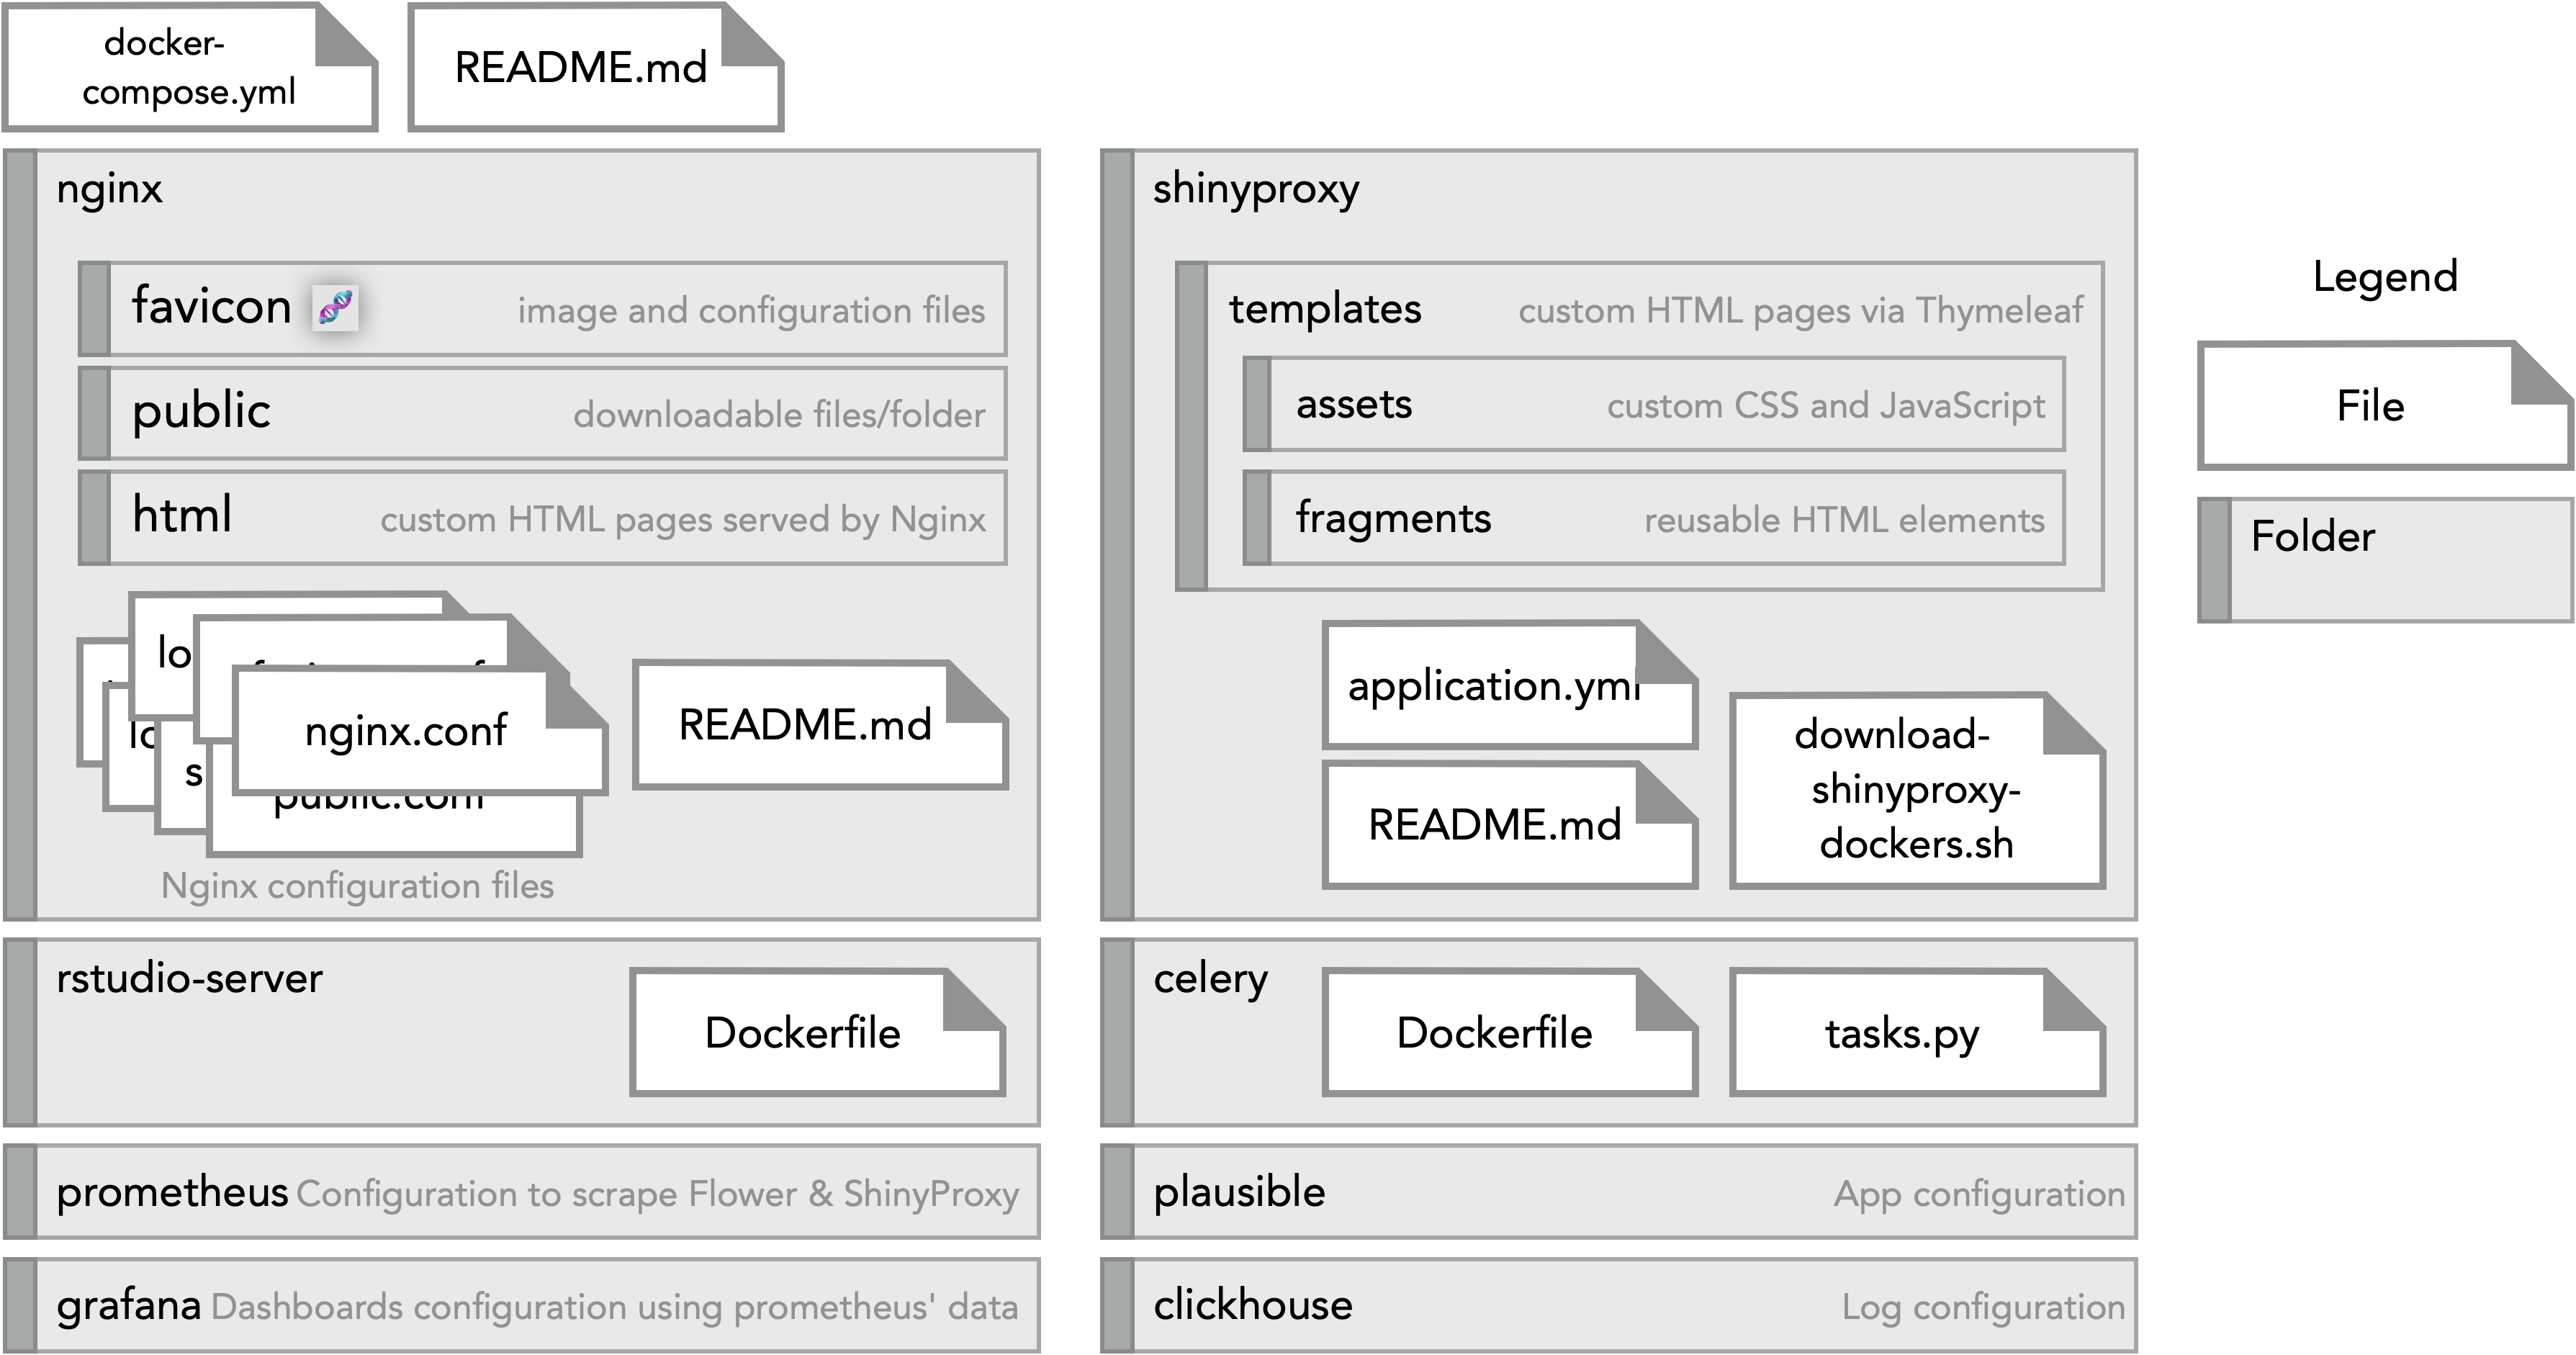
\includegraphics[width=1\textwidth]{images/app-server/file-structure}
  \centering
  \caption[App server's file structure]{\textbf{Visual representation of the file structure of the CompBio app server.} Each folder contains files associated with a specific service. Folders \texttt{rstudio-server} and \texttt{celery} contain Dockerfiles for building custom Docker images of the respective services. Multiple \texttt{README.md} document the usage of the services. The file \texttt{docker-compose.yml} in the root of the project contains the main configuration of each service.}
  \label{fig:file-structure}
\end{figure}

With the modularity from Docker Compose, multiple applications are run isolated in their own Docker containers, allowing to easily update or replace them without affecting other system components, as well as make the code of this project publicly available and portable. All services spawned in Docker Compose are based on Docker images that are either pre-created (e.g. downloaded from Docker Hub) or built on-demand -- some services of this project have their own Dockerfiles, a recipe file to create custom Docker images.

For organisation purposes, the project is structured by folders named after each service, where each folder stores files associated with the respective application (e.g. Dockerfile, configuration and data; \autoref{fig:file-structure}). A single file named \texttt{docker-compose.yml} (\shortref{lst:docker-compose.yml}) contains the main configuration of each application in the server and extra configuration files are available in the local directory.

\begin{lstlisting}[caption=Shortened version of the \texttt{docker-compose.yml} file used for the project. This version only contains the configuration for Nginx and ShinyProxy.,language=bash,label={lst:docker-compose.yml}]{docker-compose.yml}
version: "3.9"
services:
  nginx:
    image: nginx
    container_name: nginx
    restart: always
    ports:
      - 80:80
      - 443:443
    volumes:
      - ./nginx:/etc/nginx
      - /etc/ssl/imm:/certs:ro
      - ./nginx/public:/public:ro
    depends_on:
      - shinyproxy
  shinyproxy:
    image: openanalytics/shinyproxy:2.6.0
    container_name: shinyproxy
    restart: always
    ports:
      - 8080:8080
    volumes:
      - /var/run/docker.sock:/var/run/docker.sock
      - ./shinyproxy/application.yml:/opt/shinyproxy/application.yml
      - ./shinyproxy/templates:/opt/shinyproxy/templates:ro
      - shinyproxy-server:/log
      - shinyproxy-containers:/container-logs
      
  networks:
    default:
      name: shiny-net
      
  volumes:
    shinyproxy-server:
    shinyproxy-containers:
\end{lstlisting}

To start all the Docker Compose services, running the command
\begin{lstlisting}[language=bash,numbers=none]
docker compose up -d --build
\end{lstlisting}
downloads Docker images in \texttt{docker-compose.yml}, builds Docker images from Dockerfiles and starts the services in detached mode.

Although data from Docker containers is temporarily stored while the container is running, specific files and directories can be preserved in Docker volumes to avoid data loss. When starting the \texttt{docker-compose.yml} project, Docker volumes are mounted for specific directories labelled volumes in \shortref{lst:docker-compose.yml}.

Docker Compose has multiple commands to manage the associated services. For instance, to apply new configurations, it is useful to restart a single service:
\begin{lstlisting}[language=bash,numbers=none]
docker compose restart shinyproxy
\end{lstlisting}

To apply changes from \texttt{docker-compose.yml}, all services need to be restarted:
\begin{lstlisting}[language=bash,numbers=none]
docker compose restart
\end{lstlisting}

% kubernetes?
% Ansible?

\subsubsection{Secrets}

Most configuration files of the server are public, including default passwords that should only be used for testing purposes. To define sensitive information (i.e. secrets), all we need is to set custom information in a \texttt{.env} file at the root of the project directory (\autoref{lst:secrets-env}). When starting the services, Docker Compose will replace the default environment variables from \texttt{docker-compose.yml} with those from \texttt{.env}.

\begin{lstlisting}[caption=Template of a \texttt{.env} file that defines sensitive data.,language=bash,label={lst:secrets-env}]{secrets-env}
RSTUDIO_PASSWORD=rstudio_pass

POSTGRES_USER=postgres_user
POSTGRES_PASSWORD=postgres_pass

GRAFANA_USER=grafana_user
GRAFANA_PASSWORD=grafana_pass

PLAUSIBLE_EMAIL=someone@email.com
PLAUSIBLE_USER=plausible_user
PLAUSIBLE_PASSWORD=plausible_pass
\end{lstlisting}

\subsubsection{Staging and production environment}

The services in the app server (\textbf{production environment}) are live for the whole world to access. Any changes made to this server will be publicly seen by active users and should be avoided to also mitigate potential issues. Instead, changes should be tested in another system (\textbf{staging environment}), such as a personal computer in a testing environment that resembles the production one. Preparing the staging environment is easy (\autoref{lst:staging-env}) and automatically performs the following:

\begin{itemize}
	\item Creates a copy of the default Nginx and ShinyProxy configuration. This configuration files are not tracked by git and can be modified at will.
	\item Pulls and builds any Docker images used by Docker Compose and ShinyProxy.
	\item Modifies Nginx configuration to ignore SSL certificates. Nginx would throw an error otherwise because the SSL certificates only match the computer currently hosting the app server.
	\item Creates empty directories for web apps that may be populated with test data.
\end{itemize}

\begin{lstlisting}[caption=Setup testing environment.,language=bash,label={lst:staging-env}]{staging-env}
# setup files for testing and download Docker images
./setup-testing-mode.sh
# start services and RStudio in detached mode
docker compose --profile dev up -d
\end{lstlisting}

The services should be fully operational in about 30 seconds after running these commands and accessible via \alink{http://localhost} of the machine\footnote{When using a remote machine, it is necessary to set up port forwarding via \texttt{SSH} to access the remote machine's localhost.}. Some services are only available via their specific ports (\shortref{tab:compbio-services}), e.g. \alink{http://localhost:8000} for Plausible and \alink{http://localhost:8787} for RStudio.

\subsubsection{Automated Testing}

Testing is automatically performed via GitHub Actions. Every change to the GitHub repository is automatically checked to see if the command \texttt{docker compose up} works without throwing errors. In the future, automated testing could be extended to check specific functionalities of each service in the project, allowing to better understand if everything is working as expected following changes to the code.

\subsection{ShinyProxy}

ShinyProxy is an open-source program that deploys R/Shiny and Python apps via Docker. When a user starts an app, ShinyProxy creates a new Docker container exclusively for that user. The containers are automatically terminated 30 minutes (by default) after the last user interaction. ShinyProxy offers multiple built-in features, including:

\begin{itemize}
    \item \textbf{App recovery:} when restarting ShinyProxy, ShinyProxy-initiated Docker containers continue running in the background. The apps will be unavailable while ShinyProxy is not running, but will be attached to ShinyProxy once it is running again, allowing for quick server maintenance tasks\footnote{More information in \alink{shinyproxy.io/documentation/app-recovery}.}.
    \item \textbf{User authentication:} authentication with multiple methods, including social login via GitHub, LinkedIn, Google, etc. However, user authentication requires all visitors to login before continuing. As we prefer users to be able to anonymously access our apps, this feature is currently disabled.
%    \item \textbf{User sessions:} user data can be stored in user-specific folders. As the sessions are only accessible when the Docker container is already attached to the volumes, this allows for complete isolation from other user folders. This feature works best with user authentication enabled (otherwise, random identifiers are used for each visitor and requires custom logic to load data between computers).
	\item \textbf{Multiple app instances:} users can open and manage multiple app instances simultaneously (not currently enabled in the app server)\footnote{More information in \alink{shinyproxy.io/documentation/ui/\#using-multiple-instances-of-an-app}.}.
\end{itemize}

\subsubsection{Add and update web apps}

Deploying new Shiny apps in the app server is as simple as making a Docker image available in Docker Hub, pulling it to the app server and then listing it in the ShinyProxy configuration. It is important to check first if the Shiny app can be launched via the Docker image in a local machine.

Afterwards, we add the configuration of the Docker image in the ShinyProxy configuration file (\texttt{shinyproxy/application.yml}; for instance, \shortref{lst:psichomics-config}), based on the available fields from ShinyProxy. The most important fields are \texttt{id}, \texttt{display-name} and \texttt{description} to identify an app, \texttt{container-image} to identify the associated Docker image and \texttt{container-cmd} to start up the Shiny app (although the command to start up the app can be included directly in the \texttt{Dockerfile} instead). If the app requires any data, volumes can be mounted using \texttt{container-volumes}. The \texttt{container-network} should remain \texttt{"\${proxy.docker.container-network}"} for all apps, given that it is required for proper communication between ShinyProxy and Docker Compose.

\begin{lstlisting}[caption=Simplified ShinyProxy configuration with \texttt{psichomics}.,language=bash,label={lst:psichomics-config}]{psichomics-config}
proxy:
  title: NMorais Lab - Bioinformatic Apps
  template-path: /opt/shinyproxy/templates
  container-wait-time: 30000
  docker:
    internal-networking: true
    container-network: shiny-net
  specs:
  - id: psichomics
    description: Alternative splicing visualisation and analysis
    container-image: nunoagostinho/psichomics:1.18.6
    container-cmd: ["R", "-e",
      "psichomics::psichomics(host='0.0.0.0', port=3838)"]
    container-network: "${proxy.docker.container-network}"
    container-volumes: [ "/srv/apps/psichomics/data:/root/Downloads" ]
    template-properties:
      startup-time: 15s
      listed: true
\end{lstlisting}

Custom properties (\texttt{template-properties}) are also set for this project, including whether an app should be publicly listed (\texttt{listed}) and a rough estimate of its startup time to show a progress bar to visitors (\texttt{startup-time}). These custom properties are described in more detail ahead.

After defining this script, we only need to restart the ShinyProxy with \texttt{docker compose restart shinyproxy} and any configured apps will be available for use. Updating an app is as easy editing \texttt{shinyproxy/application.yml} with the most recent Docker version and pulling that version to the app server, before restarting ShinyProxy.

\subsubsection{Custom HTML pages}

Custom HTML pages are located in folder \texttt{shinyproxy/templates}. ShinyProxy uses custom files located there if available, falling back to its own default files otherwise. In other words, to get the original ShinyProxy behaviour for the default HTML pages, we only need to remove the files from that folder and restart ShinyProxy.

The HTML pages provided by ShinyProxy are based on the Thymeleaf template engine that uses HTML-like code scripting. Directly editing HTML pages provided by ShinyProxy allows to add the custom features described in the following subsections, as well as custom error pages (e.g. 404 page not found or issues when starting containers).

\subsubsection{Progress bar when loading ShinyProxy apps}

\begin{wrapfigure}{r}{.5\textwidth}
  \vspace{-\intextsep}
  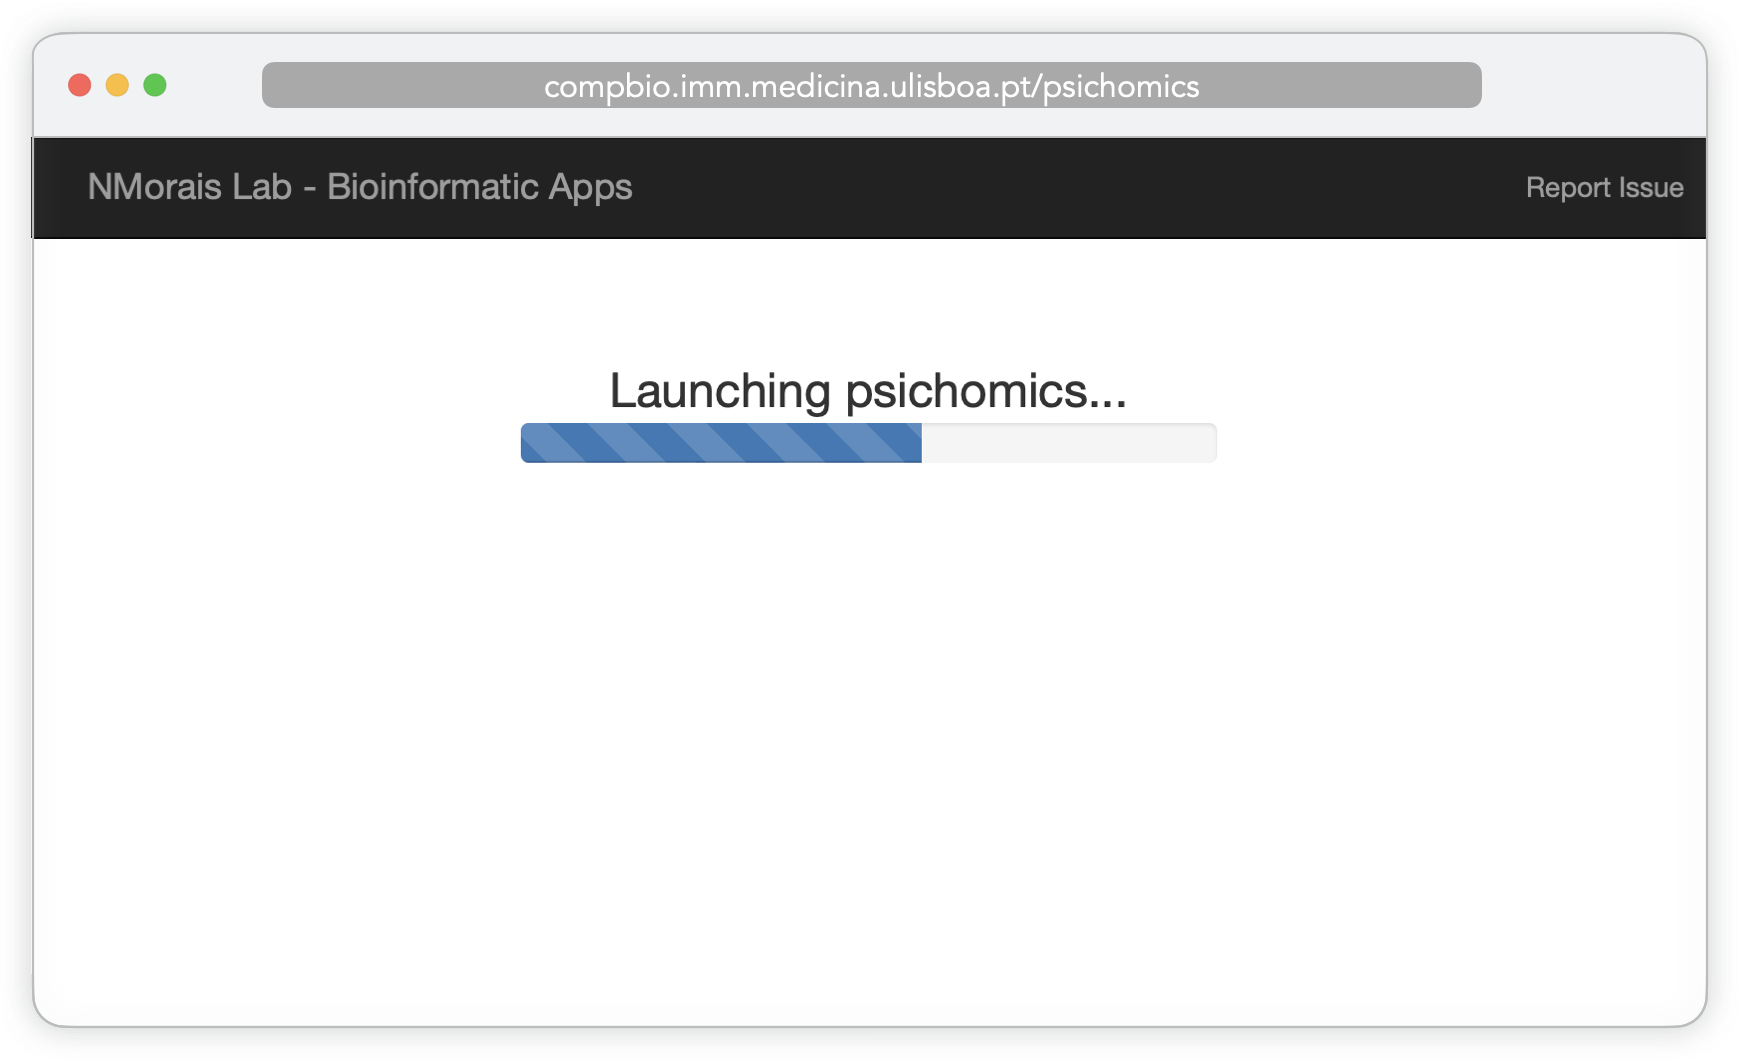
\includegraphics[width=\linewidth]{images/app-server/progress-bar}
  \caption[Screenshot of app loading]{\textbf{Progress bar displayed while psichomics loads} (11 Nov 2021).}
  \label{fig:progress-bar}
  \vspace{-\intextsep}
\end{wrapfigure}

% https://dl.acm.org/doi/pdf/10.1145/1294211.1294231
% https://www.chrisharrison.net/index.php/Research/ProgressBars2
% https://dl.acm.org/doi/pdf/10.1145/2702123.2702139
% https://www.researchgate.net/publication/234791131_The_importance_of_percent-done_progress_indicators_for_computer-human_interfaces
% https://ieeexplore.ieee.org/stamp/stamp.jsp?tp=&arnumber=6263888&tag=1

When ShinyProxy is loading an app, a spinning wheel is shown as a loading indicator. For apps that take more than 10 seconds to load (e.g. psichomics and cTRAP), the user may think the website is not working and close the window before the app is loaded. To avoid that, the spinning wheel was replaced with a progress bar to provide a time estimate for app loading (\autoref{fig:progress-bar}), making wait times more tolerable \cite{myers:1985aa,yablonski:2020ts}.

\bigskip
\bigskip

By default, the progress bar takes 5 seconds to fill (as sample Shiny apps take that much to launch in ShinyProxy), but the time is customisable for specific apps by editing the ShinyProxy configuration file (\texttt{shinyproxy/application.yml}) and adding a \texttt{template-properties.start-up} parameter to a specific app. For instance, psichomics takes 20 seconds to fully load the progress bar (i.e. \texttt{template-properties.start-up: 20s}), whereas cTRAP takes 15 seconds. When the app finishes loading, the progress bar is replaced by the app regardless of the progress displayed to the user. The accuracy of the progress bar does not need to be perfect to serve its purpose \cite{myers:1985aa,yablonski:2020ts}.

To create this progress bar, \verb|shinyproxy/templates/app.html| was edited to remove the spinning wheel and to include an empty progress bar. The progress bar's width is changed from 0\% to 100\% using JavaScript. By default, the CSS width transition applied to the progress bar is \texttt{transition: width 5s ease-in-out;} (animating a change of width that last for 5 seconds in an ease-in animation) where \texttt{5s} is replaced by the \texttt{template-properties.startup-time} parameter if set.

% \subsubsection{Report issue}

% The report issue button creates an email based on the page it is.

\subsubsection{Private web apps}

In the website's landing page (\autoref{fig:homepage}), ShinyProxy lists all apps described in the configuration file by default (\texttt{shinyproxy/application.yml}). This may not be desired when hosting apps with confidential results to be shared with specific collaborators. For this reason, we added the key \texttt{template-properties.listed} that can either be \texttt{false} (default) or \texttt{true}. The file \texttt{shinyproxy/templates/index.html} was edited to show only apps whose \texttt{template-properties.listed} key is set to \texttt{true}. Thus, non-listed web apps are not displayed in the landing page, but are still directly accessible via URL based on their app ID, e.g. \alink{compbio.imm.medicina.ulisboa.pt/app/psichomics}.

However, if the information contained in the web app should not be accessible to strangers at all, apps can also implement a password input form (e.g. \texttt{shiny::passwordInput()}) in the code itself before loading any data and/or information. That password should be securely shared with the intended audience only.

\subsection{Nginx}

Nginx is a reverse proxy, i.e. an intermediary that controls what is shown to the user depending on the URL visited -- akin to those switchboard operators seen in old movies. In CompBio, Nginx fulfills user requests and performs many other functions:

\begin{itemize}
	\item \textbf{Ensure HTTPS traffic is encrypted via SSL certificates} from the IT team at iMM. We simply point to the correct location of those certificates.%As standard practice, the certificates are composed by three parts: the site certificate, intermediate certificates, and the private key.
	\item \textbf{Serve publicly available files} in the \texttt{nginx/public} folder, whose directory structure is accessible at \alink{https://compbio.imm.medicina.ulisboa.pt/public/}.
	\item \textbf{Show a custom error page if ShinyProxy is not responding} (e.g. temporarily down or overloaded). When ShinyProxy is down, Nginx informs end-users to retry refreshing the page and that ShinyProxy is probably down, informing end-users to retry refreshing the page. ShinyProxy can be down for multiple reasons, such as during a restart or due to resource overloading. % custom HTML error page screenshot?
	\item \textbf{Display the website favicons} stored in folder \texttt{nginx/favicon}.
\end{itemize}

\subsection{Background tasks}
\label{sec:background-tasks}

In our app server, we use Celery to run background tasks, alongside Flower to manage Celery jobs via its graphical interface and HTTP API\footnote{More information in \fullref{subsec:background-tasks}.}. We also use the Redis broker to communicate between the two Docker containers.

Currently, cTRAP is the only web app in our server that exploits background tasks. We built a Docker image based on the official cTRAP Docker image (\dockerlink{nunoagostinho/ctrap}) with the Celery app installed on top.

% --max-memory-per-child
% --time-limit and --soft-time-limit
% --autoscale=10,3
Celery was configured to use 3 to 10 processes based on demand, as well as CPU and memory usage via an independent plugin (\alink{github.com/jcushman/celery-resource-autoscaler}). For instance, each process in Celery can use up to 10GiB of RAM and run up to 12 hours, thus avoiding rogue tasks.

To run other programs in Celery, we need to create a custom Dockerfile containing those programs (e.g. based on their Docker images) with Python and Celery installed. The Nginx configuration needs to include the new Celery service (\shortref{lst:celery-worker}).

\begin{lstlisting}[caption=Configuration of the Celery service for cTRAP in \texttt{docker-compose.yml}.,language=XML,label={lst:celery-worker}]{celery-worker}
  celery-ctrap:
    container_name: celery-ctrap
    build: ./celery
    command: celery -A tasks worker -c5 -l info -E -n ctrap
    volumes:
      - ./celery:/celery:ro
      - ../apps/cTRAP/sessions:/data
    depends_on:
      - redis
\end{lstlisting}

\subsection{Resource monitoring}

Prometheus monitors the server resources and the collected data can be visualised using Grafana (\shortref{fig:grafana}). The tracked resources include Celery job usage, ShinyProxy metrics (app usage time, app failures, users per app, etc.), Nginx status and Linux system resources (e.g. RAM usage, available disk space and CPU stress).

\begin{figure}[!h]
	\centering
	\begin{subfigure}[h]{0.45\textwidth} 
		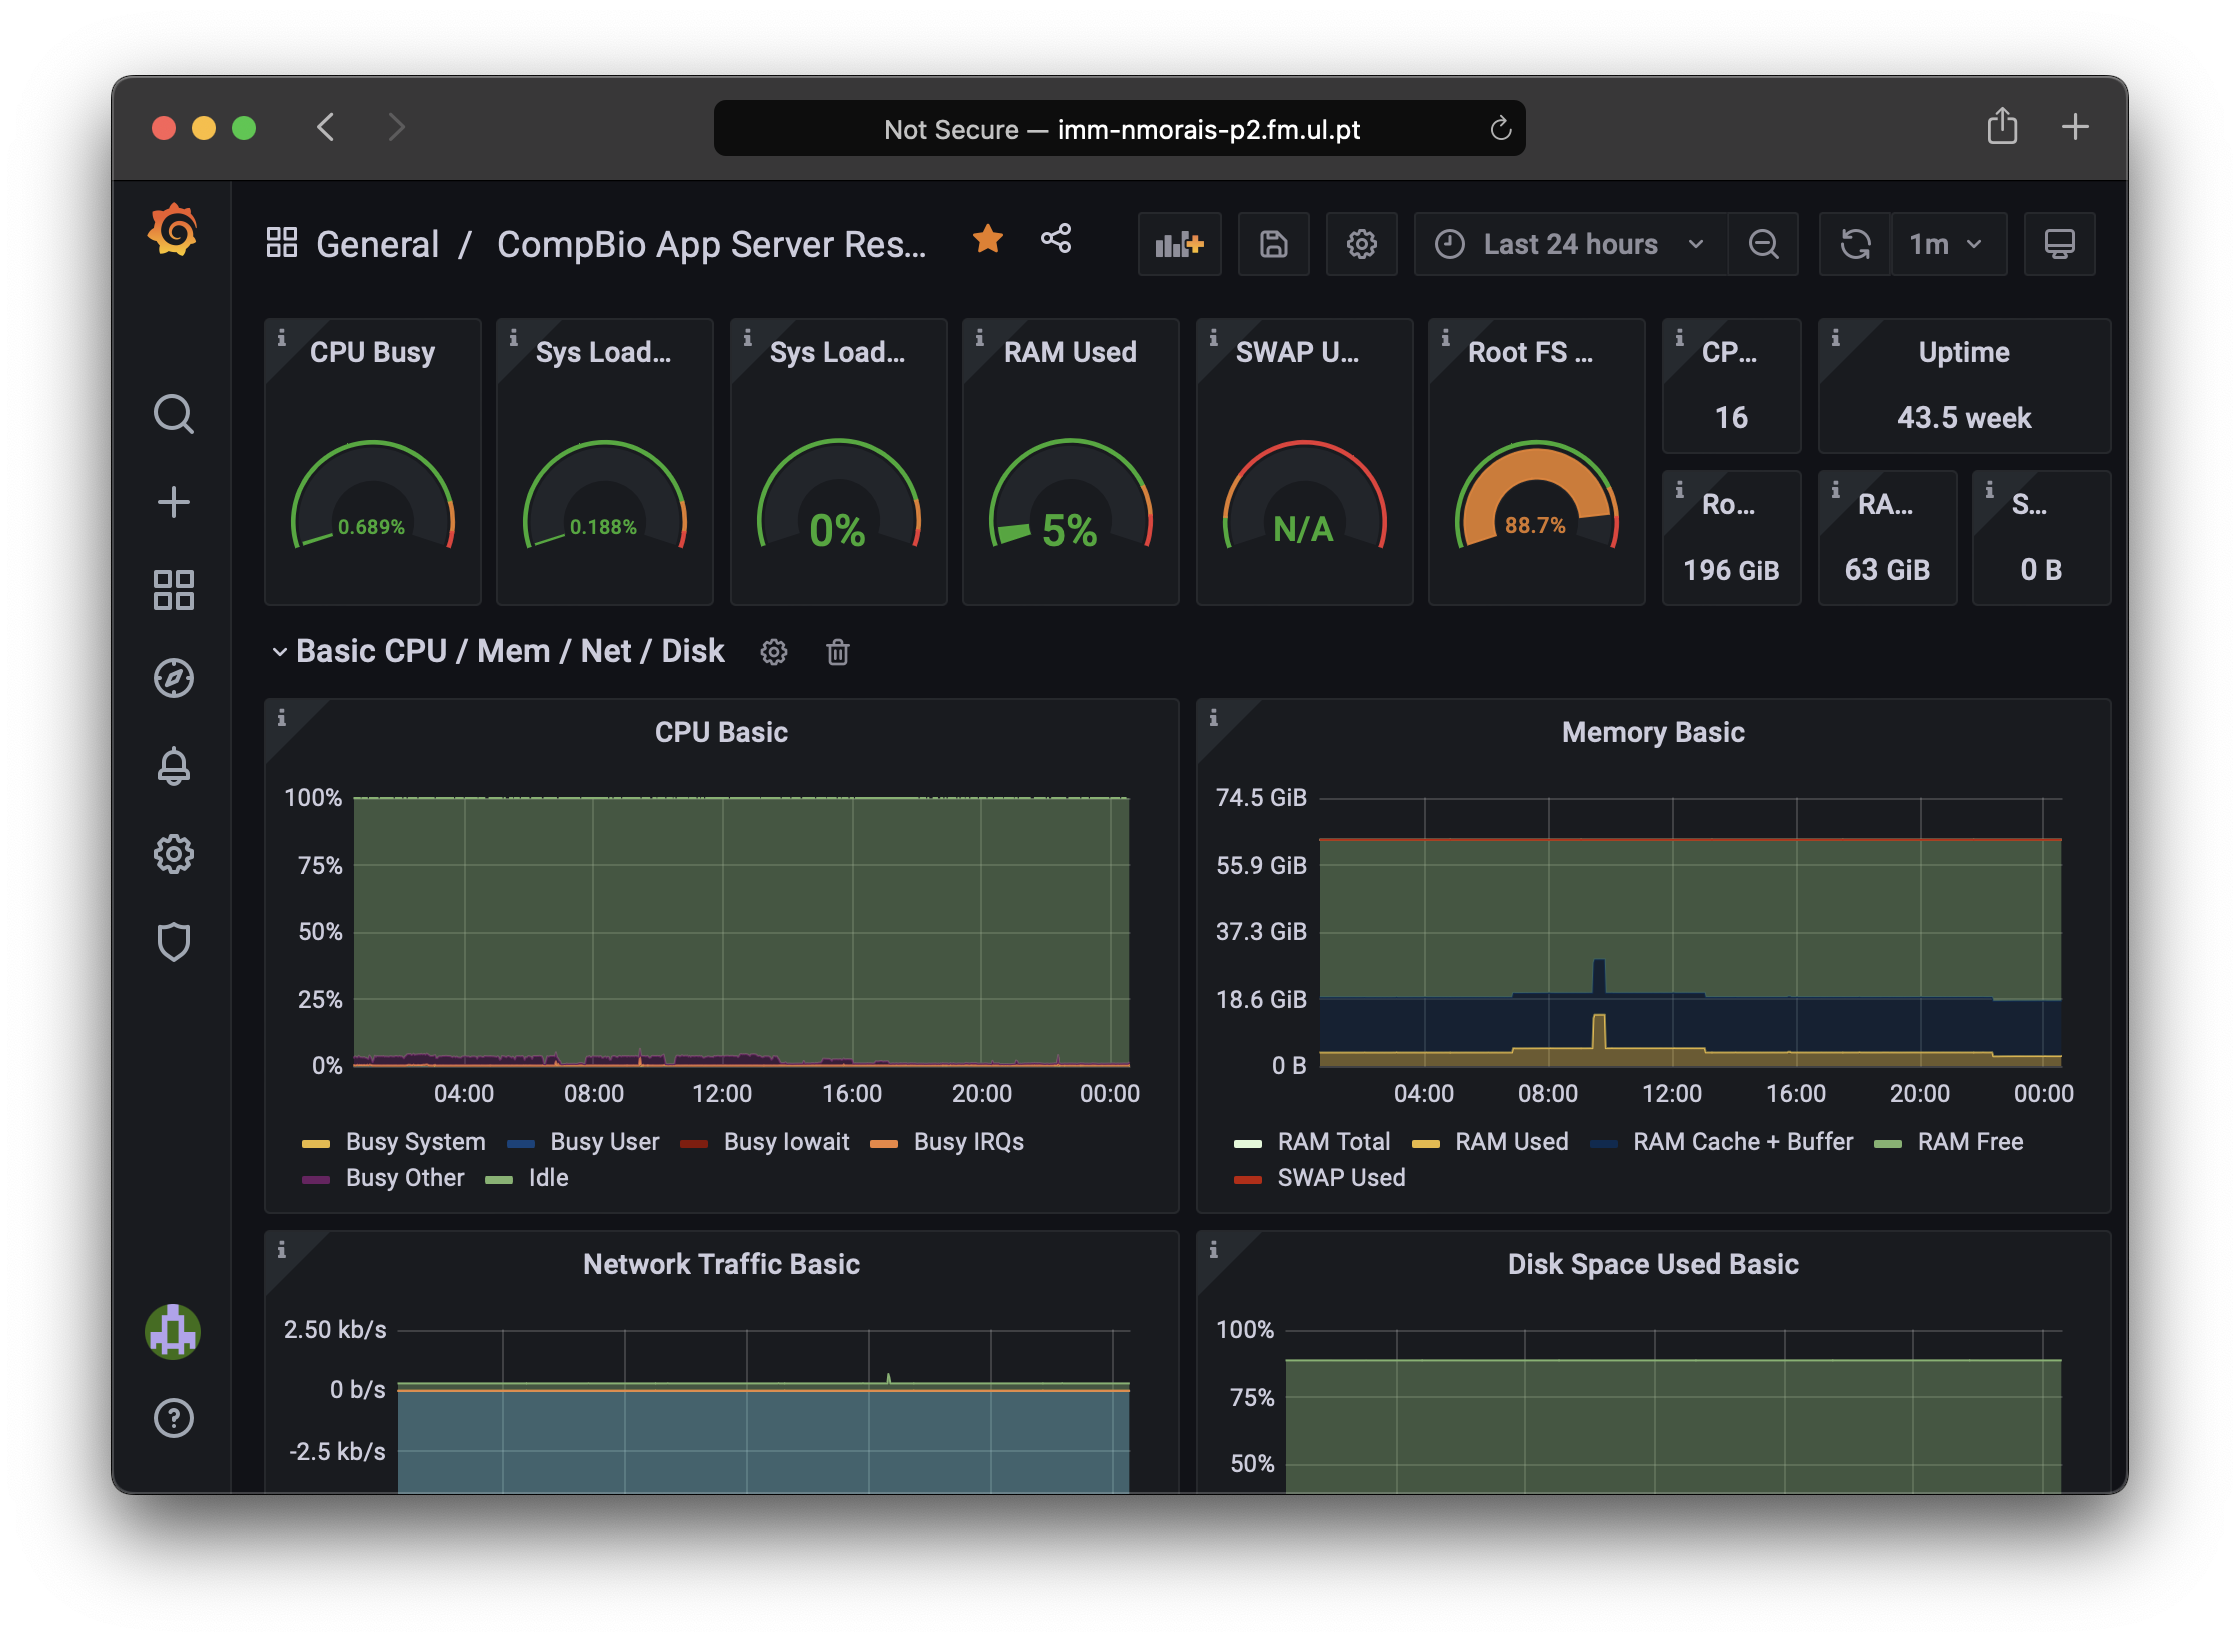
\includegraphics[width=\textwidth]{images/app-server/grafana-system}
		\caption{Linux system metrics.}
	\end{subfigure}
	\begin{subfigure}[h]{0.45\textwidth}
		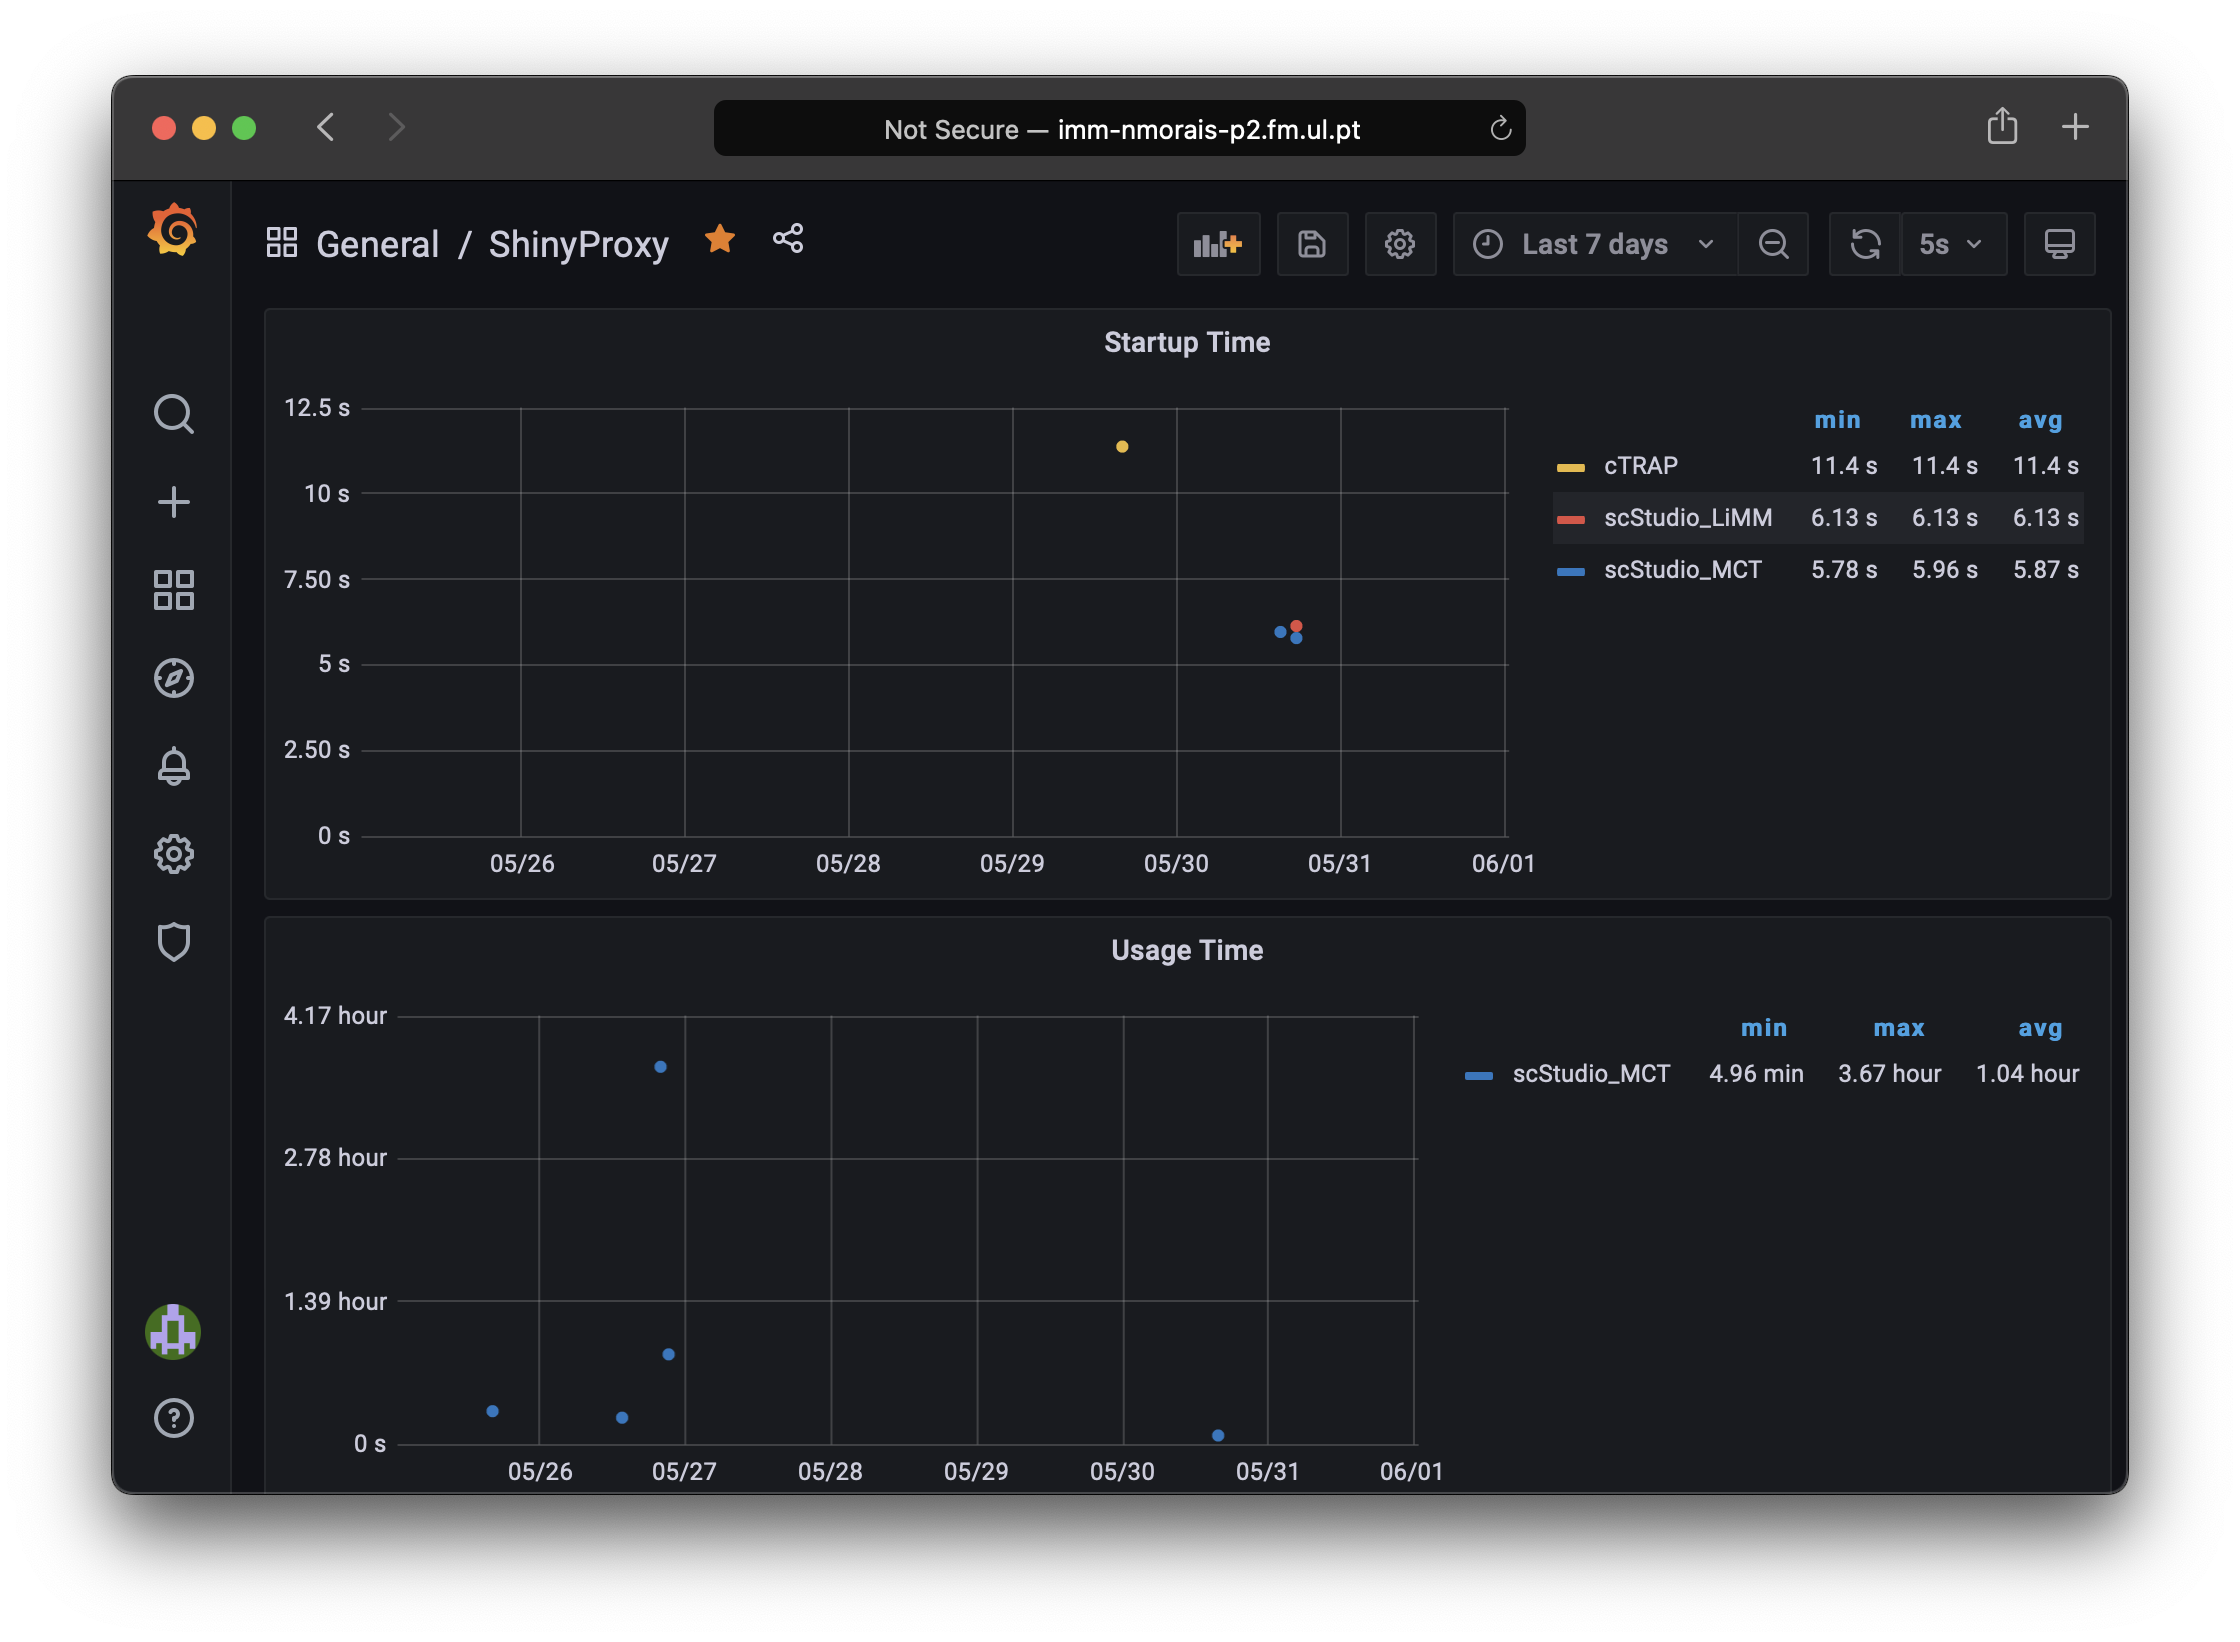
\includegraphics[width=\textwidth]{images/app-server/grafana-shinyproxy}
		\caption{ShinyProxy metrics.}
	\end{subfigure}
	\begin{subfigure}[h]{0.45\textwidth}
		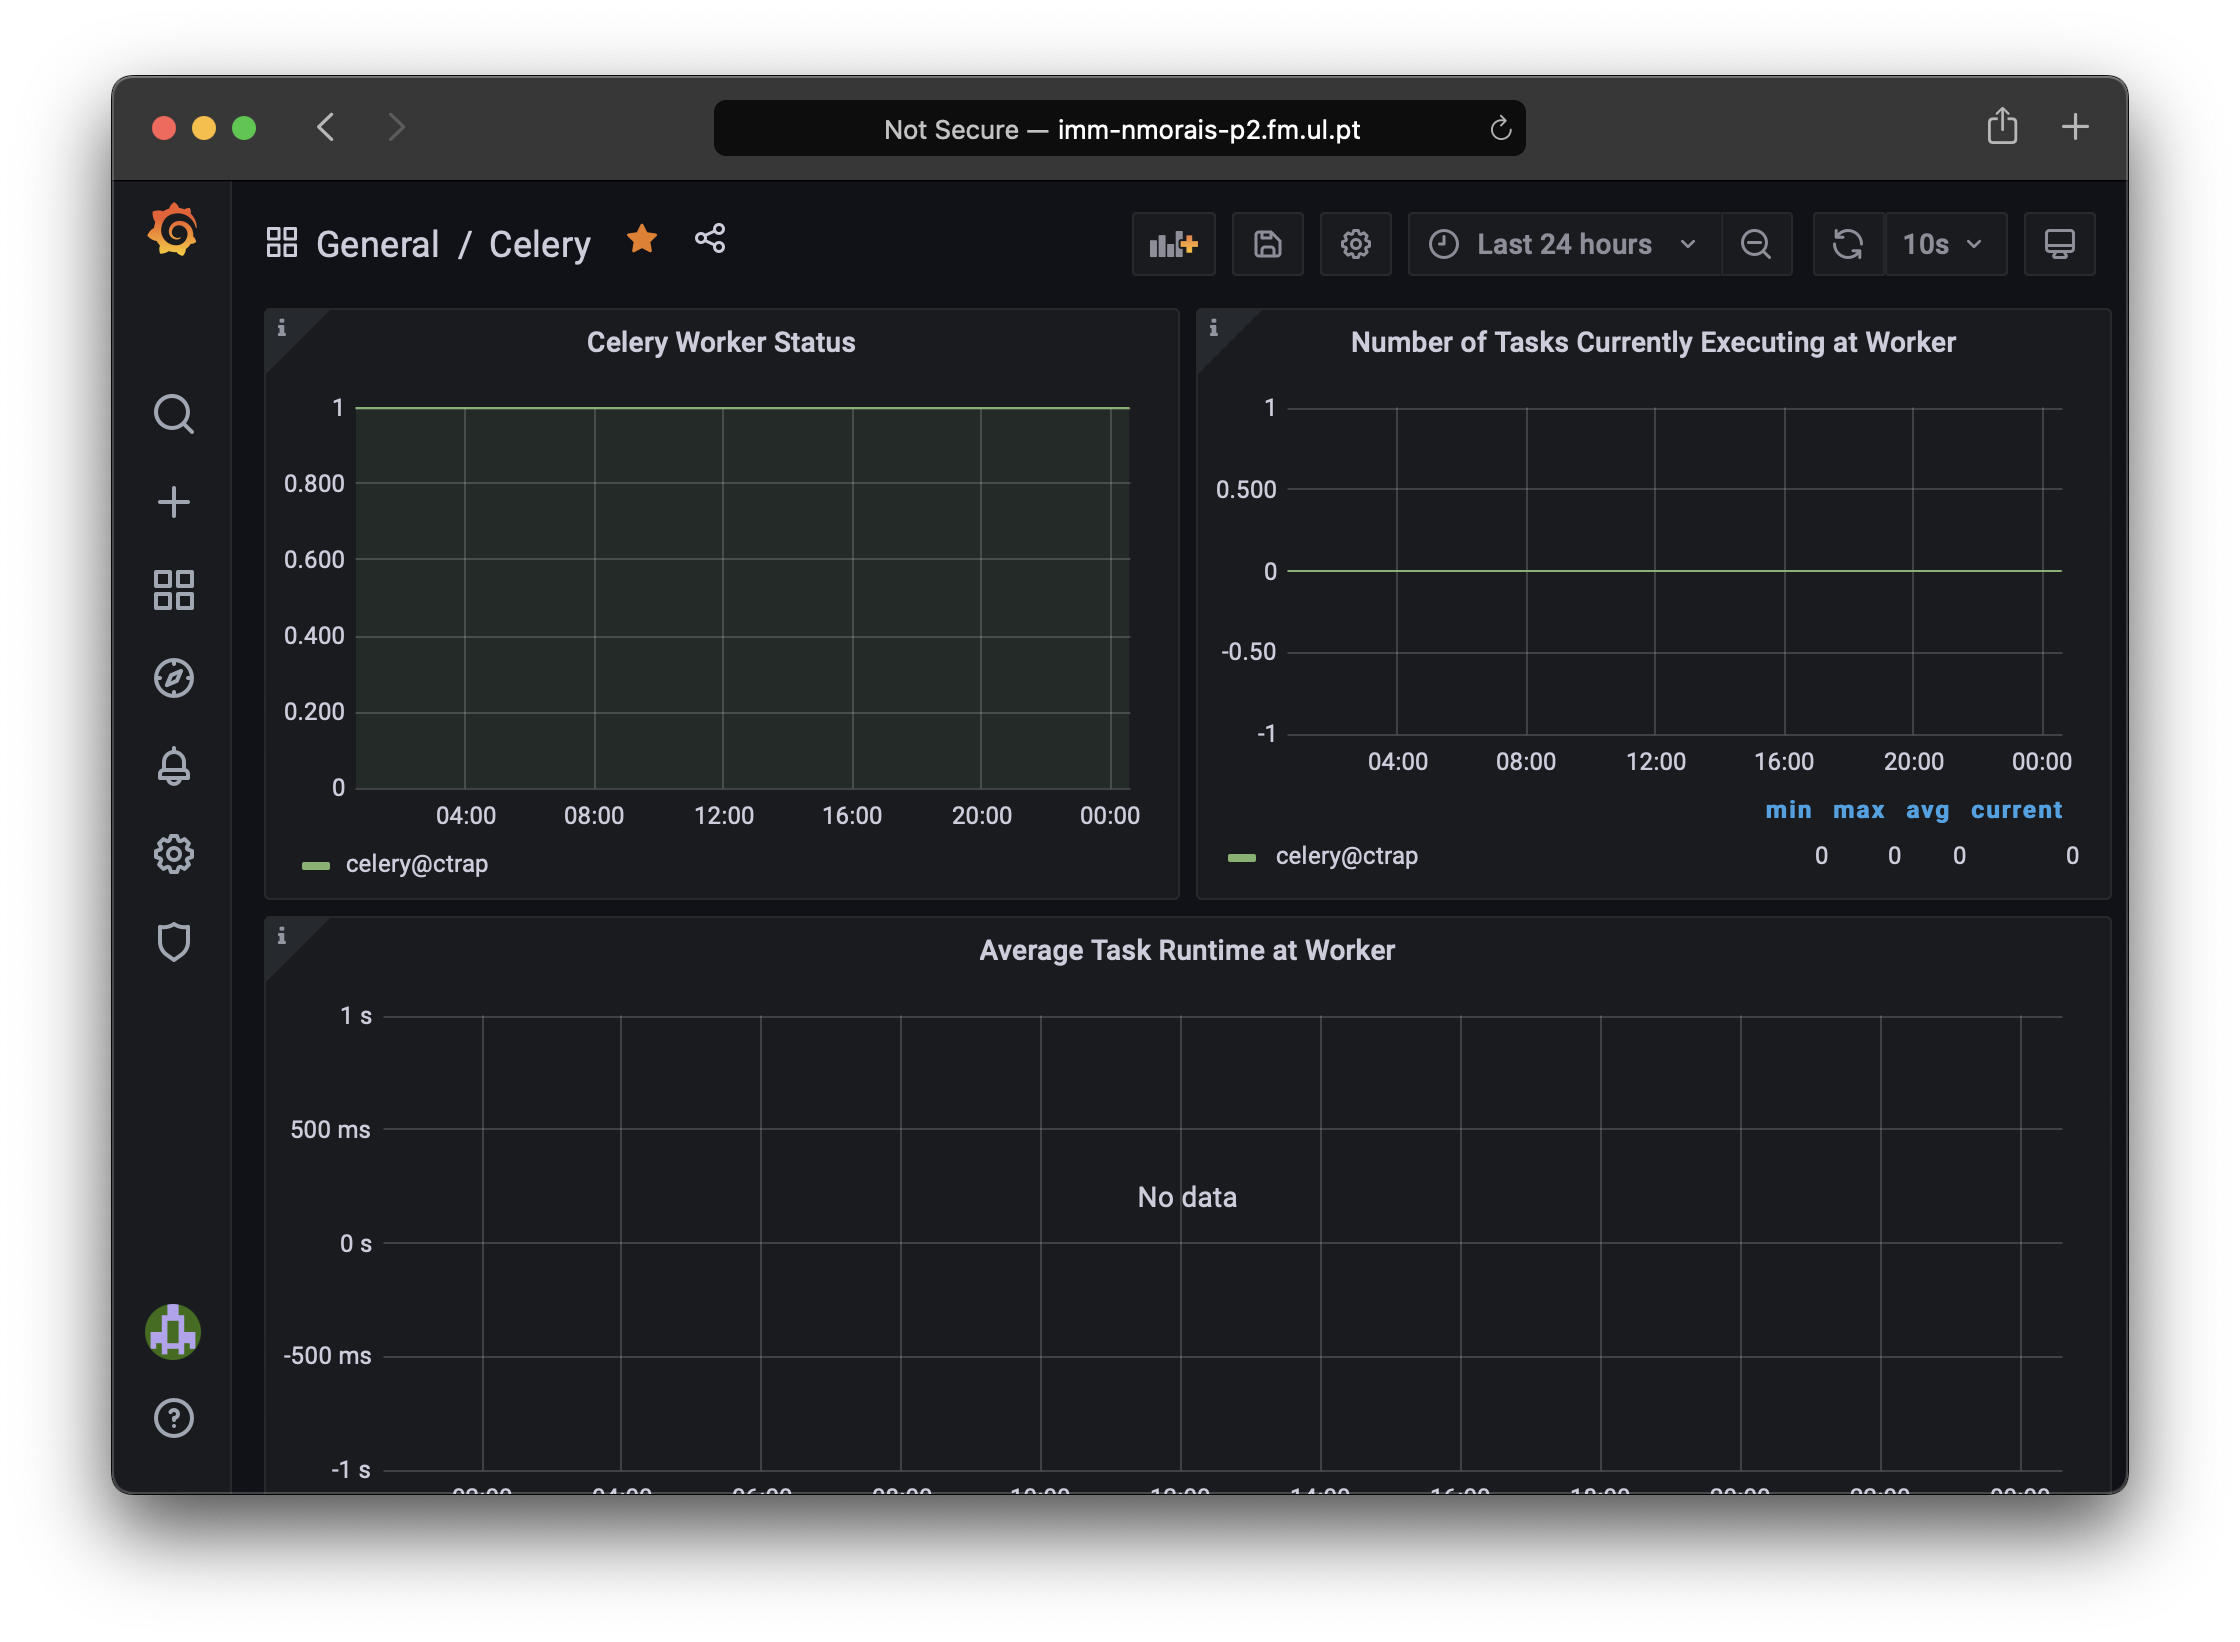
\includegraphics[width=\textwidth]{images/app-server/grafana-celery}
		\caption{Celery metrics.}
	\end{subfigure}
	\begin{subfigure}[h]{0.45\textwidth}
		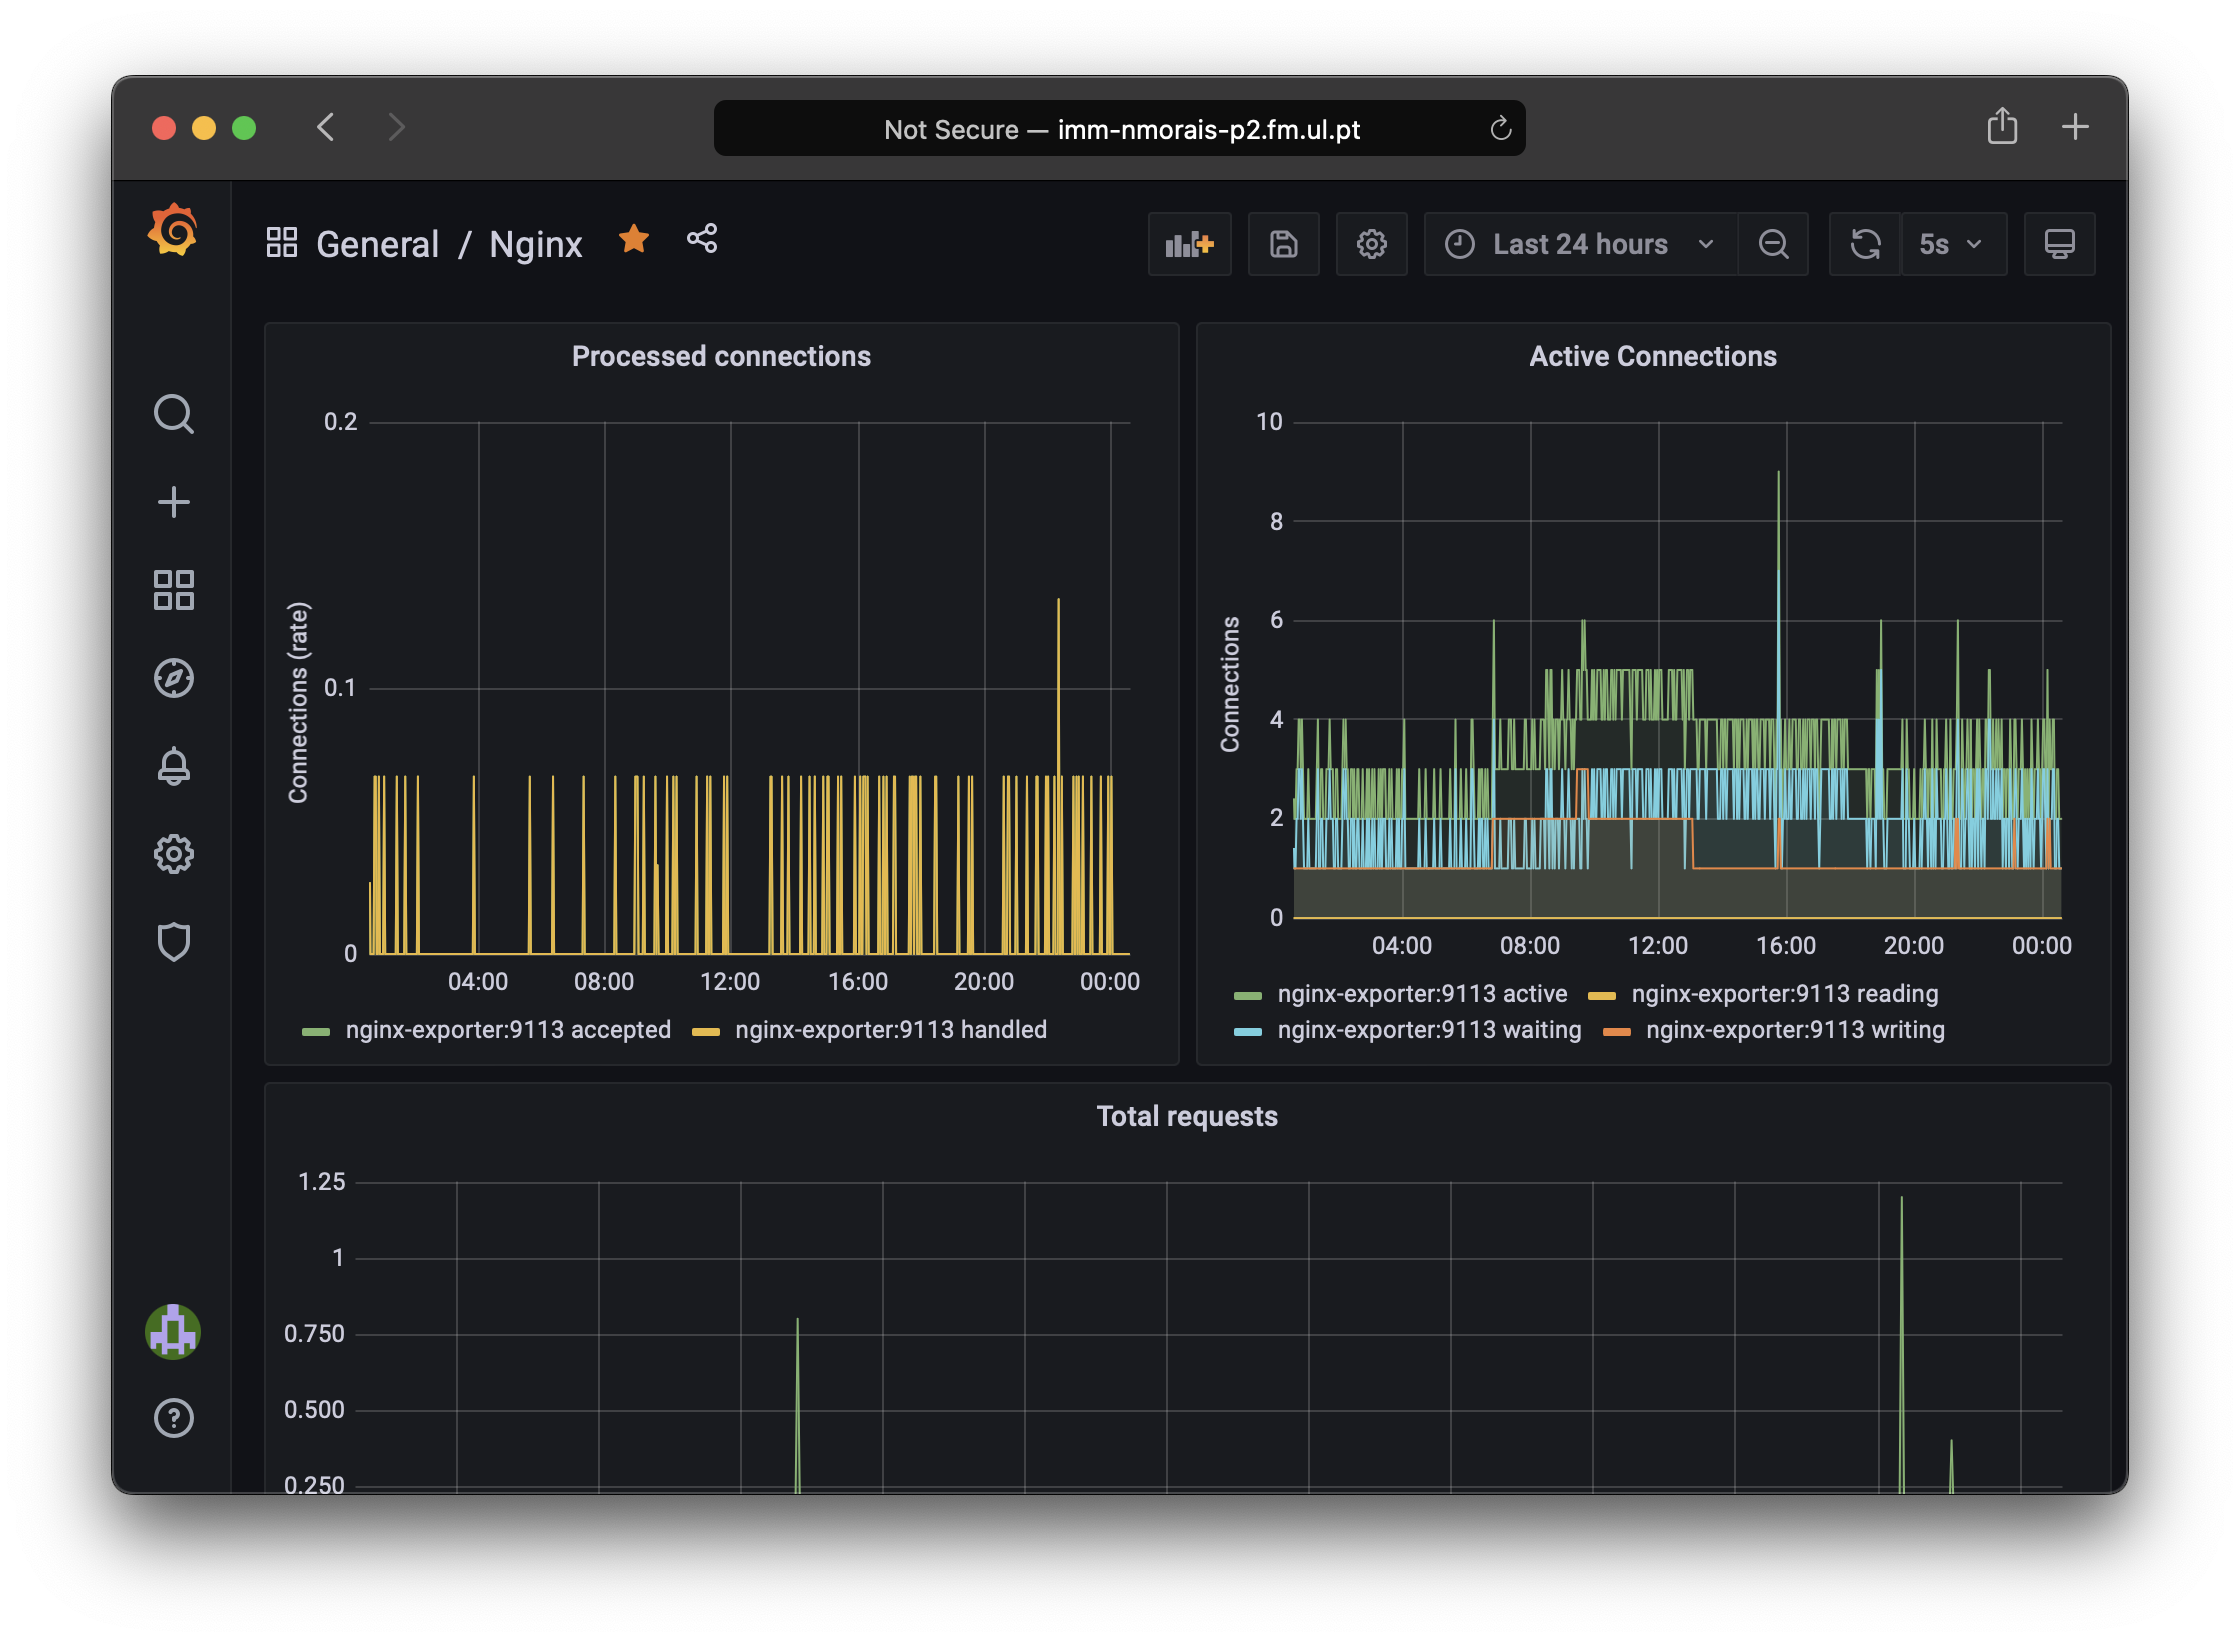
\includegraphics[width=\textwidth]{images/app-server/grafana-nginx}
		\caption{Nginx metrics.}
	\end{subfigure}
	\caption[Grafana dashboards]{\textbf{Grafana dashboards} showing tracked metrics (1 Jun 2021).}
\label{fig:grafana}
\end{figure}

\begin{wrapfigure}{r}{.4\textwidth}
  \vspace{-4\intextsep}
  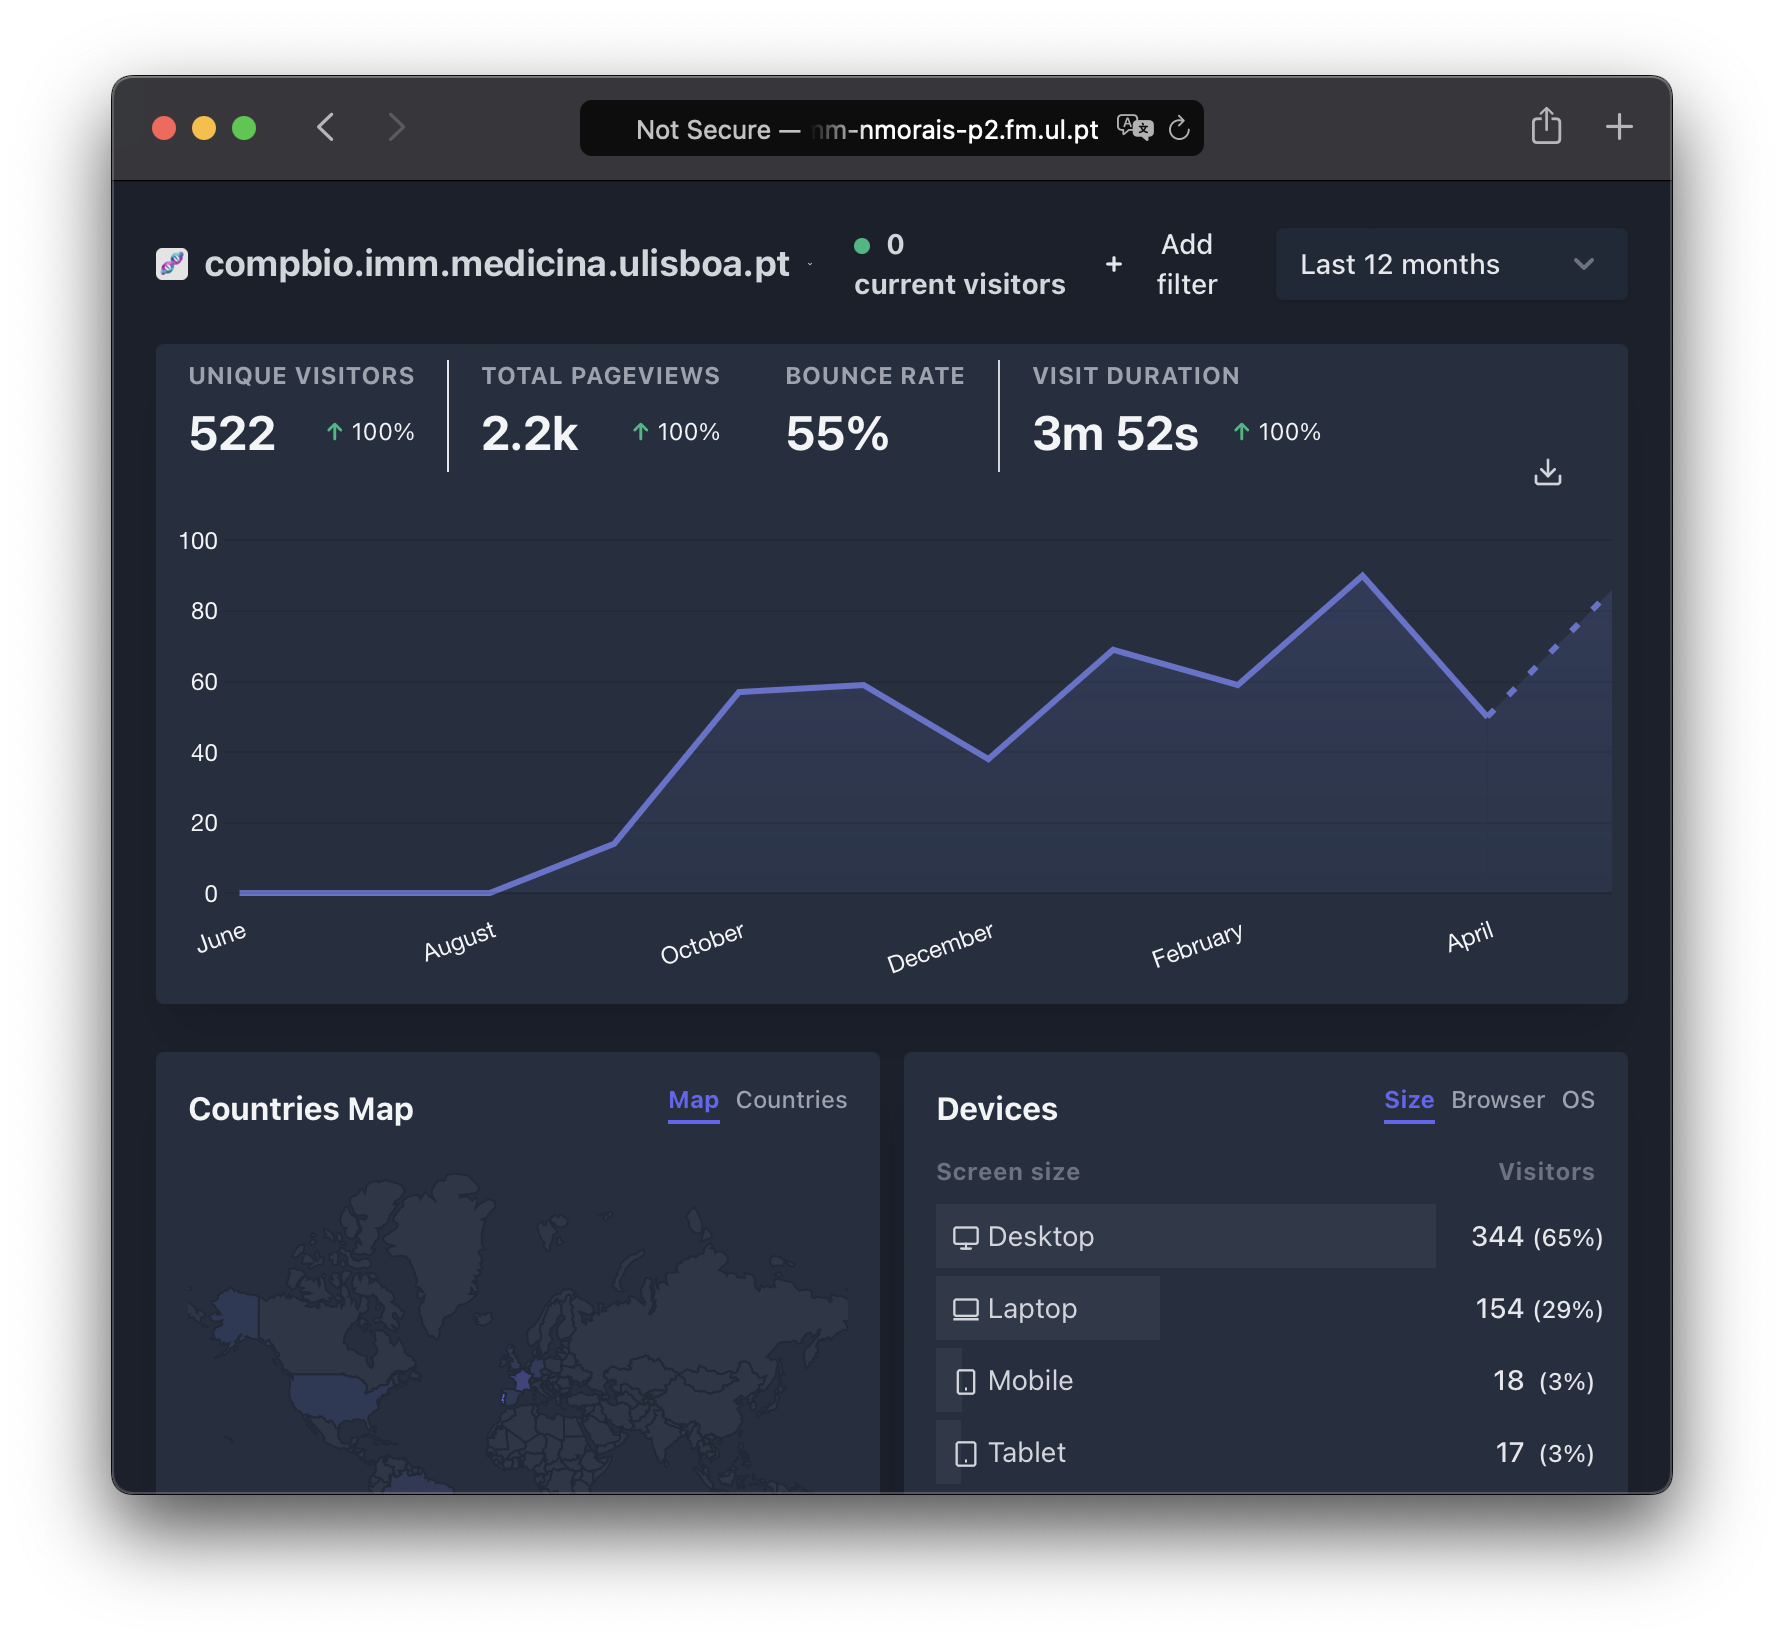
\includegraphics[width=\linewidth]{images/app-server/plausible}
  \caption[Plausible dashboard]{\textbf{Plausible dashboard} showing CompBio website analytics for the last year (as of 31 May 2021).}
  \label{fig:plausible}
  \vspace{-1\intextsep}
\end{wrapfigure}

\subsection{Website analytics}

Plausible is an open-source, privacy-focused web analytics tool that collects traffic metrics for multiple websites and provides them via an interactive dashboard (\shortref{fig:plausible}). CompBio runs the self-hosted version of Plausible. All of Plausible metrics (e.g., visitor numbers, total page views and session duration) are anonymously aggregated without cookies, thus avoiding individual tracing of users.

Plausible uses the database management systems ClickHouse and PostgreSQL to store tracking data. PostreSQL can also be used in the future as the SQL database of the server if desired, although currently no web apps in the server use this database.

Using the self-hosted version of Plausible guarantees that the tracking of user data is performed locally in the server. Plausible also protects user privacy by making their data hard to individually trace and by complying with current privacy laws. %(GDPR, CCPA and PECR).

\subsection{Server maintenance}

% TODO: Run Docker images as rootless

CompBio is a web server that hosts Shiny applications and is publicly accessible by everyone online. This makes our server a target for potential security attacks. In order to mitigate such vulnerabilities, it is crucial to update its components, including Docker, Docker Compose, Nginx and ShinyProxy. As updates may contain breaking changes that hamper website functionality, it is recommended to read change logs related to new software versions to pinpoint potential issues before updating.

% https://www.sciencedirect.com/science/article/pii/S2352484721007289#b71
% https://doi.org/10.1145/3038923
% https://www.tandfonline.com/doi/full/10.1080/19393555.2020.1853855?casa_token=EpT3lJflBXAAAAAA%3AaS5ePDNIcAPfL6MsMoKrI0s4sDtjyGNvGICZiz2Ywvnf7E2vtokORb073GUi9eilZiUCFOAqhIY

Updates to Docker and Docker Compose need to be performed by an administrator using Linux's \texttt{apt-get} command\footnote{sudo apt-get update \&\& sudo apt-get upgrade}. On the other hand, Docker images of the server (including Nginx and ShinyProxy) require a user in the \texttt{docker} group to edit the versions of the Docker images used in \texttt{docker-compose.yml} and restart the Docker Compose project\footnote{While inside the project folder: \texttt{docker compose down \&\& docker compose up -d --build}}. The advantage of using Docker Compose is that if something goes wrong with the updated Docker images, we simply need to revert \texttt{docker-compose.yml} to a previous working state and restart all services.

\section{Conclusion}

% what is your main finding (ANSWER)
% how are your findings with respect to the literature (POSITIONING)
% - RESULT: the actual results
% - CONTEXT: literature search
% - LINK: between my findings and what is known
% - INTERPRETATION: where you pinpoint, suggest, propose...
% what is your main contribution (CONTRIBUTION)
% what are the limitations (LIMITATIONS)
% what are the next steps (ENDING/FUTURE WORK)

The CompBio app server was developed to host web apps from NMorais Lab using ShinyProxy and Docker Compose, allowing to easily add new or update existing Shiny apps containerised via Docker. It also contains multiple components to run background cTRAP tasks, track app usage and monitor computing resources.

CompBio currently runs in a virtual machine in Lobo, iMM computing cluster. The hardware is taken care by the iMM IT team and they also support us with issues regarding SSL certificates, WebSocket connections and resource allocation. Moreover, I expect the server components to be easy to maintain and update. Components can be manually updated by simply editing the intended version in \texttt{docker-compose.yml} and restarting all the services. In case of issues, it is easy to rollback to a stable, working version of the app server based on previously used Docker images. Testing new changes to the server can be performed using the staging mode, allowing to mirror the app server and test changes locally before pushing them live to the app server.

The project also makes uses of Nginx as a reverse proxy. An issue with using Nginx is that it is especially verbose compared to more recent reverse proxies. Although I would have liked to replace Nginx with a simpler reverse proxy -- such as Caddy (\alink{caddyserver.com}) --, Nginx is more popular and widely used, thus making it easier to find documentation and to search for issues.

In the future, we can adapt available computing resources of our virtual machine as needed. In case we prefer to port the app server to a new machine, as the project was built on Docker Compose, relocating the app server is as easy as moving the project data to the new machine, installing Docker and Docker Compose, downloading required Docker images and starting the app server as previously indicated.

By publicly hosting the project code in GitHub, we hope to demonstrate the flexibility of setting up Docker Compose to other labs and entities, promoting an easily portable, reproducible and documented configuration of a Shiny web app server that can facilitate sharing public apps among the scientific community and beyond.


% !TEX root = ../PhD Thesis.tex
\chapter{Discussion}

Continuing the path I started walking during my MSc, my PhD gave me the opportunity to further develop web apps to be used by the scientific community and to enrich my knowledge about app development and explore multiple new technologies.

\section{psichomics}

Since starting to work in psichomics, I struggled with the lack of guidelines on how to properly design and test interactive bioinformatic web apps. Although there are resources to build generic web apps, the field of bioinformatics could be richer if we better understood how researchers and clinicians explore data to help them find what they are looking for. Also, the lack of a systematic approach to app design is notable in multiple bioinformatics programs in the wild, reflected by popular apps lacking in efficiency and usability, as well as abandoned programs due to completed and/or unrenewed grants.

Ultimately, I think that bioinformaticians that want to create apps to be adopted by the scientific community should be aware of software design to properly write apps following requirement analysis and that are designed for the long-term; data visualisation to design interactive plots that intuitively convey the desired information and allow to conveniently explore the data; and user interface design to improve the user experience and unleash the full potential of the software functionality.

psichomics was the most challenging program I ever created and the project of my lifetime. It allowed me to develop an app based on multiple topics of my interest, including transcriptomics, data visualisation, web technologies and user interface design. The positive user interaction I received, some of which have led to citations in scientific articles, and the invitation to write the methods book chapter following the publication of psichomics were uplifting and made me feel that psichomics is a good contribution to the field and I can only hope that it stays relevant and useful in the near future.

\section{cTRAP}

Thanks to working on psichomics, my knowledge of R was more mature while developing cTRAP, which allowed me to flourish my creativity. In the optimisation department, it was challenging to monitor memory usage and to improve cTRAP's runtime, reduce peak memory usage and add multicore support in order to properly perform cTRAP functions as efficiently as possible. This lead to rewriting a lot of the core code in cTRAP 1.4 (\fullref{subsec:ctrap-optim}).

Regarding its user interface, we created graphical interface functions that can be intertwined with R code, which I found a fun experiment. Although their practical usefulness may be limited, their modular design made it relatively easy to create the intuitive global interface that brought life to the cTRAP web app.

Creating the web app itself with support for background tasks via Celery and user sessions was also demanding and required a lot of experimentation to design the current implementation, including the creation of the floweRy R package to interact with Flower/Celery, testing the whole integration in the web server and to make all the code and documentation available in cTRAP so users can host their own servers with background task and user session support. Nevertheless, the web app could benefit from email support to improve the user experience, but it is not a trivial functionality as Celery does not have built-in support for sending emails.

\section{CompBio}

Creating the app server to host web apps was an enormous challenge, but I am satisfied with the final result. With the exception of R/RStudio and Docker, I had to learn about all of the software stack used (Docker Compose, ShinyProxy, Nginx, Celery\footnote{I started developing the app server at the same time I was researching how to run background tasks for cTRAP. I decided on Celery only after confirming it worked with the app server.}, Plausible, Prometheus, Grafana, etc.) and how these pieces interact amongst each other to properly fine-tune the server to our needs.

It was also interesting to configure the server to work in a testing environment so it is easy to test it on any machine before deploying to production.

\section{PanAShé}

There are many other projects that I have been part of during my PhD but unfortunately did not progress much. However, there is still one that I was a part of and I hope my colleagues will be able to complete: PanAShé.

In a collaborative lab effort, we are developing a Nextflow pipeline to process raw RNA sequencing data from TCGA \cite{chang:2013ww} and GTEx \cite{lonsdale:2013uo} in order to provide processed gene expression and alternative splicing data from samples from multiple normal and diseased tissues. The aims of this project extend those of recount2 \cite{collado-torres:2017uw} and include alternative splicing analysis, as well as a complementary dashboard to help users explore the data in these data sources. We are also considering integrating the data from this project in psichomics in lieu of the limited processed data from the public sources for TCGA and GTEx.

All the software stack in PanAShé is based on Docker images for portability and reproducibility. This means that only Docker and Nextflow are required to run the pipeline. We intend to write a peer-reviewed article regarding this project, as well as share our scripts and processed data with the scientific community as soon as possible.

\section{Conclusion}

With the work I hereby present, I hope to provide researchers and clinicians with useful tools to analyse gene expression and alternative splicing, predict therapeutic drugs and deploy web apps. Amongst my personal objectives for a PhD, psichomics has helped me complete one of them: to create something useful to someone's research. I can only hope that the rest of my work is as successful as psichomics has been in contributing to science.

As small as all my contributions may have been, these last 4 years were worthy for the prospect of having a (tiny little bit) part in helping unraveling the biological mysteries of this world, along with everything I learned and all the friends I made and danced with along the way.


% citations using BibTeX
\bibliographystyle{plos2015}
\twocolumn
{\footnotesize
\bibliography{refs}}
\onecolumn

%\appendix
%\chapter{Appendix}
%\input{chapters/appendix}

\end{document}
